\documentclass[aspectratio=169,xcolor=dvipsnames]{beamer}
\usetheme{SimplePlus}

% Math
\usepackage{nicefrac}

% Tipography stuff
\usepackage{booktabs} % Allows the use of \toprule, \midrule and \bottomrule in tables
\usepackage[english]{babel}
\usepackage{csquotes}
\usepackage{microtype}
\usepackage{pdfpages}
\usepackage{fontawesome5}
\usepackage{soul}
\usepackage{euler}
\usepackage{algorithm2e}
\usepackage{animate}
\usepackage{ifthen}
\usepackage{multirow}

% Bibliography
\usepackage[giveninits,style=authoryear-comp,backend=biber]{biblatex}
\addbibresource{../fracbiblio.bib}
\newcommand\unnumbered{\setbeamertemplate{footline}{}}%\addtocounter{framenumber}{-1}
\renewcommand*{\bibfont}{\normalfont\small}

% Figures
\usepackage{tikz,pgfplots}
\usetikzlibrary{calc,arrows,patterns,matrix,external}
\usepackage{subfig}
\usepackage{graphicx} % Allows including images
\usepackage[american]{circuitikz}
\usepackage{tikz-network}
\tikzexternalize[prefix=Figures/] % activate and define figures/ as cache folder
\usepackage{mathtools}

% Links
\usepackage{hyperref}
\hypersetup{colorlinks,linkcolor=,urlcolor=MidnightBlue}

% Code
\usepackage{minted}

% Block matrices
\newcommand{\bigzero}{\mbox{\normalfont\Large\bfseries 0}}
\newcommand{\rvline}{\hspace*{-\arraycolsep}\vline\hspace*{-\arraycolsep}}
\newcommand{\R}{\mathbb{R}}
\newcommand{\bone}{{\bf 1}}
\newcommand{\evec}{{\bf e}}
\newcommand{\dvec}{{\bf d}}
\newcommand{\xvec}{{\bf x}}
\newcommand{\yvec}{{\bf y}}
\newcommand{\qvec}{{\bf q}}
\newcommand{\svec}{{\bf s}}
\newcommand{\pvec}{{\bf p}}
\newcommand{\tvec}{{\bf t}}
\definecolor{Ao}{rgb}{0.0, 0.5, 0.0}
\setlength{\tabcolsep}{0.3em}


\author{Fabio Durastante}
\title{An introduction to fractional calculus}
\subtitle{Fundamental ideas and numerics}
\institute{Università di Pisa\\\href{mailto:fabio.durastante@unipi.it}{\faEnvelope\;fabio.durastante@unipi.it}\\\href{https://fdurastante.github.io}{\faFirefox\;fdurastante.github.io}}
\date{September, 2022}

\newcommand{\de}{{\rm d}}


\begin{document}

{\unnumbered
\begin{frame}[t,plain,noframenumbering]
\titlepage
\vspace{-4em}
\includegraphics[width=2cm]{frame.png}
\end{frame}
}

\section{Solving linear system with Toeplitz-like matrices}

\begin{frame}{Solving linear system with Toeplitz-like matrices}

In the last lecture we discretized
\begin{equation*}
	\begin{cases}\frac{\partial W}{\partial t} = \theta\,{}^{\only<1>{RL}\only<2->{\alert<2>{GL}}}D_{[0,x]}^\alpha W(x,t) + (1-\theta) {}^{\only<1>{RL}\only<2->{\alert<2>{GL}}}D_{[x,1]}^\alpha W(x,t), \qquad \theta \in [0,1],\\
		W(0,t) = W(1,t) = 0, \qquad W(x,t) = W_0(x).	
	\end{cases}
\end{equation*}
\onslide<2>{Obtaining
\[
\left( I_N - \frac{\Delta t}{h_N^\alpha} \left[ \theta G_N + (1-\theta) G_N^T \right] \right) \mathbf{w}^{n+1} = \mathbf{w}^n
\]
with
\[
G_N = \begin{bmatrix}
	1 & 0 & \cdots & \cdots & 0 \\
	g_2 & g_1 & g_0 \\
	\vdots & \ddots & \ddots & \ddots\\
	\vdots &  & \ddots &  \ddots & g_0 \\
	g_{N-1} & \cdots & g_3 & g_2 & g_1 \\
	0 & \cdots & \cdots & 0 & 1
\end{bmatrix}.
\]}
\end{frame}

\begin{frame}{Solving linear system with Toeplitz-like matrices}
The matrix
\[
A_N = I_N - \frac{\Delta t}{h_N^\alpha} \left[ \theta G_N + (1-\theta) G_N^T \right],
\]
is a \textbf{Toepltiz} matrix plus some \alert{rank corrections}.
\begin{itemize}
	\item[\faEye] By rearranging the right-hand side or restricting to solve only for the internal nodes we can avoid the rank corrections.
	\item<2->[\faQuestionCircle] How do we solve such systems?
	\begin{itemize}
		\item<3->[\faDoorOpen] Direct methods \onslide<5->{$\Rightarrow$ fast and superfast Toeplitz solvers}
		\item<4->[\faDoorOpen] Iterative methods \onslide<6->{$\Rightarrow$ preconditioned Krylov methods, multigrid solvers/preconditioners}
	\end{itemize}
\end{itemize}
\end{frame}

\begin{frame}{Direct Toeplitz solvers}

Direct Toeplitz solver are \emph{mostly} based on the answer to the following question:
\begin{itemize}
	\item[\faQuestionCircle] is the inverse of a Toeplitz matrix still a Toeplitz matrix?
\end{itemize}
\only<2>{
\begin{equation*}
	T_n = \vcenter{\hbox{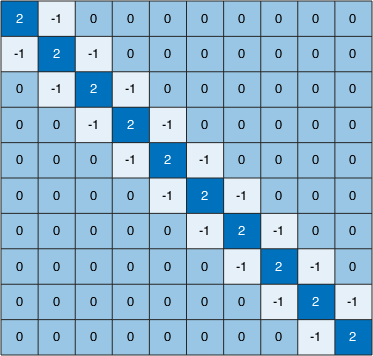
\includegraphics[height=10em]{Figures/originalmat.png}}}
\end{equation*}
}%
\only<3->{
\begin{equation*}
	T_n^{-1} = \vcenter{\hbox{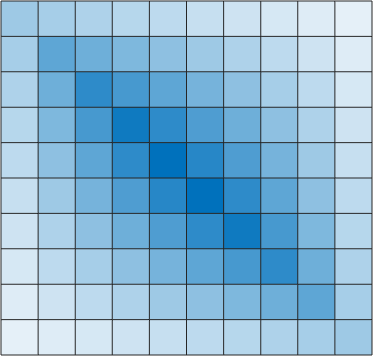
\includegraphics[height=10em]{Figures/invmat.png}}}
\end{equation*}
}
\onslide<4->{So the answer is \alert{\textbf{no}}, but$\ldots$ it seems that there is still some structure there, doesn't it?}


\end{frame}

\begin{frame}{The Gohberg--Semencul formula}
$\ldots$ starting from a \textbf{displacement representation} of $T_n$, i.e., 
\[\hspace{-1.9em}\scriptsize
t_0 T_n = \begin{bmatrix}
	t_0 & 0 & \cdots & 0 \\
	t_1 & t_0 & \ddots & \vdots \\
	\vdots & \vdots & \ddots & 0 \\
	t_{n-1} & t_{n-2} & \cdots & t_0 
\end{bmatrix}\hspace{-0.2em}\begin{bmatrix}
t_0 & t_{-1} & \cdots & t_{1-n} \\
0 & t_0 & \cdots & t_{2-n} \\
0 & 0 &  & \vdots \\
\vdots & \vdots & & t_{-1} \\
0 & 0 & \cdots & t_0
\end{bmatrix} - \begin{bmatrix}
0 & 0 & \cdots & 0  & 0 \\
t_1 & 0 & \cdots & 0 & 0 \\
t_2 & t_1 & \ddots & \vdots & \vdots \\
\vdots & \vdots & \ddots & 0 & 0 \\
t_{n-1} & t_{n-2} & \cdots & t_1 & 0
\end{bmatrix}\hspace{-0.2em}\begin{bmatrix}
0 & t_{-1} & t_{-2} & \cdots & t_{1-n} \\
0 & 0 & t_{-1} & \cdots & t_{2-n} \\
\vdots & \vdots & \vdots & \ddots & \vdots \\
0 & 0 & 0 & & t_{-1} \\
0 & 0 & 0 & \cdots & 0
\end{bmatrix}
\]
\cite{MR0353038} obtained a \textbf{displacement representation} of the \textbf{inverse}
\[\hspace{-1.9em}\scriptsize
z_1 T_n^{-1} = \begin{bmatrix}
	z_1 & 0 & \cdots & 0 \\
	z_2 & z_1 & \ddots & \vdots \\
	\vdots & \vdots & \ddots & 0 \\
	z_{n-1} & z_{n-2} & \cdots & 0 \\
	z_{n} & z_{n-1} & \cdots & z_1 
\end{bmatrix}\hspace{-0.2em}\begin{bmatrix}
	v_{n} & v_{n-1} & \cdots & v_{1} \\
	0 & v_n & \cdots & v_{2} \\
	0 & 0 &  & \vdots \\
	\vdots & \vdots & & v_{n-1} \\
	0 & 0 & \cdots & v_n
\end{bmatrix} - \begin{bmatrix}
	0 & 0 & \cdots & 0  & 0 \\
	v_1 & 0 & \cdots & 0 & 0 \\
	v_2 & v_1 & \ddots & \vdots & \vdots \\
	\vdots & \vdots & \ddots & 0 & 0 \\
	v_{n-1} & v_{n-2} & \cdots & v_1 & 0
\end{bmatrix}\hspace{-0.2em}\begin{bmatrix}
	0 & z_{n} & z_{n-1} & \cdots & z_{1} \\
	0 & 0 & z_{n} & \cdots & z_{2} \\
	\vdots & \vdots & \vdots & \ddots & \vdots \\
	0 & 0 & 0 & & z_{n} \\
	0 & 0 & 0 & \cdots & 0
\end{bmatrix}
\]
with $z_1 = v_n$.
\end{frame}

\begin{frame}{Direct Toeplitz solvers}
By cleverly computing the vectors $\mathbf{z}$ and $\mathbf{v}$ from the $\{t_n\}_n$ coefficients, one obtains several ``fast'' and ``superfast'' algorithms:
\begin{center}
\begin{tabular}{lc}
	\toprule
	Algorithm & Complexity \\
	\midrule
	\cite{levinson1946wiener} & $O(n^2)$ \\
	\cite{trench1964algorithm} & $O(n^2)$ \\
	\cite{zohar1974solution} & $O(n^2)$ \\
	\cite{bitmead1980asymptotically} & $O(n \log^2(n))$\\
	\cite{brent1980fast} & $O(n\log^2(n))$ \\
	\cite{de1987new} & $O(n\log^2(n))$ \\
	\cite{ammar1988superfast} & $O(n \log^2(n))$\\
	\cite{chan1992look} & $O(n^2)$ \\
	\midrule
	\cite{MR1685049} & $O(n \log m + m \log^2 m \log \nicefrac{n}{m})$\\
	\bottomrule
\end{tabular}

$n$ size of the matrix, $m$ size of the bandwidth.
\end{center}
\end{frame}

\begin{frame}{In our case}
To treat our case
\[
\left( I_N - \frac{\Delta t}{h_N^\alpha} \left[ \theta G_N + (1-\theta) G_N^T \right] \right) \mathbf{w}^{n+1} = \mathbf{w}^n
\]
we can then apply one of those algorithms (some of them use \emph{symmetry}).
\begin{itemize}
	\item[\faQuestionCircle]<2-> What happens if we need to treat the case
	\[
	\left( I_N - \frac{\Delta t}{h_N^\alpha} \left[ D_n^{(1)} G_N + D_n^{(2)} G_N^T \right] \right) \mathbf{w}^{n+1} = \mathbf{w}^n
	\]
	with $D_n^{(\cdot)}$ diagonal matrices coming from the discretization of \textbf{anisotropic space-variant diffusion coefficients}?
	\item[\faQuestionCircle]<3-> What happens if we need to treat \textbf{multi-dimensional cases}?
\end{itemize} 
\end{frame}

\subsection{Iterative methods for Toeplitz-like linear systems}

\begin{frame}{Krylov subspace methods}
To overcome these challenges, we use an iterative approach based on \textbf{Krylov subspaces}.

\begin{block}{Krylov subspace}
A \emph{Krylov subspace} $\mathcal{K}$ for the matrix $A$ related to
a non null vector $\mathbf{v}$ is defined as
\begin{equation*}
	\mathcal{K}_m(A,\mathbf{v})=\operatorname{Span}\{ \mathbf{v},A \mathbf{v},A^2 \mathbf{v},\ldots,A^{m-1} \mathbf{v} \}.
\end{equation*}
\end{block}

\begin{itemize}
	\item[\faExclamationCircle]<2-> The fundamental operation is the \textbf{matrix-vector} product.
	\item[\faLightbulb]<3-> Their use is \emph{effective} when these \textbf{products are cheap}.
	\item[\faMoneyBillWave]<4-> We can compute $T_n(f)\mathbf{v}$ in $O(n\log(n))$ operations!
	\[
	\hspace{-2em}C_{2n} \begin{bmatrix}
		\mathbf{v} \\
		\mathbf{0}_{n} \end{bmatrix}
	= \underbrace{\begin{bmatrix}
		T_n(f) & E_n \\
		E_n & T_n(f)
	\end{bmatrix}}_{\text{Circulant}}\begin{bmatrix}
		\mathbf{v} \\
		\mathbf{0}_{n} \end{bmatrix} = \begin{bmatrix}
		T_n(f) \mathbf{v} \\
		 E_n \mathbf{v} \end{bmatrix}, \quad     {\small E_n = \begin{bmatrix}
		0 & t_{n-1} & \ldots & t_{2} & t_{1} \\
		t_{1-n} & 0 & t_{n-1} & \ldots & t_{2}  \\
		\vdots & t_{1-n} & 0 & \ddots &  \vdots \\
		t_{-2} & \ldots & \ddots & \ddots & t_{n-1} \\
		t_{-1} & t_{-2} & \ldots & t_{1-n} & 0
	\end{bmatrix}}.
	\] 
\end{itemize}

\end{frame}

\subsection{The Conjugate Gradient Method}

\begin{frame}{The Conjugate Gradient Method}

\begin{columns}
\begin{column}{0.56\columnwidth}
When $A$ is \alert{\textbf{symmetric positive definite}} the method of choice is the \textbf{C}onjugate \textbf{G}radient.

\begin{alertblock}{Theorem.}
Let $A$ be SPD and $k_2(A)=\lambda_n/\lambda_1$ be the $2$--norm
condition number of $A$. We have:\vspace{-0.5em}
\begin{equation*}
	\frac{\|\mathbf{r}^{(m)}\|_2}{\|\mathbf{r}^{(0)}\|_2}\leq
	\sqrt{k_2(A)}
	\frac{\|\mathbf{x}^{*}-\mathbf{x}^{(m)}\|_A}{\|\mathbf{x}^{*}-\mathbf{x}^{(0)}\|_A}.
\end{equation*}
\end{alertblock}

\begin{alertblock}{Corollary.}
If $A$ is SPD with eigenvalues $0<\lambda_1\leq\ldots\leq\lambda_n$, we have\vspace{-0.5em}
\begin{equation*}
	\frac{\|\mathbf{x}^*-\mathbf{x}^{(m)}\|_A}{\|\mathbf{x}^*-\mathbf{x}^{(0)}\|_A}
	\leq 2\left ( \frac{\sqrt{k_2(A)}-1}{\sqrt{k_2(A)}+1}\right)^m.
\end{equation*}
\end{alertblock}

\end{column}
\begin{column}{0.38\columnwidth}
\begin{algorithm}[H]\scriptsize
	\KwIn{$A \in \R^{n\times n}$ SPD, $N_{max}$, $\mathbf{x}^{(0)}$}
	\KwOut{$\tilde{\mathbf{x}}$, candidate approximation.}
	$\mathbf{r}^{(0)}\leftarrow \|\mathbf{b}-A \mathbf{x}^{(0)}\|_2 $, $\mathbf{r}=\mathbf{r}^{(0)}$, $\mathbf{p}\leftarrow \mathbf{r}$\;
	$\rho_0\leftarrow\|\mathbf{r}^{(0)}\|^2$\;
	\For{$k=1,\ldots,N_{{max}}$}{
		\If{$k=1$}{
			$\mathbf{p} \leftarrow \mathbf{r}$\;
		}\Else{
			$\beta\leftarrow\nicefrac{\rho_1}{\rho_0}$\;
			$\mathbf{p}\leftarrow\mathbf{r}+\beta\, \mathbf{p}$\;
		}
		$\mathbf{w}\leftarrow A\,\mathbf{p}$\;
		$\alpha\leftarrow\nicefrac{\rho_1}{\mathbf{p}^T \mathbf{w}}$\;
		$\mathbf{x}\leftarrow \mathbf{x}+\alpha \mathbf{p}$\;
		$\mathbf{r}\leftarrow \mathbf{r}-\alpha \mathbf{w}$\;
		$\rho_1\leftarrow\|\mathbf{r}\|_2^2$\;
		\If{<Stopping criteria satisfied>}{
			\textbf{Return:} $\tilde{\mathbf{x}} = \mathbf{x}$\; 
		}
	}
\end{algorithm}
\end{column}
\end{columns}

\end{frame}

\begin{frame}{The Conjugate Gradient Method}
\alert{\faExclamationTriangle} The bound in the corollary is \textbf{descriptive} of the convergence behavior.

\begin{alertblock}{Theorem.}<2->
Let $A \in \mathbb{R}^{n \times n}$ be SPD. Let $m$ an integer,
$1<m<n$ and $c>0$ a constant such that for the eigenvalues of $A$ we
have 
$$
0<\lambda_1\leq \lambda_2\leq \lambda_3\leq \ldots \leq
\lambda_{n-m+1} \leq c < \ldots \leq \lambda_n.
$$
Fixed $\varepsilon>0$ an upper bound in exact arithmetic
for the minimum number of iterations $k$ reducing the relative error
in energy norm form the approximation $\mathbf{x}^{(k)}$ generated by CG by
$\varepsilon$ is given by
\begin{equation*}
	\min \left\{ \left\lceil \frac12 \sqrt{c/\lambda_1} \log{\left(
		\frac{2}{\varepsilon} \right)}+m+1\right\rceil,n \right\}
\end{equation*}
\end{alertblock}

\onslide<3>{\faQuestionCircle\; How can we put ourselves in the hypotheses of the Theorem?}

\end{frame}

\begin{frame}{Clustered spectra}

\begin{block}{A proper cluster}
	    A sequence of matrices $\{A_n\}_{n \geq 0}$, $A_n \in
	\mathbb{C}^{n \times
		n}$, has a \textbf{proper cluster} of eigenvalues in $p \in
	\mathbb{C}$
	if, $\forall \varepsilon > 0$, if the number of eigenvalues of
	$A_n$
	\textbf{not in} $D(p,\varepsilon) = \{z \in \mathbb{C}\,|\;
	|z-p|<\varepsilon\}$ is
	bounded by a constant $r$ that does not depend on $n$. Eigenvalues
	not in the \emph{proper cluster} are called \textbf{outlier}
	eigenvalues.
\end{block}

\begin{itemize}
	\item[\faQuestionCircle]<2-> Do the matrices
	\[
	A_N = I_N - \frac{\Delta t}{2 h_N^\alpha} \left[ G_N + G_N^T \right]
	\]
	have a \textbf{clustered spectra}?
	\item[\faEye]<3-> We can investigate this question by looking again at the \alert{\textbf{spectral distribution}} of the sequence $\{A_N\}_N$.
\end{itemize}

\end{frame}

\begin{frame}{Asymptotic distribution: the symmetric case}\vspace{-0.5em}
	\[
A_N = I_N - \frac{\Delta t}{2 h_N^\alpha} \left[ G_N + G_N^T \right],
\]
the sequence $\{A_N\}_N$ is \textbf{not} yet \textbf{ready} for the \textbf{analysis}, we have the coefficient $\nicefrac{\Delta t}{2 h_N^\alpha}$ that varies with $N$.
\begin{itemize}
	\item[\faExclamationCircle] For \emph{consistency} reason it makes sense to select $\Delta t \equiv h_N \equiv \nu_N$, then, since $\alpha \in (1,2]$ we have that $\nu^{1-\alpha}$ for $\nu \rightarrow 0^+$ goes to $+\infty$.
	\item[$\Rightarrow$]<2-> We look instead at the sequence:
	\[
	\{ \nu_N^{\alpha-1} A_N \}_N = \{ \nu_N^{\alpha-1}I_N - \nicefrac{(G_N + G_N^T)}{2}  \}_N,
	\]
	and is such that $\|\nu^{\alpha-1} I_N\| = \nu^{\alpha-1} < C$ independently of $N$.
	\item[\faArrowCircleUp]<3-> $\{ -\nicefrac{(G_N + G_N^T)}{2} \}_N$ is now a \emph{symmetric} Toeplitz sequence with \textbf{known generating function}:
	\[
	p_\alpha(\theta) = f(\theta) + f(-\theta) = -e^{-i\theta}(1-e^{i\theta})^\alpha - e^{i\theta}(1-e^{-i\theta})^\alpha.
	\]
	\item[$\Rightarrow$]<4-> We have just discovered that: $\{\nu_N^{\alpha-1} A_N\}_N \sim_\lambda p_\alpha(\theta)$.
\end{itemize}

\end{frame}

\begin{frame}[fragile]{Asymptotic distribution: the symmetric case}\vspace{-1em}
\[
\{ \nu_N^{\alpha-1} A_N\} = \left\lbrace \nu_N^{\alpha-1} I_N - \frac{1}{2} \left[ G_N + G_N^T \right] \right\rbrace_N \sim_\lambda p_\alpha(\theta) = -e^{-i\theta}(1-e^{i\theta})^\alpha - e^{i\theta}(1-e^{-i\theta})^\alpha,
\]

\begin{columns}
\begin{column}{0.55\columnwidth}
\definecolor{bg}{rgb}{0.95,0.95,0.95}
\begin{minted}[bgcolor=bg,fontsize=\small,breaklines]{matlab}
N = 100; alpha = 1.3;
hN = 1/(N-1); dt = hN; nu = dt;
G = glmatrix(N,alpha); I = eye(N,N);
A = nu^(alpha-1)*I-0.5*(G+G');
ev = eig(A);
f = @(t)-exp(-1i*t).*(1-exp(1i*t)) .^alpha;
p = @(t)nu^(alpha-1)+0.5*(f(t) +conj(f(t)));
t = linspace(-pi,pi,N);
plot(t,ev,'o',t,sort(p(t),'ascend'),'-')
\end{minted}
\end{column}
\begin{column}{0.45\columnwidth}\centering
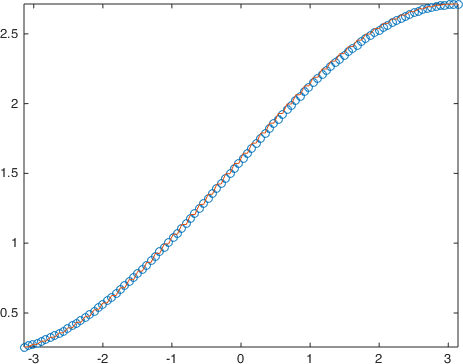
\includegraphics[width=0.8\columnwidth]{Figures/spectrumsym.png}

\onslide<2>{\alert{\faExclamationTriangle} the spectrum is \textbf{not clustered}!}
\end{column}
\end{columns}

\end{frame}

\begin{frame}[fragile]{CG with a non clustered spectra}

Let us test the CG with different values of $\alpha$ and $N$.\\[0.5em]

\begin{columns}
\begin{column}{0.4\columnwidth}
\centering

\begin{tabular}{rrrr}
	\toprule
	$\alpha$	& 1.8 & 1.5 & 1.2 \\
	\midrule
	$N$ & \multicolumn{3}{c}{Iteration} \\
	\midrule
	100 & 49 & 34 & 16\\
	200 & 87  & 42 & 17 \\
	500 & 155 & 53 & 18\\
	1000 & 209 & 63 & 19 \\
	5000 & 398 & 92 & 21\\
	10000 & 523 & 108 & 22\\
	\bottomrule
\end{tabular}
\end{column}
\begin{column}{0.6\columnwidth}
\begin{itemize}
	\item[\faEye] The number if iterations grows with $N$,
	\item[\faEye] Smaller values of $\alpha$ seem to be easier.
	\item[\faAward]<2-> We would like \textbf{number of iterations} \alert{independent} on both \alert{\textbf{size}} and value of \alert{$\alpha$}.
	In this case this is called having a method with a \textbf{superlinear convergence} and \textbf{robust with respect to the parameters}.
	\item[\faQuestionCircle]<3-> Can we?
\end{itemize}
\end{column}
\end{columns}
\definecolor{bg}{rgb}{0.95,0.95,0.95}
\begin{minted}[bgcolor=bg,fontsize=\small,breaklines]{matlab}
A = nu^(alpha-1)*I-0.5*(G+G'); b = nu^(alpha-1)*ones(N,1);
[x,flag,relres,iter,resvec] = pcg(A,b,1e-6,N)
\end{minted}

\end{frame}

\subsection{Preconditioned Conjugate Gradient}

\begin{frame}{Preconditioned CG}
\begin{columns}
\begin{column}{0.5\columnwidth}
\begin{itemize}
	\item[\faWrench] To try and achieve this result we need to \emph{modify the spectrum of the system}, i.e., we need to \alert{\textbf{precondition}}.
	\item[\faLightbulb]<2-> We modify the system
	\[
	A \mathbf{x} = \mathbf{b},
	\]
	into
	\[
	M^{-1} A \mathbf{x} = M^{-1} \mathbf{b},
	\]
	with $M$ SPD and such that $M^{-1}A$ has a \textbf{clustered spectra}.
\end{itemize}
\end{column}
\begin{column}{0.5\columnwidth}\onslide<2->{
\begin{algorithm}[H]\scriptsize
	\KwIn{$A \in \R^{n\times n}$ SPD, $N_{max}$, $\mathbf{x}^{(0)}$, $M \in \mathbb{R}^{n\times n}$ SPD preconditioner}
	$\mathbf{r}^{(0)} \leftarrow \mathbf{b}-A\mathbf{x}^{(0)}$,
	$\textbf{z}^{(0)} \leftarrow M^{-1}\mathbf{r}^{(0)}$,
	$\mathbf{p}^{(0)} \leftarrow \mathbf{z}^{(0)}$\;
	\For{$j=0,\ldots,N_{\text{max}}$}{
		$\alpha_j \leftarrow \nicefrac{<\mathbf{r}^{(j)},\mathbf{z}^{(j)}>}{A\mathbf{p}^{(j)},\mathbf{p}^{(j)}}$\;
		$\mathbf{x}^{(j+1)} \leftarrow \mathbf{x}^{(j)} + \alpha_j \mathbf{p}^{(j)}$\;
		$\mathbf{r}^{(j+1)} \leftarrow \mathbf{r}^{(j)} - \alpha_j A \mathbf{p}^{(j)}$\;
		\If{<Stopping criteria satisfied>}{
			\textbf{Return:} $\tilde{\mathbf{x}} = \mathbf{x}^{(j+1)}$\;
		}
		$\mathbf{z}^{(j+1)} \leftarrow \alert<2-3>{M^{-1} \mathbf{r}^{(j+1)}}$\;
		$\beta_{j} \leftarrow \nicefrac{<\mathbf{r}^{(j+1)},\mathbf{z}^{(j+1)}>}{<\mathbf{r}^{(j)},\mathbf{z}^{(j)}>}$\;
		$\mathbf{p}^{(j+1)} \leftarrow \mathbf{z}^{(j+1)}+\beta_j \mathbf{p}^{(j)}$\;
	}
\end{algorithm}}
\end{column}
\end{columns}
\vfill

\onslide<3>{\alert{\textbf{\faExclamationTriangle}} $M^{-1}$ has to be easy to apply, possibly it has to have the \emph{same cost of multiplying by~$A$}.}
\end{frame}

\begin{frame}{Circulant preconditioners for Toeplitz matrices}

\textcolor{yellow}{\faLightbulb} If $M$ is \alert{circulant} than applying $M^{-1}$ costs $O(n \log n)$ operations, same as applying $A$.

\onslide<2->{\faEye\,Observe that, nevertheless, this \textbf{doubles the cost per iteration}, can we do better?}

\begin{block}<3->{$\omega$-circulant matrices}
Let $\omega = \exp(i\theta)$ for $\theta \in [-\pi,\pi]$. A matrix
$W_n^{(\omega)}$ of size $n$ is said to be an \textbf{$\omega$--circulant
	matrix} if it has the spectral
decomposition \begin{equation*}
	W_n^{(\omega)} = \Omega_n^H F_n^H \Lambda_n F_n \Omega_n,
\end{equation*}
where $F_n$ is the Fourier matrix and $\Omega_n =
\operatorname{diag}(1,\omega^{\nicefrac{-1}{n}},\ldots,\omega^{\nicefrac{-(n-1)}{n}})$
and $\Lambda_n$ is the diagonal matrix of the eigenvalues. In
particular $1$--circulant matrices are circulant matrices while
$\{-1\}$--circulant matrices are the skew--circulant matrices.
\end{block}

\onslide<4->{\faLightbulb[regular] We can use them to reduce the overall cost of the preconditioning step!}

\end{frame}

\begin{frame}{Circulant preconditioners for Toeplitz matrices}

The \alert{\faKey\,key idea} is observing that we can decompose any Toeplitz matrix into the \textbf{sum of a circulant and of a skew-circulant matrix}
\begin{equation*}
	T_n = U_n + V_n, \; U_n = F_n^H \Lambda_n^{(1)} F_n, \; V_n = \Omega_n^H F_n^H \Lambda_n^{(2)} F_n \Omega_n
\end{equation*}
where
\begin{equation*}
	\begin{split}
		\mathbf{e}_1^T U_n = & \nicefrac{1}{2}\left[
		t_0 , t_{-1} + t_{n-1} , \ldots , t_{-(n-1)+t_1}
		\right],\\
		W_n\mathbf{e}_1 = & \nicefrac{1}{2}\left[
		t_0 , -(t_{n-1}-t_{-1}) , \ldots , -(t_{-1}-t_{n-1})
		\right]^T.
	\end{split}
\end{equation*}
\onslide<2->{
Then we can compute the product
\begin{equation*}
	\begin{split}
		C_n^{-1}T_n = \only<2>{\,& C_n^{-1}\left(U_n + V_n\right) = C_n^{-1}\left(F_n^H \Lambda_n^{(1)} F_n + \Omega_n^H F_n^H \Lambda_n^{(2)} F_n \Omega_n\right) \\
		=\,& F_n^H \Lambda_n^{-1} F_n\left(F_n^H \Lambda_n^{(1)} F_n + \Omega_n^H F_n^H \Lambda_n^{(2)} F_n \Omega_n\right) \\
		=\,&} F_n^H\left[\Lambda_n^{-1} \left(\Lambda_n^{(1)} + F_n \Omega_n^H F_n^H \Lambda_n^{(2)} F_n \Omega_n F_n^H \right)
		\right]F_n.
	\end{split}
\end{equation*}
}\only<3->{
And solve $C_n^{-1}T_n \mathbf{x} = C_n^{-1}\mathbf{b}$ as
\begin{equation*}
	\Lambda_n^{-1} \left(\Lambda_n^{(1)} + F_n \Omega_n^H F_n^H
	\Lambda_n^{(2)} F_n \Omega_n F_n^H \right) \underbrace{F_n
		\mathbf{x}}_{= \tilde{\mathbf{x}}} = \underbrace{\Lambda_n^{-1} F_n
		\mathbf{b}}_{= \tilde{\mathbf{b}}} \onslide<4->{ \text{ \alert{4 FFTs per iteration!}} }
\end{equation*}
}

\end{frame}

\begin{frame}{Circulant preconditioners for Toeplitz matrices}
\faQuestionCircle\,This is then \emph{computationally efficient}, can we find the right circulant matrix to have a clustered spectra?

\onslide<2->{\alert{\faWrench}\,We need to change the problem into an equivalent one: the aim is \textbf{discharging everything on the generating functions}!}

\only<3>{
\begin{block}{Continuous convolution}
Given two scalar functions $f$ and $g$ in the Schwartz space, i.e.,
$f,g \in \mathcal{C}^{\infty}(\mathbb{R})$ such that $\exists\,
C_{\alpha,\beta}^{(f)},  C_{\alpha',\beta'}^{(g)} \in \mathbb{R}$
with $\|x^{\alpha} \partial_\beta f(x)\|_{\infty} \leq
C^{\alpha\beta}$ and $\|x^{\alpha'} \partial_{\beta'}
g(x)\|_{\infty} \leq C^{\alpha'\beta'}$, $\alpha$, $\beta$, $\alpha'$,
$\beta'$ scalar indices, we define the \textbf{convolution
	operation}, ``$*$'', as
\begin{equation*}
	[f*g](t) = \int_{-\infty}^{+\infty}f(\tau)g(t-\tau)d\,\tau =
	\int_{-\infty}^{+\infty} g(\tau)f(t-\tau)d\,\tau.
\end{equation*}
\end{block}}
\only<4>{\begin{block}<4->{Discrete convolution}
For two arbitrary $2\pi$--periodic continuous functions,
\begin{equation*}
	f(\theta) = \sum_{k=-\infty}^{+\infty} t_k e^{ik\theta} \text{ and } g = \sum_{k=-\infty}^{+\infty} s_k e^{ik\theta}
\end{equation*}
their \textbf{convolution product} is given by
\begin{equation*}
	[f*g](\theta) = \sum_{k=-\infty}^{+\infty} s_k t_k e^{ik\theta}.
\end{equation*}
\end{block}}
\only<5->{
\begin{exampleblock}{\faLightbulb\,Using a Kernel}
Given a kernel $\mathcal{K}_n(\theta)$ defined on $[0,2\pi]$
and a generating function $f$ for a Toeplitz sequence $T_n(f)$, we
consider the circulant matrix $C_n$ with eigenvalues given by
\begin{equation*}
	\lambda_j(C_n) = \left[ \mathcal{K}_n * f \right] \left(\frac{2\pi j}{n}\right), 0 \leq j < n,
\end{equation*}
\end{exampleblock}

\begin{itemize}
	\item[\faLightbulb]<6-> We have rewritten the problem of \textbf{finding an appropriate preconditioner} to the problem of \textbf{approximating the generating
	function} of the underlying Toeplitz matrix.
\end{itemize}

}
\end{frame}

\begin{frame}{Circulant preconditioners for Toeplitz matrices}

\begin{alertblock}{Theorem \parencite{MR1173187}}
Lef $f$ be a $2\pi$--periodic \alert<2>{continuous positive function}. Let
$\mathcal{K}_n(\theta)$ be a kernel such that $\mathcal{K}_n * f
\overset{n \rightarrow +\infty}{\longrightarrow} f$ uniformly on
$[-\pi,\pi]$. If $C_n$ is the sequence of circulant matrices with
eigenvalues given by
\[
\lambda_j(C_n) = \left[ \mathcal{K}_n * f \right] \left(\frac{2\pi j}{n}\right), 0 \leq j < n,
\]
then the spectra of the sequence $\{C_n^{-1}T_n(f)\}_n$ is clustered
around $1$.
\end{alertblock}

\begin{itemize}
	\item[\faQuestionCircle] Is this the result we need?
	\item[\faExclamationCircle]<2> It requires a \emph{continuous positive function} generating function $f$! Ours is:
	\[
	 p_\alpha(\theta) = -e^{-i\theta}(1-e^{i\theta})^\alpha - e^{i\theta}(1-e^{-i\theta})^\alpha,
	\]
	and it does seem to have a zero.
\end{itemize}

\end{frame}

\begin{frame}{Circulant preconditioners: cases with a zero}

\begin{block}{Order of the zero}
Let $f:[a,b] \subset \mathbb{R} \rightarrow \mathbb{R}$ be a continuous nonnegative function. We say that $f$ has a zero order $\beta > 0$ at $\theta_0 \in [a,b]$ if there exist two real constants $C_1,C_2 > 0$ such that
\[
\liminf_{\theta \rightarrow \theta_0} \frac{f(\theta)}{|\theta - \theta_0|^\beta} = C_1, \quad \limsup_{\theta \rightarrow \theta_0} \frac{f(\theta)}{|\theta - \theta_0|^\beta} = C_2.
\]
\end{block}

\begin{alertblock}<2->{Proposition \parencite{MR3448208}}
Given $\alpha \in (1,2)$, then the function $p_\alpha(\theta)$ is nonnegative and has a zero of order $\alpha$ at $0$.
\end{alertblock}

\onslide<3->{\textbf{Proof.} \only<3->{We first prove that is nonnegative by direct computation
\[
p_\alpha(\theta) = \only<3>{- \sum_{k=-1}^{+\infty} g_{k+1}^{(\alpha)}(e^{ik\theta} + e^{-ik\theta})} \only<4>{- \left[ 2g_1^{(\alpha)} + (g_0^{(\alpha)} + g_2^{(\alpha)})(e^{i\theta} + e^{-i\theta}) + \sum_{k=2}^{+\infty} g_{k+1}^{(\alpha)} (e^{ik\theta} + e^{-ik\theta})  \right]} \only<5->{- \left[ 2g_1^{(\alpha)} + 2(g_0^{(\alpha)} + g_2^{(\alpha)})\cos\theta + 2\sum_{k=2}^{+\infty} g_{k+1}^{(\alpha)} cos(k\theta)  \right]} \only<6->{ \geq - 2 \sum_{k=-1}^{+\infty} g_{k+1}^{(\alpha)} = 0. } 
\]
}
}

\end{frame}

\begin{frame}{Circulant preconditioners: cases with a zero}
\begin{alertblock}{Proposition \parencite{MR3448208}}
	Given $\alpha \in (1,2)$, then the function $p_\alpha(\theta)$ is nonnegative and has a zero of order $\alpha$ at $0$.
\end{alertblock}

\textbf{Proof.} Then we focus on the zero. Let us rewrite
\[
1 - e^{i\theta} = \sqrt{2-2\cos\theta} e^{i\phi}, \quad 1 - e^{-i\theta} = \sqrt{2-2\cos\theta}e^{i\psi},
\]
\only<1>{where
\[
\phi = \begin{cases}
	\arctan \left( \frac{- \sin\theta}{1-\cos\theta} \right), & \theta \neq 0,\\
	\lim_{\theta \rightarrow 0^+} \arctan \left( \frac{- \sin\theta}{1-\cos\theta} \right) = - \frac{\pi}{2}, & \theta = 0.
\end{cases} \quad \psi = -\phi.
\]}\only<2>{
and write
\[
\begin{split}
p_\alpha(\theta) = & - e^{-i\theta} ( \sqrt{2-2\cos\theta} e^{i\phi} )^\alpha - e^{i\theta} ( \sqrt{2-2\cos\theta} e^{-i\phi} )^\alpha \\
= & - \sqrt{(2 - 2\cos\theta)^\alpha} e^{i(\alpha \phi - \theta)} - \sqrt{(2-2\cos\theta)^\alpha} e^{-i(\alpha\phi - \theta)} \\
= & -2 \sqrt{(2-2\cos\theta)^\alpha}r_\alpha(\theta), \qquad r_\alpha(\theta) = \cos(\alpha \phi - \theta).
\end{split}
\]
}
\only<3>{
and write
\[
\begin{split}
	p_\alpha(\theta) = -2 \sqrt{(2-2\cos\theta)^\alpha}r_\alpha(\theta), \qquad r_\alpha(\theta) = \cos(\alpha \phi - \theta).
\end{split}
\]
Since $\displaystyle \lim_{\theta \rightarrow 0^{-}} r_\alpha(\theta) = \lim_{\theta \rightarrow 0^{+}} r_\alpha(\theta) = \cos(\alpha \nicefrac{\pi}{2})$, we find
\[
\lim_{\theta \rightarrow 0} \frac{p_\alpha(\theta)}{|\theta|^\alpha} = - 2 \lim_{\theta \rightarrow 0} \frac{(2-2\cos\theta)^{\nicefrac{\alpha}{2}}}{|\theta|^\alpha} r_\alpha(\theta) = - 2 \cos (\alpha \nicefrac{\pi}{2}) \in (0,2),
\]
i.e., $p_\alpha$ has a zero of order $\alpha$ at $0$ according to the definition. \hfil \qedsymbol
}
\end{frame}

\begin{frame}[fragile]{Circulant preconditioners: cases with a zero}

\begin{columns}
\begin{column}{0.5\columnwidth}
\begin{onlyenv}<1>
\definecolor{bg}{rgb}{0.95,0.95,0.95}
\begin{minted}[bgcolor=bg,fontsize=\small,breaklines]{matlab}
t = linspace(-pi,pi,100);
f = @(alpha) -exp(-1i*t).*(1-exp(1i*t)).^alpha;
p = @(alpha) f(alpha) + conj(f(alpha));
plot(t,p(1.2)./max(p(1.2)),...
 t,p(1.5)./max(p(1.5)),...
 t,p(1.8)./max(p(1.8)),
 t,p(2)./max(p(2)),...
 'LineWidth',2);
legend({'\alpha=1.2','\alpha=1.5',...
 '\alpha=1.8','\alpha=2'},...
 'Location','north');
\end{minted}
\end{onlyenv}%
\only<2->{
\begin{itemize}
\item[\faEye] $p_2(\theta)	= 2(2-2\cos\theta)$, i.e., $2 \times $Laplacian generating function,
\item[\faEye] $p_\alpha(\theta)/\|p_\alpha\|_\infty$ \alert{approaches the order of the zero of the Laplacian} in $0$, i.e., it increases up to $2$ as $\alpha$ tends to 2. 
\item[\faQuestionCircle]<3-> What can we do for the case in this case?
\item[\faLightbulb]<4-> \textbf{matching the zeros} of the generating function, \emph{heuristically}, if the preconditioner have a spectrum that behaves as a function $g$ with zeros of the same order, and in the same place of $f$, then $f/g$ no loner have the problematic behavior$\ldots$ 
\end{itemize}
}
\end{column}
\begin{column}{0.5\columnwidth}
\centering	
	
\only<1>{% This file was created by matlab2tikz.
%
%The latest updates can be retrieved from
%  http://www.mathworks.com/matlabcentral/fileexchange/22022-matlab2tikz-matlab2tikz
%where you can also make suggestions and rate matlab2tikz.
%
\definecolor{mycolor1}{rgb}{0.00000,0.44700,0.74100}%
\definecolor{mycolor2}{rgb}{0.85000,0.32500,0.09800}%
\definecolor{mycolor3}{rgb}{0.92900,0.69400,0.12500}%
\definecolor{mycolor4}{rgb}{0.49400,0.18400,0.55600}%
%
\begin{tikzpicture}

\begin{axis}[%
width=0.8\columnwidth,
height=0.8\columnwidth,
at={(0.758in,0.481in)},
scale only axis,
xmin=-3.14159265358979,
xmax=3.14159265358979,
xtick={-3.14159265358979,-1.5707963267949,0,1.5707963267949,3.14159265358979},
xticklabels={{$\text{-}\pi$},{$\text{-}\pi\text{/2}$},{0},{$\pi\text{/2}$},{$\pi$}},
ymin=0.000251728808407433,
ymax=1,
axis background/.style={fill=white},
legend style={at={(0.5,0.97)}, anchor=north, legend cell align=left, align=left, draw=none}
]
\addplot [color=mycolor1, line width=2.0pt]
  table[row sep=crcr]{%
-3.14159265358979	1\\
-3.07812613533545	0.999073853331874\\
-3.01465961708111	0.996298928477964\\
-2.95119309882678	0.991685756614505\\
-2.88772658057244	0.985251842174874\\
-2.8242600623181	0.977021591757801\\
-2.76079354406376	0.967026214995518\\
-2.69732702580942	0.955303597776579\\
-2.63386050755508	0.941898148328065\\
-2.57039398930074	0.926860616769934\\
-2.5069274710464	0.9102478888597\\
-2.44346095279206	0.892122754748302\\
-2.37999443453772	0.872553653667239\\
-2.31652791628338	0.851614395562724\\
-2.25306139802904	0.829383860784106\\
-2.1895948797747	0.805945679021016\\
-2.12612836152037	0.78138788876613\\
-2.06266184326603	0.755802578658012\\
-1.99919532501169	0.729285512130836\\
-1.93572880675735	0.701935736864879\\
-1.87226228850301	0.673855180593343\\
-1.80879577024867	0.645148234877471\\
-1.74532925199433	0.615921328513083\\
-1.68186273373999	0.586282492278134\\
-1.61839621548565	0.556340916773168\\
-1.55492969723131	0.526206505145659\\
-1.49146317897697	0.49598942252679\\
-1.42799666072263	0.46579964404741\\
-1.36453014246829	0.435746503342254\\
-1.30106362421395	0.40593824350312\\
-1.23759710595962	0.376481572510374\\
-1.17413058770528	0.347481225269643\\
-1.11066406945094	0.319039534525236\\
-1.0471975511966	0.291256013142191\\
-0.983731032942258	0.264226950590739\\
-0.920264514687919	0.23804502700492\\
-0.85679799643358	0.212798949045603\\
-0.793331478179241	0.188573113190934\\
-0.729864959924901	0.165447304381708\\
-0.666398441670562	0.143496441856349\\
-0.602931923416223	0.122790390836153\\
-0.539465405161884	0.10339387109286\\
-0.475998886907544	0.085366516887868\\
-0.412532368653205	0.0687631898041519\\
-0.349065850398866	0.053634747146473\\
-0.285599332144527	0.0400297067081271\\
-0.222132813890187	0.0279978810985922\\
-0.158666295635848	0.0175990468306273\\
-0.0951997773815089	0.00892791129364437\\
-0.0317332591271696	0.00222408370274357\\
0.0317332591271696	0.00222408370274357\\
0.0951997773815089	0.00892791129364437\\
0.158666295635848	0.0175990468306273\\
0.222132813890187	0.0279978810985922\\
0.285599332144527	0.0400297067081271\\
0.349065850398866	0.053634747146473\\
0.412532368653205	0.0687631898041519\\
0.475998886907544	0.085366516887868\\
0.539465405161884	0.10339387109286\\
0.602931923416223	0.122790390836153\\
0.666398441670562	0.143496441856349\\
0.729864959924901	0.165447304381708\\
0.793331478179241	0.188573113190934\\
0.85679799643358	0.212798949045603\\
0.920264514687919	0.23804502700492\\
0.983731032942258	0.264226950590739\\
1.0471975511966	0.291256013142191\\
1.11066406945094	0.319039534525236\\
1.17413058770528	0.347481225269643\\
1.23759710595962	0.376481572510374\\
1.30106362421395	0.40593824350312\\
1.36453014246829	0.435746503342254\\
1.42799666072263	0.46579964404741\\
1.49146317897697	0.49598942252679\\
1.55492969723131	0.526206505145659\\
1.61839621548565	0.556340916773168\\
1.68186273373999	0.586282492278134\\
1.74532925199433	0.615921328513083\\
1.80879577024867	0.645148234877471\\
1.87226228850301	0.673855180593343\\
1.93572880675735	0.701935736864879\\
1.99919532501169	0.729285512130836\\
2.06266184326603	0.755802578658012\\
2.12612836152037	0.78138788876613\\
2.1895948797747	0.805945679021016\\
2.25306139802904	0.829383860784106\\
2.31652791628338	0.851614395562724\\
2.37999443453772	0.872553653667239\\
2.44346095279206	0.892122754748302\\
2.5069274710464	0.9102478888597\\
2.57039398930074	0.926860616769934\\
2.63386050755508	0.941898148328065\\
2.69732702580942	0.955303597776579\\
2.76079354406376	0.967026214995518\\
2.8242600623181	0.977021591757801\\
2.88772658057244	0.985251842174874\\
2.95119309882678	0.991685756614505\\
3.01465961708111	0.996298928477964\\
3.07812613533545	0.999073853331874\\
3.14159265358979	1\\
};
\addlegendentry{$\alpha\text{=1.2}$}

\addplot [color=mycolor2, line width=2.0pt]
  table[row sep=crcr]{%
-3.14159265358979	1\\
-3.07812613533545	0.999119131352826\\
-3.01465961708111	0.996479597322377\\
-2.95119309882678	0.992090602110462\\
-2.88772658057244	0.985967447664733\\
-2.8242600623181	0.978131476268114\\
-2.76079354406376	0.968609990508562\\
-2.69732702580942	0.957436150972645\\
-2.63386050755508	0.944648852103188\\
-2.57039398930074	0.93029257675691\\
-2.5069274710464	0.914417230092498\\
-2.44346095279206	0.897077953512761\\
-2.37999443453772	0.878334919476343\\
-2.31652791628338	0.858253108084927\\
-2.25306139802904	0.836902066441001\\
-2.1895948797747	0.81435565185932\\
-2.12612836152037	0.790691760102445\\
-2.06266184326603	0.765992039897731\\
-1.99919532501169	0.740341595080557\\
-1.93572880675735	0.713828675797451\\
-1.87226228850301	0.686544360294492\\
-1.80879577024867	0.658582228912786\\
-1.74532925199433	0.630038032016504\\
-1.68186273373999	0.601009353693371\\
-1.61839621548565	0.57159527319718\\
-1.55492969723131	0.541896026253271\\
-1.49146317897697	0.512012668529407\\
-1.42799666072263	0.482046743798106\\
-1.36453014246829	0.45209995959857\\
-1.30106362421395	0.422273873570129\\
-1.23759710595962	0.392669594107575\\
-1.17413058770528	0.363387499629563\\
-1.11066406945094	0.334526981624435\\
-1.0471975511966	0.306186217847897\\
-0.983731032942258	0.278461983753209\\
-0.920264514687919	0.251449512684521\\
-0.85679799643358	0.225242418952323\\
-0.793331478179241	0.199932703282025\\
-0.729864959924901	0.175610868370841\\
-0.666398441670562	0.152366185302966\\
-0.602931923416223	0.130287172804112\\
-0.539465405161884	0.109462387308051\\
-0.475998886907544	0.0899816856773844\\
-0.412532368653205	0.071938242210594\\
-0.349065850398866	0.0554318421447268\\
-0.285599332144527	0.0405745009281765\\
-0.222132813890187	0.0275007539853635\\
-0.158666295635848	0.0163887025821987\\
-0.0951997773815089	0.00751176313462669\\
-0.0317332591271696	0.00142430466603073\\
0.0317332591271696	0.00142430466603073\\
0.0951997773815089	0.00751176313462669\\
0.158666295635848	0.0163887025821987\\
0.222132813890187	0.0275007539853635\\
0.285599332144527	0.0405745009281765\\
0.349065850398866	0.0554318421447268\\
0.412532368653205	0.071938242210594\\
0.475998886907544	0.0899816856773844\\
0.539465405161884	0.109462387308051\\
0.602931923416223	0.130287172804112\\
0.666398441670562	0.152366185302966\\
0.729864959924901	0.175610868370841\\
0.793331478179241	0.199932703282025\\
0.85679799643358	0.225242418952323\\
0.920264514687919	0.251449512684521\\
0.983731032942258	0.278461983753209\\
1.0471975511966	0.306186217847897\\
1.11066406945094	0.334526981624435\\
1.17413058770528	0.363387499629563\\
1.23759710595962	0.392669594107575\\
1.30106362421395	0.422273873570129\\
1.36453014246829	0.45209995959857\\
1.42799666072263	0.482046743798106\\
1.49146317897697	0.512012668529407\\
1.55492969723131	0.541896026253271\\
1.61839621548565	0.57159527319718\\
1.68186273373999	0.601009353693371\\
1.74532925199433	0.630038032016504\\
1.80879577024867	0.658582228912786\\
1.87226228850301	0.686544360294492\\
1.93572880675735	0.713828675797451\\
1.99919532501169	0.740341595080557\\
2.06266184326603	0.765992039897731\\
2.12612836152037	0.790691760102445\\
2.1895948797747	0.81435565185932\\
2.25306139802904	0.836902066441001\\
2.31652791628338	0.858253108084927\\
2.37999443453772	0.878334919476343\\
2.44346095279206	0.897077953512761\\
2.5069274710464	0.914417230092498\\
2.57039398930074	0.93029257675691\\
2.63386050755508	0.944648852103188\\
2.69732702580942	0.957436150972645\\
2.76079354406376	0.968609990508562\\
2.8242600623181	0.978131476268114\\
2.88772658057244	0.985967447664733\\
2.95119309882678	0.992090602110462\\
3.01465961708111	0.996479597322377\\
3.07812613533545	0.999119131352826\\
3.14159265358979	1\\
};
\addlegendentry{$\alpha\text{=1.5}$}

\addplot [color=mycolor3, line width=2.0pt]
  table[row sep=crcr]{%
-3.14159265358979	1\\
-3.07812613533545	0.999073837114462\\
-3.01465961708111	0.996298669352665\\
-2.95119309882678	0.991684447772029\\
-2.88772658057244	0.985247718757887\\
-2.8242600623181	0.97701156612034\\
-2.76079354406376	0.967005530354192\\
-2.69732702580942	0.95526550538534\\
-2.63386050755508	0.941833613217955\\
-2.57039398930074	0.926758056986782\\
-2.5069274710464	0.910092953007674\\
-2.44346095279206	0.891898142506917\\
-2.37999443453772	0.872238983795905\\
-2.31652791628338	0.851186125742185\\
-2.25306139802904	0.828815263470862\\
-2.1895948797747	0.805206877311807\\
-2.12612836152037	0.780445956088309\\
-2.06266184326603	0.754621705921922\\
-1.99919532501169	0.727827245806786\\
-1.93572880675735	0.700159291285166\\
-1.87226228850301	0.671717827635211\\
-1.80879577024867	0.642605774063183\\
-1.74532925199433	0.612928640477042\\
-1.68186273373999	0.582794178508545\\
-1.61839621548565	0.552312028549496\\
-1.55492969723131	0.521593364678394\\
-1.49146317897697	0.490750539481321\\
-1.42799666072263	0.45989673092251\\
-1.36453014246829	0.429145593604878\\
-1.30106362421395	0.39861091699204\\
-1.23759710595962	0.368406293459098\\
-1.17413058770528	0.338644799425836\\
-1.11066406945094	0.309438693340184\\
-1.0471975511966	0.280899134976805\\
-0.983731032942258	0.253135931477369\\
-0.920264514687919	0.22625731691025\\
-0.85679799643358	0.200369774062937\\
-0.793331478179241	0.175577910011915\\
-0.729864959924901	0.151984401255623\\
-0.666398441670562	0.129690030720218\\
-0.602931923416223	0.108793849300173\\
-0.539465405161884	0.0893935116298297\\
-0.475998886907544	0.0715858650476828\\
-0.412532368653205	0.0554679236939393\\
-0.349065850398866	0.0411384619894574\\
-0.285599332144527	0.0287006762132623\\
-0.222132813890187	0.0182668639284931\\
-0.158666295635848	0.0099674325885581\\
-0.0951997773815089	0.00397121543737497\\
-0.0317332591271696	0.000548897595548665\\
0.0317332591271696	0.000548897595548665\\
0.0951997773815089	0.00397121543737497\\
0.158666295635848	0.0099674325885581\\
0.222132813890187	0.0182668639284931\\
0.285599332144527	0.0287006762132623\\
0.349065850398866	0.0411384619894574\\
0.412532368653205	0.0554679236939393\\
0.475998886907544	0.0715858650476828\\
0.539465405161884	0.0893935116298297\\
0.602931923416223	0.108793849300173\\
0.666398441670562	0.129690030720218\\
0.729864959924901	0.151984401255623\\
0.793331478179241	0.175577910011915\\
0.85679799643358	0.200369774062937\\
0.920264514687919	0.22625731691025\\
0.983731032942258	0.253135931477369\\
1.0471975511966	0.280899134976805\\
1.11066406945094	0.309438693340184\\
1.17413058770528	0.338644799425836\\
1.23759710595962	0.368406293459098\\
1.30106362421395	0.39861091699204\\
1.36453014246829	0.429145593604878\\
1.42799666072263	0.45989673092251\\
1.49146317897697	0.490750539481321\\
1.55492969723131	0.521593364678394\\
1.61839621548565	0.552312028549496\\
1.68186273373999	0.582794178508545\\
1.74532925199433	0.612928640477042\\
1.80879577024867	0.642605774063183\\
1.87226228850301	0.671717827635211\\
1.93572880675735	0.700159291285166\\
1.99919532501169	0.727827245806786\\
2.06266184326603	0.754621705921922\\
2.12612836152037	0.780445956088309\\
2.1895948797747	0.805206877311807\\
2.25306139802904	0.828815263470862\\
2.31652791628338	0.851186125742185\\
2.37999443453772	0.872238983795905\\
2.44346095279206	0.891898142506917\\
2.5069274710464	0.910092953007674\\
2.57039398930074	0.926758056986782\\
2.63386050755508	0.941833613217955\\
2.69732702580942	0.95526550538534\\
2.76079354406376	0.967005530354192\\
2.8242600623181	0.97701156612034\\
2.88772658057244	0.985247718757887\\
2.95119309882678	0.991684447772029\\
3.01465961708111	0.996298669352665\\
3.07812613533545	0.999073837114462\\
3.14159265358979	1\\
};
\addlegendentry{$\alpha\text{=1.8}$}

\addplot [color=mycolor4, line width=2.0pt]
  table[row sep=crcr]{%
-3.14159265358979	1\\
-3.07812613533545	0.998993338235942\\
-3.01465961708111	0.995977406415398\\
-2.95119309882678	0.990964348631353\\
-2.88772658057244	0.983974350698178\\
-2.8242600623181	0.975035558870473\\
-2.76079354406376	0.964183966508036\\
-2.69732702580942	0.951463269143311\\
-2.63386050755508	0.936924688534893\\
-2.57039398930074	0.920626766415591\\
-2.5069274710464	0.902635128765529\\
-2.44346095279206	0.883022221559489\\
-2.37999443453772	0.861867019052535\\
-2.31652791628338	0.839254705778566\\
-2.25306139802904	0.815276333542261\\
-2.1895948797747	0.790028454785599\\
-2.12612836152037	0.763612733805251\\
-2.06266184326603	0.736135537386341\\
-1.99919532501169	0.707707506500943\\
-1.93572880675735	0.678443110795936\\
-1.87226228850301	0.648460187664137\\
-1.80879577024867	0.617879467754713\\
-1.74532925199433	0.586824088833465\\
-1.68186273373999	0.555419099950506\\
-1.61839621548565	0.523790957911871\\
-1.55492969723131	0.492067018082596\\
-1.49146317897697	0.460375021571606\\
-1.42799666072263	0.428842580863357\\
-1.36453014246829	0.397596665967405\\
-1.30106362421395	0.366763093154982\\
-1.23759710595962	0.336466018341289\\
-1.17413058770528	0.306827437153436\\
-1.11066406945094	0.277966693697113\\
-1.0471975511966	0.25\\
-0.983731032942258	0.223039968066945\\
-0.920264514687919	0.197195156431167\\
-0.85679799643358	0.172569633027357\\
-0.793331478179241	0.149262556146839\\
-0.729864959924901	0.127367775162123\\
-0.666398441670562	0.106973452628606\\
-0.602931923416223	0.0881617092850836\\
-0.539465405161884	0.0710082933825115\\
-0.475998886907544	0.0555822756725383\\
-0.412532368653205	0.0419457712839652\\
-0.349065850398866	0.0301536896070458\\
-0.285599332144527	0.0202535131927513\\
-0.222132813890187	0.0122851065572965\\
-0.158666295635848	0.00628055566180283\\
-0.0951997773815089	0.0022640387134577\\
-0.0317332591271696	0.000251728808407433\\
0.0317332591271696	0.000251728808407433\\
0.0951997773815089	0.0022640387134577\\
0.158666295635848	0.00628055566180283\\
0.222132813890187	0.0122851065572965\\
0.285599332144527	0.0202535131927513\\
0.349065850398866	0.0301536896070458\\
0.412532368653205	0.0419457712839652\\
0.475998886907544	0.0555822756725383\\
0.539465405161884	0.0710082933825115\\
0.602931923416223	0.0881617092850836\\
0.666398441670562	0.106973452628606\\
0.729864959924901	0.127367775162123\\
0.793331478179241	0.149262556146839\\
0.85679799643358	0.172569633027357\\
0.920264514687919	0.197195156431167\\
0.983731032942258	0.223039968066945\\
1.0471975511966	0.25\\
1.11066406945094	0.277966693697113\\
1.17413058770528	0.306827437153436\\
1.23759710595962	0.336466018341289\\
1.30106362421395	0.366763093154982\\
1.36453014246829	0.397596665967405\\
1.42799666072263	0.428842580863357\\
1.49146317897697	0.460375021571606\\
1.55492969723131	0.492067018082596\\
1.61839621548565	0.523790957911871\\
1.68186273373999	0.555419099950506\\
1.74532925199433	0.586824088833465\\
1.80879577024867	0.617879467754713\\
1.87226228850301	0.648460187664137\\
1.93572880675735	0.678443110795936\\
1.99919532501169	0.707707506500943\\
2.06266184326603	0.736135537386341\\
2.12612836152037	0.763612733805251\\
2.1895948797747	0.790028454785599\\
2.25306139802904	0.815276333542261\\
2.31652791628338	0.839254705778566\\
2.37999443453772	0.861867019052535\\
2.44346095279206	0.883022221559489\\
2.5069274710464	0.902635128765529\\
2.57039398930074	0.920626766415591\\
2.63386050755508	0.936924688534893\\
2.69732702580942	0.951463269143311\\
2.76079354406376	0.964183966508036\\
2.8242600623181	0.975035558870473\\
2.88772658057244	0.983974350698178\\
2.95119309882678	0.990964348631353\\
3.01465961708111	0.995977406415398\\
3.07812613533545	0.998993338235942\\
3.14159265358979	1\\
};
\addlegendentry{$\alpha\text{=2}$}

\end{axis}
\end{tikzpicture}%}
\only<2->{% This file was created by matlab2tikz.
%
%The latest updates can be retrieved from
%  http://www.mathworks.com/matlabcentral/fileexchange/22022-matlab2tikz-matlab2tikz
%where you can also make suggestions and rate matlab2tikz.
%
\definecolor{mycolor1}{rgb}{0.00000,0.44700,0.74100}%
\definecolor{mycolor2}{rgb}{0.85000,0.32500,0.09800}%
\definecolor{mycolor3}{rgb}{0.92900,0.69400,0.12500}%
\definecolor{mycolor4}{rgb}{0.49400,0.18400,0.55600}%
%
\begin{tikzpicture}

\begin{axis}[%
width=0.8\columnwidth,
height=0.8\columnwidth,
at={(0.758in,0.481in)},
scale only axis,
xmin=-0.314159265358979,
xmax=0.314159265358979,
xtick={-0.314159265358979,0,0.314159265358979},
xticklabels={{$\text{-}\pi\text{/10}$},{0},{$\pi\text{/10}$}},
ymin=0,
ymax=0.05,
axis background/.style={fill=white},
legend style={at={(0.5,0.97)}, anchor=north, legend cell align=left, align=left, draw=none}
]
\addplot [color=mycolor1, line width=2.0pt]
  table[row sep=crcr]{%
-3.14159265358979	1\\
-3.13530317880783	0.999990901804873\\
-3.12901370402587	0.999963607558737\\
-3.12272422924391	0.999918118279316\\
-3.11643475446195	0.999854435662767\\
-3.11014527967999	0.99977256208362\\
-3.10385580489802	0.999672500594675\\
-3.09756633011606	0.999554254926889\\
-3.0912768553341	0.999417829489219\\
-3.08498738055214	0.99926322936845\\
-3.07869790577018	0.999090460328993\\
-3.07240843098822	0.998899528812654\\
-3.06611895620625	0.998690441938375\\
-3.05982948142429	0.998463207501953\\
-3.05354000664233	0.998217833975728\\
-3.04725053186037	0.997954330508244\\
-3.04096105707841	0.997672706923883\\
-3.03467158229645	0.997372973722479\\
-3.02838210751448	0.997055142078892\\
-3.02209263273252	0.996719223842565\\
-3.01580315795056	0.996365231537051\\
-3.0095136831686	0.995993178359516\\
-3.00322420838664	0.995603078180209\\
-2.99693473360468	0.995194945541907\\
-2.99064525882272	0.994768795659342\\
-2.98435578404075	0.994324644418586\\
-2.97806630925879	0.993862508376424\\
-2.97177683447683	0.993382404759687\\
-2.96548735969487	0.99288435146457\\
-2.95919788491291	0.992368367055913\\
-2.95290841013095	0.991834470766467\\
-2.94661893534898	0.99128268249612\\
-2.94032946056702	0.990713022811106\\
-2.93403998578506	0.990125512943184\\
-2.9277505110031	0.989520174788794\\
-2.92146103622114	0.988897030908175\\
-2.91517156143918	0.988256104524475\\
-2.90888208665722	0.987597419522818\\
-2.90259261187525	0.98692100044935\\
-2.89630313709329	0.986226872510266\\
-2.89001366231133	0.985515061570798\\
-2.88372418752937	0.984785594154187\\
-2.87743471274741	0.984038497440619\\
-2.87114523796545	0.98327379926615\\
-2.86485576318348	0.982491528121586\\
-2.85856628840152	0.981691713151349\\
-2.85227681361956	0.980874384152317\\
-2.8459873388376	0.980039571572631\\
-2.83969786405564	0.979187306510483\\
-2.83340838927368	0.978317620712872\\
-2.82711891449172	0.97743054657434\\
-2.82082943970975	0.976526117135677\\
-2.81453996492779	0.975604366082604\\
-2.80825049014583	0.974665327744428\\
-2.80196101536387	0.973709037092672\\
-2.79567154058191	0.972735529739678\\
-2.78938206579995	0.97174484193719\\
-2.78309259101798	0.970737010574902\\
-2.77680311623602	0.969712073178988\\
-2.77051364145406	0.968670067910604\\
-2.7642241666721	0.967611033564367\\
-2.75793469189014	0.966535009566803\\
-2.75164521710818	0.965442035974777\\
-2.74535574232622	0.964332153473889\\
-2.73906626754425	0.963205403376857\\
-2.73277679276229	0.962061827621862\\
-2.72648731798033	0.960901468770878\\
-2.72019784319837	0.95972437000797\\
-2.71390836841641	0.958530575137571\\
-2.70761889363445	0.957320128582739\\
-2.70132941885248	0.956093075383371\\
-2.69503994407052	0.954849461194419\\
-2.68875046928856	0.953589332284059\\
-2.6824609945066	0.952312735531847\\
-2.67617151972464	0.951019718426844\\
-2.66988204494268	0.949710329065727\\
-2.66359257016072	0.948384616150862\\
-2.65730309537875	0.947042628988361\\
-2.65101362059679	0.945684417486119\\
-2.64472414581483	0.944310032151812\\
-2.63843467103287	0.94291952409089\\
-2.63214519625091	0.941512945004528\\
-2.62585572146895	0.940090347187569\\
-2.61956624668698	0.93865178352643\\
-2.61327677190502	0.937197307496994\\
-2.60698729712306	0.935726973162474\\
-2.6006978223411	0.934240835171252\\
-2.59440834755914	0.932738948754698\\
-2.58811887277718	0.931221369724968\\
-2.58182939799522	0.929688154472768\\
-2.57553992321325	0.928139359965107\\
-2.56925044843129	0.926575043743022\\
-2.56296097364933	0.924995263919278\\
-2.55667149886737	0.923400079176047\\
-2.55038202408541	0.921789548762566\\
-2.54409254930345	0.920163732492767\\
-2.53780307452148	0.918522690742894\\
-2.53151359973952	0.916866484449087\\
-2.52522412495756	0.915195175104946\\
-2.5189346501756	0.913508824759079\\
-2.51264517539364	0.911807496012623\\
-2.50635570061168	0.910091252016741\\
-2.50006622582972	0.908360156470098\\
-2.49377675104775	0.906614273616323\\
-2.48748727626579	0.904853668241432\\
-2.48119780148383	0.903078405671251\\
-2.47490832670187	0.901288551768798\\
-2.46861885191991	0.899484172931652\\
-2.46232937713795	0.897665336089305\\
-2.45603990235598	0.895832108700482\\
-2.44975042757402	0.893984558750452\\
-2.44346095279206	0.892122754748302\\
-2.4371714780101	0.890246765724209\\
-2.43088200322814	0.888356661226676\\
-2.42459252844618	0.886452511319751\\
-2.41830305366422	0.884534386580233\\
-2.41201357888225	0.882602358094846\\
-2.40572410410029	0.880656497457401\\
-2.39943462931833	0.878696876765931\\
-2.39314515453637	0.876723568619813\\
-2.38685567975441	0.874736646116863\\
-2.38056620497245	0.872736182850417\\
-2.37427673019048	0.870722252906386\\
-2.36798725540852	0.868694930860296\\
-2.36169778062656	0.866654291774308\\
-2.3554083058446	0.864600411194213\\
-2.34911883106264	0.862533365146415\\
-2.34282935628068	0.860453230134892\\
-2.33653988149872	0.858360083138131\\
-2.33025040671675	0.85625400160606\\
-2.32396093193479	0.854135063456941\\
-2.31767145715283	0.852003347074261\\
-2.31138198237087	0.849858931303592\\
-2.30509250758891	0.847701895449444\\
-2.29880303280695	0.845532319272089\\
-2.29251355802498	0.843350282984369\\
-2.28622408324302	0.841155867248495\\
-2.27993460846106	0.838949153172814\\
-2.2736451336791	0.836730222308567\\
-2.26735565889714	0.834499156646625\\
-2.26106618411518	0.832256038614214\\
-2.25477670933321	0.830000951071612\\
-2.24848723455125	0.827733977308835\\
-2.24219775976929	0.825455201042309\\
-2.23590828498733	0.823164706411513\\
-2.22961881020537	0.820862577975618\\
-2.22332933542341	0.818548900710103\\
-2.21703986064145	0.81622376000335\\
-2.21075038585948	0.813887241653233\\
-2.20446091107752	0.81153943186368\\
-2.19817143629556	0.809180417241222\\
-2.1918819615136	0.806810284791534\\
-2.18559248673164	0.804429121915941\\
-2.17930301194968	0.80203701640793\\
-2.17301353716771	0.799634056449629\\
-2.16672406238575	0.79722033060828\\
-2.16043458760379	0.794795927832691\\
-2.15414511282183	0.792360937449677\\
-2.14785563803987	0.78991544916048\\
-2.14156616325791	0.787459553037183\\
-2.13527668847595	0.784993339519097\\
-2.12898721369398	0.782516899409143\\
-2.12269773891202	0.780030323870214\\
-2.11640826413006	0.777533704421525\\
-2.1101187893481	0.775027132934945\\
-2.10382931456614	0.772510701631323\\
-2.09753983978418	0.769984503076786\\
-2.09125036500221	0.767448630179035\\
-2.08496089022025	0.764903176183625\\
-2.07867141543829	0.762348234670225\\
-2.07238194065633	0.759783899548871\\
-2.06609246587437	0.757210265056204\\
-2.05980299109241	0.75462742575169\\
-2.05351351631045	0.752035476513835\\
-2.04722404152848	0.74943451253638\\
-2.04093456674652	0.746824629324487\\
-2.03464509196456	0.744205922690911\\
-2.0283556171826	0.741578488752159\\
-2.02206614240064	0.738942423924635\\
-2.01577666761868	0.736297824920782\\
-2.00948719283671	0.733644788745196\\
-2.00319771805475	0.73098341269074\\
-1.99690824327279	0.728313794334647\\
-1.99061876849083	0.7256360315346\\
-1.98432929370887	0.722950222424815\\
-1.97803981892691	0.720256465412097\\
-1.97175034414495	0.717554859171904\\
-1.96546086936298	0.714845502644378\\
-1.95917139458102	0.712128495030385\\
-1.95288191979906	0.70940393578753\\
-1.9465924450171	0.70667192462617\\
-1.94030297023514	0.703932561505413\\
-1.93401349545318	0.701185946629106\\
-1.92772402067121	0.698432180441816\\
-1.92143454588925	0.695671363624795\\
-1.91514507110729	0.692903597091949\\
-1.90885559632533	0.690128981985775\\
-1.90256612154337	0.687347619673311\\
-1.89627664676141	0.684559611742066\\
-1.88998717197944	0.681765059995936\\
-1.88369769719748	0.678964066451122\\
-1.87740822241552	0.676156733332034\\
-1.87111874763356	0.673343163067184\\
-1.8648292728516	0.670523458285074\\
-1.85853979806964	0.667697721810076\\
-1.85225032328768	0.664866056658299\\
-1.84596084850571	0.662028566033456\\
-1.83967137372375	0.659185353322713\\
-1.83338189894179	0.65633652209254\\
-1.82709242415983	0.65348217608455\\
-1.82080294937787	0.650622419211328\\
-1.81451347459591	0.647757355552259\\
-1.80822399981394	0.644887089349343\\
-1.80193452503198	0.642011725003009\\
-1.79564505025002	0.639131367067915\\
-1.78935557546806	0.636246120248747\\
-1.7830661006861	0.633356089396016\\
-1.77677662590414	0.630461379501832\\
-1.77048715112218	0.627562095695693\\
-1.76419767634021	0.624658343240252\\
-1.75790820155825	0.621750227527086\\
-1.75161872677629	0.618837854072461\\
-1.74532925199433	0.615921328513083\\
-1.73903977721237	0.613000756601852\\
-1.73275030243041	0.610076244203612\\
-1.72646082764844	0.607147897290884\\
-1.72017135286648	0.604215821939612\\
-1.71388187808452	0.601280124324887\\
-1.70759240330256	0.598340910716681\\
-1.7013029285206	0.595398287475568\\
-1.69501345373864	0.592452361048444\\
-1.68872397895668	0.589503237964242\\
-1.68243450417471	0.586551024829648\\
-1.67614502939275	0.583595828324805\\
-1.66985555461079	0.580637755199019\\
-1.66356607982883	0.577676912266466\\
-1.65727660504687	0.574713406401886\\
-1.65098713026491	0.571747344536283\\
-1.64469765548294	0.568778833652616\\
-1.63840818070098	0.565807980781492\\
-1.63211870591902	0.562834892996858\\
-1.62582923113706	0.559859677411682\\
-1.6195397563551	0.556882441173644\\
-1.61325028157314	0.553903291460815\\
-1.60696080679118	0.550922335477342\\
-1.60067133200921	0.547939680449129\\
-1.59438185722725	0.544955433619512\\
-1.58809238244529	0.541969702244942\\
-1.58180290766333	0.538982593590658\\
-1.57551343288137	0.535994214926371\\
-1.56922395809941	0.533004673521931\\
-1.56293448331744	0.530014076643008\\
-1.55664500853548	0.527022531546769\\
-1.55035553375352	0.52403014547755\\
-1.54406605897156	0.521037025662537\\
-1.5377765841896	0.518043279307435\\
-1.53148710940764	0.515049013592154\\
-1.52519763462568	0.512054335666479\\
-1.51890815984371	0.509059352645754\\
-1.51261868506175	0.506064171606558\\
-1.50632921027979	0.50306889958239\\
-1.50003973549783	0.500073643559349\\
-1.49375026071587	0.49707851047182\\
-1.48746078593391	0.494083607198157\\
-1.48117131115194	0.491089040556375\\
-1.47488183636998	0.48809491729984\\
-1.46859236158802	0.48510134411296\\
-1.46230288680606	0.482108427606881\\
-1.4560134120241	0.479116274315187\\
-1.44972393724214	0.4761249906896\\
-1.44343446246018	0.473134683095685\\
-1.43714498767821	0.470145457808556\\
-1.43085551289625	0.467157421008592\\
-1.42456603811429	0.464170678777145\\
-1.41827656333233	0.461185337092268\\
-1.41198708855037	0.458201501824431\\
-1.40569761376841	0.455219278732249\\
-1.39940813898644	0.452238773458221\\
-1.39311866420448	0.44926009152446\\
-1.38682918942252	0.446283338328433\\
-1.38053971464056	0.443308619138717\\
-1.3742502398586	0.440336039090743\\
-1.36796076507664	0.437365703182557\\
-1.36167129029468	0.43439771627058\\
-1.35538181551271	0.431432183065385\\
-1.34909234073075	0.428469208127462\\
-1.34280286594879	0.425508895863008\\
-1.33651339116683	0.422551350519711\\
-1.33022391638487	0.419596676182547\\
-1.32393444160291	0.416644976769579\\
-1.31764496682094	0.41369635602777\\
-1.31135549203898	0.410750917528797\\
-1.30506601725702	0.407808764664872\\
-1.29877654247506	0.404870000644583\\
-1.2924870676931	0.401934728488721\\
-1.28619759291114	0.39900305102614\\
-1.27990811812917	0.396075070889606\\
-1.27361864334721	0.393150890511662\\
-1.26732916856525	0.390230612120508\\
-1.26103969378329	0.387314337735877\\
-1.25475021900133	0.384402169164932\\
-1.24846074421937	0.381494207998165\\
-1.24217126943741	0.378590555605311\\
-1.23588179465544	0.375691313131268\\
-1.22959231987348	0.372796581492031\\
-1.22330284509152	0.369906461370634\\
-1.21701337030956	0.3670210532131\\
-1.2107238955276	0.364140457224412\\
-1.20443442074564	0.361264773364481\\
-1.19814494596367	0.358394101344139\\
-1.19185547118171	0.355528540621135\\
-1.18556599639975	0.352668190396147\\
-1.17927652161779	0.349813149608804\\
-1.17298704683583	0.346963516933723\\
-1.16669757205387	0.344119390776557\\
-1.16040809727191	0.341280869270055\\
-1.15411862248994	0.338448050270142\\
-1.14782914770798	0.335621031352\\
-1.14153967292602	0.332799909806179\\
-1.13525019814406	0.329984782634708\\
-1.1289607233621	0.327175746547228\\
-1.12267124858014	0.32437289795714\\
-1.11638177379817	0.321576332977763\\
-1.11009229901621	0.318786147418517\\
-1.10380282423425	0.316002436781107\\
-1.09751334945229	0.313225296255741\\
-1.09122387467033	0.310454820717349\\
-1.08493439988837	0.307691104721829\\
-1.07864492510641	0.304934242502306\\
-1.07235545032444	0.302184327965404\\
-1.06606597554248	0.299441454687549\\
-1.05977650076052	0.296705715911277\\
-1.05348702597856	0.293977204541566\\
-1.0471975511966	0.291256013142191\\
-1.04090807641464	0.288542233932087\\
-1.03461860163267	0.285835958781747\\
-1.02832912685071	0.283137279209631\\
-1.02203965206875	0.280446286378592\\
-1.01575017728679	0.277763071092336\\
-1.00946070250483	0.275087723791893\\
-1.00317122772287	0.272420334552113\\
-0.996881752940905	0.269760993078187\\
-0.990592278158944	0.267109788702189\\
-0.984302803376982	0.264466810379642\\
-0.978013328595021	0.261832146686109\\
-0.971723853813059	0.259205885813808\\
-0.965434379031098	0.256588115568253\\
-0.959144904249136	0.253978923364921\\
-0.952855429467174	0.251378396225943\\
-0.946565954685213	0.248786620776831\\
-0.940276479903251	0.246203683243219\\
-0.93398700512129	0.243629669447645\\
-0.927697530339328	0.241064664806358\\
-0.921408055557367	0.238508754326152\\
-0.915118580775405	0.235962022601233\\
-0.908829105993444	0.233424553810124\\
-0.902539631211482	0.230896431712591\\
-0.896250156429521	0.228377739646608\\
-0.889960681647559	0.22586856052536\\
-0.883671206865597	0.223368976834277\\
-0.877381732083636	0.2208790706281\\
-0.871092257301674	0.218398923527994\\
-0.864802782519713	0.21592861671869\\
-0.858513307737751	0.213468230945675\\
-0.85222383295579	0.21101784651241\\
-0.845934358173828	0.208577543277606\\
-0.839644883391867	0.206147400652528\\
-0.833355408609905	0.203727497598351\\
-0.827065933827943	0.201317912623559\\
-0.820776459045982	0.198918723781395\\
-0.81448698426402	0.196530008667352\\
-0.808197509482059	0.19415184441672\\
-0.801908034700097	0.191784307702182\\
-0.795618559918136	0.189427474731468\\
-0.789329085136174	0.187081421245053\\
-0.783039610354213	0.184746222513926\\
-0.776750135572251	0.182421953337406\\
-0.77046066079029	0.180108688041029\\
-0.764171186008328	0.177806500474491\\
-0.757881711226366	0.175515464009656\\
-0.751592236444405	0.173235651538643\\
-0.745302761662443	0.170967135471965\\
-0.739013286880482	0.16870998773676\\
-0.73272381209852	0.166464279775086\\
-0.726434337316559	0.164230082542296\\
-0.720144862534597	0.162007466505501\\
-0.713855387752636	0.159796501642113\\
-0.707565912970674	0.157597257438475\\
-0.701276438188713	0.155409802888593\\
-0.694986963406751	0.153234206492951\\
-0.688697488624789	0.151070536257436\\
-0.682408013842828	0.148918859692365\\
-0.676118539060866	0.146779243811623\\
-0.669829064278905	0.144651755131905\\
-0.663539589496943	0.142536459672094\\
-0.657250114714982	0.140433422952749\\
-0.65096063993302	0.138342709995733\\
-0.644671165151059	0.136264385323969\\
-0.638381690369097	0.134198512961346\\
-0.632092215587135	0.132145156432772\\
-0.625802740805174	0.130104378764383\\
-0.619513266023212	0.128076242483919\\
-0.613223791241251	0.126060809621272\\
-0.606934316459289	0.124058141709216\\
-0.600644841677328	0.122068299784329\\
-0.594355366895366	0.120091344388115\\
-0.588065892113405	0.118127335568337\\
-0.581776417331443	0.11617633288058\\
-0.575486942549482	0.11423839539004\\
-0.56919746776752	0.112313581673565\\
-0.562907992985558	0.110401949821965\\
-0.556618518203597	0.108503557442588\\
-0.550329043421635	0.106618461662196\\
-0.544039568639674	0.104746719130151\\
-0.537750093857712	0.102888386021924\\
-0.531460619075751	0.10104351804296\\
-0.525171144293789	0.0992121704329039\\
-0.518881669511828	0.0973943979702249\\
-0.512592194729866	0.0955902549772505\\
-0.506302719947905	0.0937997953256472\\
-0.500013245165943	0.0920230724423691\\
-0.493723770383981	0.0902601393161075\\
-0.48743429560202	0.0885110485042743\\
-0.481144820820058	0.0867758521405539\\
-0.474855346038097	0.0850546019430621\\
-0.468565871256135	0.0833473492231533\\
-0.462276396474174	0.0816541448949222\\
-0.455986921692212	0.0799750394854459\\
-0.449697446910251	0.0783100831458219\\
-0.443407972128289	0.0766593256630579\\
-0.437118497346328	0.0750228164728761\\
-0.430829022564366	0.0734006046734997\\
-0.424539547782404	0.0717927390404958\\
-0.418250073000443	0.0701992680427556\\
-0.411960598218481	0.0686202398596986\\
-0.40567112343652	0.0670557023998\\
-0.399381648654558	0.0655057033205434\\
-0.393092173872597	0.0639702900499177\\
-0.386802699090635	0.0624495098095828\\
-0.380513224308674	0.0609434096398454\\
-0.374223749526712	0.0594520364265976\\
-0.367934274744751	0.0579754369303883\\
-0.361644799962789	0.0565136578178151\\
-0.355355325180827	0.0550667456954418\\
-0.349065850398866	0.053634747146473\\
-0.342776375616904	0.0522177087704388\\
-0.336486900834943	0.0508156772261723\\
-0.330197426052981	0.0494286992783951\\
-0.32390795127102	0.0480568218482612\\
-0.317618476489058	0.0467000920682518\\
-0.311329001707097	0.0453585573418602\\
-0.305039526925135	0.0440322654085595\\
-0.298750052143174	0.0427212644146069\\
-0.292460577361212	0.041425602990309\\
-0.28617110257925	0.0401453303344538\\
-0.279881627797289	0.0388804963067078\\
-0.273592153015327	0.0376311515288834\\
-0.267302678233366	0.0363973474961099\\
-0.261013203451404	0.0351791366990842\\
-0.254723728669443	0.0339765727587483\\
-0.248434253887481	0.0327897105749417\\
-0.24214477910552	0.0316186064908069\\
-0.235855304323558	0.0304633184750075\\
-0.229565829541596	0.0293239063241444\\
-0.223276354759635	0.0282004318881437\\
-0.216986879977673	0.027092959321859\\
-0.210697405195712	0.0260015553666897\\
-0.20440793041375	0.0249262896666925\\
-0.198118455631789	0.0238672351244818\\
-0.191828980849827	0.0228244683032165\\
-0.185539506067866	0.021798069882194\\
-0.179250031285904	0.0207881251750875\\
-0.172960556503943	0.0197947247217401\\
-0.166671081721981	0.0188179649667828\\
-0.160381606940019	0.0178579490413042\\
-0.154092132158058	0.0169147876675666\\
-0.147802657376096	0.0159886002115827\\
-0.141513182594135	0.0150795159146059\\
-0.135223707812173	0.014187675342728\\
-0.128934233030212	0.0133132321045273\\
-0.12264475824825	0.0124563549010651\\
-0.116355283466289	0.0116172299919365\\
-0.110065808684327	0.0107960641877027\\
-0.103776333902366	0.00999308851609721\\
-0.097486859120404	0.00920856276187147\\
-0.0911973843384424	0.00844278115586277\\
-0.0849079095564809	0.0076960796003834\\
-0.0786184347745193	0.00696884498620487\\
-0.0723289599925578	0.0062615274168279\\
-0.0660394852105962	0.00557465657141806\\
-0.0597500104286347	0.00490886412498763\\
-0.0534605356466731	0.00426491532794624\\
-0.0471710608647116	0.00364375498695878\\
-0.0408815860827501	0.00304657719138886\\
-0.0345921113007885	0.00247493658477725\\
-0.028302636518827	0.00193093808717567\\
-0.0220131617368654	0.00141759074241699\\
-0.0157236869549039	0.000939559095716532\\
-0.00943421217294232	0.000505129875398927\\
-0.00314473739098077	0.000134129762565981\\
0.00314473739098077	0.000134129762565981\\
0.00943421217294232	0.000505129875398927\\
0.0157236869549039	0.000939559095716532\\
0.0220131617368654	0.00141759074241699\\
0.028302636518827	0.00193093808717567\\
0.0345921113007885	0.00247493658477725\\
0.0408815860827501	0.00304657719138886\\
0.0471710608647116	0.00364375498695878\\
0.0534605356466731	0.00426491532794624\\
0.0597500104286347	0.00490886412498763\\
0.0660394852105962	0.00557465657141806\\
0.0723289599925578	0.0062615274168279\\
0.0786184347745193	0.00696884498620487\\
0.0849079095564809	0.0076960796003834\\
0.0911973843384424	0.00844278115586277\\
0.097486859120404	0.00920856276187147\\
0.103776333902366	0.00999308851609721\\
0.110065808684327	0.0107960641877027\\
0.116355283466289	0.0116172299919365\\
0.12264475824825	0.0124563549010651\\
0.128934233030212	0.0133132321045273\\
0.135223707812173	0.014187675342728\\
0.141513182594135	0.0150795159146059\\
0.147802657376096	0.0159886002115827\\
0.154092132158058	0.0169147876675666\\
0.160381606940019	0.0178579490413042\\
0.166671081721981	0.0188179649667828\\
0.172960556503943	0.0197947247217401\\
0.179250031285904	0.0207881251750875\\
0.185539506067866	0.021798069882194\\
0.191828980849827	0.0228244683032165\\
0.198118455631789	0.0238672351244818\\
0.20440793041375	0.0249262896666925\\
0.210697405195712	0.0260015553666897\\
0.216986879977673	0.027092959321859\\
0.223276354759635	0.0282004318881437\\
0.229565829541596	0.0293239063241444\\
0.235855304323558	0.0304633184750075\\
0.24214477910552	0.0316186064908069\\
0.248434253887481	0.0327897105749417\\
0.254723728669443	0.0339765727587483\\
0.261013203451404	0.0351791366990842\\
0.267302678233366	0.0363973474961099\\
0.273592153015327	0.0376311515288834\\
0.279881627797289	0.0388804963067078\\
0.28617110257925	0.0401453303344538\\
0.292460577361212	0.041425602990309\\
0.298750052143174	0.0427212644146069\\
0.305039526925135	0.0440322654085595\\
0.311329001707097	0.0453585573418602\\
0.317618476489058	0.0467000920682518\\
0.32390795127102	0.0480568218482612\\
0.330197426052981	0.0494286992783951\\
0.336486900834943	0.0508156772261723\\
0.342776375616904	0.0522177087704388\\
0.349065850398866	0.053634747146473\\
0.355355325180827	0.0550667456954418\\
0.361644799962789	0.0565136578178151\\
0.367934274744751	0.0579754369303883\\
0.374223749526712	0.0594520364265976\\
0.380513224308674	0.0609434096398454\\
0.386802699090635	0.0624495098095828\\
0.393092173872597	0.0639702900499177\\
0.399381648654558	0.0655057033205434\\
0.40567112343652	0.0670557023998\\
0.411960598218481	0.0686202398596986\\
0.418250073000443	0.0701992680427556\\
0.424539547782404	0.0717927390404958\\
0.430829022564366	0.0734006046734997\\
0.437118497346328	0.0750228164728761\\
0.443407972128289	0.0766593256630579\\
0.449697446910251	0.0783100831458219\\
0.455986921692212	0.0799750394854459\\
0.462276396474174	0.0816541448949222\\
0.468565871256135	0.0833473492231533\\
0.474855346038097	0.0850546019430621\\
0.481144820820058	0.0867758521405539\\
0.48743429560202	0.0885110485042743\\
0.493723770383981	0.0902601393161075\\
0.500013245165943	0.0920230724423691\\
0.506302719947905	0.0937997953256472\\
0.512592194729866	0.0955902549772505\\
0.518881669511828	0.0973943979702249\\
0.525171144293789	0.0992121704329039\\
0.531460619075751	0.10104351804296\\
0.537750093857712	0.102888386021924\\
0.544039568639674	0.104746719130151\\
0.550329043421635	0.106618461662196\\
0.556618518203597	0.108503557442588\\
0.562907992985558	0.110401949821965\\
0.56919746776752	0.112313581673565\\
0.575486942549482	0.11423839539004\\
0.581776417331443	0.11617633288058\\
0.588065892113405	0.118127335568337\\
0.594355366895366	0.120091344388115\\
0.600644841677328	0.122068299784329\\
0.606934316459289	0.124058141709216\\
0.613223791241251	0.126060809621272\\
0.619513266023212	0.128076242483919\\
0.625802740805174	0.130104378764383\\
0.632092215587135	0.132145156432772\\
0.638381690369097	0.134198512961346\\
0.644671165151059	0.136264385323969\\
0.65096063993302	0.138342709995733\\
0.657250114714982	0.140433422952749\\
0.663539589496943	0.142536459672094\\
0.669829064278905	0.144651755131905\\
0.676118539060866	0.146779243811623\\
0.682408013842828	0.148918859692365\\
0.688697488624789	0.151070536257436\\
0.694986963406751	0.153234206492951\\
0.701276438188713	0.155409802888593\\
0.707565912970674	0.157597257438475\\
0.713855387752636	0.159796501642113\\
0.720144862534597	0.162007466505501\\
0.726434337316559	0.164230082542296\\
0.73272381209852	0.166464279775086\\
0.739013286880482	0.16870998773676\\
0.745302761662443	0.170967135471965\\
0.751592236444405	0.173235651538643\\
0.757881711226366	0.175515464009656\\
0.764171186008328	0.177806500474491\\
0.77046066079029	0.180108688041029\\
0.776750135572251	0.182421953337406\\
0.783039610354213	0.184746222513926\\
0.789329085136174	0.187081421245053\\
0.795618559918136	0.189427474731468\\
0.801908034700097	0.191784307702182\\
0.808197509482059	0.19415184441672\\
0.81448698426402	0.196530008667352\\
0.820776459045982	0.198918723781395\\
0.827065933827943	0.201317912623559\\
0.833355408609905	0.203727497598351\\
0.839644883391867	0.206147400652528\\
0.845934358173828	0.208577543277606\\
0.85222383295579	0.21101784651241\\
0.858513307737751	0.213468230945675\\
0.864802782519713	0.21592861671869\\
0.871092257301674	0.218398923527994\\
0.877381732083636	0.2208790706281\\
0.883671206865597	0.223368976834277\\
0.889960681647559	0.22586856052536\\
0.896250156429521	0.228377739646608\\
0.902539631211482	0.230896431712591\\
0.908829105993444	0.233424553810124\\
0.915118580775405	0.235962022601233\\
0.921408055557367	0.238508754326152\\
0.927697530339328	0.241064664806358\\
0.93398700512129	0.243629669447645\\
0.940276479903251	0.246203683243219\\
0.946565954685213	0.248786620776831\\
0.952855429467174	0.251378396225943\\
0.959144904249136	0.253978923364921\\
0.965434379031098	0.256588115568253\\
0.971723853813059	0.259205885813808\\
0.978013328595021	0.261832146686109\\
0.984302803376982	0.264466810379642\\
0.990592278158944	0.267109788702189\\
0.996881752940905	0.269760993078187\\
1.00317122772287	0.272420334552113\\
1.00946070250483	0.275087723791893\\
1.01575017728679	0.277763071092336\\
1.02203965206875	0.280446286378592\\
1.02832912685071	0.283137279209631\\
1.03461860163267	0.285835958781747\\
1.04090807641464	0.288542233932087\\
1.0471975511966	0.291256013142191\\
1.05348702597856	0.293977204541566\\
1.05977650076052	0.296705715911277\\
1.06606597554248	0.299441454687549\\
1.07235545032444	0.302184327965404\\
1.07864492510641	0.304934242502306\\
1.08493439988837	0.307691104721829\\
1.09122387467033	0.310454820717349\\
1.09751334945229	0.313225296255741\\
1.10380282423425	0.316002436781107\\
1.11009229901621	0.318786147418517\\
1.11638177379817	0.321576332977763\\
1.12267124858014	0.32437289795714\\
1.1289607233621	0.327175746547228\\
1.13525019814406	0.329984782634708\\
1.14153967292602	0.332799909806179\\
1.14782914770798	0.335621031352\\
1.15411862248994	0.338448050270142\\
1.16040809727191	0.341280869270055\\
1.16669757205387	0.344119390776557\\
1.17298704683583	0.346963516933723\\
1.17927652161779	0.349813149608804\\
1.18556599639975	0.352668190396147\\
1.19185547118171	0.355528540621135\\
1.19814494596367	0.358394101344139\\
1.20443442074564	0.361264773364481\\
1.2107238955276	0.364140457224412\\
1.21701337030956	0.3670210532131\\
1.22330284509152	0.369906461370634\\
1.22959231987348	0.372796581492031\\
1.23588179465544	0.375691313131268\\
1.24217126943741	0.378590555605311\\
1.24846074421937	0.381494207998165\\
1.25475021900133	0.384402169164932\\
1.26103969378329	0.387314337735877\\
1.26732916856525	0.390230612120508\\
1.27361864334721	0.393150890511662\\
1.27990811812917	0.396075070889606\\
1.28619759291114	0.39900305102614\\
1.2924870676931	0.401934728488721\\
1.29877654247506	0.404870000644583\\
1.30506601725702	0.407808764664872\\
1.31135549203898	0.410750917528797\\
1.31764496682094	0.41369635602777\\
1.32393444160291	0.416644976769579\\
1.33022391638487	0.419596676182547\\
1.33651339116683	0.422551350519711\\
1.34280286594879	0.425508895863008\\
1.34909234073075	0.428469208127462\\
1.35538181551271	0.431432183065385\\
1.36167129029468	0.43439771627058\\
1.36796076507664	0.437365703182557\\
1.3742502398586	0.440336039090743\\
1.38053971464056	0.443308619138717\\
1.38682918942252	0.446283338328433\\
1.39311866420448	0.44926009152446\\
1.39940813898644	0.452238773458221\\
1.40569761376841	0.455219278732249\\
1.41198708855037	0.458201501824431\\
1.41827656333233	0.461185337092268\\
1.42456603811429	0.464170678777145\\
1.43085551289625	0.467157421008592\\
1.43714498767821	0.470145457808556\\
1.44343446246018	0.473134683095685\\
1.44972393724214	0.4761249906896\\
1.4560134120241	0.479116274315187\\
1.46230288680606	0.482108427606881\\
1.46859236158802	0.48510134411296\\
1.47488183636998	0.48809491729984\\
1.48117131115194	0.491089040556375\\
1.48746078593391	0.494083607198157\\
1.49375026071587	0.49707851047182\\
1.50003973549783	0.500073643559349\\
1.50632921027979	0.50306889958239\\
1.51261868506175	0.506064171606558\\
1.51890815984371	0.509059352645754\\
1.52519763462568	0.512054335666479\\
1.53148710940764	0.515049013592154\\
1.5377765841896	0.518043279307435\\
1.54406605897156	0.521037025662537\\
1.55035553375352	0.52403014547755\\
1.55664500853548	0.527022531546769\\
1.56293448331744	0.530014076643008\\
1.56922395809941	0.533004673521931\\
1.57551343288137	0.535994214926371\\
1.58180290766333	0.538982593590658\\
1.58809238244529	0.541969702244942\\
1.59438185722725	0.544955433619512\\
1.60067133200921	0.547939680449129\\
1.60696080679118	0.550922335477342\\
1.61325028157314	0.553903291460815\\
1.6195397563551	0.556882441173644\\
1.62582923113706	0.559859677411682\\
1.63211870591902	0.562834892996858\\
1.63840818070098	0.565807980781492\\
1.64469765548294	0.568778833652616\\
1.65098713026491	0.571747344536283\\
1.65727660504687	0.574713406401886\\
1.66356607982883	0.577676912266466\\
1.66985555461079	0.580637755199019\\
1.67614502939275	0.583595828324805\\
1.68243450417471	0.586551024829648\\
1.68872397895668	0.589503237964242\\
1.69501345373864	0.592452361048444\\
1.7013029285206	0.595398287475568\\
1.70759240330256	0.598340910716681\\
1.71388187808452	0.601280124324887\\
1.72017135286648	0.604215821939612\\
1.72646082764844	0.607147897290884\\
1.73275030243041	0.610076244203612\\
1.73903977721237	0.613000756601852\\
1.74532925199433	0.615921328513083\\
1.75161872677629	0.618837854072461\\
1.75790820155825	0.621750227527086\\
1.76419767634021	0.624658343240252\\
1.77048715112218	0.627562095695693\\
1.77677662590414	0.630461379501832\\
1.7830661006861	0.633356089396016\\
1.78935557546806	0.636246120248747\\
1.79564505025002	0.639131367067915\\
1.80193452503198	0.642011725003009\\
1.80822399981394	0.644887089349343\\
1.81451347459591	0.647757355552259\\
1.82080294937787	0.650622419211328\\
1.82709242415983	0.65348217608455\\
1.83338189894179	0.65633652209254\\
1.83967137372375	0.659185353322713\\
1.84596084850571	0.662028566033456\\
1.85225032328768	0.664866056658299\\
1.85853979806964	0.667697721810076\\
1.8648292728516	0.670523458285074\\
1.87111874763356	0.673343163067184\\
1.87740822241552	0.676156733332034\\
1.88369769719748	0.678964066451122\\
1.88998717197944	0.681765059995936\\
1.89627664676141	0.684559611742066\\
1.90256612154337	0.687347619673311\\
1.90885559632533	0.690128981985775\\
1.91514507110729	0.692903597091949\\
1.92143454588925	0.695671363624795\\
1.92772402067121	0.698432180441816\\
1.93401349545318	0.701185946629106\\
1.94030297023514	0.703932561505413\\
1.9465924450171	0.70667192462617\\
1.95288191979906	0.70940393578753\\
1.95917139458102	0.712128495030385\\
1.96546086936298	0.714845502644378\\
1.97175034414495	0.717554859171904\\
1.97803981892691	0.720256465412097\\
1.98432929370887	0.722950222424815\\
1.99061876849083	0.7256360315346\\
1.99690824327279	0.728313794334647\\
2.00319771805475	0.73098341269074\\
2.00948719283671	0.733644788745196\\
2.01577666761868	0.736297824920782\\
2.02206614240064	0.738942423924635\\
2.0283556171826	0.741578488752159\\
2.03464509196456	0.744205922690911\\
2.04093456674652	0.746824629324487\\
2.04722404152848	0.74943451253638\\
2.05351351631045	0.752035476513835\\
2.05980299109241	0.75462742575169\\
2.06609246587437	0.757210265056204\\
2.07238194065633	0.759783899548871\\
2.07867141543829	0.762348234670225\\
2.08496089022025	0.764903176183625\\
2.09125036500221	0.767448630179035\\
2.09753983978418	0.769984503076786\\
2.10382931456614	0.772510701631323\\
2.1101187893481	0.775027132934945\\
2.11640826413006	0.777533704421525\\
2.12269773891202	0.780030323870214\\
2.12898721369398	0.782516899409143\\
2.13527668847595	0.784993339519097\\
2.14156616325791	0.787459553037183\\
2.14785563803987	0.78991544916048\\
2.15414511282183	0.792360937449677\\
2.16043458760379	0.794795927832691\\
2.16672406238575	0.79722033060828\\
2.17301353716771	0.799634056449629\\
2.17930301194968	0.80203701640793\\
2.18559248673164	0.804429121915941\\
2.1918819615136	0.806810284791534\\
2.19817143629556	0.809180417241222\\
2.20446091107752	0.81153943186368\\
2.21075038585948	0.813887241653233\\
2.21703986064145	0.81622376000335\\
2.22332933542341	0.818548900710103\\
2.22961881020537	0.820862577975618\\
2.23590828498733	0.823164706411513\\
2.24219775976929	0.825455201042309\\
2.24848723455125	0.827733977308835\\
2.25477670933321	0.830000951071612\\
2.26106618411518	0.832256038614214\\
2.26735565889714	0.834499156646625\\
2.2736451336791	0.836730222308567\\
2.27993460846106	0.838949153172814\\
2.28622408324302	0.841155867248495\\
2.29251355802498	0.843350282984369\\
2.29880303280695	0.845532319272089\\
2.30509250758891	0.847701895449444\\
2.31138198237087	0.849858931303592\\
2.31767145715283	0.852003347074261\\
2.32396093193479	0.854135063456941\\
2.33025040671675	0.85625400160606\\
2.33653988149872	0.858360083138131\\
2.34282935628068	0.860453230134892\\
2.34911883106264	0.862533365146415\\
2.3554083058446	0.864600411194213\\
2.36169778062656	0.866654291774308\\
2.36798725540852	0.868694930860296\\
2.37427673019048	0.870722252906386\\
2.38056620497245	0.872736182850417\\
2.38685567975441	0.874736646116863\\
2.39314515453637	0.876723568619813\\
2.39943462931833	0.878696876765931\\
2.40572410410029	0.880656497457401\\
2.41201357888225	0.882602358094846\\
2.41830305366422	0.884534386580233\\
2.42459252844618	0.886452511319751\\
2.43088200322814	0.888356661226676\\
2.4371714780101	0.890246765724209\\
2.44346095279206	0.892122754748302\\
2.44975042757402	0.893984558750452\\
2.45603990235598	0.895832108700482\\
2.46232937713795	0.897665336089305\\
2.46861885191991	0.899484172931652\\
2.47490832670187	0.901288551768798\\
2.48119780148383	0.903078405671251\\
2.48748727626579	0.904853668241432\\
2.49377675104775	0.906614273616323\\
2.50006622582972	0.908360156470098\\
2.50635570061168	0.910091252016741\\
2.51264517539364	0.911807496012623\\
2.5189346501756	0.913508824759079\\
2.52522412495756	0.915195175104946\\
2.53151359973952	0.916866484449087\\
2.53780307452148	0.918522690742894\\
2.54409254930345	0.920163732492767\\
2.55038202408541	0.921789548762566\\
2.55667149886737	0.923400079176047\\
2.56296097364933	0.924995263919278\\
2.56925044843129	0.926575043743022\\
2.57553992321325	0.928139359965107\\
2.58182939799522	0.929688154472768\\
2.58811887277718	0.931221369724968\\
2.59440834755914	0.932738948754698\\
2.6006978223411	0.934240835171252\\
2.60698729712306	0.935726973162474\\
2.61327677190502	0.937197307496994\\
2.61956624668698	0.93865178352643\\
2.62585572146895	0.940090347187569\\
2.63214519625091	0.941512945004528\\
2.63843467103287	0.94291952409089\\
2.64472414581483	0.944310032151812\\
2.65101362059679	0.945684417486119\\
2.65730309537875	0.947042628988361\\
2.66359257016072	0.948384616150862\\
2.66988204494268	0.949710329065727\\
2.67617151972464	0.951019718426844\\
2.6824609945066	0.952312735531847\\
2.68875046928856	0.953589332284059\\
2.69503994407052	0.954849461194419\\
2.70132941885248	0.956093075383371\\
2.70761889363445	0.957320128582739\\
2.71390836841641	0.958530575137571\\
2.72019784319837	0.95972437000797\\
2.72648731798033	0.960901468770878\\
2.73277679276229	0.962061827621862\\
2.73906626754425	0.963205403376857\\
2.74535574232622	0.964332153473889\\
2.75164521710818	0.965442035974777\\
2.75793469189014	0.966535009566803\\
2.7642241666721	0.967611033564367\\
2.77051364145406	0.968670067910604\\
2.77680311623602	0.969712073178988\\
2.78309259101798	0.970737010574902\\
2.78938206579995	0.97174484193719\\
2.79567154058191	0.972735529739678\\
2.80196101536387	0.973709037092672\\
2.80825049014583	0.974665327744428\\
2.81453996492779	0.975604366082604\\
2.82082943970975	0.976526117135677\\
2.82711891449172	0.97743054657434\\
2.83340838927368	0.978317620712872\\
2.83969786405564	0.979187306510483\\
2.8459873388376	0.980039571572631\\
2.85227681361956	0.980874384152317\\
2.85856628840152	0.981691713151349\\
2.86485576318348	0.982491528121586\\
2.87114523796545	0.98327379926615\\
2.87743471274741	0.984038497440619\\
2.88372418752937	0.984785594154187\\
2.89001366231133	0.985515061570798\\
2.89630313709329	0.986226872510266\\
2.90259261187525	0.98692100044935\\
2.90888208665722	0.987597419522818\\
2.91517156143918	0.988256104524475\\
2.92146103622114	0.988897030908175\\
2.9277505110031	0.989520174788794\\
2.93403998578506	0.990125512943184\\
2.94032946056702	0.990713022811106\\
2.94661893534898	0.99128268249612\\
2.95290841013095	0.991834470766467\\
2.95919788491291	0.992368367055913\\
2.96548735969487	0.99288435146457\\
2.97177683447683	0.993382404759687\\
2.97806630925879	0.993862508376424\\
2.98435578404075	0.994324644418586\\
2.99064525882272	0.994768795659342\\
2.99693473360468	0.995194945541907\\
3.00322420838664	0.995603078180209\\
3.0095136831686	0.995993178359516\\
3.01580315795056	0.996365231537051\\
3.02209263273252	0.996719223842565\\
3.02838210751448	0.997055142078892\\
3.03467158229645	0.997372973722479\\
3.04096105707841	0.997672706923883\\
3.04725053186037	0.997954330508244\\
3.05354000664233	0.998217833975728\\
3.05982948142429	0.998463207501953\\
3.06611895620625	0.998690441938375\\
3.07240843098822	0.998899528812654\\
3.07869790577018	0.999090460328993\\
3.08498738055214	0.99926322936845\\
3.0912768553341	0.999417829489219\\
3.09756633011606	0.999554254926889\\
3.10385580489802	0.999672500594675\\
3.11014527967999	0.99977256208362\\
3.11643475446195	0.999854435662767\\
3.12272422924391	0.999918118279316\\
3.12901370402587	0.999963607558737\\
3.13530317880783	0.999990901804873\\
3.14159265358979	1\\
};
\addlegendentry{$\alpha\text{=1.2}$}

\addplot [color=mycolor2, line width=2.0pt]
  table[row sep=crcr]{%
-3.14159265358979	1\\
-3.13530317880783	0.999991346823104\\
-3.12901370402587	0.999965387588868\\
-3.12272422924391	0.999922123186643\\
-3.11643475446195	0.999861555098641\\
-3.11014527967999	0.999783685399885\\
-3.10385580489802	0.999688516758127\\
-3.09756633011606	0.999576052433755\\
-3.0912768553341	0.999446296279671\\
-3.08498738055214	0.999299252741146\\
-3.07869790577018	0.999134926855661\\
-3.07240843098822	0.998953324252718\\
-3.06611895620625	0.998754451153631\\
-3.05982948142429	0.998538314371301\\
-3.05354000664233	0.998304921309962\\
-3.04725053186037	0.998054279964909\\
-3.04096105707841	0.9977863989222\\
-3.03467158229645	0.997501287358344\\
-3.02838210751448	0.99719895503996\\
-3.02209263273252	0.996879412323418\\
-3.01580315795056	0.996542670154457\\
-3.0095136831686	0.996188740067779\\
-3.00322420838664	0.995817634186628\\
-2.99693473360468	0.995429365222338\\
-2.99064525882272	0.995023946473871\\
-2.98435578404075	0.99460139182732\\
-2.97806630925879	0.9941617157554\\
-2.97177683447683	0.993704933316917\\
-2.96548735969487	0.993231060156209\\
-2.95919788491291	0.992740112502569\\
-2.95290841013095	0.99223210716965\\
-2.94661893534898	0.991707061554847\\
-2.94032946056702	0.991164993638647\\
-2.93403998578506	0.990605921983977\\
-2.9277505110031	0.990029865735513\\
-2.92146103622114	0.989436844618977\\
-2.91517156143918	0.988826878940411\\
-2.90888208665722	0.988199989585426\\
-2.90259261187525	0.987556198018435\\
-2.89630313709329	0.986895526281863\\
-2.89001366231133	0.986217996995332\\
-2.88372418752937	0.98552363335483\\
-2.87743471274741	0.984812459131856\\
-2.87114523796545	0.984084498672545\\
-2.86485576318348	0.983339776896772\\
-2.85856628840152	0.982578319297232\\
-2.85227681361956	0.981800151938502\\
-2.8459873388376	0.981005301456086\\
-2.83969786405564	0.980193795055427\\
-2.83340838927368	0.97936566051091\\
-2.82711891449172	0.978520926164841\\
-2.82082943970975	0.977659620926398\\
-2.81453996492779	0.976781774270574\\
-2.80825049014583	0.975887416237088\\
-2.80196101536387	0.97497657742928\\
-2.79567154058191	0.974049289012987\\
-2.78938206579995	0.973105582715394\\
-2.78309259101798	0.972145490823871\\
-2.77680311623602	0.971169046184779\\
-2.77051364145406	0.970176282202269\\
-2.7642241666721	0.969167232837049\\
-2.75793469189014	0.968141932605135\\
-2.75164521710818	0.967100416576587\\
-2.74535574232622	0.966042720374212\\
-2.73906626754425	0.964968880172265\\
-2.73277679276229	0.963878932695107\\
-2.72648731798033	0.962772915215866\\
-2.72019784319837	0.961650865555063\\
-2.71390836841641	0.960512822079222\\
-2.70761889363445	0.959358823699461\\
-2.70132941885248	0.958188909870065\\
-2.69503994407052	0.957003120587032\\
-2.68875046928856	0.955801496386612\\
-2.6824609945066	0.95458407834381\\
-2.67617151972464	0.953350908070886\\
-2.66988204494268	0.952102027715821\\
-2.66359257016072	0.950837479960775\\
-2.65730309537875	0.949557308020518\\
-2.65101362059679	0.948261555640844\\
-2.64472414581483	0.94695026709697\\
-2.63843467103287	0.945623487191908\\
-2.63214519625091	0.944281261254824\\
-2.62585572146895	0.942923635139375\\
-2.61956624668698	0.941550655222027\\
-2.61327677190502	0.940162368400359\\
-2.60698729712306	0.938758822091338\\
-2.6006978223411	0.937340064229589\\
-2.59440834755914	0.93590614326563\\
-2.58811887277718	0.934457108164106\\
-2.58182939799522	0.932993008401989\\
-2.57553992321325	0.93151389396677\\
-2.56925044843129	0.930019815354626\\
-2.56296097364933	0.928510823568574\\
-2.55667149886737	0.926986970116606\\
-2.55038202408541	0.925448307009797\\
-2.54409254930345	0.923894886760411\\
-2.53780307452148	0.922326762379974\\
-2.53151359973952	0.920743987377338\\
-2.52522412495756	0.919146615756725\\
-2.5189346501756	0.917534702015751\\
-2.51264517539364	0.915908301143434\\
-2.50635570061168	0.91426746861819\\
-2.50006622582972	0.912612260405797\\
-2.49377675104775	0.910942732957358\\
-2.48748727626579	0.90925894320724\\
-2.48119780148383	0.907560948570989\\
-2.47490832670187	0.905848806943241\\
-2.46861885191991	0.904122576695605\\
-2.46232937713795	0.902382316674536\\
-2.45603990235598	0.900628086199187\\
-2.44975042757402	0.898859945059248\\
-2.44346095279206	0.897077953512761\\
-2.4371714780101	0.895282172283931\\
-2.43088200322814	0.893472662560909\\
-2.42459252844618	0.891649485993561\\
-2.41830305366422	0.889812704691229\\
-2.41201357888225	0.887962381220464\\
-2.40572410410029	0.88609857860275\\
-2.39943462931833	0.88422136031221\\
-2.39314515453637	0.882330790273301\\
-2.38685567975441	0.880426932858482\\
-2.38056620497245	0.878509852885879\\
-2.37427673019048	0.876579615616925\\
-2.36798725540852	0.874636286753992\\
-2.36169778062656	0.872679932438\\
-2.3554083058446	0.870710619246019\\
-2.34911883106264	0.868728414188849\\
-2.34282935628068	0.866733384708588\\
-2.33653988149872	0.864725598676185\\
-2.33025040671675	0.86270512438898\\
-2.32396093193479	0.860672030568224\\
-2.31767145715283	0.85862638635659\\
-2.31138198237087	0.856568261315667\\
-2.30509250758891	0.854497725423439\\
-2.29880303280695	0.852414849071754\\
-2.29251355802498	0.850319703063771\\
-2.28622408324302	0.848212358611401\\
-2.27993460846106	0.84609288733273\\
-2.2736451336791	0.843961361249427\\
-2.26735565889714	0.841817852784147\\
-2.26106618411518	0.839662434757903\\
-2.25477670933321	0.837495180387447\\
-2.24848723455125	0.835316163282616\\
-2.24219775976929	0.833125457443685\\
-2.23590828498733	0.830923137258688\\
-2.22961881020537	0.828709277500739\\
-2.22332933542341	0.826483953325338\\
-2.21703986064145	0.824247240267659\\
-2.21075038585948	0.821999214239831\\
-2.20446091107752	0.819739951528203\\
-2.19817143629556	0.817469528790602\\
-2.1918819615136	0.815188023053571\\
-2.18559248673164	0.812895511709598\\
-2.17930301194968	0.810592072514342\\
-2.17301353716771	0.808277783583829\\
-2.16672406238575	0.805952723391656\\
-2.16043458760379	0.803616970766165\\
-2.15414511282183	0.801270604887624\\
-2.14785563803987	0.798913705285381\\
-2.14156616325791	0.796546351835016\\
-2.13527668847595	0.794168624755478\\
-2.12898721369398	0.791780604606214\\
-2.12269773891202	0.789382372284286\\
-2.11640826413006	0.786974009021475\\
-2.1101187893481	0.784555596381379\\
-2.10382931456614	0.782127216256498\\
-2.09753983978418	0.779688950865307\\
-2.09125036500221	0.777240882749326\\
-2.08496089022025	0.77478309477017\\
-2.07867141543829	0.772315670106599\\
-2.07238194065633	0.769838692251552\\
-2.06609246587437	0.767352245009174\\
-2.05980299109241	0.764856412491831\\
-2.05351351631045	0.762351279117123\\
-2.04722404152848	0.759836929604879\\
-2.04093456674652	0.757313448974149\\
-2.03464509196456	0.754780922540185\\
-2.0283556171826	0.752239435911412\\
-2.02206614240064	0.749689074986397\\
-2.01577666761868	0.747129925950803\\
-2.00948719283671	0.744562075274333\\
-2.00319771805475	0.741985609707678\\
-1.99690824327279	0.739400616279442\\
-1.99061876849083	0.736807182293072\\
-1.98432929370887	0.734205395323772\\
-1.97803981892691	0.731595343215413\\
-1.97175034414495	0.728977114077438\\
-1.96546086936298	0.726350796281754\\
-1.95917139458102	0.723716478459625\\
-1.95288191979906	0.721074249498548\\
-1.9465924450171	0.718424198539136\\
-1.94030297023514	0.71576641497198\\
-1.93401349545318	0.713100988434517\\
-1.92772402067121	0.710428008807883\\
-1.92143454588925	0.707747566213767\\
-1.91514507110729	0.705059751011253\\
-1.90885559632533	0.702364653793662\\
-1.90256612154337	0.699662365385387\\
-1.89627664676141	0.696952976838718\\
-1.88998717197944	0.694236579430669\\
-1.88369769719748	0.691513264659797\\
-1.87740822241552	0.688783124243015\\
-1.87111874763356	0.686046250112403\\
-1.8648292728516	0.683302734412014\\
-1.85853979806964	0.68055266949467\\
-1.85225032328768	0.677796147918769\\
-1.84596084850571	0.67503326244507\\
-1.83967137372375	0.672264106033484\\
-1.83338189894179	0.669488771839867\\
-1.82709242415983	0.666707353212792\\
-1.82080294937787	0.66391994369034\\
-1.81451347459591	0.66112663699687\\
-1.80822399981394	0.658327527039796\\
-1.80193452503198	0.655522707906358\\
-1.79564505025002	0.652712273860391\\
-1.78935557546806	0.649896319339093\\
-1.7830661006861	0.647074938949793\\
-1.77677662590414	0.644248227466708\\
-1.77048715112218	0.641416279827712\\
-1.76419767634021	0.63857919113109\\
-1.75790820155825	0.635737056632305\\
-1.75161872677629	0.632889971740748\\
-1.74532925199433	0.630038032016504\\
-1.73903977721237	0.627181333167103\\
-1.73275030243041	0.624319971044277\\
-1.72646082764844	0.621454041640721\\
-1.72017135286648	0.618583641086845\\
-1.71388187808452	0.615708865647534\\
-1.70759240330256	0.612829811718903\\
-1.7013029285206	0.609946575825054\\
-1.69501345373864	0.607059254614841\\
-1.68872397895668	0.604167944858621\\
-1.68243450417471	0.60127274344502\\
-1.67614502939275	0.598373747377699\\
-1.66985555461079	0.595471053772111\\
-1.66356607982883	0.592564759852274\\
-1.65727660504687	0.589654962947534\\
-1.65098713026491	0.586741760489341\\
-1.64469765548294	0.583825250008023\\
-1.63840818070098	0.580905529129556\\
-1.63211870591902	0.577982695572353\\
-1.62582923113706	0.575056847144038\\
-1.6195397563551	0.572128081738241\\
-1.61325028157314	0.569196497331383\\
-1.60696080679118	0.566262191979474\\
-1.60067133200921	0.563325263814909\\
-1.59438185722725	0.560385811043274\\
-1.58809238244529	0.557443931940154\\
-1.58180290766333	0.554499724847946\\
-1.57551343288137	0.551553288172678\\
-1.56922395809941	0.548604720380834\\
-1.56293448331744	0.545654119996183\\
-1.55664500853548	0.542701585596617\\
-1.55035553375352	0.539747215810993\\
-1.54406605897156	0.536791109315984\\
-1.5377765841896	0.533833364832933\\
-1.53148710940764	0.530874081124718\\
-1.52519763462568	0.527913356992624\\
-1.51890815984371	0.52495129127322\\
-1.51261868506175	0.521987982835249\\
-1.50632921027979	0.519023530576521\\
-1.50003973549783	0.516058033420817\\
-1.49375026071587	0.513091590314804\\
-1.48746078593391	0.510124300224955\\
-1.48117131115194	0.507156262134484\\
-1.47488183636998	0.504187575040285\\
-1.46859236158802	0.501218337949883\\
-1.46230288680606	0.498248649878403\\
-1.4560134120241	0.495278609845534\\
-1.44972393724214	0.49230831687252\\
-1.44343446246018	0.489337869979155\\
-1.43714498767821	0.486367368180791\\
-1.43085551289625	0.483396910485354\\
-1.42456603811429	0.480426595890383\\
-1.41827656333233	0.47745652338007\\
-1.41198708855037	0.474486791922323\\
-1.40569761376841	0.471517500465836\\
-1.39940813898644	0.468548747937175\\
-1.39311866420448	0.465580633237879\\
-1.38682918942252	0.462613255241578\\
-1.38053971464056	0.45964671279112\\
-1.3742502398586	0.456681104695719\\
-1.36796076507664	0.453716529728118\\
-1.36167129029468	0.450753086621764\\
-1.35538181551271	0.447790874068008\\
-1.34909234073075	0.444829990713313\\
-1.34280286594879	0.441870535156486\\
-1.33651339116683	0.438912605945928\\
-1.33022391638487	0.435956301576897\\
-1.32393444160291	0.433001720488794\\
-1.31764496682094	0.430048961062473\\
-1.31135549203898	0.427098121617559\\
-1.30506601725702	0.424149300409797\\
-1.29877654247506	0.421202595628419\\
-1.2924870676931	0.418258105393529\\
-1.28619759291114	0.415315927753516\\
-1.27990811812917	0.412376160682483\\
-1.27361864334721	0.409438902077702\\
-1.26732916856525	0.406504249757095\\
-1.26103969378329	0.403572301456733\\
-1.25475021900133	0.400643154828368\\
-1.24846074421937	0.397716907436981\\
-1.24217126943741	0.394793656758362\\
-1.23588179465544	0.391873500176714\\
-1.22959231987348	0.388956534982286\\
-1.22330284509152	0.386042858369034\\
-1.21701337030956	0.383132567432302\\
-1.2107238955276	0.380225759166548\\
-1.20443442074564	0.377322530463084\\
-1.19814494596367	0.374422978107855\\
-1.19185547118171	0.371527198779248\\
-1.18556599639975	0.368635289045928\\
-1.17927652161779	0.365747345364717\\
-1.17298704683583	0.362863464078494\\
-1.16669757205387	0.359983741414139\\
-1.16040809727191	0.357108273480506\\
-1.15411862248994	0.354237156266432\\
-1.14782914770798	0.351370485638788\\
-1.14153967292602	0.348508357340565\\
-1.13525019814406	0.345650866988992\\
-1.1289607233621	0.342798110073702\\
-1.12267124858014	0.339950181954938\\
-1.11638177379817	0.337107177861793\\
-1.11009229901621	0.334269192890496\\
-1.10380282423425	0.331436322002749\\
-1.09751334945229	0.328608660024092\\
-1.09122387467033	0.325786301642332\\
-1.08493439988837	0.322969341406003\\
-1.07864492510641	0.320157873722882\\
-1.07235545032444	0.317351992858554\\
-1.06606597554248	0.314551792935023\\
-1.05977650076052	0.31175736792938\\
-1.05348702597856	0.308968811672516\\
-1.0471975511966	0.306186217847897\\
-1.04090807641464	0.303409679990391\\
-1.03461860163267	0.300639291485151\\
-1.02832912685071	0.297875145566555\\
-1.02203965206875	0.295117335317214\\
-1.01575017728679	0.29236595366703\\
-1.00946070250483	0.289621093392326\\
-1.00317122772287	0.286882847115035\\
-0.996881752940905	0.284151307301961\\
-0.990592278158944	0.2814265662641\\
-0.984302803376982	0.278708716156043\\
-0.978013328595021	0.275997848975437\\
-0.971723853813059	0.273294056562534\\
-0.965434379031098	0.270597430599801\\
-0.959144904249136	0.267908062611624\\
-0.952855429467174	0.26522604396408\\
-0.946565954685213	0.262551465864797\\
-0.940276479903251	0.259884419362897\\
-0.93398700512129	0.257224995349029\\
-0.927697530339328	0.254573284555488\\
-0.921408055557367	0.25192937755643\\
-0.915118580775405	0.24929336476818\\
-0.908829105993444	0.246665336449638\\
-0.902539631211482	0.244045382702786\\
-0.896250156429521	0.241433593473303\\
-0.889960681647559	0.238830058551276\\
-0.883671206865597	0.236234867572035\\
-0.877381732083636	0.233648110017094\\
-0.871092257301674	0.231069875215208\\
-0.864802782519713	0.228500252343553\\
-0.858513307737751	0.225939330429036\\
-0.85222383295579	0.223387198349722\\
-0.845934358173828	0.220843944836403\\
-0.839644883391867	0.218309658474303\\
-0.833355408609905	0.215784427704919\\
-0.827065933827943	0.213268340828014\\
-0.820776459045982	0.210761486003759\\
-0.81448698426402	0.208263951255029\\
-0.808197509482059	0.205775824469864\\
-0.801908034700097	0.203297193404092\\
-0.795618559918136	0.200828145684132\\
-0.789329085136174	0.198368768809966\\
-0.783039610354213	0.195919150158304\\
-0.776750135572251	0.193479376985934\\
-0.77046066079029	0.191049536433277\\
-0.764171186008328	0.18862971552814\\
-0.757881711226366	0.186220001189684\\
-0.751592236444405	0.183820480232619\\
-0.745302761662443	0.181431239371616\\
-0.739013286880482	0.179052365225968\\
-0.73272381209852	0.176683944324485\\
-0.726434337316559	0.17432606311066\\
-0.720144862534597	0.171978807948083\\
-0.713855387752636	0.169642265126146\\
-0.707565912970674	0.167316520866024\\
-0.701276438188713	0.165001661326963\\
-0.694986963406751	0.162697772612865\\
-0.688697488624789	0.160404940779214\\
-0.682408013842828	0.158123251840317\\
-0.676118539060866	0.155852791776913\\
-0.669829064278905	0.153593646544132\\
-0.663539589496943	0.151345902079843\\
-0.657250114714982	0.149109644313391\\
-0.65096063993302	0.146884959174753\\
-0.644671165151059	0.14467193260412\\
-0.638381690369097	0.142470650561926\\
-0.632092215587135	0.140281199039357\\
-0.625802740805174	0.138103664069339\\
-0.619513266023212	0.135938131738046\\
-0.613223791241251	0.133784688196941\\
-0.606934316459289	0.131643419675381\\
-0.600644841677328	0.129514412493809\\
-0.594355366895366	0.127397753077557\\
-0.588065892113405	0.125293527971303\\
-0.581776417331443	0.123201823854194\\
-0.575486942549482	0.121122727555689\\
-0.56919746776752	0.119056326072137\\
-0.562907992985558	0.117002706584145\\
-0.556618518203597	0.114961956474764\\
-0.550329043421635	0.112934163348536\\
-0.544039568639674	0.110919415051459\\
-0.537750093857712	0.108917799691899\\
-0.531460619075751	0.106929405662518\\
-0.525171144293789	0.104954321663256\\
-0.518881669511828	0.102992636725443\\
-0.512592194729866	0.10104444023708\\
-0.506302719947905	0.0991098219693848\\
-0.500013245165943	0.0971888721046374\\
-0.493723770383981	0.0952816812654365\\
-0.48743429560202	0.0933883405454218\\
-0.481144820820058	0.0915089415415617\\
-0.474855346038097	0.0896435763880963\\
-0.468565871256135	0.087792337792236\\
-0.462276396474174	0.0859553190717232\\
-0.455986921692212	0.0841326141943728\\
-0.449697446910251	0.0823243178197168\\
-0.443407972128289	0.0805305253428857\\
-0.437118497346328	0.0787513329408739\\
-0.430829022564366	0.076986837621344\\
-0.424539547782404	0.0752371372741394\\
-0.418250073000443	0.0735023307256897\\
-0.411960598218481	0.0717825177965049\\
-0.40567112343652	0.0700777993619778\\
-0.399381648654558	0.0683882774167238\\
-0.393092173872597	0.0667140551427167\\
-0.386802699090635	0.0650552369814951\\
-0.380513224308674	0.0634119287107428\\
-0.374223749526712	0.0617842375255714\\
-0.367934274744751	0.0601722721248684\\
-0.361644799962789	0.0585761428031032\\
-0.355355325180827	0.0569959615480247\\
-0.349065850398866	0.0554318421447268\\
-0.342776375616904	0.0538839002866034\\
-0.336486900834943	0.0523522536937701\\
-0.330197426052981	0.0508370222395878\\
-0.32390795127102	0.0493383280859915\\
-0.317618476489058	0.047856295828403\\
-0.311329001707097	0.0463910526510907\\
-0.305039526925135	0.044942728493938\\
-0.298750052143174	0.0435114562316895\\
-0.292460577361212	0.0420973718668703\\
-0.28617110257925	0.0407006147377156\\
-0.279881627797289	0.0393213277426086\\
-0.273592153015327	0.0379596575827138\\
-0.267302678233366	0.0366157550247046\\
-0.261013203451404	0.0352897751857303\\
-0.254723728669443	0.0339818778430578\\
-0.248434253887481	0.0326922277711479\\
-0.24214477910552	0.0314209951093178\\
-0.235855304323558	0.0301683557635903\\
-0.229565829541596	0.0289344918468592\\
-0.223276354759635	0.0277195921621251\\
-0.216986879977673	0.0265238527342932\\
-0.210697405195712	0.0253474773969018\\
-0.20440793041375	0.0241906784411962\\
-0.198118455631789	0.0230536773362188\\
-0.191828980849827	0.0219367055301011\\
-0.185539506067866	0.0208400053445786\\
-0.179250031285904	0.0197638309769915\\
-0.172960556503943	0.0187084496267815\\
-0.166671081721981	0.0176741427668965\\
-0.160381606940019	0.0166612075847391\\
-0.154092132158058	0.0156699586226017\\
-0.147802657376096	0.0147007296542309\\
-0.141513182594135	0.013753875842716\\
-0.135223707812173	0.0128297762359038\\
-0.128934233030212	0.0119288366698581\\
-0.12264475824825	0.0110514931697184\\
-0.116355283466289	0.0101982159623821\\
-0.110065808684327	0.00936951424925957\\
-0.103776333902366	0.00856594193365053\\
-0.097486859120404	0.00778810456169345\\
-0.0911973843384424	0.00703666782703244\\
-0.0849079095564809	0.0063123681210719\\
-0.0786184347745193	0.00561602580526283\\
-0.0723289599925578	0.00494856217664274\\
-0.0660394852105962	0.00431102155754754\\
-0.0597500104286347	0.00370460068163596\\
-0.0534605356466731	0.00313068879106531\\
-0.0471710608647116	0.0025909240416711\\
-0.0408815860827501	0.00208727586399224\\
-0.0345921113007885	0.00162217098396857\\
-0.028302636518827	0.00119869828805459\\
-0.0220131617368654	0.000820970280489484\\
-0.0157236869549039	0.000494840646287782\\
-0.00943421217294232	0.000229624353223721\\
-0.00314473739098077	4.41222330473649e-05\\
0.00314473739098077	4.41222330473649e-05\\
0.00943421217294232	0.000229624353223721\\
0.0157236869549039	0.000494840646287782\\
0.0220131617368654	0.000820970280489484\\
0.028302636518827	0.00119869828805459\\
0.0345921113007885	0.00162217098396857\\
0.0408815860827501	0.00208727586399224\\
0.0471710608647116	0.0025909240416711\\
0.0534605356466731	0.00313068879106531\\
0.0597500104286347	0.00370460068163596\\
0.0660394852105962	0.00431102155754754\\
0.0723289599925578	0.00494856217664274\\
0.0786184347745193	0.00561602580526283\\
0.0849079095564809	0.0063123681210719\\
0.0911973843384424	0.00703666782703244\\
0.097486859120404	0.00778810456169345\\
0.103776333902366	0.00856594193365053\\
0.110065808684327	0.00936951424925957\\
0.116355283466289	0.0101982159623821\\
0.12264475824825	0.0110514931697184\\
0.128934233030212	0.0119288366698581\\
0.135223707812173	0.0128297762359038\\
0.141513182594135	0.013753875842716\\
0.147802657376096	0.0147007296542309\\
0.154092132158058	0.0156699586226017\\
0.160381606940019	0.0166612075847391\\
0.166671081721981	0.0176741427668965\\
0.172960556503943	0.0187084496267815\\
0.179250031285904	0.0197638309769915\\
0.185539506067866	0.0208400053445786\\
0.191828980849827	0.0219367055301011\\
0.198118455631789	0.0230536773362188\\
0.20440793041375	0.0241906784411962\\
0.210697405195712	0.0253474773969018\\
0.216986879977673	0.0265238527342932\\
0.223276354759635	0.0277195921621251\\
0.229565829541596	0.0289344918468592\\
0.235855304323558	0.0301683557635903\\
0.24214477910552	0.0314209951093178\\
0.248434253887481	0.0326922277711479\\
0.254723728669443	0.0339818778430578\\
0.261013203451404	0.0352897751857303\\
0.267302678233366	0.0366157550247046\\
0.273592153015327	0.0379596575827138\\
0.279881627797289	0.0393213277426086\\
0.28617110257925	0.0407006147377156\\
0.292460577361212	0.0420973718668703\\
0.298750052143174	0.0435114562316895\\
0.305039526925135	0.044942728493938\\
0.311329001707097	0.0463910526510907\\
0.317618476489058	0.047856295828403\\
0.32390795127102	0.0493383280859915\\
0.330197426052981	0.0508370222395878\\
0.336486900834943	0.0523522536937701\\
0.342776375616904	0.0538839002866034\\
0.349065850398866	0.0554318421447268\\
0.355355325180827	0.0569959615480247\\
0.361644799962789	0.0585761428031032\\
0.367934274744751	0.0601722721248684\\
0.374223749526712	0.0617842375255714\\
0.380513224308674	0.0634119287107428\\
0.386802699090635	0.0650552369814951\\
0.393092173872597	0.0667140551427167\\
0.399381648654558	0.0683882774167238\\
0.40567112343652	0.0700777993619778\\
0.411960598218481	0.0717825177965049\\
0.418250073000443	0.0735023307256897\\
0.424539547782404	0.0752371372741394\\
0.430829022564366	0.076986837621344\\
0.437118497346328	0.0787513329408739\\
0.443407972128289	0.0805305253428857\\
0.449697446910251	0.0823243178197168\\
0.455986921692212	0.0841326141943728\\
0.462276396474174	0.0859553190717232\\
0.468565871256135	0.087792337792236\\
0.474855346038097	0.0896435763880963\\
0.481144820820058	0.0915089415415617\\
0.48743429560202	0.0933883405454218\\
0.493723770383981	0.0952816812654365\\
0.500013245165943	0.0971888721046374\\
0.506302719947905	0.0991098219693848\\
0.512592194729866	0.10104444023708\\
0.518881669511828	0.102992636725443\\
0.525171144293789	0.104954321663256\\
0.531460619075751	0.106929405662518\\
0.537750093857712	0.108917799691899\\
0.544039568639674	0.110919415051459\\
0.550329043421635	0.112934163348536\\
0.556618518203597	0.114961956474764\\
0.562907992985558	0.117002706584145\\
0.56919746776752	0.119056326072137\\
0.575486942549482	0.121122727555689\\
0.581776417331443	0.123201823854194\\
0.588065892113405	0.125293527971303\\
0.594355366895366	0.127397753077557\\
0.600644841677328	0.129514412493809\\
0.606934316459289	0.131643419675381\\
0.613223791241251	0.133784688196941\\
0.619513266023212	0.135938131738046\\
0.625802740805174	0.138103664069339\\
0.632092215587135	0.140281199039357\\
0.638381690369097	0.142470650561926\\
0.644671165151059	0.14467193260412\\
0.65096063993302	0.146884959174753\\
0.657250114714982	0.149109644313391\\
0.663539589496943	0.151345902079843\\
0.669829064278905	0.153593646544132\\
0.676118539060866	0.155852791776913\\
0.682408013842828	0.158123251840317\\
0.688697488624789	0.160404940779214\\
0.694986963406751	0.162697772612865\\
0.701276438188713	0.165001661326963\\
0.707565912970674	0.167316520866024\\
0.713855387752636	0.169642265126146\\
0.720144862534597	0.171978807948083\\
0.726434337316559	0.17432606311066\\
0.73272381209852	0.176683944324485\\
0.739013286880482	0.179052365225968\\
0.745302761662443	0.181431239371616\\
0.751592236444405	0.183820480232619\\
0.757881711226366	0.186220001189684\\
0.764171186008328	0.18862971552814\\
0.77046066079029	0.191049536433277\\
0.776750135572251	0.193479376985934\\
0.783039610354213	0.195919150158304\\
0.789329085136174	0.198368768809966\\
0.795618559918136	0.200828145684132\\
0.801908034700097	0.203297193404092\\
0.808197509482059	0.205775824469864\\
0.81448698426402	0.208263951255029\\
0.820776459045982	0.210761486003759\\
0.827065933827943	0.213268340828014\\
0.833355408609905	0.215784427704919\\
0.839644883391867	0.218309658474303\\
0.845934358173828	0.220843944836403\\
0.85222383295579	0.223387198349722\\
0.858513307737751	0.225939330429036\\
0.864802782519713	0.228500252343553\\
0.871092257301674	0.231069875215208\\
0.877381732083636	0.233648110017094\\
0.883671206865597	0.236234867572035\\
0.889960681647559	0.238830058551276\\
0.896250156429521	0.241433593473303\\
0.902539631211482	0.244045382702786\\
0.908829105993444	0.246665336449638\\
0.915118580775405	0.24929336476818\\
0.921408055557367	0.25192937755643\\
0.927697530339328	0.254573284555488\\
0.93398700512129	0.257224995349029\\
0.940276479903251	0.259884419362897\\
0.946565954685213	0.262551465864797\\
0.952855429467174	0.26522604396408\\
0.959144904249136	0.267908062611624\\
0.965434379031098	0.270597430599801\\
0.971723853813059	0.273294056562534\\
0.978013328595021	0.275997848975437\\
0.984302803376982	0.278708716156043\\
0.990592278158944	0.2814265662641\\
0.996881752940905	0.284151307301961\\
1.00317122772287	0.286882847115035\\
1.00946070250483	0.289621093392326\\
1.01575017728679	0.29236595366703\\
1.02203965206875	0.295117335317214\\
1.02832912685071	0.297875145566555\\
1.03461860163267	0.300639291485151\\
1.04090807641464	0.303409679990391\\
1.0471975511966	0.306186217847897\\
1.05348702597856	0.308968811672516\\
1.05977650076052	0.31175736792938\\
1.06606597554248	0.314551792935023\\
1.07235545032444	0.317351992858554\\
1.07864492510641	0.320157873722882\\
1.08493439988837	0.322969341406003\\
1.09122387467033	0.325786301642332\\
1.09751334945229	0.328608660024092\\
1.10380282423425	0.331436322002749\\
1.11009229901621	0.334269192890496\\
1.11638177379817	0.337107177861793\\
1.12267124858014	0.339950181954938\\
1.1289607233621	0.342798110073702\\
1.13525019814406	0.345650866988992\\
1.14153967292602	0.348508357340565\\
1.14782914770798	0.351370485638788\\
1.15411862248994	0.354237156266432\\
1.16040809727191	0.357108273480506\\
1.16669757205387	0.359983741414139\\
1.17298704683583	0.362863464078494\\
1.17927652161779	0.365747345364717\\
1.18556599639975	0.368635289045928\\
1.19185547118171	0.371527198779248\\
1.19814494596367	0.374422978107855\\
1.20443442074564	0.377322530463084\\
1.2107238955276	0.380225759166548\\
1.21701337030956	0.383132567432302\\
1.22330284509152	0.386042858369034\\
1.22959231987348	0.388956534982286\\
1.23588179465544	0.391873500176714\\
1.24217126943741	0.394793656758362\\
1.24846074421937	0.397716907436981\\
1.25475021900133	0.400643154828368\\
1.26103969378329	0.403572301456733\\
1.26732916856525	0.406504249757095\\
1.27361864334721	0.409438902077702\\
1.27990811812917	0.412376160682483\\
1.28619759291114	0.415315927753516\\
1.2924870676931	0.418258105393529\\
1.29877654247506	0.421202595628419\\
1.30506601725702	0.424149300409797\\
1.31135549203898	0.427098121617559\\
1.31764496682094	0.430048961062473\\
1.32393444160291	0.433001720488794\\
1.33022391638487	0.435956301576897\\
1.33651339116683	0.438912605945928\\
1.34280286594879	0.441870535156486\\
1.34909234073075	0.444829990713313\\
1.35538181551271	0.447790874068008\\
1.36167129029468	0.450753086621764\\
1.36796076507664	0.453716529728118\\
1.3742502398586	0.456681104695719\\
1.38053971464056	0.45964671279112\\
1.38682918942252	0.462613255241578\\
1.39311866420448	0.465580633237879\\
1.39940813898644	0.468548747937175\\
1.40569761376841	0.471517500465836\\
1.41198708855037	0.474486791922323\\
1.41827656333233	0.47745652338007\\
1.42456603811429	0.480426595890383\\
1.43085551289625	0.483396910485354\\
1.43714498767821	0.486367368180791\\
1.44343446246018	0.489337869979155\\
1.44972393724214	0.49230831687252\\
1.4560134120241	0.495278609845534\\
1.46230288680606	0.498248649878403\\
1.46859236158802	0.501218337949883\\
1.47488183636998	0.504187575040285\\
1.48117131115194	0.507156262134484\\
1.48746078593391	0.510124300224955\\
1.49375026071587	0.513091590314804\\
1.50003973549783	0.516058033420817\\
1.50632921027979	0.519023530576521\\
1.51261868506175	0.521987982835249\\
1.51890815984371	0.52495129127322\\
1.52519763462568	0.527913356992624\\
1.53148710940764	0.530874081124718\\
1.5377765841896	0.533833364832933\\
1.54406605897156	0.536791109315984\\
1.55035553375352	0.539747215810993\\
1.55664500853548	0.542701585596617\\
1.56293448331744	0.545654119996183\\
1.56922395809941	0.548604720380834\\
1.57551343288137	0.551553288172678\\
1.58180290766333	0.554499724847946\\
1.58809238244529	0.557443931940154\\
1.59438185722725	0.560385811043274\\
1.60067133200921	0.563325263814909\\
1.60696080679118	0.566262191979474\\
1.61325028157314	0.569196497331383\\
1.6195397563551	0.572128081738241\\
1.62582923113706	0.575056847144038\\
1.63211870591902	0.577982695572353\\
1.63840818070098	0.580905529129556\\
1.64469765548294	0.583825250008023\\
1.65098713026491	0.586741760489341\\
1.65727660504687	0.589654962947534\\
1.66356607982883	0.592564759852274\\
1.66985555461079	0.595471053772111\\
1.67614502939275	0.598373747377699\\
1.68243450417471	0.60127274344502\\
1.68872397895668	0.604167944858621\\
1.69501345373864	0.607059254614841\\
1.7013029285206	0.609946575825054\\
1.70759240330256	0.612829811718903\\
1.71388187808452	0.615708865647534\\
1.72017135286648	0.618583641086845\\
1.72646082764844	0.621454041640721\\
1.73275030243041	0.624319971044277\\
1.73903977721237	0.627181333167103\\
1.74532925199433	0.630038032016504\\
1.75161872677629	0.632889971740748\\
1.75790820155825	0.635737056632305\\
1.76419767634021	0.63857919113109\\
1.77048715112218	0.641416279827712\\
1.77677662590414	0.644248227466708\\
1.7830661006861	0.647074938949793\\
1.78935557546806	0.649896319339093\\
1.79564505025002	0.652712273860391\\
1.80193452503198	0.655522707906358\\
1.80822399981394	0.658327527039796\\
1.81451347459591	0.66112663699687\\
1.82080294937787	0.66391994369034\\
1.82709242415983	0.666707353212792\\
1.83338189894179	0.669488771839867\\
1.83967137372375	0.672264106033484\\
1.84596084850571	0.67503326244507\\
1.85225032328768	0.677796147918769\\
1.85853979806964	0.68055266949467\\
1.8648292728516	0.683302734412014\\
1.87111874763356	0.686046250112403\\
1.87740822241552	0.688783124243015\\
1.88369769719748	0.691513264659797\\
1.88998717197944	0.694236579430669\\
1.89627664676141	0.696952976838718\\
1.90256612154337	0.699662365385387\\
1.90885559632533	0.702364653793662\\
1.91514507110729	0.705059751011253\\
1.92143454588925	0.707747566213767\\
1.92772402067121	0.710428008807883\\
1.93401349545318	0.713100988434517\\
1.94030297023514	0.71576641497198\\
1.9465924450171	0.718424198539136\\
1.95288191979906	0.721074249498548\\
1.95917139458102	0.723716478459625\\
1.96546086936298	0.726350796281754\\
1.97175034414495	0.728977114077438\\
1.97803981892691	0.731595343215413\\
1.98432929370887	0.734205395323772\\
1.99061876849083	0.736807182293072\\
1.99690824327279	0.739400616279442\\
2.00319771805475	0.741985609707678\\
2.00948719283671	0.744562075274333\\
2.01577666761868	0.747129925950803\\
2.02206614240064	0.749689074986397\\
2.0283556171826	0.752239435911412\\
2.03464509196456	0.754780922540185\\
2.04093456674652	0.757313448974149\\
2.04722404152848	0.759836929604879\\
2.05351351631045	0.762351279117123\\
2.05980299109241	0.764856412491831\\
2.06609246587437	0.767352245009174\\
2.07238194065633	0.769838692251552\\
2.07867141543829	0.772315670106599\\
2.08496089022025	0.77478309477017\\
2.09125036500221	0.777240882749326\\
2.09753983978418	0.779688950865307\\
2.10382931456614	0.782127216256498\\
2.1101187893481	0.784555596381379\\
2.11640826413006	0.786974009021475\\
2.12269773891202	0.789382372284286\\
2.12898721369398	0.791780604606214\\
2.13527668847595	0.794168624755478\\
2.14156616325791	0.796546351835016\\
2.14785563803987	0.798913705285381\\
2.15414511282183	0.801270604887624\\
2.16043458760379	0.803616970766165\\
2.16672406238575	0.805952723391656\\
2.17301353716771	0.808277783583829\\
2.17930301194968	0.810592072514342\\
2.18559248673164	0.812895511709598\\
2.1918819615136	0.815188023053571\\
2.19817143629556	0.817469528790602\\
2.20446091107752	0.819739951528203\\
2.21075038585948	0.821999214239831\\
2.21703986064145	0.824247240267659\\
2.22332933542341	0.826483953325338\\
2.22961881020537	0.828709277500739\\
2.23590828498733	0.830923137258688\\
2.24219775976929	0.833125457443685\\
2.24848723455125	0.835316163282616\\
2.25477670933321	0.837495180387447\\
2.26106618411518	0.839662434757903\\
2.26735565889714	0.841817852784147\\
2.2736451336791	0.843961361249427\\
2.27993460846106	0.84609288733273\\
2.28622408324302	0.848212358611401\\
2.29251355802498	0.850319703063771\\
2.29880303280695	0.852414849071754\\
2.30509250758891	0.854497725423439\\
2.31138198237087	0.856568261315667\\
2.31767145715283	0.85862638635659\\
2.32396093193479	0.860672030568224\\
2.33025040671675	0.86270512438898\\
2.33653988149872	0.864725598676185\\
2.34282935628068	0.866733384708588\\
2.34911883106264	0.868728414188849\\
2.3554083058446	0.870710619246019\\
2.36169778062656	0.872679932438\\
2.36798725540852	0.874636286753992\\
2.37427673019048	0.876579615616925\\
2.38056620497245	0.878509852885879\\
2.38685567975441	0.880426932858482\\
2.39314515453637	0.882330790273301\\
2.39943462931833	0.88422136031221\\
2.40572410410029	0.88609857860275\\
2.41201357888225	0.887962381220464\\
2.41830305366422	0.889812704691229\\
2.42459252844618	0.891649485993561\\
2.43088200322814	0.893472662560909\\
2.4371714780101	0.895282172283931\\
2.44346095279206	0.897077953512761\\
2.44975042757402	0.898859945059248\\
2.45603990235598	0.900628086199187\\
2.46232937713795	0.902382316674536\\
2.46861885191991	0.904122576695605\\
2.47490832670187	0.905848806943241\\
2.48119780148383	0.907560948570989\\
2.48748727626579	0.90925894320724\\
2.49377675104775	0.910942732957358\\
2.50006622582972	0.912612260405797\\
2.50635570061168	0.91426746861819\\
2.51264517539364	0.915908301143434\\
2.5189346501756	0.917534702015751\\
2.52522412495756	0.919146615756725\\
2.53151359973952	0.920743987377338\\
2.53780307452148	0.922326762379974\\
2.54409254930345	0.923894886760411\\
2.55038202408541	0.925448307009797\\
2.55667149886737	0.926986970116606\\
2.56296097364933	0.928510823568574\\
2.56925044843129	0.930019815354626\\
2.57553992321325	0.93151389396677\\
2.58182939799522	0.932993008401989\\
2.58811887277718	0.934457108164106\\
2.59440834755914	0.93590614326563\\
2.6006978223411	0.937340064229589\\
2.60698729712306	0.938758822091338\\
2.61327677190502	0.940162368400359\\
2.61956624668698	0.941550655222027\\
2.62585572146895	0.942923635139375\\
2.63214519625091	0.944281261254824\\
2.63843467103287	0.945623487191908\\
2.64472414581483	0.94695026709697\\
2.65101362059679	0.948261555640844\\
2.65730309537875	0.949557308020518\\
2.66359257016072	0.950837479960775\\
2.66988204494268	0.952102027715821\\
2.67617151972464	0.953350908070886\\
2.6824609945066	0.95458407834381\\
2.68875046928856	0.955801496386612\\
2.69503994407052	0.957003120587032\\
2.70132941885248	0.958188909870065\\
2.70761889363445	0.959358823699461\\
2.71390836841641	0.960512822079222\\
2.72019784319837	0.961650865555063\\
2.72648731798033	0.962772915215866\\
2.73277679276229	0.963878932695107\\
2.73906626754425	0.964968880172265\\
2.74535574232622	0.966042720374212\\
2.75164521710818	0.967100416576587\\
2.75793469189014	0.968141932605135\\
2.7642241666721	0.969167232837049\\
2.77051364145406	0.970176282202269\\
2.77680311623602	0.971169046184779\\
2.78309259101798	0.972145490823871\\
2.78938206579995	0.973105582715394\\
2.79567154058191	0.974049289012987\\
2.80196101536387	0.97497657742928\\
2.80825049014583	0.975887416237088\\
2.81453996492779	0.976781774270574\\
2.82082943970975	0.977659620926398\\
2.82711891449172	0.978520926164841\\
2.83340838927368	0.97936566051091\\
2.83969786405564	0.980193795055427\\
2.8459873388376	0.981005301456086\\
2.85227681361956	0.981800151938502\\
2.85856628840152	0.982578319297232\\
2.86485576318348	0.983339776896772\\
2.87114523796545	0.984084498672545\\
2.87743471274741	0.984812459131856\\
2.88372418752937	0.98552363335483\\
2.89001366231133	0.986217996995332\\
2.89630313709329	0.986895526281863\\
2.90259261187525	0.987556198018435\\
2.90888208665722	0.988199989585426\\
2.91517156143918	0.988826878940411\\
2.92146103622114	0.989436844618977\\
2.9277505110031	0.990029865735513\\
2.93403998578506	0.990605921983977\\
2.94032946056702	0.991164993638647\\
2.94661893534898	0.991707061554847\\
2.95290841013095	0.99223210716965\\
2.95919788491291	0.992740112502569\\
2.96548735969487	0.993231060156209\\
2.97177683447683	0.993704933316917\\
2.97806630925879	0.9941617157554\\
2.98435578404075	0.99460139182732\\
2.99064525882272	0.995023946473871\\
2.99693473360468	0.995429365222338\\
3.00322420838664	0.995817634186628\\
3.0095136831686	0.996188740067779\\
3.01580315795056	0.996542670154457\\
3.02209263273252	0.996879412323418\\
3.02838210751448	0.99719895503996\\
3.03467158229645	0.997501287358344\\
3.04096105707841	0.9977863989222\\
3.04725053186037	0.998054279964909\\
3.05354000664233	0.998304921309962\\
3.05982948142429	0.998538314371301\\
3.06611895620625	0.998754451153631\\
3.07240843098822	0.998953324252718\\
3.07869790577018	0.999134926855661\\
3.08498738055214	0.999299252741146\\
3.0912768553341	0.999446296279671\\
3.09756633011606	0.999576052433755\\
3.10385580489802	0.999688516758127\\
3.11014527967999	0.999783685399885\\
3.11643475446195	0.999861555098641\\
3.12272422924391	0.999922123186643\\
3.12901370402587	0.999965387588868\\
3.13530317880783	0.999991346823104\\
3.14159265358979	1\\
};
\addlegendentry{$\alpha\text{=1.5}$}

\addplot [color=mycolor3, line width=2.0pt]
  table[row sep=crcr]{%
-3.14159265358979	1\\
-3.13530317880783	0.999990901803308\\
-3.12901370402587	0.999963607533701\\
-3.12272422924391	0.999918118152573\\
-3.11643475446195	0.999854435262208\\
-3.11014527967999	0.999772561105732\\
-3.10385580489802	0.999672498567026\\
-3.09756633011606	0.999554251170636\\
-3.0912768553341	0.999417823081645\\
-3.08498738055214	0.999263219105534\\
-3.07869790577018	0.999090444688014\\
-3.07240843098822	0.99889950591484\\
-3.06611895620625	0.998690409511603\\
-3.05982948142429	0.998463162843494\\
-3.05354000664233	0.998217773915057\\
-3.04725053186037	0.997954251369909\\
-3.04096105707841	0.997672604490445\\
-3.03467158229645	0.997372843197516\\
-3.02838210751448	0.997054978050093\\
-3.02209263273252	0.996719020244898\\
-3.01580315795056	0.996364981616022\\
-3.0095136831686	0.99599287463452\\
-3.00322420838664	0.995602712407978\\
-2.99693473360468	0.995194508680062\\
-2.99064525882272	0.994768277830052\\
-2.98435578404075	0.994324034872341\\
-2.97806630925879	0.993861795455919\\
-2.97177683447683	0.99338157586384\\
-2.96548735969487	0.992883393012658\\
-2.95919788491291	0.992367264451846\\
-2.95290841013095	0.991833208363192\\
-2.94661893534898	0.991281243560179\\
-2.94032946056702	0.990711389487331\\
-2.93403998578506	0.990123666219549\\
-2.9277505110031	0.98951809446142\\
-2.92146103622114	0.988894695546507\\
-2.91517156143918	0.988253491436613\\
-2.90888208665722	0.987594504721028\\
-2.90259261187525	0.986917758615754\\
-2.89630313709329	0.986223276962702\\
-2.89001366231133	0.985511084228881\\
-2.88372418752937	0.98478120550555\\
-2.87743471274741	0.984033666507361\\
-2.87114523796545	0.983268493571472\\
-2.86485576318348	0.982485713656644\\
-2.85856628840152	0.981685354342317\\
-2.85227681361956	0.98086744382766\\
-2.8459873388376	0.980032010930601\\
-2.83969786405564	0.979179085086843\\
-2.83340838927368	0.978308696348848\\
-2.82711891449172	0.977420875384809\\
-2.82082943970975	0.976515653477595\\
-2.81453996492779	0.975593062523675\\
-2.80825049014583	0.974653135032029\\
-2.80196101536387	0.973695904123027\\
-2.79567154058191	0.972721403527294\\
-2.78938206579995	0.971729667584553\\
-2.78309259101798	0.970720731242447\\
-2.77680311623602	0.969694630055337\\
-2.77051364145406	0.968651400183087\\
-2.7642241666721	0.96759107838982\\
-2.75793469189014	0.966513702042657\\
-2.75164521710818	0.965419309110438\\
-2.74535574232622	0.964307938162417\\
-2.73906626754425	0.963179628366943\\
-2.73277679276229	0.96203441949011\\
-2.72648731798033	0.960872351894406\\
-2.72019784319837	0.959693466537316\\
-2.71390836841641	0.958497804969925\\
-2.70761889363445	0.957285409335497\\
-2.70132941885248	0.956056322368023\\
-2.69503994407052	0.954810587390763\\
-2.68875046928856	0.95354824831476\\
-2.6824609945066	0.952269349637335\\
-2.67617151972464	0.950973936440564\\
-2.66988204494268	0.949662054389733\\
-2.66359257016072	0.948333749731776\\
-2.65730309537875	0.946989069293692\\
-2.65101362059679	0.945628060480937\\
-2.64472414581483	0.944250771275811\\
-2.63843467103287	0.942857250235805\\
-2.63214519625091	0.941447546491948\\
-2.62585572146895	0.940021709747122\\
-2.61956624668698	0.938579790274362\\
-2.61327677190502	0.937121838915138\\
-2.60698729712306	0.935647907077615\\
-2.6006978223411	0.934158046734896\\
-2.59440834755914	0.932652310423245\\
-2.58811887277718	0.931130751240292\\
-2.58182939799522	0.929593422843216\\
-2.57553992321325	0.928040379446914\\
-2.56925044843129	0.926471675822148\\
-2.56296097364933	0.924887367293673\\
-2.55667149886737	0.92328750973835\\
-2.55038202408541	0.921672159583235\\
-2.54409254930345	0.920041373803654\\
-2.53780307452148	0.918395209921259\\
-2.53151359973952	0.916733726002061\\
-2.52522412495756	0.915056980654456\\
-2.5189346501756	0.913365033027216\\
-2.51264517539364	0.911657942807481\\
-2.50635570061168	0.909935770218715\\
-2.50006622582972	0.908198576018657\\
-2.49377675104775	0.906446421497252\\
-2.48748727626579	0.904679368474554\\
-2.48119780148383	0.902897479298631\\
-2.47490832670187	0.901100816843428\\
-2.46861885191991	0.899289444506635\\
-2.46232937713795	0.897463426207524\\
-2.45603990235598	0.895622826384773\\
-2.44975042757402	0.893767709994273\\
-2.44346095279206	0.891898142506917\\
-2.4371714780101	0.890014189906372\\
-2.43088200322814	0.888115918686835\\
-2.42459252844618	0.886203395850771\\
-2.41830305366422	0.884276688906635\\
-2.41201357888225	0.882335865866577\\
-2.40572410410029	0.880380995244131\\
-2.39943462931833	0.878412146051886\\
-2.39314515453637	0.876429387799143\\
-2.38685567975441	0.874432790489552\\
-2.38056620497245	0.872422424618739\\
-2.37427673019048	0.870398361171909\\
-2.36798725540852	0.868360671621441\\
-2.36169778062656	0.866309427924459\\
-2.3554083058446	0.864244702520394\\
-2.34911883106264	0.86216656832853\\
-2.34282935628068	0.860075098745525\\
-2.33653988149872	0.857970367642931\\
-2.33025040671675	0.855852449364687\\
-2.32396093193479	0.853721418724602\\
-2.31767145715283	0.851577351003825\\
-2.31138198237087	0.849420321948288\\
-2.30509250758891	0.847250407766152\\
-2.29880303280695	0.845067685125225\\
-2.29251355802498	0.842872231150368\\
-2.28622408324302	0.840664123420888\\
-2.27993460846106	0.838443439967918\\
-2.2736451336791	0.836210259271777\\
-2.26735565889714	0.833964660259323\\
-2.26106618411518	0.831706722301285\\
-2.25477670933321	0.829436525209582\\
-2.24848723455125	0.827154149234636\\
-2.24219775976929	0.824859675062659\\
-2.23590828498733	0.822553183812936\\
-2.22961881020537	0.820234757035086\\
-2.22332933542341	0.81790447670632\\
-2.21703986064145	0.815562425228674\\
-2.21075038585948	0.813208685426238\\
-2.20446091107752	0.810843340542364\\
-2.19817143629556	0.808466474236871\\
-2.1918819615136	0.806078170583224\\
-2.18559248673164	0.803678514065712\\
-2.17930301194968	0.801267589576607\\
-2.17301353716771	0.798845482413312\\
-2.16672406238575	0.796412278275497\\
-2.16043458760379	0.793968063262219\\
-2.15414511282183	0.791512923869036\\
-2.14785563803987	0.789046946985107\\
-2.14156616325791	0.786570219890272\\
-2.13527668847595	0.784082830252135\\
-2.12898721369398	0.781584866123122\\
-2.12269773891202	0.779076415937535\\
-2.11640826413006	0.776557568508588\\
-2.1101187893481	0.774028413025443\\
-2.10382931456614	0.771489039050219\\
-2.09753983978418	0.768939536515007\\
-2.09125036500221	0.766379995718858\\
-2.08496089022025	0.76381050732477\\
-2.07867141543829	0.761231162356666\\
-2.07238194065633	0.75864205219635\\
-2.06609246587437	0.756043268580468\\
-2.05980299109241	0.753434903597442\\
-2.05351351631045	0.750817049684411\\
-2.04722404152848	0.748189799624146\\
-2.04093456674652	0.74555324654197\\
-2.03464509196456	0.742907483902652\\
-2.0283556171826	0.740252605507308\\
-2.02206614240064	0.737588705490281\\
-2.01577666761868	0.734915878316016\\
-2.00948719283671	0.732234218775925\\
-2.00319771805475	0.729543821985243\\
-1.99690824327279	0.726844783379876\\
-1.99061876849083	0.724137198713238\\
-1.98432929370887	0.721421164053083\\
-1.97803981892691	0.718696775778323\\
-1.97175034414495	0.715964130575846\\
-1.96546086936298	0.713223325437313\\
-1.95917139458102	0.710474457655964\\
-1.95288191979906	0.7077176248234\\
-1.9465924450171	0.704952924826365\\
-1.94030297023514	0.702180455843524\\
-1.93401349545318	0.699400316342223\\
-1.92772402067121	0.69661260507525\\
-1.92143454588925	0.693817421077589\\
-1.91514507110729	0.691014863663159\\
-1.90885559632533	0.68820503242156\\
-1.90256612154337	0.685388027214793\\
-1.89627664676141	0.682563948173995\\
-1.88998717197944	0.679732895696149\\
-1.88369769719748	0.676894970440802\\
-1.87740822241552	0.674050273326765\\
-1.87111874763356	0.671198905528818\\
-1.8648292728516	0.6683409684744\\
-1.85853979806964	0.665476563840299\\
-1.85225032328768	0.662605793549336\\
-1.84596084850571	0.659728759767041\\
-1.83967137372375	0.656845564898326\\
-1.83338189894179	0.653956311584155\\
-1.82709242415983	0.651061102698201\\
-1.82080294937787	0.648160041343511\\
-1.81451347459591	0.645253230849156\\
-1.80822399981394	0.642340774766881\\
-1.80193452503198	0.639422776867749\\
-1.79564505025002	0.636499341138786\\
-1.78935557546806	0.633570571779616\\
-1.7830661006861	0.630636573199094\\
-1.77677662590414	0.62769745001194\\
-1.77048715112218	0.624753307035363\\
-1.76419767634021	0.621804249285686\\
-1.75790820155825	0.61885038197497\\
-1.75161872677629	0.615891810507628\\
-1.74532925199433	0.612928640477042\\
-1.73903977721237	0.609960977662182\\
-1.73275030243041	0.606988928024208\\
-1.72646082764844	0.604012597703088\\
-1.72017135286648	0.6010320930142\\
-1.71388187808452	0.59804752044494\\
-1.70759240330256	0.595058986651327\\
-1.7013029285206	0.592066598454603\\
-1.69501345373864	0.589070462837838\\
-1.68872397895668	0.586070686942531\\
-1.68243450417471	0.583067378065207\\
-1.67614502939275	0.58006064365402\\
-1.66985555461079	0.577050591305352\\
-1.66356607982883	0.574037328760411\\
-1.65727660504687	0.571020963901831\\
-1.65098713026491	0.568001604750271\\
-1.64469765548294	0.564979359461016\\
-1.63840818070098	0.561954336320576\\
-1.63211870591902	0.558926643743291\\
-1.62582923113706	0.555896390267927\\
-1.6195397563551	0.552863684554287\\
-1.61325028157314	0.549828635379811\\
-1.60696080679118	0.546791351636186\\
-1.60067133200921	0.54375194232595\\
-1.59438185722725	0.54071051655911\\
-1.58809238244529	0.537667183549748\\
-1.58180290766333	0.534622052612642\\
-1.57551343288137	0.53157523315988\\
-1.56922395809941	0.528526834697483\\
-1.56293448331744	0.525476966822029\\
-1.55664500853548	0.522425739217282\\
-1.55035553375352	0.519373261650822\\
-1.54406605897156	0.516319643970679\\
-1.5377765841896	0.513264996101975\\
-1.53148710940764	0.510209428043563\\
-1.52519763462568	0.507153049864681\\
-1.51890815984371	0.504095971701599\\
-1.51261868506175	0.50103830375428\\
-1.50632921027979	0.49798015628304\\
-1.50003973549783	0.494921639605219\\
-1.49375026071587	0.491862864091856\\
-1.48746078593391	0.488803940164362\\
-1.48117131115194	0.485744978291215\\
-1.47488183636998	0.482686088984646\\
-1.46859236158802	0.479627382797342\\
-1.46230288680606	0.47656897031915\\
-1.4560134120241	0.47351096217379\\
-1.44972393724214	0.470453469015577\\
-1.44343446246018	0.467396601526152\\
-1.43714498767821	0.464340470411213\\
-1.43085551289625	0.461285186397262\\
-1.42456603811429	0.458230860228361\\
-1.41827656333233	0.455177602662892\\
-1.41198708855037	0.452125524470327\\
-1.40569761376841	0.449074736428009\\
-1.39940813898644	0.446025349317946\\
-1.39311866420448	0.442977473923605\\
-1.38682918942252	0.439931221026728\\
-1.38053971464056	0.43688670140415\\
-1.3742502398586	0.433844025824631\\
-1.36796076507664	0.430803305045701\\
-1.36167129029468	0.427764649810511\\
-1.35538181551271	0.424728170844703\\
-1.34909234073075	0.421693978853286\\
-1.34280286594879	0.418662184517527\\
-1.33651339116683	0.415632898491855\\
-1.33022391638487	0.412606231400778\\
-1.32393444160291	0.409582293835812\\
-1.31764496682094	0.406561196352425\\
-1.31135549203898	0.403543049466996\\
-1.30506601725702	0.400527963653785\\
-1.29877654247506	0.397516049341923\\
-1.2924870676931	0.394507416912413\\
-1.28619759291114	0.391502176695146\\
-1.27990811812917	0.38850043896594\\
-1.27361864334721	0.385502313943584\\
-1.26732916856525	0.382507911786909\\
-1.26103969378329	0.379517342591871\\
-1.25475021900133	0.376530716388653\\
-1.24846074421937	0.373548143138783\\
-1.24217126943741	0.370569732732273\\
-1.23588179465544	0.367595594984774\\
-1.22959231987348	0.364625839634753\\
-1.22330284509152	0.361660576340691\\
-1.21701337030956	0.358699914678293\\
-1.2107238955276	0.355743964137728\\
-1.20443442074564	0.352792834120885\\
-1.19814494596367	0.34984663393865\\
-1.19185547118171	0.346905472808208\\
-1.18556599639975	0.343969459850369\\
-1.17927652161779	0.341038704086909\\
-1.17298704683583	0.338113314437939\\
-1.16669757205387	0.335193399719305\\
-1.16040809727191	0.332279068640001\\
-1.15411862248994	0.329370429799611\\
-1.14782914770798	0.326467591685784\\
-1.14153967292602	0.323570662671722\\
-1.13525019814406	0.320679751013708\\
-1.1289607233621	0.317794964848651\\
-1.12267124858014	0.314916412191667\\
-1.11638177379817	0.312044200933684\\
-1.11009229901621	0.309178438839074\\
-1.10380282423425	0.306319233543326\\
-1.09751334945229	0.303466692550736\\
-1.09122387467033	0.300620923232136\\
-1.08493439988837	0.297782032822658\\
-1.07864492510641	0.294950128419519\\
-1.07235545032444	0.292125316979854\\
-1.06606597554248	0.289307705318571\\
-1.05977650076052	0.286497400106252\\
-1.05348702597856	0.283694507867078\\
-1.0471975511966	0.280899134976805\\
-1.04090807641464	0.278111387660761\\
-1.03461860163267	0.275331371991897\\
-1.02832912685071	0.27255919388887\\
-1.02203965206875	0.26979495911416\\
-1.01575017728679	0.267038773272246\\
-1.00946070250483	0.264290741807804\\
-1.00317122772287	0.261550970003961\\
-0.996881752940905	0.258819562980593\\
-0.990592278158944	0.256096625692658\\
-0.984302803376982	0.253382262928589\\
-0.978013328595021	0.250676579308725\\
-0.971723853813059	0.247979679283792\\
-0.965434379031098	0.245291667133439\\
-0.959144904249136	0.242612646964821\\
-0.952855429467174	0.239942722711232\\
-0.946565954685213	0.237281998130799\\
-0.940276479903251	0.234630576805222\\
-0.93398700512129	0.231988562138579\\
-0.927697530339328	0.229356057356184\\
-0.921408055557367	0.226733165503504\\
-0.915118580775405	0.224119989445139\\
-0.908829105993444	0.221516631863866\\
-0.902539631211482	0.218923195259741\\
-0.896250156429521	0.216339781949272\\
-0.889960681647559	0.213766494064661\\
-0.883671206865597	0.21120343355311\\
-0.877381732083636	0.208650702176198\\
-0.871092257301674	0.206108401509343\\
-0.864802782519713	0.203576632941322\\
-0.858513307737751	0.201055497673878\\
-0.85222383295579	0.198545096721411\\
-0.845934358173828	0.196045530910739\\
-0.839644883391867	0.19355690088095\\
-0.833355408609905	0.191079307083342\\
-0.827065933827943	0.188612849781447\\
-0.820776459045982	0.186157629051151\\
-0.81448698426402	0.183713744780905\\
-0.808197509482059	0.181281296672036\\
-0.801908034700097	0.178860384239155\\
-0.795618559918136	0.176451106810671\\
-0.789329085136174	0.174053563529407\\
-0.783039610354213	0.171667853353335\\
-0.776750135572251	0.169294075056408\\
-0.77046066079029	0.166932327229527\\
-0.764171186008328	0.164582708281612\\
-0.757881711226366	0.162245316440809\\
-0.751592236444405	0.159920249755815\\
-0.745302761662443	0.157607606097347\\
-0.739013286880482	0.155307483159736\\
-0.73272381209852	0.153019978462669\\
-0.726434337316559	0.150745189353076\\
-0.720144862534597	0.148483213007166\\
-0.713855387752636	0.146234146432622\\
-0.707565912970674	0.143998086470958\\
-0.701276438188713	0.141775129800037\\
-0.694986963406751	0.13956537293677\\
-0.688697488624789	0.137368912239992\\
-0.682408013842828	0.135185843913524\\
-0.676118539060866	0.133016264009423\\
-0.669829064278905	0.130860268431445\\
-0.663539589496943	0.1287179529387\\
-0.657250114714982	0.126589413149533\\
-0.65096063993302	0.124474744545624\\
-0.644671165151059	0.122374042476328\\
-0.638381690369097	0.120287402163241\\
-0.632092215587135	0.118214918705036\\
-0.625802740805174	0.116156687082546\\
-0.619513266023212	0.114112802164129\\
-0.613223791241251	0.112083358711305\\
-0.606934316459289	0.1100684513847\\
-0.600644841677328	0.108068174750291\\
-0.594355366895366	0.106082623285969\\
-0.588065892113405	0.104111891388442\\
-0.581776417331443	0.102156073380484\\
-0.575486942549482	0.100215263518546\\
-0.56919746776752	0.0982895560007543\\
-0.562907992985558	0.0963790449752959\\
-0.556618518203597	0.0944838245492306\\
-0.550329043421635	0.0926039887977312\\
-0.544039568639674	0.0907396317737816\\
-0.537750093857712	0.0888908475183519\\
-0.531460619075751	0.0870577300710736\\
-0.525171144293789	0.0852403734814394\\
-0.518881669511828	0.0834388718205527\\
-0.512592194729866	0.0816533191934561\\
-0.506302719947905	0.0798838097520665\\
-0.500013245165943	0.0781304377087484\\
-0.493723770383981	0.0763932973505592\\
-0.48743429560202	0.0746724830542012\\
-0.481144820820058	0.0729680893017188\\
-0.474855346038097	0.0712802106969805\\
-0.468565871256135	0.0696089419829891\\
-0.462276396474174	0.0679543780600668\\
-0.455986921692212	0.0663166140049642\\
-0.449697446910251	0.0646957450909457\\
-0.443407972128289	0.0630918668089089\\
-0.437118497346328	0.0615050748895987\\
-0.430829022564366	0.059935465326982\\
-0.424539547782404	0.0583831344028522\\
-0.418250073000443	0.0568481787127423\\
-0.411960598218481	0.0553306951932249\\
-0.40567112343652	0.0538307811506909\\
-0.399381648654558	0.0523485342917\\
-0.393092173872597	0.0508840527550078\\
-0.386802699090635	0.0494374351453813\\
-0.380513224308674	0.0480087805693231\\
-0.374223749526712	0.0465981886728379\\
-0.367934274744751	0.0452057596813832\\
-0.361644799962789	0.0438315944421609\\
-0.355355325180827	0.0424757944689203\\
-0.349065850398866	0.0411384619894574\\
-0.342776375616904	0.0398196999960139\\
-0.336486900834943	0.0385196122988\\
-0.330197426052981	0.0372383035828817\\
-0.32390795127102	0.0359758794687043\\
-0.317618476489058	0.0347324465765452\\
-0.311329001707097	0.0335081125952216\\
-0.305039526925135	0.0323029863554135\\
-0.298750052143174	0.031117177907999\\
-0.292460577361212	0.0299507986078438\\
-0.28617110257925	0.0288039612035344\\
-0.279881627797289	0.0276767799336029\\
-0.273592153015327	0.026569370629851\\
-0.267302678233366	0.025481850828457\\
-0.261013203451404	0.0244143398896308\\
-0.254723728669443	0.0233669591266762\\
-0.248434253887481	0.0223398319454334\\
-0.24214477910552	0.021333083995196\\
-0.235855304323558	0.0203468433323497\\
-0.229565829541596	0.0193812405981476\\
-0.223276354759635	0.0184364092122377\\
-0.216986879977673	0.0175124855837952\\
-0.210697405195712	0.016609609342386\\
-0.20440793041375	0.0157279235910189\\
-0.198118455631789	0.014867575184229\\
-0.191828980849827	0.014028715034505\\
-0.185539506067866	0.0132114984509283\\
-0.179250031285904	0.0124160855145691\\
-0.172960556503943	0.0116426414960046\\
-0.166671081721981	0.0108913373213283\\
-0.160381606940019	0.0101623500942538\\
-0.154092132158058	0.00945586368345097\\
-0.147802657376096	0.00877206938616433\\
-0.141513182594135	0.00811116668158047\\
-0.135223707812173	0.00747336409047809\\
-0.128934233030212	0.00685888016163782\\
-0.12264475824825	0.00626794461060498\\
-0.116355283466289	0.00570079964311562\\
-0.110065808684327	0.0051577015044282\\
-0.103776333902366	0.00463892230784465\\
-0.097486859120404	0.00414475221218903\\
-0.0911973843384424	0.00367550204096449\\
-0.0849079095564809	0.00323150646847912\\
-0.0786184347745193	0.00281312794544232\\
-0.0723289599925578	0.00242076160663625\\
-0.0660394852105962	0.00205484151026558\\
-0.0597500104286347	0.0017158487271718\\
-0.0534605356466731	0.00140432207373931\\
-0.0471710608647116	0.00112087275323598\\
-0.0408815860827501	0.000866205018563898\\
-0.0345921113007885	0.000641146600131149\\
-0.028302636518827	0.00044669604742684\\
-0.0220131617368654	0.000284102058428635\\
-0.0157236869549039	0.000155011338074303\\
-0.00943421217294232	6.17948807022147e-05\\
-0.00314473739098077	8.55161726054556e-06\\
0.00314473739098077	8.55161726054556e-06\\
0.00943421217294232	6.17948807022147e-05\\
0.0157236869549039	0.000155011338074303\\
0.0220131617368654	0.000284102058428635\\
0.028302636518827	0.00044669604742684\\
0.0345921113007885	0.000641146600131149\\
0.0408815860827501	0.000866205018563898\\
0.0471710608647116	0.00112087275323598\\
0.0534605356466731	0.00140432207373931\\
0.0597500104286347	0.0017158487271718\\
0.0660394852105962	0.00205484151026558\\
0.0723289599925578	0.00242076160663625\\
0.0786184347745193	0.00281312794544232\\
0.0849079095564809	0.00323150646847912\\
0.0911973843384424	0.00367550204096449\\
0.097486859120404	0.00414475221218903\\
0.103776333902366	0.00463892230784465\\
0.110065808684327	0.0051577015044282\\
0.116355283466289	0.00570079964311562\\
0.12264475824825	0.00626794461060498\\
0.128934233030212	0.00685888016163782\\
0.135223707812173	0.00747336409047809\\
0.141513182594135	0.00811116668158047\\
0.147802657376096	0.00877206938616433\\
0.154092132158058	0.00945586368345097\\
0.160381606940019	0.0101623500942538\\
0.166671081721981	0.0108913373213283\\
0.172960556503943	0.0116426414960046\\
0.179250031285904	0.0124160855145691\\
0.185539506067866	0.0132114984509283\\
0.191828980849827	0.014028715034505\\
0.198118455631789	0.014867575184229\\
0.20440793041375	0.0157279235910189\\
0.210697405195712	0.016609609342386\\
0.216986879977673	0.0175124855837952\\
0.223276354759635	0.0184364092122377\\
0.229565829541596	0.0193812405981476\\
0.235855304323558	0.0203468433323497\\
0.24214477910552	0.021333083995196\\
0.248434253887481	0.0223398319454334\\
0.254723728669443	0.0233669591266762\\
0.261013203451404	0.0244143398896308\\
0.267302678233366	0.025481850828457\\
0.273592153015327	0.026569370629851\\
0.279881627797289	0.0276767799336029\\
0.28617110257925	0.0288039612035344\\
0.292460577361212	0.0299507986078438\\
0.298750052143174	0.031117177907999\\
0.305039526925135	0.0323029863554135\\
0.311329001707097	0.0335081125952216\\
0.317618476489058	0.0347324465765452\\
0.32390795127102	0.0359758794687043\\
0.330197426052981	0.0372383035828817\\
0.336486900834943	0.0385196122988\\
0.342776375616904	0.0398196999960139\\
0.349065850398866	0.0411384619894574\\
0.355355325180827	0.0424757944689203\\
0.361644799962789	0.0438315944421609\\
0.367934274744751	0.0452057596813832\\
0.374223749526712	0.0465981886728379\\
0.380513224308674	0.0480087805693231\\
0.386802699090635	0.0494374351453813\\
0.393092173872597	0.0508840527550078\\
0.399381648654558	0.0523485342917\\
0.40567112343652	0.0538307811506909\\
0.411960598218481	0.0553306951932249\\
0.418250073000443	0.0568481787127423\\
0.424539547782404	0.0583831344028522\\
0.430829022564366	0.059935465326982\\
0.437118497346328	0.0615050748895987\\
0.443407972128289	0.0630918668089089\\
0.449697446910251	0.0646957450909457\\
0.455986921692212	0.0663166140049642\\
0.462276396474174	0.0679543780600668\\
0.468565871256135	0.0696089419829891\\
0.474855346038097	0.0712802106969805\\
0.481144820820058	0.0729680893017188\\
0.48743429560202	0.0746724830542012\\
0.493723770383981	0.0763932973505592\\
0.500013245165943	0.0781304377087484\\
0.506302719947905	0.0798838097520665\\
0.512592194729866	0.0816533191934561\\
0.518881669511828	0.0834388718205527\\
0.525171144293789	0.0852403734814394\\
0.531460619075751	0.0870577300710736\\
0.537750093857712	0.0888908475183519\\
0.544039568639674	0.0907396317737816\\
0.550329043421635	0.0926039887977312\\
0.556618518203597	0.0944838245492306\\
0.562907992985558	0.0963790449752959\\
0.56919746776752	0.0982895560007543\\
0.575486942549482	0.100215263518546\\
0.581776417331443	0.102156073380484\\
0.588065892113405	0.104111891388442\\
0.594355366895366	0.106082623285969\\
0.600644841677328	0.108068174750291\\
0.606934316459289	0.1100684513847\\
0.613223791241251	0.112083358711305\\
0.619513266023212	0.114112802164129\\
0.625802740805174	0.116156687082546\\
0.632092215587135	0.118214918705036\\
0.638381690369097	0.120287402163241\\
0.644671165151059	0.122374042476328\\
0.65096063993302	0.124474744545624\\
0.657250114714982	0.126589413149533\\
0.663539589496943	0.1287179529387\\
0.669829064278905	0.130860268431445\\
0.676118539060866	0.133016264009423\\
0.682408013842828	0.135185843913524\\
0.688697488624789	0.137368912239992\\
0.694986963406751	0.13956537293677\\
0.701276438188713	0.141775129800037\\
0.707565912970674	0.143998086470958\\
0.713855387752636	0.146234146432622\\
0.720144862534597	0.148483213007166\\
0.726434337316559	0.150745189353076\\
0.73272381209852	0.153019978462669\\
0.739013286880482	0.155307483159736\\
0.745302761662443	0.157607606097347\\
0.751592236444405	0.159920249755815\\
0.757881711226366	0.162245316440809\\
0.764171186008328	0.164582708281612\\
0.77046066079029	0.166932327229527\\
0.776750135572251	0.169294075056408\\
0.783039610354213	0.171667853353335\\
0.789329085136174	0.174053563529407\\
0.795618559918136	0.176451106810671\\
0.801908034700097	0.178860384239155\\
0.808197509482059	0.181281296672036\\
0.81448698426402	0.183713744780905\\
0.820776459045982	0.186157629051151\\
0.827065933827943	0.188612849781447\\
0.833355408609905	0.191079307083342\\
0.839644883391867	0.19355690088095\\
0.845934358173828	0.196045530910739\\
0.85222383295579	0.198545096721411\\
0.858513307737751	0.201055497673878\\
0.864802782519713	0.203576632941322\\
0.871092257301674	0.206108401509343\\
0.877381732083636	0.208650702176198\\
0.883671206865597	0.21120343355311\\
0.889960681647559	0.213766494064661\\
0.896250156429521	0.216339781949272\\
0.902539631211482	0.218923195259741\\
0.908829105993444	0.221516631863866\\
0.915118580775405	0.224119989445139\\
0.921408055557367	0.226733165503504\\
0.927697530339328	0.229356057356184\\
0.93398700512129	0.231988562138579\\
0.940276479903251	0.234630576805222\\
0.946565954685213	0.237281998130799\\
0.952855429467174	0.239942722711232\\
0.959144904249136	0.242612646964821\\
0.965434379031098	0.245291667133439\\
0.971723853813059	0.247979679283792\\
0.978013328595021	0.250676579308725\\
0.984302803376982	0.253382262928589\\
0.990592278158944	0.256096625692658\\
0.996881752940905	0.258819562980593\\
1.00317122772287	0.261550970003961\\
1.00946070250483	0.264290741807804\\
1.01575017728679	0.267038773272246\\
1.02203965206875	0.26979495911416\\
1.02832912685071	0.27255919388887\\
1.03461860163267	0.275331371991897\\
1.04090807641464	0.278111387660761\\
1.0471975511966	0.280899134976805\\
1.05348702597856	0.283694507867078\\
1.05977650076052	0.286497400106252\\
1.06606597554248	0.289307705318571\\
1.07235545032444	0.292125316979854\\
1.07864492510641	0.294950128419519\\
1.08493439988837	0.297782032822658\\
1.09122387467033	0.300620923232136\\
1.09751334945229	0.303466692550736\\
1.10380282423425	0.306319233543326\\
1.11009229901621	0.309178438839074\\
1.11638177379817	0.312044200933684\\
1.12267124858014	0.314916412191667\\
1.1289607233621	0.317794964848651\\
1.13525019814406	0.320679751013708\\
1.14153967292602	0.323570662671722\\
1.14782914770798	0.326467591685784\\
1.15411862248994	0.329370429799611\\
1.16040809727191	0.332279068640001\\
1.16669757205387	0.335193399719305\\
1.17298704683583	0.338113314437939\\
1.17927652161779	0.341038704086909\\
1.18556599639975	0.343969459850369\\
1.19185547118171	0.346905472808208\\
1.19814494596367	0.34984663393865\\
1.20443442074564	0.352792834120885\\
1.2107238955276	0.355743964137728\\
1.21701337030956	0.358699914678293\\
1.22330284509152	0.361660576340691\\
1.22959231987348	0.364625839634753\\
1.23588179465544	0.367595594984774\\
1.24217126943741	0.370569732732273\\
1.24846074421937	0.373548143138783\\
1.25475021900133	0.376530716388653\\
1.26103969378329	0.379517342591871\\
1.26732916856525	0.382507911786909\\
1.27361864334721	0.385502313943584\\
1.27990811812917	0.38850043896594\\
1.28619759291114	0.391502176695146\\
1.2924870676931	0.394507416912413\\
1.29877654247506	0.397516049341923\\
1.30506601725702	0.400527963653785\\
1.31135549203898	0.403543049466996\\
1.31764496682094	0.406561196352425\\
1.32393444160291	0.409582293835812\\
1.33022391638487	0.412606231400778\\
1.33651339116683	0.415632898491855\\
1.34280286594879	0.418662184517527\\
1.34909234073075	0.421693978853286\\
1.35538181551271	0.424728170844703\\
1.36167129029468	0.427764649810511\\
1.36796076507664	0.430803305045701\\
1.3742502398586	0.433844025824631\\
1.38053971464056	0.43688670140415\\
1.38682918942252	0.439931221026728\\
1.39311866420448	0.442977473923605\\
1.39940813898644	0.446025349317946\\
1.40569761376841	0.449074736428009\\
1.41198708855037	0.452125524470327\\
1.41827656333233	0.455177602662892\\
1.42456603811429	0.458230860228361\\
1.43085551289625	0.461285186397262\\
1.43714498767821	0.464340470411213\\
1.44343446246018	0.467396601526152\\
1.44972393724214	0.470453469015577\\
1.4560134120241	0.47351096217379\\
1.46230288680606	0.47656897031915\\
1.46859236158802	0.479627382797342\\
1.47488183636998	0.482686088984646\\
1.48117131115194	0.485744978291215\\
1.48746078593391	0.488803940164362\\
1.49375026071587	0.491862864091856\\
1.50003973549783	0.494921639605219\\
1.50632921027979	0.49798015628304\\
1.51261868506175	0.50103830375428\\
1.51890815984371	0.504095971701599\\
1.52519763462568	0.507153049864681\\
1.53148710940764	0.510209428043563\\
1.5377765841896	0.513264996101975\\
1.54406605897156	0.516319643970679\\
1.55035553375352	0.519373261650822\\
1.55664500853548	0.522425739217282\\
1.56293448331744	0.525476966822029\\
1.56922395809941	0.528526834697483\\
1.57551343288137	0.53157523315988\\
1.58180290766333	0.534622052612642\\
1.58809238244529	0.537667183549748\\
1.59438185722725	0.54071051655911\\
1.60067133200921	0.54375194232595\\
1.60696080679118	0.546791351636186\\
1.61325028157314	0.549828635379811\\
1.6195397563551	0.552863684554287\\
1.62582923113706	0.555896390267927\\
1.63211870591902	0.558926643743291\\
1.63840818070098	0.561954336320576\\
1.64469765548294	0.564979359461016\\
1.65098713026491	0.568001604750271\\
1.65727660504687	0.571020963901831\\
1.66356607982883	0.574037328760411\\
1.66985555461079	0.577050591305352\\
1.67614502939275	0.58006064365402\\
1.68243450417471	0.583067378065207\\
1.68872397895668	0.586070686942531\\
1.69501345373864	0.589070462837838\\
1.7013029285206	0.592066598454603\\
1.70759240330256	0.595058986651327\\
1.71388187808452	0.59804752044494\\
1.72017135286648	0.6010320930142\\
1.72646082764844	0.604012597703088\\
1.73275030243041	0.606988928024208\\
1.73903977721237	0.609960977662182\\
1.74532925199433	0.612928640477042\\
1.75161872677629	0.615891810507628\\
1.75790820155825	0.61885038197497\\
1.76419767634021	0.621804249285686\\
1.77048715112218	0.624753307035363\\
1.77677662590414	0.62769745001194\\
1.7830661006861	0.630636573199094\\
1.78935557546806	0.633570571779616\\
1.79564505025002	0.636499341138786\\
1.80193452503198	0.639422776867749\\
1.80822399981394	0.642340774766881\\
1.81451347459591	0.645253230849156\\
1.82080294937787	0.648160041343511\\
1.82709242415983	0.651061102698201\\
1.83338189894179	0.653956311584155\\
1.83967137372375	0.656845564898326\\
1.84596084850571	0.659728759767041\\
1.85225032328768	0.662605793549336\\
1.85853979806964	0.665476563840299\\
1.8648292728516	0.6683409684744\\
1.87111874763356	0.671198905528818\\
1.87740822241552	0.674050273326765\\
1.88369769719748	0.676894970440802\\
1.88998717197944	0.679732895696149\\
1.89627664676141	0.682563948173995\\
1.90256612154337	0.685388027214793\\
1.90885559632533	0.68820503242156\\
1.91514507110729	0.691014863663159\\
1.92143454588925	0.693817421077589\\
1.92772402067121	0.69661260507525\\
1.93401349545318	0.699400316342223\\
1.94030297023514	0.702180455843524\\
1.9465924450171	0.704952924826365\\
1.95288191979906	0.7077176248234\\
1.95917139458102	0.710474457655964\\
1.96546086936298	0.713223325437313\\
1.97175034414495	0.715964130575846\\
1.97803981892691	0.718696775778323\\
1.98432929370887	0.721421164053083\\
1.99061876849083	0.724137198713238\\
1.99690824327279	0.726844783379876\\
2.00319771805475	0.729543821985243\\
2.00948719283671	0.732234218775925\\
2.01577666761868	0.734915878316016\\
2.02206614240064	0.737588705490281\\
2.0283556171826	0.740252605507308\\
2.03464509196456	0.742907483902652\\
2.04093456674652	0.74555324654197\\
2.04722404152848	0.748189799624146\\
2.05351351631045	0.750817049684411\\
2.05980299109241	0.753434903597442\\
2.06609246587437	0.756043268580468\\
2.07238194065633	0.75864205219635\\
2.07867141543829	0.761231162356666\\
2.08496089022025	0.76381050732477\\
2.09125036500221	0.766379995718858\\
2.09753983978418	0.768939536515007\\
2.10382931456614	0.771489039050219\\
2.1101187893481	0.774028413025443\\
2.11640826413006	0.776557568508588\\
2.12269773891202	0.779076415937535\\
2.12898721369398	0.781584866123122\\
2.13527668847595	0.784082830252135\\
2.14156616325791	0.786570219890272\\
2.14785563803987	0.789046946985107\\
2.15414511282183	0.791512923869036\\
2.16043458760379	0.793968063262219\\
2.16672406238575	0.796412278275497\\
2.17301353716771	0.798845482413312\\
2.17930301194968	0.801267589576607\\
2.18559248673164	0.803678514065712\\
2.1918819615136	0.806078170583224\\
2.19817143629556	0.808466474236871\\
2.20446091107752	0.810843340542364\\
2.21075038585948	0.813208685426238\\
2.21703986064145	0.815562425228674\\
2.22332933542341	0.81790447670632\\
2.22961881020537	0.820234757035086\\
2.23590828498733	0.822553183812936\\
2.24219775976929	0.824859675062659\\
2.24848723455125	0.827154149234636\\
2.25477670933321	0.829436525209582\\
2.26106618411518	0.831706722301285\\
2.26735565889714	0.833964660259323\\
2.2736451336791	0.836210259271777\\
2.27993460846106	0.838443439967918\\
2.28622408324302	0.840664123420888\\
2.29251355802498	0.842872231150368\\
2.29880303280695	0.845067685125225\\
2.30509250758891	0.847250407766152\\
2.31138198237087	0.849420321948288\\
2.31767145715283	0.851577351003825\\
2.32396093193479	0.853721418724602\\
2.33025040671675	0.855852449364687\\
2.33653988149872	0.857970367642931\\
2.34282935628068	0.860075098745525\\
2.34911883106264	0.86216656832853\\
2.3554083058446	0.864244702520394\\
2.36169778062656	0.866309427924459\\
2.36798725540852	0.868360671621441\\
2.37427673019048	0.870398361171909\\
2.38056620497245	0.872422424618739\\
2.38685567975441	0.874432790489552\\
2.39314515453637	0.876429387799143\\
2.39943462931833	0.878412146051886\\
2.40572410410029	0.880380995244131\\
2.41201357888225	0.882335865866577\\
2.41830305366422	0.884276688906635\\
2.42459252844618	0.886203395850771\\
2.43088200322814	0.888115918686835\\
2.4371714780101	0.890014189906372\\
2.44346095279206	0.891898142506917\\
2.44975042757402	0.893767709994273\\
2.45603990235598	0.895622826384773\\
2.46232937713795	0.897463426207524\\
2.46861885191991	0.899289444506635\\
2.47490832670187	0.901100816843428\\
2.48119780148383	0.902897479298631\\
2.48748727626579	0.904679368474554\\
2.49377675104775	0.906446421497252\\
2.50006622582972	0.908198576018657\\
2.50635570061168	0.909935770218715\\
2.51264517539364	0.911657942807481\\
2.5189346501756	0.913365033027216\\
2.52522412495756	0.915056980654456\\
2.53151359973952	0.916733726002061\\
2.53780307452148	0.918395209921259\\
2.54409254930345	0.920041373803654\\
2.55038202408541	0.921672159583235\\
2.55667149886737	0.92328750973835\\
2.56296097364933	0.924887367293673\\
2.56925044843129	0.926471675822148\\
2.57553992321325	0.928040379446914\\
2.58182939799522	0.929593422843216\\
2.58811887277718	0.931130751240292\\
2.59440834755914	0.932652310423245\\
2.6006978223411	0.934158046734896\\
2.60698729712306	0.935647907077615\\
2.61327677190502	0.937121838915138\\
2.61956624668698	0.938579790274362\\
2.62585572146895	0.940021709747122\\
2.63214519625091	0.941447546491948\\
2.63843467103287	0.942857250235805\\
2.64472414581483	0.944250771275811\\
2.65101362059679	0.945628060480937\\
2.65730309537875	0.946989069293692\\
2.66359257016072	0.948333749731776\\
2.66988204494268	0.949662054389733\\
2.67617151972464	0.950973936440564\\
2.6824609945066	0.952269349637335\\
2.68875046928856	0.95354824831476\\
2.69503994407052	0.954810587390763\\
2.70132941885248	0.956056322368023\\
2.70761889363445	0.957285409335497\\
2.71390836841641	0.958497804969925\\
2.72019784319837	0.959693466537316\\
2.72648731798033	0.960872351894406\\
2.73277679276229	0.96203441949011\\
2.73906626754425	0.963179628366943\\
2.74535574232622	0.964307938162417\\
2.75164521710818	0.965419309110438\\
2.75793469189014	0.966513702042657\\
2.7642241666721	0.96759107838982\\
2.77051364145406	0.968651400183087\\
2.77680311623602	0.969694630055337\\
2.78309259101798	0.970720731242447\\
2.78938206579995	0.971729667584553\\
2.79567154058191	0.972721403527294\\
2.80196101536387	0.973695904123027\\
2.80825049014583	0.974653135032029\\
2.81453996492779	0.975593062523675\\
2.82082943970975	0.976515653477595\\
2.82711891449172	0.977420875384809\\
2.83340838927368	0.978308696348848\\
2.83969786405564	0.979179085086843\\
2.8459873388376	0.980032010930601\\
2.85227681361956	0.98086744382766\\
2.85856628840152	0.981685354342317\\
2.86485576318348	0.982485713656644\\
2.87114523796545	0.983268493571472\\
2.87743471274741	0.984033666507361\\
2.88372418752937	0.98478120550555\\
2.89001366231133	0.985511084228881\\
2.89630313709329	0.986223276962702\\
2.90259261187525	0.986917758615754\\
2.90888208665722	0.987594504721028\\
2.91517156143918	0.988253491436613\\
2.92146103622114	0.988894695546507\\
2.9277505110031	0.98951809446142\\
2.93403998578506	0.990123666219549\\
2.94032946056702	0.990711389487331\\
2.94661893534898	0.991281243560179\\
2.95290841013095	0.991833208363192\\
2.95919788491291	0.992367264451846\\
2.96548735969487	0.992883393012658\\
2.97177683447683	0.99338157586384\\
2.97806630925879	0.993861795455919\\
2.98435578404075	0.994324034872341\\
2.99064525882272	0.994768277830052\\
2.99693473360468	0.995194508680062\\
3.00322420838664	0.995602712407978\\
3.0095136831686	0.99599287463452\\
3.01580315795056	0.996364981616022\\
3.02209263273252	0.996719020244898\\
3.02838210751448	0.997054978050093\\
3.03467158229645	0.997372843197516\\
3.04096105707841	0.997672604490445\\
3.04725053186037	0.997954251369909\\
3.05354000664233	0.998217773915057\\
3.05982948142429	0.998463162843494\\
3.06611895620625	0.998690409511603\\
3.07240843098822	0.99889950591484\\
3.07869790577018	0.999090444688014\\
3.08498738055214	0.999263219105534\\
3.0912768553341	0.999417823081645\\
3.09756633011606	0.999554251170636\\
3.10385580489802	0.999672498567026\\
3.11014527967999	0.999772561105732\\
3.11643475446195	0.999854435262208\\
3.12272422924391	0.999918118152573\\
3.12901370402587	0.999963607533701\\
3.13530317880783	0.999990901803308\\
3.14159265358979	1\\
};
\addlegendentry{$\alpha\text{=1.8}$}

\addplot [color=mycolor4, line width=2.0pt]
  table[row sep=crcr]{%
-3.14159265358979	1\\
-3.13530317880783	0.999990110659342\\
-3.12901370402587	0.999960443028563\\
-3.12272422924391	0.999910998281237\\
-3.11643475446195	0.999841778373267\\
-3.11014527967999	0.999752786042811\\
-3.10385580489802	0.99964402481017\\
-3.09756633011606	0.999515498977652\\
-3.0912768553341	0.9993672136294\\
-3.08498738055214	0.999199174631191\\
-3.07869790577018	0.999011388630206\\
-3.07240843098822	0.998803863054761\\
-3.06611895620625	0.998576606114023\\
-3.05982948142429	0.998329626797676\\
-3.05354000664233	0.998062934875571\\
-3.04725053186037	0.997776540897337\\
-3.04096105707841	0.997470456191965\\
-3.03467158229645	0.997144692867356\\
-3.02838210751448	0.996799263809852\\
-3.02209263273252	0.996434182683712\\
-3.01580315795056	0.996049463930584\\
-3.0095136831686	0.995645122768928\\
-3.00322420838664	0.995221175193412\\
-2.99693473360468	0.994777637974286\\
-2.99064525882272	0.994314528656711\\
-2.98435578404075	0.993831865560072\\
-2.97806630925879	0.993329667777246\\
-2.97177683447683	0.992807955173854\\
-2.96548735969487	0.992266748387471\\
-2.95919788491291	0.991706068826809\\
-2.95290841013095	0.991125938670874\\
-2.94661893534898	0.990526380868084\\
-2.94032946056702	0.989907419135365\\
-2.93403998578506	0.98926907795721\\
-2.9277505110031	0.988611382584712\\
-2.92146103622114	0.987934359034568\\
-2.91517156143918	0.987238034088042\\
-2.90888208665722	0.986522435289912\\
-2.90259261187525	0.98578759094738\\
-2.89630313709329	0.98503353012895\\
-2.89001366231133	0.98426028266328\\
-2.88372418752937	0.983467879137999\\
-2.87743471274741	0.982656350898502\\
-2.87114523796545	0.981825730046704\\
-2.86485576318348	0.980976049439777\\
-2.85856628840152	0.980107342688845\\
-2.85227681361956	0.979219644157654\\
-2.8459873388376	0.978312988961219\\
-2.83969786405564	0.977387412964427\\
-2.83340838927368	0.976442952780623\\
-2.82711891449172	0.975479645770163\\
-2.82082943970975	0.974497530038929\\
-2.81453996492779	0.973496644436831\\
-2.80825049014583	0.972477028556264\\
-2.80196101536387	0.971438722730542\\
-2.79567154058191	0.970381768032306\\
-2.78938206579995	0.969306206271895\\
-2.78309259101798	0.968212079995696\\
-2.77680311623602	0.96709943248446\\
-2.77051364145406	0.965968307751587\\
-2.7642241666721	0.964818750541389\\
-2.75793469189014	0.963650806327316\\
-2.75164521710818	0.962464521310163\\
-2.74535574232622	0.961259942416234\\
-2.73906626754425	0.960037117295496\\
-2.73277679276229	0.958796094319683\\
-2.72648731798033	0.957536922580393\\
-2.72019784319837	0.956259651887138\\
-2.71390836841641	0.954964332765378\\
-2.70761889363445	0.953651016454522\\
-2.70132941885248	0.952319754905899\\
-2.69503994407052	0.950970600780705\\
-2.68875046928856	0.949603607447918\\
-2.6824609945066	0.948218828982191\\
-2.67617151972464	0.946816320161706\\
-2.66988204494268	0.945396136466014\\
-2.66359257016072	0.943958334073836\\
-2.65730309537875	0.942502969860844\\
-2.65101362059679	0.941030101397406\\
-2.64472414581483	0.939539786946314\\
-2.63843467103287	0.938032085460479\\
-2.63214519625091	0.936507056580594\\
-2.62585572146895	0.93496476063278\\
-2.61956624668698	0.933405258626196\\
-2.61327677190502	0.93182861225063\\
-2.60698729712306	0.930234883874054\\
-2.6006978223411	0.928624136540158\\
-2.59440834755914	0.92699643396586\\
-2.58811887277718	0.925351840538781\\
-2.58182939799522	0.923690421314698\\
-2.57553992321325	0.922012242014975\\
-2.56925044843129	0.920317369023959\\
-2.56296097364933	0.918605869386355\\
-2.55667149886737	0.916877810804576\\
-2.55038202408541	0.91513326163606\\
-2.54409254930345	0.913372290890573\\
-2.53780307452148	0.911594968227473\\
-2.53151359973952	0.909801363952956\\
-2.52522412495756	0.907991549017277\\
-2.5189346501756	0.906165595011943\\
-2.51264517539364	0.904323574166877\\
-2.50635570061168	0.902465559347568\\
-2.50006622582972	0.900591624052179\\
-2.49377675104775	0.898701842408649\\
-2.48748727626579	0.896796289171757\\
-2.48119780148383	0.894875039720163\\
-2.47490832670187	0.892938170053427\\
-2.46861885191991	0.890985756789006\\
-2.46232937713795	0.88901787715922\\
-2.45603990235598	0.887034609008195\\
-2.44975042757402	0.885036030788791\\
-2.44346095279206	0.883022221559489\\
-2.4371714780101	0.880993260981273\\
-2.43088200322814	0.878949229314471\\
-2.42459252844618	0.876890207415585\\
-2.41830305366422	0.874816276734091\\
-2.41201357888225	0.872727519309218\\
-2.40572410410029	0.8706240177667\\
-2.39943462931833	0.86850585531551\\
-2.39314515453637	0.86637311574457\\
-2.38685567975441	0.86422588341943\\
-2.38056620497245	0.86206424327894\\
-2.37427673019048	0.859888280831882\\
-2.36798725540852	0.857698082153591\\
-2.36169778062656	0.855493733882551\\
-2.3554083058446	0.853275323216966\\
-2.34911883106264	0.851042937911311\\
-2.34282935628068	0.848796666272861\\
-2.33653988149872	0.846536597158198\\
-2.33025040671675	0.844262819969696\\
-2.32396093193479	0.841975424651983\\
-2.31767145715283	0.839674501688385\\
-2.31138198237087	0.837360142097346\\
-2.30509250758891	0.835032437428828\\
-2.29880303280695	0.83269147976069\\
-2.29251355802498	0.830337361695041\\
-2.28622408324302	0.827970176354584\\
-2.27993460846106	0.825590017378928\\
-2.2736451336791	0.823196978920885\\
-2.26735565889714	0.820791155642744\\
-2.26106618411518	0.81837264271253\\
-2.25477670933321	0.815941535800236\\
-2.24848723455125	0.813497931074039\\
-2.24219775976929	0.811041925196498\\
-2.23590828498733	0.808573615320727\\
-2.22961881020537	0.806093099086557\\
-2.22332933542341	0.803600474616666\\
-2.21703986064145	0.801095840512705\\
-2.21075038585948	0.798579295851393\\
-2.20446091107752	0.7960509401806\\
-2.19817143629556	0.793510873515409\\
-2.1918819615136	0.790959196334158\\
-2.18559248673164	0.788396009574465\\
-2.17930301194968	0.785821414629239\\
-2.17301353716771	0.783235513342667\\
-2.16672406238575	0.780638408006182\\
-2.16043458760379	0.778030201354423\\
-2.15414511282183	0.775410996561167\\
-2.14785563803987	0.772780897235246\\
-2.14156616325791	0.770140007416453\\
-2.13527668847595	0.767488431571426\\
-2.12898721369398	0.76482627458951\\
-2.12269773891202	0.762153641778616\\
-2.11640826413006	0.759470638861048\\
-2.1101187893481	0.756777371969326\\
-2.10382931456614	0.754073947641985\\
-2.09753983978418	0.751360472819361\\
-2.09125036500221	0.748637054839362\\
-2.08496089022025	0.745903801433221\\
-2.07867141543829	0.743160820721233\\
-2.07238194065633	0.740408221208482\\
-2.06609246587437	0.737646111780545\\
-2.05980299109241	0.734874601699185\\
-2.05351351631045	0.732093800598033\\
-2.04722404152848	0.729303818478245\\
-2.04093456674652	0.726504765704157\\
-2.03464509196456	0.723696752998913\\
-2.0283556171826	0.720879891440092\\
-2.02206614240064	0.718054292455305\\
-2.01577666761868	0.715220067817799\\
-2.00948719283671	0.712377329642024\\
-2.00319771805475	0.709526190379205\\
-1.99690824327279	0.706666762812892\\
-1.99061876849083	0.703799160054498\\
-1.98432929370887	0.700923495538826\\
-1.97803981892691	0.698039883019578\\
-1.97175034414495	0.695148436564863\\
-1.96546086936298	0.692249270552674\\
-1.95917139458102	0.689342499666375\\
-1.95288191979906	0.686428238890154\\
-1.9465924450171	0.683506603504483\\
-1.94030297023514	0.68057770908155\\
-1.93401349545318	0.677641671480697\\
-1.92772402067121	0.674698606843826\\
-1.92143454588925	0.671748631590811\\
-1.91514507110729	0.668791862414896\\
-1.90885559632533	0.66582841627807\\
-1.90256612154337	0.662858410406445\\
-1.89627664676141	0.659881962285623\\
-1.88998717197944	0.656899189656039\\
-1.88369769719748	0.653910210508314\\
-1.87740822241552	0.650915143078578\\
-1.87111874763356	0.647914105843801\\
-1.8648292728516	0.6449072175171\\
-1.85853979806964	0.641894597043048\\
-1.85225032328768	0.638876363592965\\
-1.84596084850571	0.635852636560206\\
-1.83967137372375	0.632823535555438\\
-1.83338189894179	0.629789180401908\\
-1.82709242415983	0.626749691130702\\
-1.82080294937787	0.623705187976001\\
-1.81451347459591	0.62065579137032\\
-1.80822399981394	0.617601621939745\\
-1.80193452503198	0.614542800499165\\
-1.79564505025002	0.611479448047489\\
-1.78935557546806	0.608411685762859\\
-1.7830661006861	0.605339634997863\\
-1.77677662590414	0.602263417274725\\
-1.77048715112218	0.599183154280507\\
-1.76419767634021	0.596098967862286\\
-1.75790820155825	0.593010980022346\\
-1.75161872677629	0.58991931291334\\
-1.74532925199433	0.586824088833465\\
-1.73903977721237	0.583725430221623\\
-1.73275030243041	0.580623459652576\\
-1.72646082764844	0.577518299832099\\
-1.72017135286648	0.574410073592124\\
-1.71388187808452	0.571298903885885\\
-1.70759240330256	0.56818491378305\\
-1.7013029285206	0.565068226464854\\
-1.69501345373864	0.561948965219227\\
-1.68872397895668	0.558827253435919\\
-1.68243450417471	0.555703214601614\\
-1.67614502939275	0.552576972295049\\
-1.66985555461079	0.549448650182125\\
-1.66356607982883	0.546318372011014\\
-1.65727660504687	0.543186261607264\\
-1.65098713026491	0.540052442868903\\
-1.64469765548294	0.536917039761536\\
-1.63840818070098	0.533780176313439\\
-1.63211870591902	0.530641976610658\\
-1.62582923113706	0.527502564792096\\
-1.6195397563551	0.524362065044606\\
-1.61325028157314	0.521220601598074\\
-1.60696080679118	0.518078298720509\\
-1.60067133200921	0.514935280713127\\
-1.59438185722725	0.511791671905428\\
-1.58809238244529	0.508647596650289\\
-1.58180290766333	0.505503179319032\\
-1.57551343288137	0.502358544296516\\
-1.56922395809941	0.499213815976208\\
-1.56293448331744	0.496069118755266\\
-1.55664500853548	0.492924577029619\\
-1.55035553375352	0.489780315189044\\
-1.54406605897156	0.486636457612247\\
-1.5377765841896	0.483493128661943\\
-1.53148710940764	0.480350452679934\\
-1.52519763462568	0.477208553982194\\
-1.51890815984371	0.474067556853949\\
-1.51261868506175	0.470927585544762\\
-1.50632921027979	0.467788764263616\\
-1.50003973549783	0.464651217174003\\
-1.49375026071587	0.46151506838901\\
-1.48746078593391	0.458380441966413\\
-1.48117131115194	0.455247461903767\\
-1.47488183636998	0.452116252133498\\
-1.46859236158802	0.448986936518008\\
-1.46230288680606	0.445859638844769\\
-1.4560134120241	0.442734482821429\\
-1.44972393724214	0.439611592070919\\
-1.44343446246018	0.436491090126561\\
-1.43714498767821	0.43337310042718\\
-1.43085551289625	0.430257746312227\\
-1.42456603811429	0.427145151016894\\
-1.41827656333233	0.424035437667242\\
-1.41198708855037	0.42092872927533\\
-1.40569761376841	0.417825148734347\\
-1.39940813898644	0.414724818813755\\
-1.39311866420448	0.411627862154429\\
-1.38682918942252	0.408534401263807\\
-1.38053971464056	0.405444558511042\\
-1.3742502398586	0.402358456122165\\
-1.36796076507664	0.399276216175247\\
-1.36167129029468	0.396197960595572\\
-1.35538181551271	0.393123811150812\\
-1.34909234073075	0.390053889446211\\
-1.34280286594879	0.386988316919775\\
-1.33651339116683	0.383927214837469\\
-1.33022391638487	0.380870704288417\\
-1.32393444160291	0.377818906180116\\
-1.31764496682094	0.374771941233651\\
-1.31135549203898	0.371729929978917\\
-1.30506601725702	0.368692992749859\\
-1.29877654247506	0.365661249679703\\
-1.2924870676931	0.362634820696208\\
-1.28619759291114	0.359613825516925\\
-1.27990811812917	0.356598383644455\\
-1.27361864334721	0.353588614361725\\
-1.26732916856525	0.35058463672727\\
-1.26103969378329	0.347586569570523\\
-1.25475021900133	0.344594531487114\\
-1.24846074421937	0.341608640834179\\
-1.24217126943741	0.338629015725675\\
-1.23588179465544	0.335655774027716\\
-1.22959231987348	0.332689033353899\\
-1.22330284509152	0.329728911060663\\
-1.21701337030956	0.326775524242638\\
-1.2107238955276	0.323828989728018\\
-1.20443442074564	0.320889424073936\\
-1.19814494596367	0.317956943561858\\
-1.19185547118171	0.315031664192978\\
-1.18556599639975	0.312113701683634\\
-1.17927652161779	0.309203171460726\\
-1.17298704683583	0.306300188657153\\
-1.16669757205387	0.30340486810726\\
-1.16040809727191	0.300517324342292\\
-1.15411862248994	0.297637671585863\\
-1.14782914770798	0.294766023749443\\
-1.14153967292602	0.291902494427846\\
-1.13525019814406	0.28904719689474\\
-1.1289607233621	0.286200244098165\\
-1.12267124858014	0.283361748656066\\
-1.11638177379817	0.280531822851835\\
-1.11009229901621	0.277710578629874\\
-1.10380282423425	0.274898127591163\\
-1.09751334945229	0.272094580988849\\
-1.09122387467033	0.269300049723841\\
-1.08493439988837	0.266514644340426\\
-1.07864492510641	0.263738475021894\\
-1.07235545032444	0.260971651586182\\
-1.06606597554248	0.258214283481528\\
-1.05977650076052	0.255466479782141\\
-1.05348702597856	0.252728349183891\\
-1.0471975511966	0.25\\
-1.04090807641464	0.247281540156768\\
-1.03461860163267	0.244573077189296\\
-1.02832912685071	0.241874718237236\\
-1.02203965206875	0.239186570040551\\
-1.01575017728679	0.236508738935295\\
-1.00946070250483	0.233841330849404\\
-1.00317122772287	0.231184451298506\\
-0.996881752940905	0.22853820538175\\
-0.990592278158944	0.225902697777645\\
-0.984302803376982	0.223278032739921\\
-0.978013328595021	0.220664314093404\\
-0.971723853813059	0.218061645229911\\
-0.965434379031098	0.215470129104158\\
-0.959144904249136	0.212889868229688\\
-0.952855429467174	0.210320964674817\\
-0.946565954685213	0.207763520058592\\
-0.940276479903251	0.20521763554678\\
-0.93398700512129	0.202683411847857\\
-0.927697530339328	0.200160949209028\\
-0.921408055557367	0.197650347412262\\
-0.915118580775405	0.195151705770347\\
-0.908829105993444	0.192665123122954\\
-0.902539631211482	0.190190697832736\\
-0.896250156429521	0.187728527781431\\
-0.889960681647559	0.185278710365992\\
-0.883671206865597	0.182841342494736\\
-0.877381732083636	0.180416520583507\\
-0.871092257301674	0.178004340551866\\
-0.864802782519713	0.175604897819291\\
-0.858513307737751	0.17321828730141\\
-0.85222383295579	0.170844603406241\\
-0.845934358173828	0.168483940030457\\
-0.839644883391867	0.166136390555676\\
-0.833355408609905	0.163802047844764\\
-0.827065933827943	0.161481004238162\\
-0.820776459045982	0.159173351550234\\
-0.81448698426402	0.156879181065633\\
-0.808197509482059	0.154598583535695\\
-0.801908034700097	0.152331649174841\\
-0.795618559918136	0.150078467657017\\
-0.789329085136174	0.147839128112142\\
-0.783039610354213	0.145613719122581\\
-0.776750135572251	0.143402328719645\\
-0.77046066079029	0.141205044380106\\
-0.764171186008328	0.139021953022738\\
-0.757881711226366	0.136853141004876\\
-0.751592236444405	0.134698694119006\\
-0.745302761662443	0.132558697589362\\
-0.739013286880482	0.130433236068564\\
-0.73272381209852	0.128322393634265\\
-0.726434337316559	0.126226253785823\\
-0.720144862534597	0.124144899441003\\
-0.713855387752636	0.122078412932694\\
-0.707565912970674	0.120026876005651\\
-0.701276438188713	0.117990369813265\\
-0.694986963406751	0.11596897491435\\
-0.688697488624789	0.113962771269957\\
-0.682408013842828	0.11197183824021\\
-0.676118539060866	0.109996254581171\\
-0.669829064278905	0.108036098441717\\
-0.663539589496943	0.106091447360457\\
-0.657250114714982	0.104162378262657\\
-0.65096063993302	0.102248967457205\\
-0.644671165151059	0.100351290633585\\
-0.638381690369097	0.0984694228588872\\
-0.632092215587135	0.0966034385748378\\
-0.625802740805174	0.094753411594854\\
-0.619513266023212	0.0929194151011236\\
-0.613223791241251	0.0911015216417111\\
-0.606934316459289	0.0892998031276873\\
-0.600644841677328	0.0875143308302849\\
-0.594355366895366	0.0857451753780789\\
-0.588065892113405	0.0839924067541932\\
-0.581776417331443	0.0822560942935318\\
-0.575486942549482	0.0805363066800363\\
-0.56919746776752	0.0788331119439691\\
-0.562907992985558	0.077146577459222\\
-0.556618518203597	0.0754767699406511\\
-0.550329043421635	0.073823755441438\\
-0.544039568639674	0.0721875993504767\\
-0.537750093857712	0.070568366389787\\
-0.531460619075751	0.0689661206119543\\
-0.525171144293789	0.0673809253975959\\
-0.518881669511828	0.0658128434528537\\
-0.512592194729866	0.0642619368069138\\
-0.506302719947905	0.0627282668095529\\
-0.500013245165943	0.0612118941287112\\
-0.493723770383981	0.0597128787480927\\
-0.48743429560202	0.0582312799647924\\
-0.481144820820058	0.0567671563869507\\
-0.474855346038097	0.0553205659314348\\
-0.468565871256135	0.0538915658215481\\
-0.462276396474174	0.052480212584766\\
-0.455986921692212	0.0510865620505004\\
-0.449697446910251	0.0497106693478908\\
-0.443407972128289	0.0483525889036238\\
-0.437118497346328	0.04701237443978\\
-0.430829022564366	0.045690078971709\\
-0.424539547782404	0.0443857548059321\\
-0.418250073000443	0.0430994535380734\\
-0.411960598218481	0.0418312260508184\\
-0.40567112343652	0.040581122511902\\
-0.399381648654558	0.039349192372123\\
-0.393092173872597	0.0381354843633887\\
-0.386802699090635	0.036940046496787\\
-0.380513224308674	0.0357629260606872\\
-0.374223749526712	0.034604169618869\\
-0.367934274744751	0.0334638230086813\\
-0.361644799962789	0.0323419313392286\\
-0.355355325180827	0.0312385389895863\\
-0.349065850398866	0.0301536896070458\\
-0.342776375616904	0.0290874261053875\\
-0.336486900834943	0.0280397906631835\\
-0.330197426052981	0.0270108247221288\\
-0.32390795127102	0.0260005689854023\\
-0.317618476489058	0.0250090634160565\\
-0.311329001707097	0.0240363472354367\\
-0.305039526925135	0.0230824589216298\\
-0.298750052143174	0.0221474362079415\\
-0.292460577361212	0.0212313160814046\\
-0.28617110257925	0.0203341347813149\\
-0.279881627797289	0.0194559277977986\\
-0.273592153015327	0.0185967298704078\\
-0.267302678233366	0.0177565749867465\\
-0.261013203451404	0.016935496381126\\
-0.254723728669443	0.0161335265332506\\
-0.248434253887481	0.0153506971669323\\
-0.24214477910552	0.0145870392488362\\
-0.235855304323558	0.0138425829872555\\
-0.229565829541596	0.0131173578309166\\
-0.223276354759635	0.0124113924678139\\
-0.216986879977673	0.0117247148240753\\
-0.210697405195712	0.0110573520628575\\
-0.20440793041375	0.010409330583271\\
-0.198118455631789	0.00978067601933664\\
-0.191828980849827	0.00917141323897093\\
-0.185539506067866	0.00858156634300261\\
-0.179250031285904	0.00801115866421925\\
-0.172960556503943	0.00746021276644424\\
-0.166671081721981	0.00692875044364426\\
-0.160381606940019	0.00641679271906713\\
-0.154092132158058	0.00592435984441021\\
-0.147802657376096	0.00545147129901931\\
-0.141513182594135	0.00499814578911809\\
-0.135223707812173	0.00456440124706815\\
-0.128934233030212	0.00415025483065963\\
-0.12264475824825	0.00375572292243249\\
-0.116355283466289	0.0033808211290285\\
-0.110065808684327	0.00302556428057387\\
-0.103776333902366	0.00268996643009257\\
-0.097486859120404	0.00237404085295047\\
-0.0911973843384424	0.00207780004633019\\
-0.0849079095564809	0.00180125572873675\\
-0.0786184347745193	0.001544418839534\\
-0.0723289599925578	0.0013072995385119\\
-0.0660394852105962	0.00108990720548464\\
-0.0597500104286347	0.000892250439919563\\
-0.0534605356466731	0.000714337060597023\\
-0.0471710608647116	0.000556174105301083\\
-0.0408815860827501	0.00041776783054112\\
-0.0345921113007885	0.000299123711304338\\
-0.028302636518827	0.000200246440839183\\
-0.0220131617368654	0.000121139930469701\\
-0.0157236869549039	6.18073094408095e-05\\
-0.00943421217294232	2.22509247945133e-05\\
-0.00314473739098077	2.47234127706499e-06\\
0.00314473739098077	2.47234127706499e-06\\
0.00943421217294232	2.22509247945133e-05\\
0.0157236869549039	6.18073094408095e-05\\
0.0220131617368654	0.000121139930469701\\
0.028302636518827	0.000200246440839183\\
0.0345921113007885	0.000299123711304338\\
0.0408815860827501	0.00041776783054112\\
0.0471710608647116	0.000556174105301083\\
0.0534605356466731	0.000714337060597023\\
0.0597500104286347	0.000892250439919563\\
0.0660394852105962	0.00108990720548464\\
0.0723289599925578	0.0013072995385119\\
0.0786184347745193	0.001544418839534\\
0.0849079095564809	0.00180125572873675\\
0.0911973843384424	0.00207780004633019\\
0.097486859120404	0.00237404085295047\\
0.103776333902366	0.00268996643009257\\
0.110065808684327	0.00302556428057387\\
0.116355283466289	0.0033808211290285\\
0.12264475824825	0.00375572292243249\\
0.128934233030212	0.00415025483065963\\
0.135223707812173	0.00456440124706815\\
0.141513182594135	0.00499814578911809\\
0.147802657376096	0.00545147129901931\\
0.154092132158058	0.00592435984441021\\
0.160381606940019	0.00641679271906713\\
0.166671081721981	0.00692875044364426\\
0.172960556503943	0.00746021276644424\\
0.179250031285904	0.00801115866421925\\
0.185539506067866	0.00858156634300261\\
0.191828980849827	0.00917141323897093\\
0.198118455631789	0.00978067601933664\\
0.20440793041375	0.010409330583271\\
0.210697405195712	0.0110573520628575\\
0.216986879977673	0.0117247148240753\\
0.223276354759635	0.0124113924678139\\
0.229565829541596	0.0131173578309166\\
0.235855304323558	0.0138425829872555\\
0.24214477910552	0.0145870392488362\\
0.248434253887481	0.0153506971669323\\
0.254723728669443	0.0161335265332506\\
0.261013203451404	0.016935496381126\\
0.267302678233366	0.0177565749867465\\
0.273592153015327	0.0185967298704078\\
0.279881627797289	0.0194559277977986\\
0.28617110257925	0.0203341347813149\\
0.292460577361212	0.0212313160814046\\
0.298750052143174	0.0221474362079415\\
0.305039526925135	0.0230824589216298\\
0.311329001707097	0.0240363472354367\\
0.317618476489058	0.0250090634160565\\
0.32390795127102	0.0260005689854023\\
0.330197426052981	0.0270108247221288\\
0.336486900834943	0.0280397906631835\\
0.342776375616904	0.0290874261053875\\
0.349065850398866	0.0301536896070458\\
0.355355325180827	0.0312385389895863\\
0.361644799962789	0.0323419313392286\\
0.367934274744751	0.0334638230086813\\
0.374223749526712	0.034604169618869\\
0.380513224308674	0.0357629260606872\\
0.386802699090635	0.036940046496787\\
0.393092173872597	0.0381354843633887\\
0.399381648654558	0.039349192372123\\
0.40567112343652	0.040581122511902\\
0.411960598218481	0.0418312260508184\\
0.418250073000443	0.0430994535380734\\
0.424539547782404	0.0443857548059321\\
0.430829022564366	0.045690078971709\\
0.437118497346328	0.04701237443978\\
0.443407972128289	0.0483525889036238\\
0.449697446910251	0.0497106693478908\\
0.455986921692212	0.0510865620505004\\
0.462276396474174	0.052480212584766\\
0.468565871256135	0.0538915658215481\\
0.474855346038097	0.0553205659314348\\
0.481144820820058	0.0567671563869507\\
0.48743429560202	0.0582312799647924\\
0.493723770383981	0.0597128787480927\\
0.500013245165943	0.0612118941287112\\
0.506302719947905	0.0627282668095529\\
0.512592194729866	0.0642619368069138\\
0.518881669511828	0.0658128434528537\\
0.525171144293789	0.0673809253975959\\
0.531460619075751	0.0689661206119543\\
0.537750093857712	0.070568366389787\\
0.544039568639674	0.0721875993504767\\
0.550329043421635	0.073823755441438\\
0.556618518203597	0.0754767699406511\\
0.562907992985558	0.077146577459222\\
0.56919746776752	0.0788331119439691\\
0.575486942549482	0.0805363066800363\\
0.581776417331443	0.0822560942935318\\
0.588065892113405	0.0839924067541932\\
0.594355366895366	0.0857451753780789\\
0.600644841677328	0.0875143308302849\\
0.606934316459289	0.0892998031276873\\
0.613223791241251	0.0911015216417111\\
0.619513266023212	0.0929194151011236\\
0.625802740805174	0.094753411594854\\
0.632092215587135	0.0966034385748378\\
0.638381690369097	0.0984694228588872\\
0.644671165151059	0.100351290633585\\
0.65096063993302	0.102248967457205\\
0.657250114714982	0.104162378262657\\
0.663539589496943	0.106091447360457\\
0.669829064278905	0.108036098441717\\
0.676118539060866	0.109996254581171\\
0.682408013842828	0.11197183824021\\
0.688697488624789	0.113962771269957\\
0.694986963406751	0.11596897491435\\
0.701276438188713	0.117990369813265\\
0.707565912970674	0.120026876005651\\
0.713855387752636	0.122078412932694\\
0.720144862534597	0.124144899441003\\
0.726434337316559	0.126226253785823\\
0.73272381209852	0.128322393634265\\
0.739013286880482	0.130433236068564\\
0.745302761662443	0.132558697589362\\
0.751592236444405	0.134698694119006\\
0.757881711226366	0.136853141004876\\
0.764171186008328	0.139021953022738\\
0.77046066079029	0.141205044380106\\
0.776750135572251	0.143402328719645\\
0.783039610354213	0.145613719122581\\
0.789329085136174	0.147839128112142\\
0.795618559918136	0.150078467657017\\
0.801908034700097	0.152331649174841\\
0.808197509482059	0.154598583535695\\
0.81448698426402	0.156879181065633\\
0.820776459045982	0.159173351550234\\
0.827065933827943	0.161481004238162\\
0.833355408609905	0.163802047844764\\
0.839644883391867	0.166136390555676\\
0.845934358173828	0.168483940030457\\
0.85222383295579	0.170844603406241\\
0.858513307737751	0.17321828730141\\
0.864802782519713	0.175604897819291\\
0.871092257301674	0.178004340551866\\
0.877381732083636	0.180416520583507\\
0.883671206865597	0.182841342494736\\
0.889960681647559	0.185278710365992\\
0.896250156429521	0.187728527781431\\
0.902539631211482	0.190190697832736\\
0.908829105993444	0.192665123122954\\
0.915118580775405	0.195151705770347\\
0.921408055557367	0.197650347412262\\
0.927697530339328	0.200160949209028\\
0.93398700512129	0.202683411847857\\
0.940276479903251	0.20521763554678\\
0.946565954685213	0.207763520058592\\
0.952855429467174	0.210320964674817\\
0.959144904249136	0.212889868229688\\
0.965434379031098	0.215470129104158\\
0.971723853813059	0.218061645229911\\
0.978013328595021	0.220664314093404\\
0.984302803376982	0.223278032739921\\
0.990592278158944	0.225902697777645\\
0.996881752940905	0.22853820538175\\
1.00317122772287	0.231184451298506\\
1.00946070250483	0.233841330849404\\
1.01575017728679	0.236508738935295\\
1.02203965206875	0.239186570040551\\
1.02832912685071	0.241874718237236\\
1.03461860163267	0.244573077189296\\
1.04090807641464	0.247281540156768\\
1.0471975511966	0.25\\
1.05348702597856	0.252728349183891\\
1.05977650076052	0.255466479782141\\
1.06606597554248	0.258214283481528\\
1.07235545032444	0.260971651586182\\
1.07864492510641	0.263738475021894\\
1.08493439988837	0.266514644340426\\
1.09122387467033	0.269300049723841\\
1.09751334945229	0.272094580988849\\
1.10380282423425	0.274898127591163\\
1.11009229901621	0.277710578629874\\
1.11638177379817	0.280531822851835\\
1.12267124858014	0.283361748656066\\
1.1289607233621	0.286200244098165\\
1.13525019814406	0.28904719689474\\
1.14153967292602	0.291902494427846\\
1.14782914770798	0.294766023749443\\
1.15411862248994	0.297637671585863\\
1.16040809727191	0.300517324342292\\
1.16669757205387	0.30340486810726\\
1.17298704683583	0.306300188657153\\
1.17927652161779	0.309203171460726\\
1.18556599639975	0.312113701683634\\
1.19185547118171	0.315031664192978\\
1.19814494596367	0.317956943561858\\
1.20443442074564	0.320889424073936\\
1.2107238955276	0.323828989728018\\
1.21701337030956	0.326775524242638\\
1.22330284509152	0.329728911060663\\
1.22959231987348	0.332689033353899\\
1.23588179465544	0.335655774027716\\
1.24217126943741	0.338629015725675\\
1.24846074421937	0.341608640834179\\
1.25475021900133	0.344594531487114\\
1.26103969378329	0.347586569570523\\
1.26732916856525	0.35058463672727\\
1.27361864334721	0.353588614361725\\
1.27990811812917	0.356598383644455\\
1.28619759291114	0.359613825516925\\
1.2924870676931	0.362634820696208\\
1.29877654247506	0.365661249679703\\
1.30506601725702	0.368692992749859\\
1.31135549203898	0.371729929978917\\
1.31764496682094	0.374771941233651\\
1.32393444160291	0.377818906180116\\
1.33022391638487	0.380870704288417\\
1.33651339116683	0.383927214837469\\
1.34280286594879	0.386988316919775\\
1.34909234073075	0.390053889446211\\
1.35538181551271	0.393123811150812\\
1.36167129029468	0.396197960595572\\
1.36796076507664	0.399276216175247\\
1.3742502398586	0.402358456122165\\
1.38053971464056	0.405444558511042\\
1.38682918942252	0.408534401263807\\
1.39311866420448	0.411627862154429\\
1.39940813898644	0.414724818813755\\
1.40569761376841	0.417825148734347\\
1.41198708855037	0.42092872927533\\
1.41827656333233	0.424035437667242\\
1.42456603811429	0.427145151016894\\
1.43085551289625	0.430257746312227\\
1.43714498767821	0.43337310042718\\
1.44343446246018	0.436491090126561\\
1.44972393724214	0.439611592070919\\
1.4560134120241	0.442734482821429\\
1.46230288680606	0.445859638844769\\
1.46859236158802	0.448986936518008\\
1.47488183636998	0.452116252133498\\
1.48117131115194	0.455247461903767\\
1.48746078593391	0.458380441966413\\
1.49375026071587	0.46151506838901\\
1.50003973549783	0.464651217174003\\
1.50632921027979	0.467788764263616\\
1.51261868506175	0.470927585544762\\
1.51890815984371	0.474067556853949\\
1.52519763462568	0.477208553982194\\
1.53148710940764	0.480350452679934\\
1.5377765841896	0.483493128661943\\
1.54406605897156	0.486636457612247\\
1.55035553375352	0.489780315189044\\
1.55664500853548	0.492924577029619\\
1.56293448331744	0.496069118755266\\
1.56922395809941	0.499213815976208\\
1.57551343288137	0.502358544296516\\
1.58180290766333	0.505503179319032\\
1.58809238244529	0.508647596650289\\
1.59438185722725	0.511791671905428\\
1.60067133200921	0.514935280713127\\
1.60696080679118	0.518078298720509\\
1.61325028157314	0.521220601598074\\
1.6195397563551	0.524362065044606\\
1.62582923113706	0.527502564792096\\
1.63211870591902	0.530641976610658\\
1.63840818070098	0.533780176313439\\
1.64469765548294	0.536917039761536\\
1.65098713026491	0.540052442868903\\
1.65727660504687	0.543186261607264\\
1.66356607982883	0.546318372011014\\
1.66985555461079	0.549448650182125\\
1.67614502939275	0.552576972295049\\
1.68243450417471	0.555703214601614\\
1.68872397895668	0.558827253435919\\
1.69501345373864	0.561948965219227\\
1.7013029285206	0.565068226464854\\
1.70759240330256	0.56818491378305\\
1.71388187808452	0.571298903885885\\
1.72017135286648	0.574410073592124\\
1.72646082764844	0.577518299832099\\
1.73275030243041	0.580623459652576\\
1.73903977721237	0.583725430221623\\
1.74532925199433	0.586824088833465\\
1.75161872677629	0.58991931291334\\
1.75790820155825	0.593010980022346\\
1.76419767634021	0.596098967862286\\
1.77048715112218	0.599183154280507\\
1.77677662590414	0.602263417274725\\
1.7830661006861	0.605339634997863\\
1.78935557546806	0.608411685762859\\
1.79564505025002	0.611479448047489\\
1.80193452503198	0.614542800499165\\
1.80822399981394	0.617601621939745\\
1.81451347459591	0.62065579137032\\
1.82080294937787	0.623705187976001\\
1.82709242415983	0.626749691130702\\
1.83338189894179	0.629789180401908\\
1.83967137372375	0.632823535555438\\
1.84596084850571	0.635852636560206\\
1.85225032328768	0.638876363592965\\
1.85853979806964	0.641894597043048\\
1.8648292728516	0.6449072175171\\
1.87111874763356	0.647914105843801\\
1.87740822241552	0.650915143078578\\
1.88369769719748	0.653910210508314\\
1.88998717197944	0.656899189656039\\
1.89627664676141	0.659881962285623\\
1.90256612154337	0.662858410406445\\
1.90885559632533	0.66582841627807\\
1.91514507110729	0.668791862414896\\
1.92143454588925	0.671748631590811\\
1.92772402067121	0.674698606843826\\
1.93401349545318	0.677641671480697\\
1.94030297023514	0.68057770908155\\
1.9465924450171	0.683506603504483\\
1.95288191979906	0.686428238890154\\
1.95917139458102	0.689342499666375\\
1.96546086936298	0.692249270552674\\
1.97175034414495	0.695148436564863\\
1.97803981892691	0.698039883019578\\
1.98432929370887	0.700923495538826\\
1.99061876849083	0.703799160054498\\
1.99690824327279	0.706666762812892\\
2.00319771805475	0.709526190379205\\
2.00948719283671	0.712377329642024\\
2.01577666761868	0.715220067817799\\
2.02206614240064	0.718054292455305\\
2.0283556171826	0.720879891440092\\
2.03464509196456	0.723696752998913\\
2.04093456674652	0.726504765704157\\
2.04722404152848	0.729303818478245\\
2.05351351631045	0.732093800598033\\
2.05980299109241	0.734874601699185\\
2.06609246587437	0.737646111780545\\
2.07238194065633	0.740408221208482\\
2.07867141543829	0.743160820721233\\
2.08496089022025	0.745903801433221\\
2.09125036500221	0.748637054839362\\
2.09753983978418	0.751360472819361\\
2.10382931456614	0.754073947641985\\
2.1101187893481	0.756777371969326\\
2.11640826413006	0.759470638861048\\
2.12269773891202	0.762153641778616\\
2.12898721369398	0.76482627458951\\
2.13527668847595	0.767488431571426\\
2.14156616325791	0.770140007416453\\
2.14785563803987	0.772780897235246\\
2.15414511282183	0.775410996561167\\
2.16043458760379	0.778030201354423\\
2.16672406238575	0.780638408006182\\
2.17301353716771	0.783235513342667\\
2.17930301194968	0.785821414629239\\
2.18559248673164	0.788396009574465\\
2.1918819615136	0.790959196334158\\
2.19817143629556	0.793510873515409\\
2.20446091107752	0.7960509401806\\
2.21075038585948	0.798579295851393\\
2.21703986064145	0.801095840512705\\
2.22332933542341	0.803600474616666\\
2.22961881020537	0.806093099086557\\
2.23590828498733	0.808573615320727\\
2.24219775976929	0.811041925196498\\
2.24848723455125	0.813497931074039\\
2.25477670933321	0.815941535800236\\
2.26106618411518	0.81837264271253\\
2.26735565889714	0.820791155642744\\
2.2736451336791	0.823196978920885\\
2.27993460846106	0.825590017378928\\
2.28622408324302	0.827970176354584\\
2.29251355802498	0.830337361695041\\
2.29880303280695	0.83269147976069\\
2.30509250758891	0.835032437428828\\
2.31138198237087	0.837360142097346\\
2.31767145715283	0.839674501688385\\
2.32396093193479	0.841975424651983\\
2.33025040671675	0.844262819969696\\
2.33653988149872	0.846536597158198\\
2.34282935628068	0.848796666272861\\
2.34911883106264	0.851042937911311\\
2.3554083058446	0.853275323216966\\
2.36169778062656	0.855493733882551\\
2.36798725540852	0.857698082153591\\
2.37427673019048	0.859888280831882\\
2.38056620497245	0.86206424327894\\
2.38685567975441	0.86422588341943\\
2.39314515453637	0.86637311574457\\
2.39943462931833	0.86850585531551\\
2.40572410410029	0.8706240177667\\
2.41201357888225	0.872727519309218\\
2.41830305366422	0.874816276734091\\
2.42459252844618	0.876890207415585\\
2.43088200322814	0.878949229314471\\
2.4371714780101	0.880993260981273\\
2.44346095279206	0.883022221559489\\
2.44975042757402	0.885036030788791\\
2.45603990235598	0.887034609008195\\
2.46232937713795	0.88901787715922\\
2.46861885191991	0.890985756789006\\
2.47490832670187	0.892938170053427\\
2.48119780148383	0.894875039720163\\
2.48748727626579	0.896796289171757\\
2.49377675104775	0.898701842408649\\
2.50006622582972	0.900591624052179\\
2.50635570061168	0.902465559347568\\
2.51264517539364	0.904323574166877\\
2.5189346501756	0.906165595011943\\
2.52522412495756	0.907991549017277\\
2.53151359973952	0.909801363952956\\
2.53780307452148	0.911594968227473\\
2.54409254930345	0.913372290890573\\
2.55038202408541	0.91513326163606\\
2.55667149886737	0.916877810804576\\
2.56296097364933	0.918605869386355\\
2.56925044843129	0.920317369023959\\
2.57553992321325	0.922012242014975\\
2.58182939799522	0.923690421314698\\
2.58811887277718	0.925351840538781\\
2.59440834755914	0.92699643396586\\
2.6006978223411	0.928624136540158\\
2.60698729712306	0.930234883874054\\
2.61327677190502	0.93182861225063\\
2.61956624668698	0.933405258626196\\
2.62585572146895	0.93496476063278\\
2.63214519625091	0.936507056580594\\
2.63843467103287	0.938032085460479\\
2.64472414581483	0.939539786946314\\
2.65101362059679	0.941030101397406\\
2.65730309537875	0.942502969860844\\
2.66359257016072	0.943958334073836\\
2.66988204494268	0.945396136466014\\
2.67617151972464	0.946816320161706\\
2.6824609945066	0.948218828982191\\
2.68875046928856	0.949603607447918\\
2.69503994407052	0.950970600780705\\
2.70132941885248	0.952319754905899\\
2.70761889363445	0.953651016454522\\
2.71390836841641	0.954964332765378\\
2.72019784319837	0.956259651887138\\
2.72648731798033	0.957536922580393\\
2.73277679276229	0.958796094319683\\
2.73906626754425	0.960037117295496\\
2.74535574232622	0.961259942416234\\
2.75164521710818	0.962464521310163\\
2.75793469189014	0.963650806327316\\
2.7642241666721	0.964818750541389\\
2.77051364145406	0.965968307751587\\
2.77680311623602	0.96709943248446\\
2.78309259101798	0.968212079995696\\
2.78938206579995	0.969306206271895\\
2.79567154058191	0.970381768032306\\
2.80196101536387	0.971438722730542\\
2.80825049014583	0.972477028556264\\
2.81453996492779	0.973496644436831\\
2.82082943970975	0.974497530038929\\
2.82711891449172	0.975479645770163\\
2.83340838927368	0.976442952780623\\
2.83969786405564	0.977387412964427\\
2.8459873388376	0.978312988961219\\
2.85227681361956	0.979219644157654\\
2.85856628840152	0.980107342688845\\
2.86485576318348	0.980976049439777\\
2.87114523796545	0.981825730046704\\
2.87743471274741	0.982656350898502\\
2.88372418752937	0.983467879137999\\
2.89001366231133	0.98426028266328\\
2.89630313709329	0.98503353012895\\
2.90259261187525	0.98578759094738\\
2.90888208665722	0.986522435289912\\
2.91517156143918	0.987238034088042\\
2.92146103622114	0.987934359034568\\
2.9277505110031	0.988611382584712\\
2.93403998578506	0.98926907795721\\
2.94032946056702	0.989907419135365\\
2.94661893534898	0.990526380868084\\
2.95290841013095	0.991125938670874\\
2.95919788491291	0.991706068826809\\
2.96548735969487	0.992266748387471\\
2.97177683447683	0.992807955173854\\
2.97806630925879	0.993329667777246\\
2.98435578404075	0.993831865560072\\
2.99064525882272	0.994314528656711\\
2.99693473360468	0.994777637974286\\
3.00322420838664	0.995221175193412\\
3.0095136831686	0.995645122768928\\
3.01580315795056	0.996049463930584\\
3.02209263273252	0.996434182683712\\
3.02838210751448	0.996799263809852\\
3.03467158229645	0.997144692867356\\
3.04096105707841	0.997470456191965\\
3.04725053186037	0.997776540897337\\
3.05354000664233	0.998062934875571\\
3.05982948142429	0.998329626797676\\
3.06611895620625	0.998576606114023\\
3.07240843098822	0.998803863054761\\
3.07869790577018	0.999011388630206\\
3.08498738055214	0.999199174631191\\
3.0912768553341	0.9993672136294\\
3.09756633011606	0.999515498977652\\
3.10385580489802	0.99964402481017\\
3.11014527967999	0.999752786042811\\
3.11643475446195	0.999841778373267\\
3.12272422924391	0.999910998281237\\
3.12901370402587	0.999960443028563\\
3.13530317880783	0.999990110659342\\
3.14159265358979	1\\
};
\addlegendentry{$\alpha\text{=2}$}

\end{axis}
\end{tikzpicture}%}
\end{column}
\end{columns}

\end{frame}

\begin{frame}{Generalized Jackson Kernel}
	
\begin{onlyenv}<1>
\begin{block}{Generalized Jackson Kernel}
Given $\theta \in [-\pi,\pi]$, $\mathbb{N} \ni r \geq 1$ and
$\mathbb{N} \ni m > 0$ such that $r(m-1) < n \leq rm$, i.e., $m =
\lceil\nicefrac{n}{r}\rceil$, the generalized Jackson kernel
function is defined as,
\begin{equation*}
	\mathcal{K}_{m,2r}(\theta) = \frac{k_{m,2r}}{m^{2r-1}}
	\left(\frac{\sin(\nicefrac{m\theta}{2})}{\sin(\nicefrac{\theta}{2})}\right)^{2r}, \; k_{m,2r} \text{ s.t. }\frac{1}{2\pi}\int_{-\pi}^{\pi}\mathcal{K}_{m,2r}(\theta)d\theta =
	1.
\end{equation*}
\end{block}
\end{onlyenv}

\begin{onlyenv}<2->
	\begin{alertblock}{Theorem \parencite{MR1917364}}
		Let $f$ be a nonnegative $2\pi$--periodic continuous function with a
		zero of order $2\nu$ at $\theta_0$. Let $r > \nu$ and $m =
		\lceil\nicefrac{n}{r}\rceil$. Then there exists numbers
		$a,b$ independent from $n$ and such that the spectrum of
		$J_{n,m,r}^{-1}T_n(f)$ is clustered in $[a,b]$ and at most
		$2\nu+1$ eigenvalues are not in $[a,b]$ for $n$
		sufficiently large.
	\end{alertblock}
\end{onlyenv}
We build a \textbf{circulant preconditioner} $J_{n,m,r}$ from its eigenvalues using the Jackson kernel
\[
\lambda_j(J_{n,m,r}) = [\mathcal{K}_{m,2r}*f]\left(\frac{2j\pi}{n}\right), \;\; j=0,\ldots,n-1.
\]
\begin{itemize}
	\item[\faWrench]<3-> With some work can be \textbf{generalized} to the case of \textbf{multiple zeros of different order},
	\item[\faWrench]<4-> One can prove also that $a$ and $b$ are \textbf{bounded away from zero}. 
\end{itemize}

\end{frame}

\begin{frame}[fragile]{\faHammer\,Time to do some tests}

We consider the following \textbf{circulant preconditioners},
\begin{description}
	\item[Dirichlet] kernel, a.k.a. the Strang circulant preconditioner
	\only<1>{\[
	\mathcal{D}_{n}(\theta) = \displaystyle \frac{\displaystyle\sin\left((n+\nicefrac{1}{2})\theta\right)}{\displaystyle \sin\left(\nicefrac{\theta}{2}\right)} \qquad \left\lbrace\begin{array}{ll}
		t_k, & 0 < k \leq \lfloor\nicefrac{n}{2}\rfloor,\\
		t_{k-n}, &  \lfloor\nicefrac{n}{2}\rfloor < j < n, \\
		c_{n+k}, & 0 < -k < n.
	\end{array}\right.
	\]}\begin{onlyenv}<2->
\definecolor{bg}{rgb}{0.95,0.95,0.95}
\begin{minted}[bgcolor=bg,fontsize=\small,breaklines]{matlab}
c = fft([t(1:n/2);0;conj(t(n/2:-1:2))].')';
\end{minted}
\end{onlyenv}
	\item[Modified Dirichlet] kernel, a.k.a. the T. Chan circulant preconditioner
	\only<1>{\[
	\displaystyle \nicefrac{1}{2}\left(\mathcal{D}_{n-1}(\theta)+\mathcal{D}_{n-2}(\theta)\right) \qquad \left\lbrace \begin{array}{ll}
		\displaystyle t_1 + \nicefrac{1}{2}\bar{t}_{n-1}, & k = 1, \\
		\displaystyle t_k + t_{n-k}, & 2 \leq k \leq n-2, \\
		\displaystyle \nicefrac{1}{2} t_{n-1} + \bar{t}_1, & k = n-1.
	\end{array}
	\right.
	\]}\begin{onlyenv}<2->
	\definecolor{bg}{rgb}{0.95,0.95,0.95}
\begin{minted}[bgcolor=bg,fontsize=\small,breaklines]{matlab}
coef = (1/n:1/n:1-1/n)';
c = fft([t(1);(1-coef).*t(2:n)+coef.*t1]);
\end{minted}
\end{onlyenv}
	\item[R.H. Chan] \only<1>{$\mathcal{D}_{n-1}(\theta) \qquad t_k + \bar{t}_{n-k}, \; 0 < k \leq n-1$.} \only<2->{\definecolor{bg}{rgb}{0.95,0.95,0.95} \mintinline[bgcolor=bg,fontsize=\small,breaklines]{matlab}{c = fft([t(1);t(2:n)+t1].')';}}
	\item[Jackson] with $r = 2$.
\end{description}

\only<3->{We test both \textbf{clustering properties} and \textbf{convergence behavior} inside the \textbf{P}reconditioned \textbf{C}onjugate \textbf{G}radient algorithm.}

\end{frame}

\begin{frame}[fragile]{\faWrench\;Jackson Kernel Circulant Preconditioner}\vspace{-0.5em}

\begin{columns}
\begin{column}{0.45\columnwidth}
For $r=2,3,4$ it can be built~as

\definecolor{bg}{rgb}{0.95,0.95,0.95}
\begin{minted}[bgcolor=bg,fontsize=\small,breaklines]{matlab}
n = length(t);
t1 = conj(t(n:-1:2));
if r == 2 || r == 3 || r == 4
 coef = convol(n,r).';
 c = [t(1)*coef(1) (coef(2:n).*t(2:n)...
 +coef(n:-1:2).*t1).'];
 c = fft(c)';
else
 error('r needs to be 2, 3 or 4');
end
c = real(c);
\end{minted}
\end{column}
\begin{column}{0.55\columnwidth}
\definecolor{bg}{rgb}{0.95,0.95,0.95}
\begin{minted}[bgcolor=bg,fontsize=\small,breaklines]{matlab}
function [ c ] = jacksonprec( t,r )
m = floor(n/r); a = 1:-1/m:1/m; r0 = 1;
coef = [a(m:-1:2) a];
while r0 < r
 M = (2*r0+3)*m; b1 = zeros(M,1);
 c = zeros(M,1); c(1:m) = a;
 c(M:-1:M-m+2) = a(2:m);
 b1(m:m+2*r0*(m-1)) = coef;
 tp = ifft(fft(b1).*fft(c));
 coef = real(tp(1:2*(r0+1)*(m-1)+1));
 r0 = r0+1;
end
M = r*(m-1)+1;
coef = [coef(M:-1:1)' zeros(1,n-M)]';
coef = coef';
end
\end{minted}
\end{column}
\end{columns}

\end{frame}

\begin{frame}[fragile]{\faHammer\,Back to the example}
We try to solve again\onslide<2>{ for $\theta = \nicefrac{1}{2}$}
\only<1>{\[
\begin{cases}\frac{\partial W}{\partial t} = \theta\,{}^{\only<1>{RL}\only<2->{\alert<2>{GL}}}D_{[0,x]}^\alpha W(x,t) + (1-\theta) {}^{\only<1>{RL}\only<2->{\alert<2>{GL}}}D_{[x,1]}^\alpha W(x,t), \qquad \theta \in [0,1],\\
	W(0,t) = W(1,t) = 0,\\
	W(x,t) = W_0(x).	
\end{cases}
\]}
\only<2->{
\[
T_{N-2}(p_\alpha(\theta)) \mathbf{w}^{n+1} \equiv \left( \frac{h_N^\alpha}{\Delta t} I_{N-2} -  \frac{1}{2}\left[  G_{N-2} + G_{N-2}^T \right] \right) \mathbf{w}^{n+1} =\frac{h_N^\alpha}{\Delta t} \mathbf{w}^n
\]
}
\begin{itemize}
	\item[\faCogs]<2-> We have removed the \emph{rank corrections} due to the boundary conditions to have a \textbf{pure Toeplitz} matrix, i.e., we solve the equation only in the inner nodes.
\end{itemize}
\begin{onlyenv}<3->\vspace{-1.5em}
\begin{columns}[t]
\begin{column}{0.5\columnwidth}
\definecolor{bg}{rgb}{0.95,0.95,0.95}
\begin{minted}[bgcolor=bg,fontsize=\small,breaklines]{matlab}
%% Problem data
theta = 0.5; 
alpha = 1.8;
w0 = @(x) 5*x.*(1-x);
%% Discretization data
N  = 10;
hN = 1/(N-1); x = 0:hN:1;
dt = hN; t = 0:dt:1;
\end{minted}
\end{column}
\begin{column}{0.5\columnwidth}
\definecolor{bg}{rgb}{0.95,0.95,0.95}
\begin{minted}[bgcolor=bg,fontsize=\small,breaklines]{matlab}
%% Discretize
G = glmatrix(N,alpha);
Gr = G(2:N-1,2:N-1); Grt = Gr.';
I = eye(N-2,N-2);
% Left-hand side
nu = hN^alpha/dt;
A = nu*I - (theta*Gr + (1-theta)*Grt);
% Right-hand side
w = w0(x).'; 
\end{minted}
\end{column}
\end{columns}

\end{onlyenv}
\end{frame}

\begin{frame}{\faGhost\,A look at the spectrum}

\begin{columns}
\begin{column}{0.5\columnwidth}
\centering
\only<1>{ $N = 100$, $\alpha = 1.8$

% This file was created by matlab2tikz.
%
%The latest updates can be retrieved from
%  http://www.mathworks.com/matlabcentral/fileexchange/22022-matlab2tikz-matlab2tikz
%where you can also make suggestions and rate matlab2tikz.
%
\begin{tikzpicture}

\begin{axis}[%
width=0.7\columnwidth,
height=0.7\columnwidth,
at={(0.758in,0.481in)},
scale only axis,
xmin=0,
xmax=6,
ymin=0,
ymax=6,
ytick={1,2,3,4,5},
yticklabels={{Original},{T.Chan},{Strang},{R.Chan},{Jackson}},
axis background/.style={fill=white}
]
\addplot [color=black, only marks, mark=asterisk, mark options={solid, black}, forget plot]
  table[row sep=crcr]{%
0.0270643983658141	1\\
};
\addplot [color=black, only marks, mark=asterisk, mark options={solid, black}, forget plot]
  table[row sep=crcr]{%
0.0317073248557843	1\\
};
\addplot [color=black, only marks, mark=asterisk, mark options={solid, black}, forget plot]
  table[row sep=crcr]{%
0.038774622995275	1\\
};
\addplot [color=black, only marks, mark=asterisk, mark options={solid, black}, forget plot]
  table[row sep=crcr]{%
0.0480840017882059	1\\
};
\addplot [color=black, only marks, mark=asterisk, mark options={solid, black}, forget plot]
  table[row sep=crcr]{%
0.0594958837438935	1\\
};
\addplot [color=black, only marks, mark=asterisk, mark options={solid, black}, forget plot]
  table[row sep=crcr]{%
0.0729181366493851	1\\
};
\addplot [color=black, only marks, mark=asterisk, mark options={solid, black}, forget plot]
  table[row sep=crcr]{%
0.088268074784983	1\\
};
\addplot [color=black, only marks, mark=asterisk, mark options={solid, black}, forget plot]
  table[row sep=crcr]{%
0.105481096830689	1\\
};
\addplot [color=black, only marks, mark=asterisk, mark options={solid, black}, forget plot]
  table[row sep=crcr]{%
0.124495696799788	1\\
};
\addplot [color=black, only marks, mark=asterisk, mark options={solid, black}, forget plot]
  table[row sep=crcr]{%
0.145259301183831	1\\
};
\addplot [color=black, only marks, mark=asterisk, mark options={solid, black}, forget plot]
  table[row sep=crcr]{%
0.167720297051649	1\\
};
\addplot [color=black, only marks, mark=asterisk, mark options={solid, black}, forget plot]
  table[row sep=crcr]{%
0.191832044513797	1\\
};
\addplot [color=black, only marks, mark=asterisk, mark options={solid, black}, forget plot]
  table[row sep=crcr]{%
0.217547950778655	1\\
};
\addplot [color=black, only marks, mark=asterisk, mark options={solid, black}, forget plot]
  table[row sep=crcr]{%
0.244824358449488	1\\
};
\addplot [color=black, only marks, mark=asterisk, mark options={solid, black}, forget plot]
  table[row sep=crcr]{%
0.273617214741408	1\\
};
\addplot [color=black, only marks, mark=asterisk, mark options={solid, black}, forget plot]
  table[row sep=crcr]{%
0.303884236274661	1\\
};
\addplot [color=black, only marks, mark=asterisk, mark options={solid, black}, forget plot]
  table[row sep=crcr]{%
0.33558251822707	1\\
};
\addplot [color=black, only marks, mark=asterisk, mark options={solid, black}, forget plot]
  table[row sep=crcr]{%
0.368670210707546	1\\
};
\addplot [color=black, only marks, mark=asterisk, mark options={solid, black}, forget plot]
  table[row sep=crcr]{%
0.403104728681857	1\\
};
\addplot [color=black, only marks, mark=asterisk, mark options={solid, black}, forget plot]
  table[row sep=crcr]{%
0.438844084727785	1\\
};
\addplot [color=black, only marks, mark=asterisk, mark options={solid, black}, forget plot]
  table[row sep=crcr]{%
0.475845506535805	1\\
};
\addplot [color=black, only marks, mark=asterisk, mark options={solid, black}, forget plot]
  table[row sep=crcr]{%
0.51406651945609	1\\
};
\addplot [color=black, only marks, mark=asterisk, mark options={solid, black}, forget plot]
  table[row sep=crcr]{%
0.553463853403623	1\\
};
\addplot [color=black, only marks, mark=asterisk, mark options={solid, black}, forget plot]
  table[row sep=crcr]{%
0.593994337919354	1\\
};
\addplot [color=black, only marks, mark=asterisk, mark options={solid, black}, forget plot]
  table[row sep=crcr]{%
0.635614022103934	1\\
};
\addplot [color=black, only marks, mark=asterisk, mark options={solid, black}, forget plot]
  table[row sep=crcr]{%
0.678278925770341	1\\
};
\addplot [color=black, only marks, mark=asterisk, mark options={solid, black}, forget plot]
  table[row sep=crcr]{%
0.721944320819715	1\\
};
\addplot [color=black, only marks, mark=asterisk, mark options={solid, black}, forget plot]
  table[row sep=crcr]{%
0.766565369652505	1\\
};
\addplot [color=black, only marks, mark=asterisk, mark options={solid, black}, forget plot]
  table[row sep=crcr]{%
0.812096531862633	1\\
};
\addplot [color=black, only marks, mark=asterisk, mark options={solid, black}, forget plot]
  table[row sep=crcr]{%
0.858492112757805	1\\
};
\addplot [color=black, only marks, mark=asterisk, mark options={solid, black}, forget plot]
  table[row sep=crcr]{%
0.905705769300867	1\\
};
\addplot [color=black, only marks, mark=asterisk, mark options={solid, black}, forget plot]
  table[row sep=crcr]{%
0.95369098585383	1\\
};
\addplot [color=black, only marks, mark=asterisk, mark options={solid, black}, forget plot]
  table[row sep=crcr]{%
1.0024006600609	1\\
};
\addplot [color=black, only marks, mark=asterisk, mark options={solid, black}, forget plot]
  table[row sep=crcr]{%
1.05178751887358	1\\
};
\addplot [color=black, only marks, mark=asterisk, mark options={solid, black}, forget plot]
  table[row sep=crcr]{%
1.10180376975905	1\\
};
\addplot [color=black, only marks, mark=asterisk, mark options={solid, black}, forget plot]
  table[row sep=crcr]{%
1.15240146712995	1\\
};
\addplot [color=black, only marks, mark=asterisk, mark options={solid, black}, forget plot]
  table[row sep=crcr]{%
1.20353221759518	1\\
};
\addplot [color=black, only marks, mark=asterisk, mark options={solid, black}, forget plot]
  table[row sep=crcr]{%
1.25514750475474	1\\
};
\addplot [color=black, only marks, mark=asterisk, mark options={solid, black}, forget plot]
  table[row sep=crcr]{%
1.30719843963218	1\\
};
\addplot [color=black, only marks, mark=asterisk, mark options={solid, black}, forget plot]
  table[row sep=crcr]{%
1.35963605017215	1\\
};
\addplot [color=black, only marks, mark=asterisk, mark options={solid, black}, forget plot]
  table[row sep=crcr]{%
1.41241106978812	1\\
};
\addplot [color=black, only marks, mark=asterisk, mark options={solid, black}, forget plot]
  table[row sep=crcr]{%
1.46547419666403	1\\
};
\addplot [color=black, only marks, mark=asterisk, mark options={solid, black}, forget plot]
  table[row sep=crcr]{%
1.51877591470314	1\\
};
\addplot [color=black, only marks, mark=asterisk, mark options={solid, black}, forget plot]
  table[row sep=crcr]{%
1.57226672678028	1\\
};
\addplot [color=black, only marks, mark=asterisk, mark options={solid, black}, forget plot]
  table[row sep=crcr]{%
1.62589700341261	1\\
};
\addplot [color=black, only marks, mark=asterisk, mark options={solid, black}, forget plot]
  table[row sep=crcr]{%
1.67961719336201	1\\
};
\addplot [color=black, only marks, mark=asterisk, mark options={solid, black}, forget plot]
  table[row sep=crcr]{%
1.73337769615148	1\\
};
\addplot [color=black, only marks, mark=asterisk, mark options={solid, black}, forget plot]
  table[row sep=crcr]{%
1.78712905282691	1\\
};
\addplot [color=black, only marks, mark=asterisk, mark options={solid, black}, forget plot]
  table[row sep=crcr]{%
1.84082183907337	1\\
};
\addplot [color=black, only marks, mark=asterisk, mark options={solid, black}, forget plot]
  table[row sep=crcr]{%
1.89440683847384	1\\
};
\addplot [color=black, only marks, mark=asterisk, mark options={solid, black}, forget plot]
  table[row sep=crcr]{%
1.94783495348114	1\\
};
\addplot [color=black, only marks, mark=asterisk, mark options={solid, black}, forget plot]
  table[row sep=crcr]{%
2.00105736313096	1\\
};
\addplot [color=black, only marks, mark=asterisk, mark options={solid, black}, forget plot]
  table[row sep=crcr]{%
2.05402544952764	1\\
};
\addplot [color=black, only marks, mark=asterisk, mark options={solid, black}, forget plot]
  table[row sep=crcr]{%
2.10669094166036	1\\
};
\addplot [color=black, only marks, mark=asterisk, mark options={solid, black}, forget plot]
  table[row sep=crcr]{%
2.15900585538731	1\\
};
\addplot [color=black, only marks, mark=asterisk, mark options={solid, black}, forget plot]
  table[row sep=crcr]{%
2.21092262475129	1\\
};
\addplot [color=black, only marks, mark=asterisk, mark options={solid, black}, forget plot]
  table[row sep=crcr]{%
2.26239405371394	1\\
};
\addplot [color=black, only marks, mark=asterisk, mark options={solid, black}, forget plot]
  table[row sep=crcr]{%
2.31337343615934	1\\
};
\addplot [color=black, only marks, mark=asterisk, mark options={solid, black}, forget plot]
  table[row sep=crcr]{%
2.36381451785031	1\\
};
\addplot [color=black, only marks, mark=asterisk, mark options={solid, black}, forget plot]
  table[row sep=crcr]{%
2.41367160613663	1\\
};
\addplot [color=black, only marks, mark=asterisk, mark options={solid, black}, forget plot]
  table[row sep=crcr]{%
2.46289954078888	1\\
};
\addplot [color=black, only marks, mark=asterisk, mark options={solid, black}, forget plot]
  table[row sep=crcr]{%
2.511453794285	1\\
};
\addplot [color=black, only marks, mark=asterisk, mark options={solid, black}, forget plot]
  table[row sep=crcr]{%
2.55929045033102	1\\
};
\addplot [color=black, only marks, mark=asterisk, mark options={solid, black}, forget plot]
  table[row sep=crcr]{%
2.6063662954804	1\\
};
\addplot [color=black, only marks, mark=asterisk, mark options={solid, black}, forget plot]
  table[row sep=crcr]{%
2.65263880428091	1\\
};
\addplot [color=black, only marks, mark=asterisk, mark options={solid, black}, forget plot]
  table[row sep=crcr]{%
2.69806622288161	1\\
};
\addplot [color=black, only marks, mark=asterisk, mark options={solid, black}, forget plot]
  table[row sep=crcr]{%
2.74260755985562	1\\
};
\addplot [color=black, only marks, mark=asterisk, mark options={solid, black}, forget plot]
  table[row sep=crcr]{%
2.7862226623661	1\\
};
\addplot [color=black, only marks, mark=asterisk, mark options={solid, black}, forget plot]
  table[row sep=crcr]{%
2.82887221180932	1\\
};
\addplot [color=black, only marks, mark=asterisk, mark options={solid, black}, forget plot]
  table[row sep=crcr]{%
2.8705177930411	1\\
};
\addplot [color=black, only marks, mark=asterisk, mark options={solid, black}, forget plot]
  table[row sep=crcr]{%
2.91112189406612	1\\
};
\addplot [color=black, only marks, mark=asterisk, mark options={solid, black}, forget plot]
  table[row sep=crcr]{%
2.95064796876772	1\\
};
\addplot [color=black, only marks, mark=asterisk, mark options={solid, black}, forget plot]
  table[row sep=crcr]{%
2.9890604399402	1\\
};
\addplot [color=black, only marks, mark=asterisk, mark options={solid, black}, forget plot]
  table[row sep=crcr]{%
3.02632475591589	1\\
};
\addplot [color=black, only marks, mark=asterisk, mark options={solid, black}, forget plot]
  table[row sep=crcr]{%
3.06240739629903	1\\
};
\addplot [color=black, only marks, mark=asterisk, mark options={solid, black}, forget plot]
  table[row sep=crcr]{%
3.09727592284325	1\\
};
\addplot [color=black, only marks, mark=asterisk, mark options={solid, black}, forget plot]
  table[row sep=crcr]{%
3.13089898729981	1\\
};
\addplot [color=black, only marks, mark=asterisk, mark options={solid, black}, forget plot]
  table[row sep=crcr]{%
3.16324637686502	1\\
};
\addplot [color=black, only marks, mark=asterisk, mark options={solid, black}, forget plot]
  table[row sep=crcr]{%
3.19428902360335	1\\
};
\addplot [color=black, only marks, mark=asterisk, mark options={solid, black}, forget plot]
  table[row sep=crcr]{%
3.22399904475677	1\\
};
\addplot [color=black, only marks, mark=asterisk, mark options={solid, black}, forget plot]
  table[row sep=crcr]{%
3.25234975324577	1\\
};
\addplot [color=black, only marks, mark=asterisk, mark options={solid, black}, forget plot]
  table[row sep=crcr]{%
3.2793156931101	1\\
};
\addplot [color=black, only marks, mark=asterisk, mark options={solid, black}, forget plot]
  table[row sep=crcr]{%
3.30487265062848	1\\
};
\addplot [color=black, only marks, mark=asterisk, mark options={solid, black}, forget plot]
  table[row sep=crcr]{%
3.32899768514272	1\\
};
\addplot [color=black, only marks, mark=asterisk, mark options={solid, black}, forget plot]
  table[row sep=crcr]{%
3.35166914037061	1\\
};
\addplot [color=black, only marks, mark=asterisk, mark options={solid, black}, forget plot]
  table[row sep=crcr]{%
3.3728666708517	1\\
};
\addplot [color=black, only marks, mark=asterisk, mark options={solid, black}, forget plot]
  table[row sep=crcr]{%
3.39257125305803	1\\
};
\addplot [color=black, only marks, mark=asterisk, mark options={solid, black}, forget plot]
  table[row sep=crcr]{%
3.41076520769002	1\\
};
\addplot [color=black, only marks, mark=asterisk, mark options={solid, black}, forget plot]
  table[row sep=crcr]{%
3.42743221021688	1\\
};
\addplot [color=black, only marks, mark=asterisk, mark options={solid, black}, forget plot]
  table[row sep=crcr]{%
3.44255730924417	1\\
};
\addplot [color=black, only marks, mark=asterisk, mark options={solid, black}, forget plot]
  table[row sep=crcr]{%
3.45612693614009	1\\
};
\addplot [color=black, only marks, mark=asterisk, mark options={solid, black}, forget plot]
  table[row sep=crcr]{%
3.46812891969259	1\\
};
\addplot [color=black, only marks, mark=asterisk, mark options={solid, black}, forget plot]
  table[row sep=crcr]{%
3.47855249449961	1\\
};
\addplot [color=black, only marks, mark=asterisk, mark options={solid, black}, forget plot]
  table[row sep=crcr]{%
3.48738831213227	1\\
};
\addplot [color=black, only marks, mark=asterisk, mark options={solid, black}, forget plot]
  table[row sep=crcr]{%
3.49462844798689	1\\
};
\addplot [color=black, only marks, mark=asterisk, mark options={solid, black}, forget plot]
  table[row sep=crcr]{%
3.50026640917207	1\\
};
\addplot [color=black, only marks, mark=asterisk, mark options={solid, black}, forget plot]
  table[row sep=crcr]{%
3.50429713953766	1\\
};
\addplot [color=black, only marks, mark=asterisk, mark options={solid, black}, forget plot]
  table[row sep=crcr]{%
3.50671702450715	1\\
};
\addplot [color=black, only marks, mark=asterisk, mark options={solid, black}, forget plot]
  table[row sep=crcr]{%
4.45079217611089	2\\
};
\addplot [color=black, only marks, mark=asterisk, mark options={solid, black}, forget plot]
  table[row sep=crcr]{%
0.525299403332454	2\\
};
\addplot [color=black, only marks, mark=asterisk, mark options={solid, black}, forget plot]
  table[row sep=crcr]{%
0.574936159438683	2\\
};
\addplot [color=black, only marks, mark=asterisk, mark options={solid, black}, forget plot]
  table[row sep=crcr]{%
0.620977748039417	2\\
};
\addplot [color=black, only marks, mark=asterisk, mark options={solid, black}, forget plot]
  table[row sep=crcr]{%
0.670162551081611	2\\
};
\addplot [color=black, only marks, mark=asterisk, mark options={solid, black}, forget plot]
  table[row sep=crcr]{%
0.71926126325422	2\\
};
\addplot [color=black, only marks, mark=asterisk, mark options={solid, black}, forget plot]
  table[row sep=crcr]{%
0.764857767682059	2\\
};
\addplot [color=black, only marks, mark=asterisk, mark options={solid, black}, forget plot]
  table[row sep=crcr]{%
0.799690716829191	2\\
};
\addplot [color=black, only marks, mark=asterisk, mark options={solid, black}, forget plot]
  table[row sep=crcr]{%
0.833961913062129	2\\
};
\addplot [color=black, only marks, mark=asterisk, mark options={solid, black}, forget plot]
  table[row sep=crcr]{%
0.856062596818084	2\\
};
\addplot [color=black, only marks, mark=asterisk, mark options={solid, black}, forget plot]
  table[row sep=crcr]{%
0.880539124581313	2\\
};
\addplot [color=black, only marks, mark=asterisk, mark options={solid, black}, forget plot]
  table[row sep=crcr]{%
0.894348655655434	2\\
};
\addplot [color=black, only marks, mark=asterisk, mark options={solid, black}, forget plot]
  table[row sep=crcr]{%
0.911869075165912	2\\
};
\addplot [color=black, only marks, mark=asterisk, mark options={solid, black}, forget plot]
  table[row sep=crcr]{%
0.92064793497572	2\\
};
\addplot [color=black, only marks, mark=asterisk, mark options={solid, black}, forget plot]
  table[row sep=crcr]{%
0.933427541495044	2\\
};
\addplot [color=black, only marks, mark=asterisk, mark options={solid, black}, forget plot]
  table[row sep=crcr]{%
0.939160697709497	2\\
};
\addplot [color=black, only marks, mark=asterisk, mark options={solid, black}, forget plot]
  table[row sep=crcr]{%
0.948694794211374	2\\
};
\addplot [color=black, only marks, mark=asterisk, mark options={solid, black}, forget plot]
  table[row sep=crcr]{%
0.952546828665969	2\\
};
\addplot [color=black, only marks, mark=asterisk, mark options={solid, black}, forget plot]
  table[row sep=crcr]{%
0.95981683658232	2\\
};
\addplot [color=black, only marks, mark=asterisk, mark options={solid, black}, forget plot]
  table[row sep=crcr]{%
0.96247587830254	2\\
};
\addplot [color=black, only marks, mark=asterisk, mark options={solid, black}, forget plot]
  table[row sep=crcr]{%
0.96813060990829	2\\
};
\addplot [color=black, only marks, mark=asterisk, mark options={solid, black}, forget plot]
  table[row sep=crcr]{%
0.970012153922261	2\\
};
\addplot [color=black, only marks, mark=asterisk, mark options={solid, black}, forget plot]
  table[row sep=crcr]{%
0.974488679929929	2\\
};
\addplot [color=black, only marks, mark=asterisk, mark options={solid, black}, forget plot]
  table[row sep=crcr]{%
0.97585017272675	2\\
};
\addplot [color=black, only marks, mark=asterisk, mark options={solid, black}, forget plot]
  table[row sep=crcr]{%
0.979449453257078	2\\
};
\addplot [color=black, only marks, mark=asterisk, mark options={solid, black}, forget plot]
  table[row sep=crcr]{%
0.980454636296124	2\\
};
\addplot [color=black, only marks, mark=asterisk, mark options={solid, black}, forget plot]
  table[row sep=crcr]{%
0.983388476752589	2\\
};
\addplot [color=black, only marks, mark=asterisk, mark options={solid, black}, forget plot]
  table[row sep=crcr]{%
0.98414412160717	2\\
};
\addplot [color=black, only marks, mark=asterisk, mark options={solid, black}, forget plot]
  table[row sep=crcr]{%
0.986564666870106	2\\
};
\addplot [color=black, only marks, mark=asterisk, mark options={solid, black}, forget plot]
  table[row sep=crcr]{%
0.987142030700961	2\\
};
\addplot [color=black, only marks, mark=asterisk, mark options={solid, black}, forget plot]
  table[row sep=crcr]{%
0.989160641277287	2\\
};
\addplot [color=black, only marks, mark=asterisk, mark options={solid, black}, forget plot]
  table[row sep=crcr]{%
0.989608306764817	2\\
};
\addplot [color=black, only marks, mark=asterisk, mark options={solid, black}, forget plot]
  table[row sep=crcr]{%
0.991307893404943	2\\
};
\addplot [color=black, only marks, mark=asterisk, mark options={solid, black}, forget plot]
  table[row sep=crcr]{%
0.991659639479947	2\\
};
\addplot [color=black, only marks, mark=asterisk, mark options={solid, black}, forget plot]
  table[row sep=crcr]{%
0.993102892180929	2\\
};
\addplot [color=black, only marks, mark=asterisk, mark options={solid, black}, forget plot]
  table[row sep=crcr]{%
0.99338263044739	2\\
};
\addplot [color=black, only marks, mark=asterisk, mark options={solid, black}, forget plot]
  table[row sep=crcr]{%
0.994617618049974	2\\
};
\addplot [color=black, only marks, mark=asterisk, mark options={solid, black}, forget plot]
  table[row sep=crcr]{%
0.994842556126869	2\\
};
\addplot [color=black, only marks, mark=asterisk, mark options={solid, black}, forget plot]
  table[row sep=crcr]{%
0.995906607675711	2\\
};
\addplot [color=black, only marks, mark=asterisk, mark options={solid, black}, forget plot]
  table[row sep=crcr]{%
0.996089317340059	2\\
};
\addplot [color=black, only marks, mark=asterisk, mark options={solid, black}, forget plot]
  table[row sep=crcr]{%
0.997011758767244	2\\
};
\addplot [color=black, only marks, mark=asterisk, mark options={solid, black}, forget plot]
  table[row sep=crcr]{%
0.997161553471541	2\\
};
\addplot [color=black, only marks, mark=asterisk, mark options={solid, black}, forget plot]
  table[row sep=crcr]{%
0.997965667764085	2\\
};
\addplot [color=black, only marks, mark=asterisk, mark options={solid, black}, forget plot]
  table[row sep=crcr]{%
0.998089536134409	2\\
};
\addplot [color=black, only marks, mark=asterisk, mark options={solid, black}, forget plot]
  table[row sep=crcr]{%
0.998793987777078	2\\
};
\addplot [color=black, only marks, mark=asterisk, mark options={solid, black}, forget plot]
  table[row sep=crcr]{%
0.998897236434813	2\\
};
\addplot [color=black, only marks, mark=asterisk, mark options={solid, black}, forget plot]
  table[row sep=crcr]{%
0.999517120428177	2\\
};
\addplot [color=black, only marks, mark=asterisk, mark options={solid, black}, forget plot]
  table[row sep=crcr]{%
0.99960382328725	2\\
};
\addplot [color=black, only marks, mark=asterisk, mark options={solid, black}, forget plot]
  table[row sep=crcr]{%
1.00015144723875	2\\
};
\addplot [color=black, only marks, mark=asterisk, mark options={solid, black}, forget plot]
  table[row sep=crcr]{%
1.00022476391877	2\\
};
\addplot [color=black, only marks, mark=asterisk, mark options={solid, black}, forget plot]
  table[row sep=crcr]{%
1.00071023778535	2\\
};
\addplot [color=black, only marks, mark=asterisk, mark options={solid, black}, forget plot]
  table[row sep=crcr]{%
1.0007726421977	2\\
};
\addplot [color=black, only marks, mark=asterisk, mark options={solid, black}, forget plot]
  table[row sep=crcr]{%
1.00120432768486	2\\
};
\addplot [color=black, only marks, mark=asterisk, mark options={solid, black}, forget plot]
  table[row sep=crcr]{%
1.00125777411919	2\\
};
\addplot [color=black, only marks, mark=asterisk, mark options={solid, black}, forget plot]
  table[row sep=crcr]{%
1.00164263048861	2\\
};
\addplot [color=black, only marks, mark=asterisk, mark options={solid, black}, forget plot]
  table[row sep=crcr]{%
1.00168867565239	2\\
};
\addplot [color=black, only marks, mark=asterisk, mark options={solid, black}, forget plot]
  table[row sep=crcr]{%
1.00203252823606	2\\
};
\addplot [color=black, only marks, mark=asterisk, mark options={solid, black}, forget plot]
  table[row sep=crcr]{%
1.00207242187681	2\\
};
\addplot [color=black, only marks, mark=asterisk, mark options={solid, black}, forget plot]
  table[row sep=crcr]{%
1.00238017233524	2\\
};
\addplot [color=black, only marks, mark=asterisk, mark options={solid, black}, forget plot]
  table[row sep=crcr]{%
1.00241492519907	2\\
};
\addplot [color=black, only marks, mark=asterisk, mark options={solid, black}, forget plot]
  table[row sep=crcr]{%
1.00269071745568	2\\
};
\addplot [color=black, only marks, mark=asterisk, mark options={solid, black}, forget plot]
  table[row sep=crcr]{%
1.00272115272229	2\\
};
\addplot [color=black, only marks, mark=asterisk, mark options={solid, black}, forget plot]
  table[row sep=crcr]{%
1.00296850487383	2\\
};
\addplot [color=black, only marks, mark=asterisk, mark options={solid, black}, forget plot]
  table[row sep=crcr]{%
1.00299529742208	2\\
};
\addplot [color=black, only marks, mark=asterisk, mark options={solid, black}, forget plot]
  table[row sep=crcr]{%
1.00321720731341	2\\
};
\addplot [color=black, only marks, mark=asterisk, mark options={solid, black}, forget plot]
  table[row sep=crcr]{%
1.00324091393744	2\\
};
\addplot [color=black, only marks, mark=asterisk, mark options={solid, black}, forget plot]
  table[row sep=crcr]{%
1.00343994419202	2\\
};
\addplot [color=black, only marks, mark=asterisk, mark options={solid, black}, forget plot]
  table[row sep=crcr]{%
1.00346102702383	2\\
};
\addplot [color=black, only marks, mark=asterisk, mark options={solid, black}, forget plot]
  table[row sep=crcr]{%
1.00363937393117	2\\
};
\addplot [color=black, only marks, mark=asterisk, mark options={solid, black}, forget plot]
  table[row sep=crcr]{%
1.00365821871366	2\\
};
\addplot [color=black, only marks, mark=asterisk, mark options={solid, black}, forget plot]
  table[row sep=crcr]{%
1.00381776834861	2\\
};
\addplot [color=black, only marks, mark=asterisk, mark options={solid, black}, forget plot]
  table[row sep=crcr]{%
1.00383469876375	2\\
};
\addplot [color=black, only marks, mark=asterisk, mark options={solid, black}, forget plot]
  table[row sep=crcr]{%
1.00397707295091	2\\
};
\addplot [color=black, only marks, mark=asterisk, mark options={solid, black}, forget plot]
  table[row sep=crcr]{%
1.00399236188536	2\\
};
\addplot [color=black, only marks, mark=asterisk, mark options={solid, black}, forget plot]
  table[row sep=crcr]{%
1.00411895605778	2\\
};
\addplot [color=black, only marks, mark=asterisk, mark options={solid, black}, forget plot]
  table[row sep=crcr]{%
1.00413283444508	2\\
};
\addplot [color=black, only marks, mark=asterisk, mark options={solid, black}, forget plot]
  table[row sep=crcr]{%
1.00424484903454	2\\
};
\addplot [color=black, only marks, mark=asterisk, mark options={solid, black}, forget plot]
  table[row sep=crcr]{%
1.00425751271691	2\\
};
\addplot [color=black, only marks, mark=asterisk, mark options={solid, black}, forget plot]
  table[row sep=crcr]{%
1.00435597943051	2\\
};
\addplot [color=black, only marks, mark=asterisk, mark options={solid, black}, forget plot]
  table[row sep=crcr]{%
1.00436759430578	2\\
};
\addplot [color=black, only marks, mark=asterisk, mark options={solid, black}, forget plot]
  table[row sep=crcr]{%
1.0044533984879	2\\
};
\addplot [color=black, only marks, mark=asterisk, mark options={solid, black}, forget plot]
  table[row sep=crcr]{%
1.00446410401054	2\\
};
\addplot [color=black, only marks, mark=asterisk, mark options={solid, black}, forget plot]
  table[row sep=crcr]{%
1.00453800429712	2\\
};
\addplot [color=black, only marks, mark=asterisk, mark options={solid, black}, forget plot]
  table[row sep=crcr]{%
1.00454791512345	2\\
};
\addplot [color=black, only marks, mark=asterisk, mark options={solid, black}, forget plot]
  table[row sep=crcr]{%
1.0046105618745	2\\
};
\addplot [color=black, only marks, mark=asterisk, mark options={solid, black}, forget plot]
  table[row sep=crcr]{%
1.00461976695263	2\\
};
\addplot [color=black, only marks, mark=asterisk, mark options={solid, black}, forget plot]
  table[row sep=crcr]{%
1.00467172177379	2\\
};
\addplot [color=black, only marks, mark=asterisk, mark options={solid, black}, forget plot]
  table[row sep=crcr]{%
1.00468027918876	2\\
};
\addplot [color=black, only marks, mark=asterisk, mark options={solid, black}, forget plot]
  table[row sep=crcr]{%
1.00472203987904	2\\
};
\addplot [color=black, only marks, mark=asterisk, mark options={solid, black}, forget plot]
  table[row sep=crcr]{%
1.00472996360718	2\\
};
\addplot [color=black, only marks, mark=asterisk, mark options={solid, black}, forget plot]
  table[row sep=crcr]{%
1.00476200354764	2\\
};
\addplot [color=black, only marks, mark=asterisk, mark options={solid, black}, forget plot]
  table[row sep=crcr]{%
1.0047692334918	2\\
};
\addplot [color=black, only marks, mark=asterisk, mark options={solid, black}, forget plot]
  table[row sep=crcr]{%
1.00479207414372	2\\
};
\addplot [color=black, only marks, mark=asterisk, mark options={solid, black}, forget plot]
  table[row sep=crcr]{%
1.00482469061624	2\\
};
\addplot [color=black, only marks, mark=asterisk, mark options={solid, black}, forget plot]
  table[row sep=crcr]{%
1.00482735578951	2\\
};
\addplot [color=black, only marks, mark=asterisk, mark options={solid, black}, forget plot]
  table[row sep=crcr]{%
1.00479841108311	2\\
};
\addplot [color=black, only marks, mark=asterisk, mark options={solid, black}, forget plot]
  table[row sep=crcr]{%
1.00481275881519	2\\
};
\addplot [color=black, only marks, mark=asterisk, mark options={solid, black}, forget plot]
  table[row sep=crcr]{%
1.00481773328282	2\\
};
\addplot [color=black, only marks, mark=asterisk, mark options={solid, black}, forget plot]
  table[row sep=crcr]{%
5.9301265799314	3\\
};
\addplot [color=black, only marks, mark=asterisk, mark options={solid, black}, forget plot]
  table[row sep=crcr]{%
0.546060723207366	3\\
};
\addplot [color=black, only marks, mark=asterisk, mark options={solid, black}, forget plot]
  table[row sep=crcr]{%
1.03415897343728	3\\
};
\addplot [color=black, only marks, mark=asterisk, mark options={solid, black}, forget plot]
  table[row sep=crcr]{%
0.968057943183	3\\
};
\addplot [color=black, only marks, mark=asterisk, mark options={solid, black}, forget plot]
  table[row sep=crcr]{%
1.00437673100803	3\\
};
\addplot [color=black, only marks, mark=asterisk, mark options={solid, black}, forget plot]
  table[row sep=crcr]{%
0.99566923667398	3\\
};
\addplot [color=black, only marks, mark=asterisk, mark options={solid, black}, forget plot]
  table[row sep=crcr]{%
1.00046390849062	3\\
};
\addplot [color=black, only marks, mark=asterisk, mark options={solid, black}, forget plot]
  table[row sep=crcr]{%
0.999536716855553	3\\
};
\addplot [color=black, only marks, mark=asterisk, mark options={solid, black}, forget plot]
  table[row sep=crcr]{%
1.00020675071969	3\\
};
\addplot [color=black, only marks, mark=asterisk, mark options={solid, black}, forget plot]
  table[row sep=crcr]{%
0.999790577373261	3\\
};
\addplot [color=black, only marks, mark=asterisk, mark options={solid, black}, forget plot]
  table[row sep=crcr]{%
1.00007440734088	3\\
};
\addplot [color=black, only marks, mark=asterisk, mark options={solid, black}, forget plot]
  table[row sep=crcr]{%
0.99992583833614	3\\
};
\addplot [color=black, only marks, mark=asterisk, mark options={solid, black}, forget plot]
  table[row sep=crcr]{%
1.00003308802465	3\\
};
\addplot [color=black, only marks, mark=asterisk, mark options={solid, black}, forget plot]
  table[row sep=crcr]{%
0.999966518182192	3\\
};
\addplot [color=black, only marks, mark=asterisk, mark options={solid, black}, forget plot]
  table[row sep=crcr]{%
1.00002324351515	3\\
};
\addplot [color=black, only marks, mark=asterisk, mark options={solid, black}, forget plot]
  table[row sep=crcr]{%
0.999976809225928	3\\
};
\addplot [color=black, only marks, mark=asterisk, mark options={solid, black}, forget plot]
  table[row sep=crcr]{%
1.00001351444702	3\\
};
\addplot [color=black, only marks, mark=asterisk, mark options={solid, black}, forget plot]
  table[row sep=crcr]{%
0.999986364013379	3\\
};
\addplot [color=black, only marks, mark=asterisk, mark options={solid, black}, forget plot]
  table[row sep=crcr]{%
1.00001118051921	3\\
};
\addplot [color=black, only marks, mark=asterisk, mark options={solid, black}, forget plot]
  table[row sep=crcr]{%
0.999988832981959	3\\
};
\addplot [color=black, only marks, mark=asterisk, mark options={solid, black}, forget plot]
  table[row sep=crcr]{%
0.999992270603664	3\\
};
\addplot [color=black, only marks, mark=asterisk, mark options={solid, black}, forget plot]
  table[row sep=crcr]{%
1.00000767578559	3\\
};
\addplot [color=black, only marks, mark=asterisk, mark options={solid, black}, forget plot]
  table[row sep=crcr]{%
0.99999326799594	3\\
};
\addplot [color=black, only marks, mark=asterisk, mark options={solid, black}, forget plot]
  table[row sep=crcr]{%
1.00000673665738	3\\
};
\addplot [color=black, only marks, mark=asterisk, mark options={solid, black}, forget plot]
  table[row sep=crcr]{%
0.999994856109888	3\\
};
\addplot [color=black, only marks, mark=asterisk, mark options={solid, black}, forget plot]
  table[row sep=crcr]{%
1.00000511521143	3\\
};
\addplot [color=black, only marks, mark=asterisk, mark options={solid, black}, forget plot]
  table[row sep=crcr]{%
0.999995386524717	3\\
};
\addplot [color=black, only marks, mark=asterisk, mark options={solid, black}, forget plot]
  table[row sep=crcr]{%
1.0000046154731	3\\
};
\addplot [color=black, only marks, mark=asterisk, mark options={solid, black}, forget plot]
  table[row sep=crcr]{%
0.999996243023206	3\\
};
\addplot [color=black, only marks, mark=asterisk, mark options={solid, black}, forget plot]
  table[row sep=crcr]{%
1.00000373981994	3\\
};
\addplot [color=black, only marks, mark=asterisk, mark options={solid, black}, forget plot]
  table[row sep=crcr]{%
0.999996572638398	3\\
};
\addplot [color=black, only marks, mark=asterisk, mark options={solid, black}, forget plot]
  table[row sep=crcr]{%
1.00000342835464	3\\
};
\addplot [color=black, only marks, mark=asterisk, mark options={solid, black}, forget plot]
  table[row sep=crcr]{%
0.999997084143753	3\\
};
\addplot [color=black, only marks, mark=asterisk, mark options={solid, black}, forget plot]
  table[row sep=crcr]{%
1.00000290486569	3\\
};
\addplot [color=black, only marks, mark=asterisk, mark options={solid, black}, forget plot]
  table[row sep=crcr]{%
0.999997309161169	3\\
};
\addplot [color=black, only marks, mark=asterisk, mark options={solid, black}, forget plot]
  table[row sep=crcr]{%
1.00000269138332	3\\
};
\addplot [color=black, only marks, mark=asterisk, mark options={solid, black}, forget plot]
  table[row sep=crcr]{%
0.99999763721749	3\\
};
\addplot [color=black, only marks, mark=asterisk, mark options={solid, black}, forget plot]
  table[row sep=crcr]{%
1.0000023554306	3\\
};
\addplot [color=black, only marks, mark=asterisk, mark options={solid, black}, forget plot]
  table[row sep=crcr]{%
0.999997800274579	3\\
};
\addplot [color=black, only marks, mark=asterisk, mark options={solid, black}, forget plot]
  table[row sep=crcr]{%
1.00000220004475	3\\
};
\addplot [color=black, only marks, mark=asterisk, mark options={solid, black}, forget plot]
  table[row sep=crcr]{%
0.999998021998045	3\\
};
\addplot [color=black, only marks, mark=asterisk, mark options={solid, black}, forget plot]
  table[row sep=crcr]{%
1.0000019729454	3\\
};
\addplot [color=black, only marks, mark=asterisk, mark options={solid, black}, forget plot]
  table[row sep=crcr]{%
0.999998144889905	3\\
};
\addplot [color=black, only marks, mark=asterisk, mark options={solid, black}, forget plot]
  table[row sep=crcr]{%
1.00000185530641	3\\
};
\addplot [color=black, only marks, mark=asterisk, mark options={solid, black}, forget plot]
  table[row sep=crcr]{%
0.999998300848766	3\\
};
\addplot [color=black, only marks, mark=asterisk, mark options={solid, black}, forget plot]
  table[row sep=crcr]{%
1.00000169561188	3\\
};
\addplot [color=black, only marks, mark=asterisk, mark options={solid, black}, forget plot]
  table[row sep=crcr]{%
0.999998395942008	3\\
};
\addplot [color=black, only marks, mark=asterisk, mark options={solid, black}, forget plot]
  table[row sep=crcr]{%
1.00000160418279	3\\
};
\addplot [color=black, only marks, mark=asterisk, mark options={solid, black}, forget plot]
  table[row sep=crcr]{%
0.999998509094909	3\\
};
\addplot [color=black, only marks, mark=asterisk, mark options={solid, black}, forget plot]
  table[row sep=crcr]{%
1.00000148840284	3\\
};
\addplot [color=black, only marks, mark=asterisk, mark options={solid, black}, forget plot]
  table[row sep=crcr]{%
0.999998583979823	3\\
};
\addplot [color=black, only marks, mark=asterisk, mark options={solid, black}, forget plot]
  table[row sep=crcr]{%
1.00000141610137	3\\
};
\addplot [color=black, only marks, mark=asterisk, mark options={solid, black}, forget plot]
  table[row sep=crcr]{%
0.999998668072385	3\\
};
\addplot [color=black, only marks, mark=asterisk, mark options={solid, black}, forget plot]
  table[row sep=crcr]{%
0.999999712828296	3\\
};
\addplot [color=black, only marks, mark=asterisk, mark options={solid, black}, forget plot]
  table[row sep=crcr]{%
0.999998727695374	3\\
};
\addplot [color=black, only marks, mark=asterisk, mark options={solid, black}, forget plot]
  table[row sep=crcr]{%
1.00000026819072	3\\
};
\addplot [color=black, only marks, mark=asterisk, mark options={solid, black}, forget plot]
  table[row sep=crcr]{%
1.00000133015224	3\\
};
\addplot [color=black, only marks, mark=asterisk, mark options={solid, black}, forget plot]
  table[row sep=crcr]{%
1.00000127235826	3\\
};
\addplot [color=black, only marks, mark=asterisk, mark options={solid, black}, forget plot]
  table[row sep=crcr]{%
0.999998791329269	3\\
};
\addplot [color=black, only marks, mark=asterisk, mark options={solid, black}, forget plot]
  table[row sep=crcr]{%
1.00000120741463	3\\
};
\addplot [color=black, only marks, mark=asterisk, mark options={solid, black}, forget plot]
  table[row sep=crcr]{%
1.00000116097129	3\\
};
\addplot [color=black, only marks, mark=asterisk, mark options={solid, black}, forget plot]
  table[row sep=crcr]{%
0.999999991325617	3\\
};
\addplot [color=black, only marks, mark=asterisk, mark options={solid, black}, forget plot]
  table[row sep=crcr]{%
1.00000000793232	3\\
};
\addplot [color=black, only marks, mark=asterisk, mark options={solid, black}, forget plot]
  table[row sep=crcr]{%
1.00000111130653	3\\
};
\addplot [color=black, only marks, mark=asterisk, mark options={solid, black}, forget plot]
  table[row sep=crcr]{%
1.00000107398103	3\\
};
\addplot [color=black, only marks, mark=asterisk, mark options={solid, black}, forget plot]
  table[row sep=crcr]{%
1.00000103577647	3\\
};
\addplot [color=black, only marks, mark=asterisk, mark options={solid, black}, forget plot]
  table[row sep=crcr]{%
1.00000100595077	3\\
};
\addplot [color=black, only marks, mark=asterisk, mark options={solid, black}, forget plot]
  table[row sep=crcr]{%
1.00000097660786	3\\
};
\addplot [color=black, only marks, mark=asterisk, mark options={solid, black}, forget plot]
  table[row sep=crcr]{%
1.00000095309239	3\\
};
\addplot [color=black, only marks, mark=asterisk, mark options={solid, black}, forget plot]
  table[row sep=crcr]{%
1.00000093082015	3\\
};
\addplot [color=black, only marks, mark=asterisk, mark options={solid, black}, forget plot]
  table[row sep=crcr]{%
1.00000091273737	3\\
};
\addplot [color=black, only marks, mark=asterisk, mark options={solid, black}, forget plot]
  table[row sep=crcr]{%
1.00000089629711	3\\
};
\addplot [color=black, only marks, mark=asterisk, mark options={solid, black}, forget plot]
  table[row sep=crcr]{%
1.00000088300729	3\\
};
\addplot [color=black, only marks, mark=asterisk, mark options={solid, black}, forget plot]
  table[row sep=crcr]{%
1.00000087155114	3\\
};
\addplot [color=black, only marks, mark=asterisk, mark options={solid, black}, forget plot]
  table[row sep=crcr]{%
1.00000086260504	3\\
};
\addplot [color=black, only marks, mark=asterisk, mark options={solid, black}, forget plot]
  table[row sep=crcr]{%
1.00000084773322	3\\
};
\addplot [color=black, only marks, mark=asterisk, mark options={solid, black}, forget plot]
  table[row sep=crcr]{%
1.00000085068263	3\\
};
\addplot [color=black, only marks, mark=asterisk, mark options={solid, black}, forget plot]
  table[row sep=crcr]{%
1.00000085557229	3\\
};
\addplot [color=black, only marks, mark=asterisk, mark options={solid, black}, forget plot]
  table[row sep=crcr]{%
0.999998839064432	3\\
};
\addplot [color=black, only marks, mark=asterisk, mark options={solid, black}, forget plot]
  table[row sep=crcr]{%
0.999998887813764	3\\
};
\addplot [color=black, only marks, mark=asterisk, mark options={solid, black}, forget plot]
  table[row sep=crcr]{%
0.999998926042789	3\\
};
\addplot [color=black, only marks, mark=asterisk, mark options={solid, black}, forget plot]
  table[row sep=crcr]{%
0.999998963619456	3\\
};
\addplot [color=black, only marks, mark=asterisk, mark options={solid, black}, forget plot]
  table[row sep=crcr]{%
0.999998994065031	3\\
};
\addplot [color=black, only marks, mark=asterisk, mark options={solid, black}, forget plot]
  table[row sep=crcr]{%
0.999999022990851	3\\
};
\addplot [color=black, only marks, mark=asterisk, mark options={solid, black}, forget plot]
  table[row sep=crcr]{%
0.999999046917959	3\\
};
\addplot [color=black, only marks, mark=asterisk, mark options={solid, black}, forget plot]
  table[row sep=crcr]{%
0.999999068927296	3\\
};
\addplot [color=black, only marks, mark=asterisk, mark options={solid, black}, forget plot]
  table[row sep=crcr]{%
0.999999087269272	3\\
};
\addplot [color=black, only marks, mark=asterisk, mark options={solid, black}, forget plot]
  table[row sep=crcr]{%
0.999999103557641	3\\
};
\addplot [color=black, only marks, mark=asterisk, mark options={solid, black}, forget plot]
  table[row sep=crcr]{%
0.999999116996878	3\\
};
\addplot [color=black, only marks, mark=asterisk, mark options={solid, black}, forget plot]
  table[row sep=crcr]{%
0.999999128377962	3\\
};
\addplot [color=black, only marks, mark=asterisk, mark options={solid, black}, forget plot]
  table[row sep=crcr]{%
0.999999137397549	3\\
};
\addplot [color=black, only marks, mark=asterisk, mark options={solid, black}, forget plot]
  table[row sep=crcr]{%
0.999999152265416	3\\
};
\addplot [color=black, only marks, mark=asterisk, mark options={solid, black}, forget plot]
  table[row sep=crcr]{%
0.999999149319087	3\\
};
\addplot [color=black, only marks, mark=asterisk, mark options={solid, black}, forget plot]
  table[row sep=crcr]{%
0.999999144403676	3\\
};
\addplot [color=black, only marks, mark=asterisk, mark options={solid, black}, forget plot]
  table[row sep=crcr]{%
0.999999999976822	3\\
};
\addplot [color=black, only marks, mark=asterisk, mark options={solid, black}, forget plot]
  table[row sep=crcr]{%
1.00000000001951	3\\
};
\addplot [color=black, only marks, mark=asterisk, mark options={solid, black}, forget plot]
  table[row sep=crcr]{%
0.999999999996629	3\\
};
\addplot [color=black, only marks, mark=asterisk, mark options={solid, black}, forget plot]
  table[row sep=crcr]{%
1.00000000000043	3\\
};
\addplot [color=black, only marks, mark=asterisk, mark options={solid, black}, forget plot]
  table[row sep=crcr]{%
5.93252502849722	4\\
};
\addplot [color=black, only marks, mark=asterisk, mark options={solid, black}, forget plot]
  table[row sep=crcr]{%
0.546057379466223	4\\
};
\addplot [color=black, only marks, mark=asterisk, mark options={solid, black}, forget plot]
  table[row sep=crcr]{%
1.03488979729002	4\\
};
\addplot [color=black, only marks, mark=asterisk, mark options={solid, black}, forget plot]
  table[row sep=crcr]{%
0.967891656321545	4\\
};
\addplot [color=black, only marks, mark=asterisk, mark options={solid, black}, forget plot]
  table[row sep=crcr]{%
1.00561080229242	4\\
};
\addplot [color=black, only marks, mark=asterisk, mark options={solid, black}, forget plot]
  table[row sep=crcr]{%
0.995248480868546	4\\
};
\addplot [color=black, only marks, mark=asterisk, mark options={solid, black}, forget plot]
  table[row sep=crcr]{%
1.00114475442906	4\\
};
\addplot [color=black, only marks, mark=asterisk, mark options={solid, black}, forget plot]
  table[row sep=crcr]{%
0.999239640372036	4\\
};
\addplot [color=black, only marks, mark=asterisk, mark options={solid, black}, forget plot]
  table[row sep=crcr]{%
1.00016158427977	4\\
};
\addplot [color=black, only marks, mark=asterisk, mark options={solid, black}, forget plot]
  table[row sep=crcr]{%
0.999877345540094	4\\
};
\addplot [color=black, only marks, mark=asterisk, mark options={solid, black}, forget plot]
  table[row sep=crcr]{%
0.999966226236687	4\\
};
\addplot [color=black, only marks, mark=asterisk, mark options={solid, black}, forget plot]
  table[row sep=crcr]{%
0.999971521007716	4\\
};
\addplot [color=black, only marks, mark=asterisk, mark options={solid, black}, forget plot]
  table[row sep=crcr]{%
1.00001023846678	4\\
};
\addplot [color=black, only marks, mark=asterisk, mark options={solid, black}, forget plot]
  table[row sep=crcr]{%
0.999989006009249	4\\
};
\addplot [color=black, only marks, mark=asterisk, mark options={solid, black}, forget plot]
  table[row sep=crcr]{%
0.999991076208023	4\\
};
\addplot [color=black, only marks, mark=asterisk, mark options={solid, black}, forget plot]
  table[row sep=crcr]{%
0.99999441180138	4\\
};
\addplot [color=black, only marks, mark=asterisk, mark options={solid, black}, forget plot]
  table[row sep=crcr]{%
0.999995665837661	4\\
};
\addplot [color=black, only marks, mark=asterisk, mark options={solid, black}, forget plot]
  table[row sep=crcr]{%
0.999996612312301	4\\
};
\addplot [color=black, only marks, mark=asterisk, mark options={solid, black}, forget plot]
  table[row sep=crcr]{%
0.999997336497241	4\\
};
\addplot [color=black, only marks, mark=asterisk, mark options={solid, black}, forget plot]
  table[row sep=crcr]{%
0.999997701104925	4\\
};
\addplot [color=black, only marks, mark=asterisk, mark options={solid, black}, forget plot]
  table[row sep=crcr]{%
0.999998151332606	4\\
};
\addplot [color=black, only marks, mark=asterisk, mark options={solid, black}, forget plot]
  table[row sep=crcr]{%
0.999998319011547	4\\
};
\addplot [color=black, only marks, mark=asterisk, mark options={solid, black}, forget plot]
  table[row sep=crcr]{%
0.999998618970807	4\\
};
\addplot [color=black, only marks, mark=asterisk, mark options={solid, black}, forget plot]
  table[row sep=crcr]{%
0.99999870528174	4\\
};
\addplot [color=black, only marks, mark=asterisk, mark options={solid, black}, forget plot]
  table[row sep=crcr]{%
0.999998916393553	4\\
};
\addplot [color=black, only marks, mark=asterisk, mark options={solid, black}, forget plot]
  table[row sep=crcr]{%
0.999998964274661	4\\
};
\addplot [color=black, only marks, mark=asterisk, mark options={solid, black}, forget plot]
  table[row sep=crcr]{%
0.999999119349784	4\\
};
\addplot [color=black, only marks, mark=asterisk, mark options={solid, black}, forget plot]
  table[row sep=crcr]{%
0.999999147270706	4\\
};
\addplot [color=black, only marks, mark=asterisk, mark options={solid, black}, forget plot]
  table[row sep=crcr]{%
0.999999265094909	4\\
};
\addplot [color=black, only marks, mark=asterisk, mark options={solid, black}, forget plot]
  table[row sep=crcr]{%
0.999999281893947	4\\
};
\addplot [color=black, only marks, mark=asterisk, mark options={solid, black}, forget plot]
  table[row sep=crcr]{%
0.999999373876076	4\\
};
\addplot [color=black, only marks, mark=asterisk, mark options={solid, black}, forget plot]
  table[row sep=crcr]{%
0.999999384138485	4\\
};
\addplot [color=black, only marks, mark=asterisk, mark options={solid, black}, forget plot]
  table[row sep=crcr]{%
0.999999457555719	4\\
};
\addplot [color=black, only marks, mark=asterisk, mark options={solid, black}, forget plot]
  table[row sep=crcr]{%
0.999999463815058	4\\
};
\addplot [color=black, only marks, mark=asterisk, mark options={solid, black}, forget plot]
  table[row sep=crcr]{%
0.999999523502873	4\\
};
\addplot [color=black, only marks, mark=asterisk, mark options={solid, black}, forget plot]
  table[row sep=crcr]{%
0.999999527231232	4\\
};
\addplot [color=black, only marks, mark=asterisk, mark options={solid, black}, forget plot]
  table[row sep=crcr]{%
0.999999576514892	4\\
};
\addplot [color=black, only marks, mark=asterisk, mark options={solid, black}, forget plot]
  table[row sep=crcr]{%
0.999999578603221	4\\
};
\addplot [color=black, only marks, mark=asterisk, mark options={solid, black}, forget plot]
  table[row sep=crcr]{%
0.999999620842851	4\\
};
\addplot [color=black, only marks, mark=asterisk, mark options={solid, black}, forget plot]
  table[row sep=crcr]{%
0.999999619836963	4\\
};
\addplot [color=black, only marks, mark=asterisk, mark options={solid, black}, forget plot]
  table[row sep=crcr]{%
0.99999965601774	4\\
};
\addplot [color=black, only marks, mark=asterisk, mark options={solid, black}, forget plot]
  table[row sep=crcr]{%
0.999999655735497	4\\
};
\addplot [color=black, only marks, mark=asterisk, mark options={solid, black}, forget plot]
  table[row sep=crcr]{%
0.999999685631494	4\\
};
\addplot [color=black, only marks, mark=asterisk, mark options={solid, black}, forget plot]
  table[row sep=crcr]{%
0.99999968583662	4\\
};
\addplot [color=black, only marks, mark=asterisk, mark options={solid, black}, forget plot]
  table[row sep=crcr]{%
0.999999710800432	4\\
};
\addplot [color=black, only marks, mark=asterisk, mark options={solid, black}, forget plot]
  table[row sep=crcr]{%
0.999999711334291	4\\
};
\addplot [color=black, only marks, mark=asterisk, mark options={solid, black}, forget plot]
  table[row sep=crcr]{%
0.999999732368485	4\\
};
\addplot [color=black, only marks, mark=asterisk, mark options={solid, black}, forget plot]
  table[row sep=crcr]{%
0.999999733122838	4\\
};
\addplot [color=black, only marks, mark=asterisk, mark options={solid, black}, forget plot]
  table[row sep=crcr]{%
0.999999750983924	4\\
};
\addplot [color=black, only marks, mark=asterisk, mark options={solid, black}, forget plot]
  table[row sep=crcr]{%
0.999999751883919	4\\
};
\addplot [color=black, only marks, mark=asterisk, mark options={solid, black}, forget plot]
  table[row sep=crcr]{%
0.999999767151816	4\\
};
\addplot [color=black, only marks, mark=asterisk, mark options={solid, black}, forget plot]
  table[row sep=crcr]{%
0.999999768145107	4\\
};
\addplot [color=black, only marks, mark=asterisk, mark options={solid, black}, forget plot]
  table[row sep=crcr]{%
0.999999781270638	4\\
};
\addplot [color=black, only marks, mark=asterisk, mark options={solid, black}, forget plot]
  table[row sep=crcr]{%
0.999999782320284	4\\
};
\addplot [color=black, only marks, mark=asterisk, mark options={solid, black}, forget plot]
  table[row sep=crcr]{%
0.999999901107786	4\\
};
\addplot [color=black, only marks, mark=asterisk, mark options={solid, black}, forget plot]
  table[row sep=crcr]{%
0.999999793658342	4\\
};
\addplot [color=black, only marks, mark=asterisk, mark options={solid, black}, forget plot]
  table[row sep=crcr]{%
0.999999794738067	4\\
};
\addplot [color=black, only marks, mark=asterisk, mark options={solid, black}, forget plot]
  table[row sep=crcr]{%
0.999999804571195	4\\
};
\addplot [color=black, only marks, mark=asterisk, mark options={solid, black}, forget plot]
  table[row sep=crcr]{%
0.999999805662178	4\\
};
\addplot [color=black, only marks, mark=asterisk, mark options={solid, black}, forget plot]
  table[row sep=crcr]{%
0.999999814217644	4\\
};
\addplot [color=black, only marks, mark=asterisk, mark options={solid, black}, forget plot]
  table[row sep=crcr]{%
0.999999815306307	4\\
};
\addplot [color=black, only marks, mark=asterisk, mark options={solid, black}, forget plot]
  table[row sep=crcr]{%
0.999999822768594	4\\
};
\addplot [color=black, only marks, mark=asterisk, mark options={solid, black}, forget plot]
  table[row sep=crcr]{%
0.999999823845061	4\\
};
\addplot [color=black, only marks, mark=asterisk, mark options={solid, black}, forget plot]
  table[row sep=crcr]{%
0.99999983036522	4\\
};
\addplot [color=black, only marks, mark=asterisk, mark options={solid, black}, forget plot]
  table[row sep=crcr]{%
0.999999831422214	4\\
};
\addplot [color=black, only marks, mark=asterisk, mark options={solid, black}, forget plot]
  table[row sep=crcr]{%
0.999999837124874	4\\
};
\addplot [color=black, only marks, mark=asterisk, mark options={solid, black}, forget plot]
  table[row sep=crcr]{%
0.999999838156919	4\\
};
\addplot [color=black, only marks, mark=asterisk, mark options={solid, black}, forget plot]
  table[row sep=crcr]{%
0.999999843145679	4\\
};
\addplot [color=black, only marks, mark=asterisk, mark options={solid, black}, forget plot]
  table[row sep=crcr]{%
0.999999844148522	4\\
};
\addplot [color=black, only marks, mark=asterisk, mark options={solid, black}, forget plot]
  table[row sep=crcr]{%
0.999999848510071	4\\
};
\addplot [color=black, only marks, mark=asterisk, mark options={solid, black}, forget plot]
  table[row sep=crcr]{%
0.999999849480239	4\\
};
\addplot [color=black, only marks, mark=asterisk, mark options={solid, black}, forget plot]
  table[row sep=crcr]{%
0.999999853287596	4\\
};
\addplot [color=black, only marks, mark=asterisk, mark options={solid, black}, forget plot]
  table[row sep=crcr]{%
0.999999854222057	4\\
};
\addplot [color=black, only marks, mark=asterisk, mark options={solid, black}, forget plot]
  table[row sep=crcr]{%
0.999999857537129	4\\
};
\addplot [color=black, only marks, mark=asterisk, mark options={solid, black}, forget plot]
  table[row sep=crcr]{%
0.999999858433021	4\\
};
\addplot [color=black, only marks, mark=asterisk, mark options={solid, black}, forget plot]
  table[row sep=crcr]{%
0.999999861308617	4\\
};
\addplot [color=black, only marks, mark=asterisk, mark options={solid, black}, forget plot]
  table[row sep=crcr]{%
0.999999862163023	4\\
};
\addplot [color=black, only marks, mark=asterisk, mark options={solid, black}, forget plot]
  table[row sep=crcr]{%
0.999999864644504	4\\
};
\addplot [color=black, only marks, mark=asterisk, mark options={solid, black}, forget plot]
  table[row sep=crcr]{%
0.999999865454262	4\\
};
\addplot [color=black, only marks, mark=asterisk, mark options={solid, black}, forget plot]
  table[row sep=crcr]{%
0.999999867580852	4\\
};
\addplot [color=black, only marks, mark=asterisk, mark options={solid, black}, forget plot]
  table[row sep=crcr]{%
0.999999868342379	4\\
};
\addplot [color=black, only marks, mark=asterisk, mark options={solid, black}, forget plot]
  table[row sep=crcr]{%
0.999999870148272	4\\
};
\addplot [color=black, only marks, mark=asterisk, mark options={solid, black}, forget plot]
  table[row sep=crcr]{%
0.999999870857412	4\\
};
\addplot [color=black, only marks, mark=asterisk, mark options={solid, black}, forget plot]
  table[row sep=crcr]{%
0.999999872372655	4\\
};
\addplot [color=black, only marks, mark=asterisk, mark options={solid, black}, forget plot]
  table[row sep=crcr]{%
0.999999873024529	4\\
};
\addplot [color=black, only marks, mark=asterisk, mark options={solid, black}, forget plot]
  table[row sep=crcr]{%
0.999999874275782	4\\
};
\addplot [color=black, only marks, mark=asterisk, mark options={solid, black}, forget plot]
  table[row sep=crcr]{%
0.999999874864663	4\\
};
\addplot [color=black, only marks, mark=asterisk, mark options={solid, black}, forget plot]
  table[row sep=crcr]{%
0.999999875875806	4\\
};
\addplot [color=black, only marks, mark=asterisk, mark options={solid, black}, forget plot]
  table[row sep=crcr]{%
0.999999876394999	4\\
};
\addplot [color=black, only marks, mark=asterisk, mark options={solid, black}, forget plot]
  table[row sep=crcr]{%
0.999999877187651	4\\
};
\addplot [color=black, only marks, mark=asterisk, mark options={solid, black}, forget plot]
  table[row sep=crcr]{%
0.999999877629406	4\\
};
\addplot [color=black, only marks, mark=asterisk, mark options={solid, black}, forget plot]
  table[row sep=crcr]{%
0.999999878223319	4\\
};
\addplot [color=black, only marks, mark=asterisk, mark options={solid, black}, forget plot]
  table[row sep=crcr]{%
0.999999878578756	4\\
};
\addplot [color=black, only marks, mark=asterisk, mark options={solid, black}, forget plot]
  table[row sep=crcr]{%
0.999999879754248	4\\
};
\addplot [color=black, only marks, mark=asterisk, mark options={solid, black}, forget plot]
  table[row sep=crcr]{%
0.999999879652474	4\\
};
\addplot [color=black, only marks, mark=asterisk, mark options={solid, black}, forget plot]
  table[row sep=crcr]{%
0.999999879500953	4\\
};
\addplot [color=black, only marks, mark=asterisk, mark options={solid, black}, forget plot]
  table[row sep=crcr]{%
0.999999878992139	4\\
};
\addplot [color=black, only marks, mark=asterisk, mark options={solid, black}, forget plot]
  table[row sep=crcr]{%
0.999999879251221	4\\
};
\addplot [color=black, only marks, mark=asterisk, mark options={solid, black}, forget plot]
  table[row sep=crcr]{%
0.176028501843139	5\\
};
\addplot [color=black, only marks, mark=asterisk, mark options={solid, black}, forget plot]
  table[row sep=crcr]{%
0.0166851017119887	5\\
};
\addplot [color=black, only marks, mark=asterisk, mark options={solid, black}, forget plot]
  table[row sep=crcr]{%
0.0288377759145498	5\\
};
\addplot [color=black, only marks, mark=asterisk, mark options={solid, black}, forget plot]
  table[row sep=crcr]{%
0.0286864061222419	5\\
};
\addplot [color=black, only marks, mark=asterisk, mark options={solid, black}, forget plot]
  table[row sep=crcr]{%
0.0295295404022436	5\\
};
\addplot [color=black, only marks, mark=asterisk, mark options={solid, black}, forget plot]
  table[row sep=crcr]{%
0.0296434943486448	5\\
};
\addplot [color=black, only marks, mark=asterisk, mark options={solid, black}, forget plot]
  table[row sep=crcr]{%
0.0312102167997967	5\\
};
\addplot [color=black, only marks, mark=asterisk, mark options={solid, black}, forget plot]
  table[row sep=crcr]{%
0.0299639175520646	5\\
};
\addplot [color=black, only marks, mark=asterisk, mark options={solid, black}, forget plot]
  table[row sep=crcr]{%
0.0300667916766503	5\\
};
\addplot [color=black, only marks, mark=asterisk, mark options={solid, black}, forget plot]
  table[row sep=crcr]{%
0.0302028487518246	5\\
};
\addplot [color=black, only marks, mark=asterisk, mark options={solid, black}, forget plot]
  table[row sep=crcr]{%
0.0302754234615169	5\\
};
\addplot [color=black, only marks, mark=asterisk, mark options={solid, black}, forget plot]
  table[row sep=crcr]{%
0.0303382149572309	5\\
};
\addplot [color=black, only marks, mark=asterisk, mark options={solid, black}, forget plot]
  table[row sep=crcr]{%
0.0303877518545177	5\\
};
\addplot [color=black, only marks, mark=asterisk, mark options={solid, black}, forget plot]
  table[row sep=crcr]{%
0.0304193213122269	5\\
};
\addplot [color=black, only marks, mark=asterisk, mark options={solid, black}, forget plot]
  table[row sep=crcr]{%
0.0304536273739041	5\\
};
\addplot [color=black, only marks, mark=asterisk, mark options={solid, black}, forget plot]
  table[row sep=crcr]{%
0.0304707403862806	5\\
};
\addplot [color=black, only marks, mark=asterisk, mark options={solid, black}, forget plot]
  table[row sep=crcr]{%
0.0304951547966668	5\\
};
\addplot [color=black, only marks, mark=asterisk, mark options={solid, black}, forget plot]
  table[row sep=crcr]{%
0.0305050177692788	5\\
};
\addplot [color=black, only marks, mark=asterisk, mark options={solid, black}, forget plot]
  table[row sep=crcr]{%
0.0305228810599868	5\\
};
\addplot [color=black, only marks, mark=asterisk, mark options={solid, black}, forget plot]
  table[row sep=crcr]{%
0.0305288568924314	5\\
};
\addplot [color=black, only marks, mark=asterisk, mark options={solid, black}, forget plot]
  table[row sep=crcr]{%
0.030542269620605	5\\
};
\addplot [color=black, only marks, mark=asterisk, mark options={solid, black}, forget plot]
  table[row sep=crcr]{%
0.030546037786426	5\\
};
\addplot [color=black, only marks, mark=asterisk, mark options={solid, black}, forget plot]
  table[row sep=crcr]{%
0.0305563416631641	5\\
};
\addplot [color=black, only marks, mark=asterisk, mark options={solid, black}, forget plot]
  table[row sep=crcr]{%
0.0305587959390526	5\\
};
\addplot [color=black, only marks, mark=asterisk, mark options={solid, black}, forget plot]
  table[row sep=crcr]{%
0.0305668728174869	5\\
};
\addplot [color=black, only marks, mark=asterisk, mark options={solid, black}, forget plot]
  table[row sep=crcr]{%
0.0305685128547309	5\\
};
\addplot [color=black, only marks, mark=asterisk, mark options={solid, black}, forget plot]
  table[row sep=crcr]{%
0.0305749566158711	5\\
};
\addplot [color=black, only marks, mark=asterisk, mark options={solid, black}, forget plot]
  table[row sep=crcr]{%
0.0305760750409801	5\\
};
\addplot [color=black, only marks, mark=asterisk, mark options={solid, black}, forget plot]
  table[row sep=crcr]{%
0.0305812961304977	5\\
};
\addplot [color=black, only marks, mark=asterisk, mark options={solid, black}, forget plot]
  table[row sep=crcr]{%
0.0305820705554492	5\\
};
\addplot [color=black, only marks, mark=asterisk, mark options={solid, black}, forget plot]
  table[row sep=crcr]{%
0.0305863590145678	5\\
};
\addplot [color=black, only marks, mark=asterisk, mark options={solid, black}, forget plot]
  table[row sep=crcr]{%
0.0305869010419448	5\\
};
\addplot [color=black, only marks, mark=asterisk, mark options={solid, black}, forget plot]
  table[row sep=crcr]{%
0.0305904661412993	5\\
};
\addplot [color=black, only marks, mark=asterisk, mark options={solid, black}, forget plot]
  table[row sep=crcr]{%
0.0305908477875296	5\\
};
\addplot [color=black, only marks, mark=asterisk, mark options={solid, black}, forget plot]
  table[row sep=crcr]{%
0.0305938434132345	5\\
};
\addplot [color=black, only marks, mark=asterisk, mark options={solid, black}, forget plot]
  table[row sep=crcr]{%
0.0305941123907971	5\\
};
\addplot [color=black, only marks, mark=asterisk, mark options={solid, black}, forget plot]
  table[row sep=crcr]{%
0.0305966535708049	5\\
};
\addplot [color=black, only marks, mark=asterisk, mark options={solid, black}, forget plot]
  table[row sep=crcr]{%
0.0305968421409416	5\\
};
\addplot [color=black, only marks, mark=asterisk, mark options={solid, black}, forget plot]
  table[row sep=crcr]{%
0.0305990162563564	5\\
};
\addplot [color=black, only marks, mark=asterisk, mark options={solid, black}, forget plot]
  table[row sep=crcr]{%
0.0305991466819034	5\\
};
\addplot [color=black, only marks, mark=asterisk, mark options={solid, black}, forget plot]
  table[row sep=crcr]{%
0.0306010209700694	5\\
};
\addplot [color=black, only marks, mark=asterisk, mark options={solid, black}, forget plot]
  table[row sep=crcr]{%
0.0306011088616991	5\\
};
\addplot [color=black, only marks, mark=asterisk, mark options={solid, black}, forget plot]
  table[row sep=crcr]{%
0.0306027357820542	5\\
};
\addplot [color=black, only marks, mark=asterisk, mark options={solid, black}, forget plot]
  table[row sep=crcr]{%
0.0306027922616289	5\\
};
\addplot [color=black, only marks, mark=asterisk, mark options={solid, black}, forget plot]
  table[row sep=crcr]{%
0.0306042131581028	5\\
};
\addplot [color=black, only marks, mark=asterisk, mark options={solid, black}, forget plot]
  table[row sep=crcr]{%
0.0306042462514446	5\\
};
\addplot [color=black, only marks, mark=asterisk, mark options={solid, black}, forget plot]
  table[row sep=crcr]{%
0.0306054941026313	5\\
};
\addplot [color=black, only marks, mark=asterisk, mark options={solid, black}, forget plot]
  table[row sep=crcr]{%
0.0306055096742268	5\\
};
\addplot [color=black, only marks, mark=asterisk, mark options={solid, black}, forget plot]
  table[row sep=crcr]{%
0.0306066109938335	5\\
};
\addplot [color=black, only marks, mark=asterisk, mark options={solid, black}, forget plot]
  table[row sep=crcr]{%
0.0306066133737466	5\\
};
\addplot [color=black, only marks, mark=asterisk, mark options={solid, black}, forget plot]
  table[row sep=crcr]{%
0.0306075821215685	5\\
};
\addplot [color=black, only marks, mark=asterisk, mark options={solid, black}, forget plot]
  table[row sep=crcr]{%
0.0306075897045381	5\\
};
\addplot [color=black, only marks, mark=asterisk, mark options={solid, black}, forget plot]
  table[row sep=crcr]{%
0.0306084359566263	5\\
};
\addplot [color=black, only marks, mark=asterisk, mark options={solid, black}, forget plot]
  table[row sep=crcr]{%
0.0306084510739376	5\\
};
\addplot [color=black, only marks, mark=asterisk, mark options={solid, black}, forget plot]
  table[row sep=crcr]{%
0.0306091912508753	5\\
};
\addplot [color=black, only marks, mark=asterisk, mark options={solid, black}, forget plot]
  table[row sep=crcr]{%
0.0306092120612777	5\\
};
\addplot [color=black, only marks, mark=asterisk, mark options={solid, black}, forget plot]
  table[row sep=crcr]{%
0.030609861454954	5\\
};
\addplot [color=black, only marks, mark=asterisk, mark options={solid, black}, forget plot]
  table[row sep=crcr]{%
0.03060988655194	5\\
};
\addplot [color=black, only marks, mark=asterisk, mark options={solid, black}, forget plot]
  table[row sep=crcr]{%
0.030610457716082	5\\
};
\addplot [color=black, only marks, mark=asterisk, mark options={solid, black}, forget plot]
  table[row sep=crcr]{%
0.0306104860175326	5\\
};
\addplot [color=black, only marks, mark=asterisk, mark options={solid, black}, forget plot]
  table[row sep=crcr]{%
0.0306109893106914	5\\
};
\addplot [color=black, only marks, mark=asterisk, mark options={solid, black}, forget plot]
  table[row sep=crcr]{%
0.0306110199778722	5\\
};
\addplot [color=black, only marks, mark=asterisk, mark options={solid, black}, forget plot]
  table[row sep=crcr]{%
0.0306114640175287	5\\
};
\addplot [color=black, only marks, mark=asterisk, mark options={solid, black}, forget plot]
  table[row sep=crcr]{%
0.0306114963948629	5\\
};
\addplot [color=black, only marks, mark=asterisk, mark options={solid, black}, forget plot]
  table[row sep=crcr]{%
0.030611888377677	5\\
};
\addplot [color=black, only marks, mark=asterisk, mark options={solid, black}, forget plot]
  table[row sep=crcr]{%
0.0306119219477553	5\\
};
\addplot [color=black, only marks, mark=asterisk, mark options={solid, black}, forget plot]
  table[row sep=crcr]{%
0.0306150721139886	5\\
};
\addplot [color=black, only marks, mark=asterisk, mark options={solid, black}, forget plot]
  table[row sep=crcr]{%
0.0306122679277882	5\\
};
\addplot [color=black, only marks, mark=asterisk, mark options={solid, black}, forget plot]
  table[row sep=crcr]{%
0.0306123022763594	5\\
};
\addplot [color=black, only marks, mark=asterisk, mark options={solid, black}, forget plot]
  table[row sep=crcr]{%
0.0306126073611208	5\\
};
\addplot [color=black, only marks, mark=asterisk, mark options={solid, black}, forget plot]
  table[row sep=crcr]{%
0.0306126421506132	5\\
};
\addplot [color=black, only marks, mark=asterisk, mark options={solid, black}, forget plot]
  table[row sep=crcr]{%
0.0306129106776643	5\\
};
\addplot [color=black, only marks, mark=asterisk, mark options={solid, black}, forget plot]
  table[row sep=crcr]{%
0.0306129456246939	5\\
};
\addplot [color=black, only marks, mark=asterisk, mark options={solid, black}, forget plot]
  table[row sep=crcr]{%
0.0306131812864163	5\\
};
\addplot [color=black, only marks, mark=asterisk, mark options={solid, black}, forget plot]
  table[row sep=crcr]{%
0.030613216144392	5\\
};
\addplot [color=black, only marks, mark=asterisk, mark options={solid, black}, forget plot]
  table[row sep=crcr]{%
0.0306134221043364	5\\
};
\addplot [color=black, only marks, mark=asterisk, mark options={solid, black}, forget plot]
  table[row sep=crcr]{%
0.0306134566461561	5\\
};
\addplot [color=black, only marks, mark=asterisk, mark options={solid, black}, forget plot]
  table[row sep=crcr]{%
0.0306136356226344	5\\
};
\addplot [color=black, only marks, mark=asterisk, mark options={solid, black}, forget plot]
  table[row sep=crcr]{%
0.0306136696263229	5\\
};
\addplot [color=black, only marks, mark=asterisk, mark options={solid, black}, forget plot]
  table[row sep=crcr]{%
0.0306138239731391	5\\
};
\addplot [color=black, only marks, mark=asterisk, mark options={solid, black}, forget plot]
  table[row sep=crcr]{%
0.0306138572043217	5\\
};
\addplot [color=black, only marks, mark=asterisk, mark options={solid, black}, forget plot]
  table[row sep=crcr]{%
0.0306139889718885	5\\
};
\addplot [color=black, only marks, mark=asterisk, mark options={solid, black}, forget plot]
  table[row sep=crcr]{%
0.0306140211672117	5\\
};
\addplot [color=black, only marks, mark=asterisk, mark options={solid, black}, forget plot]
  table[row sep=crcr]{%
0.0306141321640328	5\\
};
\addplot [color=black, only marks, mark=asterisk, mark options={solid, black}, forget plot]
  table[row sep=crcr]{%
0.030614163008004	5\\
};
\addplot [color=black, only marks, mark=asterisk, mark options={solid, black}, forget plot]
  table[row sep=crcr]{%
0.0306142548526788	5\\
};
\addplot [color=black, only marks, mark=asterisk, mark options={solid, black}, forget plot]
  table[row sep=crcr]{%
0.0306142839533579	5\\
};
\addplot [color=black, only marks, mark=asterisk, mark options={solid, black}, forget plot]
  table[row sep=crcr]{%
0.030614358129116	5\\
};
\addplot [color=black, only marks, mark=asterisk, mark options={solid, black}, forget plot]
  table[row sep=crcr]{%
0.0306143849844617	5\\
};
\addplot [color=black, only marks, mark=asterisk, mark options={solid, black}, forget plot]
  table[row sep=crcr]{%
0.0306144428917613	5\\
};
\addplot [color=black, only marks, mark=asterisk, mark options={solid, black}, forget plot]
  table[row sep=crcr]{%
0.0306144668556154	5\\
};
\addplot [color=black, only marks, mark=asterisk, mark options={solid, black}, forget plot]
  table[row sep=crcr]{%
0.0306145098658759	5\\
};
\addplot [color=black, only marks, mark=asterisk, mark options={solid, black}, forget plot]
  table[row sep=crcr]{%
0.0306145301092243	5\\
};
\addplot [color=black, only marks, mark=asterisk, mark options={solid, black}, forget plot]
  table[row sep=crcr]{%
0.0306146089582904	5\\
};
\addplot [color=black, only marks, mark=asterisk, mark options={solid, black}, forget plot]
  table[row sep=crcr]{%
0.0306146020357575	5\\
};
\addplot [color=black, only marks, mark=asterisk, mark options={solid, black}, forget plot]
  table[row sep=crcr]{%
0.0306145925556213	5\\
};
\addplot [color=black, only marks, mark=asterisk, mark options={solid, black}, forget plot]
  table[row sep=crcr]{%
0.0306145596155978	5\\
};
\addplot [color=black, only marks, mark=asterisk, mark options={solid, black}, forget plot]
  table[row sep=crcr]{%
0.0306145751020353	5\\
};
\end{axis}
\end{tikzpicture}%}%
\only<2>{$N = 100$, $\alpha = 1.5$
	
% This file was created by matlab2tikz.
%
%The latest updates can be retrieved from
%  http://www.mathworks.com/matlabcentral/fileexchange/22022-matlab2tikz-matlab2tikz
%where you can also make suggestions and rate matlab2tikz.
%
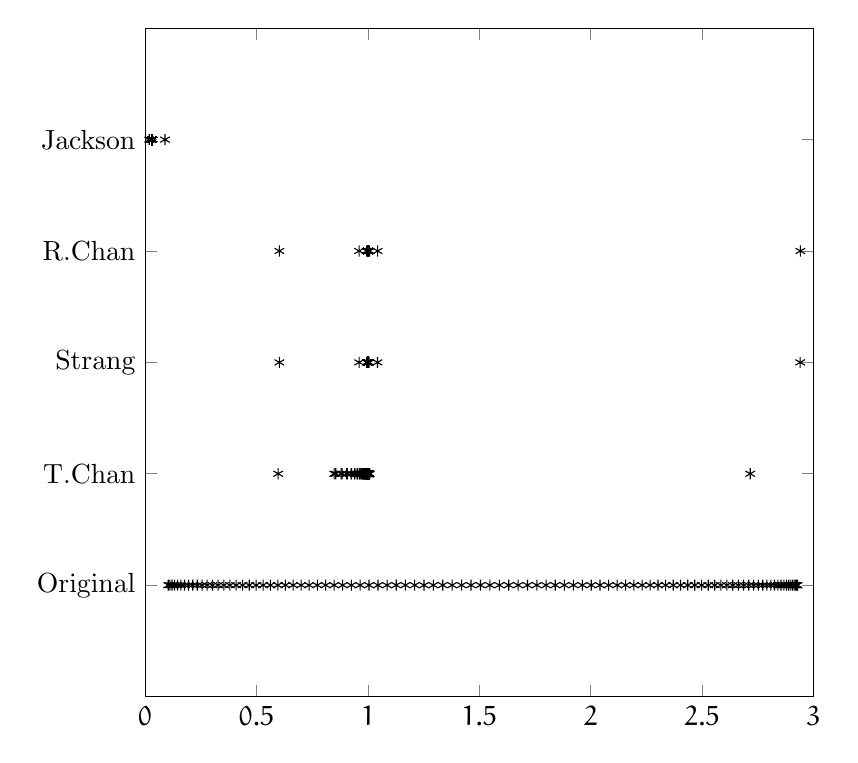
\begin{tikzpicture}

\begin{axis}[%
width=0.7\columnwidth,
height=0.7\columnwidth,
at={(0.758in,0.481in)},
scale only axis,
xmin=0,
xmax=3,
ymin=0,
ymax=6,
ytick={1,2,3,4,5},
yticklabels={{Original},{T.Chan},{Strang},{R.Chan},{Jackson}},
axis background/.style={fill=white}
]
\addplot [color=black, only marks, mark=asterisk, mark options={solid, black}, forget plot]
  table[row sep=crcr]{%
0.103814312414509	1\\
};
\addplot [color=black, only marks, mark=asterisk, mark options={solid, black}, forget plot]
  table[row sep=crcr]{%
0.111048653076966	1\\
};
\addplot [color=black, only marks, mark=asterisk, mark options={solid, black}, forget plot]
  table[row sep=crcr]{%
0.120625119900538	1\\
};
\addplot [color=black, only marks, mark=asterisk, mark options={solid, black}, forget plot]
  table[row sep=crcr]{%
0.132201788569615	1\\
};
\addplot [color=black, only marks, mark=asterisk, mark options={solid, black}, forget plot]
  table[row sep=crcr]{%
0.14550662951455	1\\
};
\addplot [color=black, only marks, mark=asterisk, mark options={solid, black}, forget plot]
  table[row sep=crcr]{%
0.160412007302882	1\\
};
\addplot [color=black, only marks, mark=asterisk, mark options={solid, black}, forget plot]
  table[row sep=crcr]{%
0.176791346715223	1\\
};
\addplot [color=black, only marks, mark=asterisk, mark options={solid, black}, forget plot]
  table[row sep=crcr]{%
0.194571264118084	1\\
};
\addplot [color=black, only marks, mark=asterisk, mark options={solid, black}, forget plot]
  table[row sep=crcr]{%
0.213673499334156	1\\
};
\addplot [color=black, only marks, mark=asterisk, mark options={solid, black}, forget plot]
  table[row sep=crcr]{%
0.234046580845932	1\\
};
\addplot [color=black, only marks, mark=asterisk, mark options={solid, black}, forget plot]
  table[row sep=crcr]{%
0.255633906381582	1\\
};
\addplot [color=black, only marks, mark=asterisk, mark options={solid, black}, forget plot]
  table[row sep=crcr]{%
0.278394603894795	1\\
};
\addplot [color=black, only marks, mark=asterisk, mark options={solid, black}, forget plot]
  table[row sep=crcr]{%
0.30228323352292	1\\
};
\addplot [color=black, only marks, mark=asterisk, mark options={solid, black}, forget plot]
  table[row sep=crcr]{%
0.327264468743062	1\\
};
\addplot [color=black, only marks, mark=asterisk, mark options={solid, black}, forget plot]
  table[row sep=crcr]{%
0.353299030702619	1\\
};
\addplot [color=black, only marks, mark=asterisk, mark options={solid, black}, forget plot]
  table[row sep=crcr]{%
0.380354537617579	1\\
};
\addplot [color=black, only marks, mark=asterisk, mark options={solid, black}, forget plot]
  table[row sep=crcr]{%
0.408395189593098	1\\
};
\addplot [color=black, only marks, mark=asterisk, mark options={solid, black}, forget plot]
  table[row sep=crcr]{%
0.437390085981798	1\\
};
\addplot [color=black, only marks, mark=asterisk, mark options={solid, black}, forget plot]
  table[row sep=crcr]{%
0.4673053512833	1\\
};
\addplot [color=black, only marks, mark=asterisk, mark options={solid, black}, forget plot]
  table[row sep=crcr]{%
0.498110694021965	1\\
};
\addplot [color=black, only marks, mark=asterisk, mark options={solid, black}, forget plot]
  table[row sep=crcr]{%
0.529773214740183	1\\
};
\addplot [color=black, only marks, mark=asterisk, mark options={solid, black}, forget plot]
  table[row sep=crcr]{%
0.562262694466092	1\\
};
\addplot [color=black, only marks, mark=asterisk, mark options={solid, black}, forget plot]
  table[row sep=crcr]{%
0.595546613277242	1\\
};
\addplot [color=black, only marks, mark=asterisk, mark options={solid, black}, forget plot]
  table[row sep=crcr]{%
0.629594491186748	1\\
};
\addplot [color=black, only marks, mark=asterisk, mark options={solid, black}, forget plot]
  table[row sep=crcr]{%
0.664373808276955	1\\
};
\addplot [color=black, only marks, mark=asterisk, mark options={solid, black}, forget plot]
  table[row sep=crcr]{%
0.699853619967369	1\\
};
\addplot [color=black, only marks, mark=asterisk, mark options={solid, black}, forget plot]
  table[row sep=crcr]{%
0.736001167437343	1\\
};
\addplot [color=black, only marks, mark=asterisk, mark options={solid, black}, forget plot]
  table[row sep=crcr]{%
0.772784924891706	1\\
};
\addplot [color=black, only marks, mark=asterisk, mark options={solid, black}, forget plot]
  table[row sep=crcr]{%
0.810171750713007	1\\
};
\addplot [color=black, only marks, mark=asterisk, mark options={solid, black}, forget plot]
  table[row sep=crcr]{%
0.848129481738572	1\\
};
\addplot [color=black, only marks, mark=asterisk, mark options={solid, black}, forget plot]
  table[row sep=crcr]{%
0.886624516173144	1\\
};
\addplot [color=black, only marks, mark=asterisk, mark options={solid, black}, forget plot]
  table[row sep=crcr]{%
0.925624040781602	1\\
};
\addplot [color=black, only marks, mark=asterisk, mark options={solid, black}, forget plot]
  table[row sep=crcr]{%
0.965093964201867	1\\
};
\addplot [color=black, only marks, mark=asterisk, mark options={solid, black}, forget plot]
  table[row sep=crcr]{%
1.00500084252033	1\\
};
\addplot [color=black, only marks, mark=asterisk, mark options={solid, black}, forget plot]
  table[row sep=crcr]{%
1.04531010094925	1\\
};
\addplot [color=black, only marks, mark=asterisk, mark options={solid, black}, forget plot]
  table[row sep=crcr]{%
1.08598770856128	1\\
};
\addplot [color=black, only marks, mark=asterisk, mark options={solid, black}, forget plot]
  table[row sep=crcr]{%
1.12699864015802	1\\
};
\addplot [color=black, only marks, mark=asterisk, mark options={solid, black}, forget plot]
  table[row sep=crcr]{%
1.16830834015994	1\\
};
\addplot [color=black, only marks, mark=asterisk, mark options={solid, black}, forget plot]
  table[row sep=crcr]{%
1.20988138665178	1\\
};
\addplot [color=black, only marks, mark=asterisk, mark options={solid, black}, forget plot]
  table[row sep=crcr]{%
1.25168277636821	1\\
};
\addplot [color=black, only marks, mark=asterisk, mark options={solid, black}, forget plot]
  table[row sep=crcr]{%
1.29367676048781	1\\
};
\addplot [color=black, only marks, mark=asterisk, mark options={solid, black}, forget plot]
  table[row sep=crcr]{%
1.33582797653632	1\\
};
\addplot [color=black, only marks, mark=asterisk, mark options={solid, black}, forget plot]
  table[row sep=crcr]{%
1.37810043126042	1\\
};
\addplot [color=black, only marks, mark=asterisk, mark options={solid, black}, forget plot]
  table[row sep=crcr]{%
1.42045850055561	1\\
};
\addplot [color=black, only marks, mark=asterisk, mark options={solid, black}, forget plot]
  table[row sep=crcr]{%
1.46286603918887	1\\
};
\addplot [color=black, only marks, mark=asterisk, mark options={solid, black}, forget plot]
  table[row sep=crcr]{%
1.50528726617781	1\\
};
\addplot [color=black, only marks, mark=asterisk, mark options={solid, black}, forget plot]
  table[row sep=crcr]{%
1.54768598459614	1\\
};
\addplot [color=black, only marks, mark=asterisk, mark options={solid, black}, forget plot]
  table[row sep=crcr]{%
1.59002636692381	1\\
};
\addplot [color=black, only marks, mark=asterisk, mark options={solid, black}, forget plot]
  table[row sep=crcr]{%
1.63227227090723	1\\
};
\addplot [color=black, only marks, mark=asterisk, mark options={solid, black}, forget plot]
  table[row sep=crcr]{%
1.67438793707972	1\\
};
\addplot [color=black, only marks, mark=asterisk, mark options={solid, black}, forget plot]
  table[row sep=crcr]{%
1.71633738883529	1\\
};
\addplot [color=black, only marks, mark=asterisk, mark options={solid, black}, forget plot]
  table[row sep=crcr]{%
1.75808505244864	1\\
};
\addplot [color=black, only marks, mark=asterisk, mark options={solid, black}, forget plot]
  table[row sep=crcr]{%
1.79959523128545	1\\
};
\addplot [color=black, only marks, mark=asterisk, mark options={solid, black}, forget plot]
  table[row sep=crcr]{%
1.84083265713077	1\\
};
\addplot [color=black, only marks, mark=asterisk, mark options={solid, black}, forget plot]
  table[row sep=crcr]{%
1.88176202989476	1\\
};
\addplot [color=black, only marks, mark=asterisk, mark options={solid, black}, forget plot]
  table[row sep=crcr]{%
1.92234850781242	1\\
};
\addplot [color=black, only marks, mark=asterisk, mark options={solid, black}, forget plot]
  table[row sep=crcr]{%
1.96255730518187	1\\
};
\addplot [color=black, only marks, mark=asterisk, mark options={solid, black}, forget plot]
  table[row sep=crcr]{%
2.00235412797029	1\\
};
\addplot [color=black, only marks, mark=asterisk, mark options={solid, black}, forget plot]
  table[row sep=crcr]{%
2.04170482309627	1\\
};
\addplot [color=black, only marks, mark=asterisk, mark options={solid, black}, forget plot]
  table[row sep=crcr]{%
2.08057576512242	1\\
};
\addplot [color=black, only marks, mark=asterisk, mark options={solid, black}, forget plot]
  table[row sep=crcr]{%
2.11893355140444	1\\
};
\addplot [color=black, only marks, mark=asterisk, mark options={solid, black}, forget plot]
  table[row sep=crcr]{%
2.15674534483739	1\\
};
\addplot [color=black, only marks, mark=asterisk, mark options={solid, black}, forget plot]
  table[row sep=crcr]{%
2.19397860987363	1\\
};
\addplot [color=black, only marks, mark=asterisk, mark options={solid, black}, forget plot]
  table[row sep=crcr]{%
2.23060141569027	1\\
};
\addplot [color=black, only marks, mark=asterisk, mark options={solid, black}, forget plot]
  table[row sep=crcr]{%
2.26658220865087	1\\
};
\addplot [color=black, only marks, mark=asterisk, mark options={solid, black}, forget plot]
  table[row sep=crcr]{%
2.30189007975573	1\\
};
\addplot [color=black, only marks, mark=asterisk, mark options={solid, black}, forget plot]
  table[row sep=crcr]{%
2.33649456960757	1\\
};
\addplot [color=black, only marks, mark=asterisk, mark options={solid, black}, forget plot]
  table[row sep=crcr]{%
2.3703659035777	1\\
};
\addplot [color=black, only marks, mark=asterisk, mark options={solid, black}, forget plot]
  table[row sep=crcr]{%
2.40347482574885	1\\
};
\addplot [color=black, only marks, mark=asterisk, mark options={solid, black}, forget plot]
  table[row sep=crcr]{%
2.43579280486625	1\\
};
\addplot [color=black, only marks, mark=asterisk, mark options={solid, black}, forget plot]
  table[row sep=crcr]{%
2.46729189408367	1\\
};
\addplot [color=black, only marks, mark=asterisk, mark options={solid, black}, forget plot]
  table[row sep=crcr]{%
2.49794491045798	1\\
};
\addplot [color=black, only marks, mark=asterisk, mark options={solid, black}, forget plot]
  table[row sep=crcr]{%
2.52772531762761	1\\
};
\addplot [color=black, only marks, mark=asterisk, mark options={solid, black}, forget plot]
  table[row sep=crcr]{%
2.55660738134397	1\\
};
\addplot [color=black, only marks, mark=asterisk, mark options={solid, black}, forget plot]
  table[row sep=crcr]{%
2.58456607247223	1\\
};
\addplot [color=black, only marks, mark=asterisk, mark options={solid, black}, forget plot]
  table[row sep=crcr]{%
2.61157720082655	1\\
};
\addplot [color=black, only marks, mark=asterisk, mark options={solid, black}, forget plot]
  table[row sep=crcr]{%
2.637617336108	1\\
};
\addplot [color=black, only marks, mark=asterisk, mark options={solid, black}, forget plot]
  table[row sep=crcr]{%
2.66266392211675	1\\
};
\addplot [color=black, only marks, mark=asterisk, mark options={solid, black}, forget plot]
  table[row sep=crcr]{%
2.6866952134367	1\\
};
\addplot [color=black, only marks, mark=asterisk, mark options={solid, black}, forget plot]
  table[row sep=crcr]{%
2.70969037193205	1\\
};
\addplot [color=black, only marks, mark=asterisk, mark options={solid, black}, forget plot]
  table[row sep=crcr]{%
2.73162941715664	1\\
};
\addplot [color=black, only marks, mark=asterisk, mark options={solid, black}, forget plot]
  table[row sep=crcr]{%
2.75249330690137	1\\
};
\addplot [color=black, only marks, mark=asterisk, mark options={solid, black}, forget plot]
  table[row sep=crcr]{%
2.77226389945179	1\\
};
\addplot [color=black, only marks, mark=asterisk, mark options={solid, black}, forget plot]
  table[row sep=crcr]{%
2.79092401983315	1\\
};
\addplot [color=black, only marks, mark=asterisk, mark options={solid, black}, forget plot]
  table[row sep=crcr]{%
2.80845743216586	1\\
};
\addplot [color=black, only marks, mark=asterisk, mark options={solid, black}, forget plot]
  table[row sep=crcr]{%
2.82484889315364	1\\
};
\addplot [color=black, only marks, mark=asterisk, mark options={solid, black}, forget plot]
  table[row sep=crcr]{%
2.84008413289529	1\\
};
\addplot [color=black, only marks, mark=asterisk, mark options={solid, black}, forget plot]
  table[row sep=crcr]{%
2.85414989707688	1\\
};
\addplot [color=black, only marks, mark=asterisk, mark options={solid, black}, forget plot]
  table[row sep=crcr]{%
2.86703393469155	1\\
};
\addplot [color=black, only marks, mark=asterisk, mark options={solid, black}, forget plot]
  table[row sep=crcr]{%
2.87872503032677	1\\
};
\addplot [color=black, only marks, mark=asterisk, mark options={solid, black}, forget plot]
  table[row sep=crcr]{%
2.88921299732346	1\\
};
\addplot [color=black, only marks, mark=asterisk, mark options={solid, black}, forget plot]
  table[row sep=crcr]{%
2.89848870149311	1\\
};
\addplot [color=black, only marks, mark=asterisk, mark options={solid, black}, forget plot]
  table[row sep=crcr]{%
2.90654405831427	1\\
};
\addplot [color=black, only marks, mark=asterisk, mark options={solid, black}, forget plot]
  table[row sep=crcr]{%
2.91337204937011	1\\
};
\addplot [color=black, only marks, mark=asterisk, mark options={solid, black}, forget plot]
  table[row sep=crcr]{%
2.91896672223595	1\\
};
\addplot [color=black, only marks, mark=asterisk, mark options={solid, black}, forget plot]
  table[row sep=crcr]{%
2.92332320089478	1\\
};
\addplot [color=black, only marks, mark=asterisk, mark options={solid, black}, forget plot]
  table[row sep=crcr]{%
2.92643768701429	1\\
};
\addplot [color=black, only marks, mark=asterisk, mark options={solid, black}, forget plot]
  table[row sep=crcr]{%
2.92830746557542	1\\
};
\addplot [color=black, only marks, mark=asterisk, mark options={solid, black}, forget plot]
  table[row sep=crcr]{%
2.71615944481265	2\\
};
\addplot [color=black, only marks, mark=asterisk, mark options={solid, black}, forget plot]
  table[row sep=crcr]{%
0.597174881084976	2\\
};
\addplot [color=black, only marks, mark=asterisk, mark options={solid, black}, forget plot]
  table[row sep=crcr]{%
0.848381736567241	2\\
};
\addplot [color=black, only marks, mark=asterisk, mark options={solid, black}, forget plot]
  table[row sep=crcr]{%
0.855685638804306	2\\
};
\addplot [color=black, only marks, mark=asterisk, mark options={solid, black}, forget plot]
  table[row sep=crcr]{%
0.879469277381942	2\\
};
\addplot [color=black, only marks, mark=asterisk, mark options={solid, black}, forget plot]
  table[row sep=crcr]{%
0.883456347637111	2\\
};
\addplot [color=black, only marks, mark=asterisk, mark options={solid, black}, forget plot]
  table[row sep=crcr]{%
0.904659831034027	2\\
};
\addplot [color=black, only marks, mark=asterisk, mark options={solid, black}, forget plot]
  table[row sep=crcr]{%
0.907274795507846	2\\
};
\addplot [color=black, only marks, mark=asterisk, mark options={solid, black}, forget plot]
  table[row sep=crcr]{%
0.924731462066746	2\\
};
\addplot [color=black, only marks, mark=asterisk, mark options={solid, black}, forget plot]
  table[row sep=crcr]{%
0.926307157935132	2\\
};
\addplot [color=black, only marks, mark=asterisk, mark options={solid, black}, forget plot]
  table[row sep=crcr]{%
0.940287757236584	2\\
};
\addplot [color=black, only marks, mark=asterisk, mark options={solid, black}, forget plot]
  table[row sep=crcr]{%
0.94114765796302	2\\
};
\addplot [color=black, only marks, mark=asterisk, mark options={solid, black}, forget plot]
  table[row sep=crcr]{%
0.952664818668304	2\\
};
\addplot [color=black, only marks, mark=asterisk, mark options={solid, black}, forget plot]
  table[row sep=crcr]{%
0.95226339345437	2\\
};
\addplot [color=black, only marks, mark=asterisk, mark options={solid, black}, forget plot]
  table[row sep=crcr]{%
0.961645804555014	2\\
};
\addplot [color=black, only marks, mark=asterisk, mark options={solid, black}, forget plot]
  table[row sep=crcr]{%
0.961525316414568	2\\
};
\addplot [color=black, only marks, mark=asterisk, mark options={solid, black}, forget plot]
  table[row sep=crcr]{%
0.968714100329372	2\\
};
\addplot [color=black, only marks, mark=asterisk, mark options={solid, black}, forget plot]
  table[row sep=crcr]{%
0.968760082112865	2\\
};
\addplot [color=black, only marks, mark=asterisk, mark options={solid, black}, forget plot]
  table[row sep=crcr]{%
0.9743389516307	2\\
};
\addplot [color=black, only marks, mark=asterisk, mark options={solid, black}, forget plot]
  table[row sep=crcr]{%
0.974479948431481	2\\
};
\addplot [color=black, only marks, mark=asterisk, mark options={solid, black}, forget plot]
  table[row sep=crcr]{%
0.978867073748429	2\\
};
\addplot [color=black, only marks, mark=asterisk, mark options={solid, black}, forget plot]
  table[row sep=crcr]{%
0.979059201926603	2\\
};
\addplot [color=black, only marks, mark=asterisk, mark options={solid, black}, forget plot]
  table[row sep=crcr]{%
0.98255379515527	2\\
};
\addplot [color=black, only marks, mark=asterisk, mark options={solid, black}, forget plot]
  table[row sep=crcr]{%
0.982770382081343	2\\
};
\addplot [color=black, only marks, mark=asterisk, mark options={solid, black}, forget plot]
  table[row sep=crcr]{%
0.985587927593152	2\\
};
\addplot [color=black, only marks, mark=asterisk, mark options={solid, black}, forget plot]
  table[row sep=crcr]{%
0.98581293431552	2\\
};
\addplot [color=black, only marks, mark=asterisk, mark options={solid, black}, forget plot]
  table[row sep=crcr]{%
0.988110203722665	2\\
};
\addplot [color=black, only marks, mark=asterisk, mark options={solid, black}, forget plot]
  table[row sep=crcr]{%
0.988334141725408	2\\
};
\addplot [color=black, only marks, mark=asterisk, mark options={solid, black}, forget plot]
  table[row sep=crcr]{%
0.990226544064756	2\\
};
\addplot [color=black, only marks, mark=asterisk, mark options={solid, black}, forget plot]
  table[row sep=crcr]{%
0.990443958357679	2\\
};
\addplot [color=black, only marks, mark=asterisk, mark options={solid, black}, forget plot]
  table[row sep=crcr]{%
0.992017505539622	2\\
};
\addplot [color=black, only marks, mark=asterisk, mark options={solid, black}, forget plot]
  table[row sep=crcr]{%
0.992225422862911	2\\
};
\addplot [color=black, only marks, mark=asterisk, mark options={solid, black}, forget plot]
  table[row sep=crcr]{%
0.993545006832322	2\\
};
\addplot [color=black, only marks, mark=asterisk, mark options={solid, black}, forget plot]
  table[row sep=crcr]{%
0.993741975502515	2\\
};
\addplot [color=black, only marks, mark=asterisk, mark options={solid, black}, forget plot]
  table[row sep=crcr]{%
0.994857137431647	2\\
};
\addplot [color=black, only marks, mark=asterisk, mark options={solid, black}, forget plot]
  table[row sep=crcr]{%
0.995042630557042	2\\
};
\addplot [color=black, only marks, mark=asterisk, mark options={solid, black}, forget plot]
  table[row sep=crcr]{%
1.00801647480245	2\\
};
\addplot [color=black, only marks, mark=asterisk, mark options={solid, black}, forget plot]
  table[row sep=crcr]{%
0.995991621724546	2\\
};
\addplot [color=black, only marks, mark=asterisk, mark options={solid, black}, forget plot]
  table[row sep=crcr]{%
0.996165664770168	2\\
};
\addplot [color=black, only marks, mark=asterisk, mark options={solid, black}, forget plot]
  table[row sep=crcr]{%
0.996978336288691	2\\
};
\addplot [color=black, only marks, mark=asterisk, mark options={solid, black}, forget plot]
  table[row sep=crcr]{%
0.997141274084967	2\\
};
\addplot [color=black, only marks, mark=asterisk, mark options={solid, black}, forget plot]
  table[row sep=crcr]{%
0.997841156529152	2\\
};
\addplot [color=black, only marks, mark=asterisk, mark options={solid, black}, forget plot]
  table[row sep=crcr]{%
0.99799350754821	2\\
};
\addplot [color=black, only marks, mark=asterisk, mark options={solid, black}, forget plot]
  table[row sep=crcr]{%
0.998599324492917	2\\
};
\addplot [color=black, only marks, mark=asterisk, mark options={solid, black}, forget plot]
  table[row sep=crcr]{%
0.998741690081634	2\\
};
\addplot [color=black, only marks, mark=asterisk, mark options={solid, black}, forget plot]
  table[row sep=crcr]{%
0.999268471801508	2\\
};
\addplot [color=black, only marks, mark=asterisk, mark options={solid, black}, forget plot]
  table[row sep=crcr]{%
0.999401480197064	2\\
};
\addplot [color=black, only marks, mark=asterisk, mark options={solid, black}, forget plot]
  table[row sep=crcr]{%
0.999861391880214	2\\
};
\addplot [color=black, only marks, mark=asterisk, mark options={solid, black}, forget plot]
  table[row sep=crcr]{%
0.999985664310335	2\\
};
\addplot [color=black, only marks, mark=asterisk, mark options={solid, black}, forget plot]
  table[row sep=crcr]{%
1.00038862824459	2\\
};
\addplot [color=black, only marks, mark=asterisk, mark options={solid, black}, forget plot]
  table[row sep=crcr]{%
1.00050475906039	2\\
};
\addplot [color=black, only marks, mark=asterisk, mark options={solid, black}, forget plot]
  table[row sep=crcr]{%
1.00085892658076	2\\
};
\addplot [color=black, only marks, mark=asterisk, mark options={solid, black}, forget plot]
  table[row sep=crcr]{%
1.00096747228304	2\\
};
\addplot [color=black, only marks, mark=asterisk, mark options={solid, black}, forget plot]
  table[row sep=crcr]{%
1.00127958505752	2\\
};
\addplot [color=black, only marks, mark=asterisk, mark options={solid, black}, forget plot]
  table[row sep=crcr]{%
1.00138105891913	2\\
};
\addplot [color=black, only marks, mark=asterisk, mark options={solid, black}, forget plot]
  table[row sep=crcr]{%
1.00165672793578	2\\
};
\addplot [color=black, only marks, mark=asterisk, mark options={solid, black}, forget plot]
  table[row sep=crcr]{%
1.00175159809658	2\\
};
\addplot [color=black, only marks, mark=asterisk, mark options={solid, black}, forget plot]
  table[row sep=crcr]{%
1.0019955208795	2\\
};
\addplot [color=black, only marks, mark=asterisk, mark options={solid, black}, forget plot]
  table[row sep=crcr]{%
1.00208421054379	2\\
};
\addplot [color=black, only marks, mark=asterisk, mark options={solid, black}, forget plot]
  table[row sep=crcr]{%
1.00230034159664	2\\
};
\addplot [color=black, only marks, mark=asterisk, mark options={solid, black}, forget plot]
  table[row sep=crcr]{%
1.00238323044944	2\\
};
\addplot [color=black, only marks, mark=asterisk, mark options={solid, black}, forget plot]
  table[row sep=crcr]{%
1.00257491598597	2\\
};
\addplot [color=black, only marks, mark=asterisk, mark options={solid, black}, forget plot]
  table[row sep=crcr]{%
1.0026523422602	2\\
};
\addplot [color=black, only marks, mark=asterisk, mark options={solid, black}, forget plot]
  table[row sep=crcr]{%
1.00282242744802	2\\
};
\addplot [color=black, only marks, mark=asterisk, mark options={solid, black}, forget plot]
  table[row sep=crcr]{%
1.00289469027992	2\\
};
\addplot [color=black, only marks, mark=asterisk, mark options={solid, black}, forget plot]
  table[row sep=crcr]{%
1.003045605168	2\\
};
\addplot [color=black, only marks, mark=asterisk, mark options={solid, black}, forget plot]
  table[row sep=crcr]{%
1.00311296701209	2\\
};
\addplot [color=black, only marks, mark=asterisk, mark options={solid, black}, forget plot]
  table[row sep=crcr]{%
1.00324679580713	2\\
};
\addplot [color=black, only marks, mark=asterisk, mark options={solid, black}, forget plot]
  table[row sep=crcr]{%
1.00330948476911	2\\
};
\addplot [color=black, only marks, mark=asterisk, mark options={solid, black}, forget plot]
  table[row sep=crcr]{%
1.00342802201503	2\\
};
\addplot [color=black, only marks, mark=asterisk, mark options={solid, black}, forget plot]
  table[row sep=crcr]{%
1.00348623401731	2\\
};
\addplot [color=black, only marks, mark=asterisk, mark options={solid, black}, forget plot]
  table[row sep=crcr]{%
1.00359103040517	2\\
};
\addplot [color=black, only marks, mark=asterisk, mark options={solid, black}, forget plot]
  table[row sep=crcr]{%
1.00364493113611	2\\
};
\addplot [color=black, only marks, mark=asterisk, mark options={solid, black}, forget plot]
  table[row sep=crcr]{%
1.00373733105196	2\\
};
\addplot [color=black, only marks, mark=asterisk, mark options={solid, black}, forget plot]
  table[row sep=crcr]{%
1.00378705767237	2\\
};
\addplot [color=black, only marks, mark=asterisk, mark options={solid, black}, forget plot]
  table[row sep=crcr]{%
1.00386823012217	2\\
};
\addplot [color=black, only marks, mark=asterisk, mark options={solid, black}, forget plot]
  table[row sep=crcr]{%
1.00391389271664	2\\
};
\addplot [color=black, only marks, mark=asterisk, mark options={solid, black}, forget plot]
  table[row sep=crcr]{%
1.00398485691112	2\\
};
\addplot [color=black, only marks, mark=asterisk, mark options={solid, black}, forget plot]
  table[row sep=crcr]{%
1.00402653967938	2\\
};
\addplot [color=black, only marks, mark=asterisk, mark options={solid, black}, forget plot]
  table[row sep=crcr]{%
1.00408818628895	2\\
};
\addplot [color=black, only marks, mark=asterisk, mark options={solid, black}, forget plot]
  table[row sep=crcr]{%
1.00412594847665	2\\
};
\addplot [color=black, only marks, mark=asterisk, mark options={solid, black}, forget plot]
  table[row sep=crcr]{%
1.00417905735598	2\\
};
\addplot [color=black, only marks, mark=asterisk, mark options={solid, black}, forget plot]
  table[row sep=crcr]{%
1.00421293392508	2\\
};
\addplot [color=black, only marks, mark=asterisk, mark options={solid, black}, forget plot]
  table[row sep=crcr]{%
1.00425818894413	2\\
};
\addplot [color=black, only marks, mark=asterisk, mark options={solid, black}, forget plot]
  table[row sep=crcr]{%
1.0042881909824	2\\
};
\addplot [color=black, only marks, mark=asterisk, mark options={solid, black}, forget plot]
  table[row sep=crcr]{%
1.00432619247325	2\\
};
\addplot [color=black, only marks, mark=asterisk, mark options={solid, black}, forget plot]
  table[row sep=crcr]{%
1.00435230734041	2\\
};
\addplot [color=black, only marks, mark=asterisk, mark options={solid, black}, forget plot]
  table[row sep=crcr]{%
1.0043835825693	2\\
};
\addplot [color=black, only marks, mark=asterisk, mark options={solid, black}, forget plot]
  table[row sep=crcr]{%
1.004405773774	2\\
};
\addplot [color=black, only marks, mark=asterisk, mark options={solid, black}, forget plot]
  table[row sep=crcr]{%
1.00443078576926	2\\
};
\addplot [color=black, only marks, mark=asterisk, mark options={solid, black}, forget plot]
  table[row sep=crcr]{%
1.0044489925672	2\\
};
\addplot [color=black, only marks, mark=asterisk, mark options={solid, black}, forget plot]
  table[row sep=crcr]{%
1.00446814757115	2\\
};
\addplot [color=black, only marks, mark=asterisk, mark options={solid, black}, forget plot]
  table[row sep=crcr]{%
1.00448228426969	2\\
};
\addplot [color=black, only marks, mark=asterisk, mark options={solid, black}, forget plot]
  table[row sep=crcr]{%
1.00452353262051	2\\
};
\addplot [color=black, only marks, mark=asterisk, mark options={solid, black}, forget plot]
  table[row sep=crcr]{%
1.00451999031968	2\\
};
\addplot [color=black, only marks, mark=asterisk, mark options={solid, black}, forget plot]
  table[row sep=crcr]{%
1.00451435607638	2\\
};
\addplot [color=black, only marks, mark=asterisk, mark options={solid, black}, forget plot]
  table[row sep=crcr]{%
1.00449593803266	2\\
};
\addplot [color=black, only marks, mark=asterisk, mark options={solid, black}, forget plot]
  table[row sep=crcr]{%
1.00450589298186	2\\
};
\addplot [color=black, only marks, mark=asterisk, mark options={solid, black}, forget plot]
  table[row sep=crcr]{%
2.94026487859607	3\\
};
\addplot [color=black, only marks, mark=asterisk, mark options={solid, black}, forget plot]
  table[row sep=crcr]{%
0.602469818073853	3\\
};
\addplot [color=black, only marks, mark=asterisk, mark options={solid, black}, forget plot]
  table[row sep=crcr]{%
1.04288712791385	3\\
};
\addplot [color=black, only marks, mark=asterisk, mark options={solid, black}, forget plot]
  table[row sep=crcr]{%
0.96053229755332	3\\
};
\addplot [color=black, only marks, mark=asterisk, mark options={solid, black}, forget plot]
  table[row sep=crcr]{%
1.00565979732679	3\\
};
\addplot [color=black, only marks, mark=asterisk, mark options={solid, black}, forget plot]
  table[row sep=crcr]{%
0.994410679587501	3\\
};
\addplot [color=black, only marks, mark=asterisk, mark options={solid, black}, forget plot]
  table[row sep=crcr]{%
0.999350223802997	3\\
};
\addplot [color=black, only marks, mark=asterisk, mark options={solid, black}, forget plot]
  table[row sep=crcr]{%
1.00065073351505	3\\
};
\addplot [color=black, only marks, mark=asterisk, mark options={solid, black}, forget plot]
  table[row sep=crcr]{%
0.999657960245326	3\\
};
\addplot [color=black, only marks, mark=asterisk, mark options={solid, black}, forget plot]
  table[row sep=crcr]{%
1.00034068881962	3\\
};
\addplot [color=black, only marks, mark=asterisk, mark options={solid, black}, forget plot]
  table[row sep=crcr]{%
0.999857841717831	3\\
};
\addplot [color=black, only marks, mark=asterisk, mark options={solid, black}, forget plot]
  table[row sep=crcr]{%
1.0001422653916	3\\
};
\addplot [color=black, only marks, mark=asterisk, mark options={solid, black}, forget plot]
  table[row sep=crcr]{%
0.999914335811072	3\\
};
\addplot [color=black, only marks, mark=asterisk, mark options={solid, black}, forget plot]
  table[row sep=crcr]{%
1.0000854874904	3\\
};
\addplot [color=black, only marks, mark=asterisk, mark options={solid, black}, forget plot]
  table[row sep=crcr]{%
0.999939149414482	3\\
};
\addplot [color=black, only marks, mark=asterisk, mark options={solid, black}, forget plot]
  table[row sep=crcr]{%
1.0000608725204	3\\
};
\addplot [color=black, only marks, mark=asterisk, mark options={solid, black}, forget plot]
  table[row sep=crcr]{%
0.999955894145746	3\\
};
\addplot [color=black, only marks, mark=asterisk, mark options={solid, black}, forget plot]
  table[row sep=crcr]{%
1.0000440439175	3\\
};
\addplot [color=black, only marks, mark=asterisk, mark options={solid, black}, forget plot]
  table[row sep=crcr]{%
0.999964177905466	3\\
};
\addplot [color=black, only marks, mark=asterisk, mark options={solid, black}, forget plot]
  table[row sep=crcr]{%
1.0000358291349	3\\
};
\addplot [color=black, only marks, mark=asterisk, mark options={solid, black}, forget plot]
  table[row sep=crcr]{%
0.999971396854776	3\\
};
\addplot [color=black, only marks, mark=asterisk, mark options={solid, black}, forget plot]
  table[row sep=crcr]{%
1.00002857277744	3\\
};
\addplot [color=black, only marks, mark=asterisk, mark options={solid, black}, forget plot]
  table[row sep=crcr]{%
0.999975458684443	3\\
};
\addplot [color=black, only marks, mark=asterisk, mark options={solid, black}, forget plot]
  table[row sep=crcr]{%
1.00002454430032	3\\
};
\addplot [color=black, only marks, mark=asterisk, mark options={solid, black}, forget plot]
  table[row sep=crcr]{%
0.999979265121479	3\\
};
\addplot [color=black, only marks, mark=asterisk, mark options={solid, black}, forget plot]
  table[row sep=crcr]{%
1.00002071733978	3\\
};
\addplot [color=black, only marks, mark=asterisk, mark options={solid, black}, forget plot]
  table[row sep=crcr]{%
0.99998168012418	3\\
};
\addplot [color=black, only marks, mark=asterisk, mark options={solid, black}, forget plot]
  table[row sep=crcr]{%
1.00001832137989	3\\
};
\addplot [color=black, only marks, mark=asterisk, mark options={solid, black}, forget plot]
  table[row sep=crcr]{%
0.999983943776496	3\\
};
\addplot [color=black, only marks, mark=asterisk, mark options={solid, black}, forget plot]
  table[row sep=crcr]{%
1.00001604511565	3\\
};
\addplot [color=black, only marks, mark=asterisk, mark options={solid, black}, forget plot]
  table[row sep=crcr]{%
0.999985545311572	3\\
};
\addplot [color=black, only marks, mark=asterisk, mark options={solid, black}, forget plot]
  table[row sep=crcr]{%
1.00001445553891	3\\
};
\addplot [color=black, only marks, mark=asterisk, mark options={solid, black}, forget plot]
  table[row sep=crcr]{%
0.999987002613152	3\\
};
\addplot [color=black, only marks, mark=asterisk, mark options={solid, black}, forget plot]
  table[row sep=crcr]{%
1.00001298993758	3\\
};
\addplot [color=black, only marks, mark=asterisk, mark options={solid, black}, forget plot]
  table[row sep=crcr]{%
0.999988138512285	3\\
};
\addplot [color=black, only marks, mark=asterisk, mark options={solid, black}, forget plot]
  table[row sep=crcr]{%
1.00001186201025	3\\
};
\addplot [color=black, only marks, mark=asterisk, mark options={solid, black}, forget plot]
  table[row sep=crcr]{%
0.999989131221243	3\\
};
\addplot [color=black, only marks, mark=asterisk, mark options={solid, black}, forget plot]
  table[row sep=crcr]{%
1.00001086358983	3\\
};
\addplot [color=black, only marks, mark=asterisk, mark options={solid, black}, forget plot]
  table[row sep=crcr]{%
0.99998997291653	3\\
};
\addplot [color=black, only marks, mark=asterisk, mark options={solid, black}, forget plot]
  table[row sep=crcr]{%
1.00001002742577	3\\
};
\addplot [color=black, only marks, mark=asterisk, mark options={solid, black}, forget plot]
  table[row sep=crcr]{%
0.999990678514817	3\\
};
\addplot [color=black, only marks, mark=asterisk, mark options={solid, black}, forget plot]
  table[row sep=crcr]{%
1.00000931777558	3\\
};
\addplot [color=black, only marks, mark=asterisk, mark options={solid, black}, forget plot]
  table[row sep=crcr]{%
0.999991320899555	3\\
};
\addplot [color=black, only marks, mark=asterisk, mark options={solid, black}, forget plot]
  table[row sep=crcr]{%
1.00000867933676	3\\
};
\addplot [color=black, only marks, mark=asterisk, mark options={solid, black}, forget plot]
  table[row sep=crcr]{%
0.999991839325441	3\\
};
\addplot [color=black, only marks, mark=asterisk, mark options={solid, black}, forget plot]
  table[row sep=crcr]{%
1.00000815797586	3\\
};
\addplot [color=black, only marks, mark=asterisk, mark options={solid, black}, forget plot]
  table[row sep=crcr]{%
0.999992339564162	3\\
};
\addplot [color=black, only marks, mark=asterisk, mark options={solid, black}, forget plot]
  table[row sep=crcr]{%
1.0000076606065	3\\
};
\addplot [color=black, only marks, mark=asterisk, mark options={solid, black}, forget plot]
  table[row sep=crcr]{%
0.999992730600736	3\\
};
\addplot [color=black, only marks, mark=asterisk, mark options={solid, black}, forget plot]
  table[row sep=crcr]{%
1.00000726741563	3\\
};
\addplot [color=black, only marks, mark=asterisk, mark options={solid, black}, forget plot]
  table[row sep=crcr]{%
0.999993125383914	3\\
};
\addplot [color=black, only marks, mark=asterisk, mark options={solid, black}, forget plot]
  table[row sep=crcr]{%
1.00000687474434	3\\
};
\addplot [color=black, only marks, mark=asterisk, mark options={solid, black}, forget plot]
  table[row sep=crcr]{%
1.00000236011147	3\\
};
\addplot [color=black, only marks, mark=asterisk, mark options={solid, black}, forget plot]
  table[row sep=crcr]{%
0.999997611388056	3\\
};
\addplot [color=black, only marks, mark=asterisk, mark options={solid, black}, forget plot]
  table[row sep=crcr]{%
0.999993426493106	3\\
};
\addplot [color=black, only marks, mark=asterisk, mark options={solid, black}, forget plot]
  table[row sep=crcr]{%
1.00000657204401	3\\
};
\addplot [color=black, only marks, mark=asterisk, mark options={solid, black}, forget plot]
  table[row sep=crcr]{%
1.00000625956169	3\\
};
\addplot [color=black, only marks, mark=asterisk, mark options={solid, black}, forget plot]
  table[row sep=crcr]{%
0.999993740538256	3\\
};
\addplot [color=black, only marks, mark=asterisk, mark options={solid, black}, forget plot]
  table[row sep=crcr]{%
0.999999905151445	3\\
};
\addplot [color=black, only marks, mark=asterisk, mark options={solid, black}, forget plot]
  table[row sep=crcr]{%
1.0000000924628	3\\
};
\addplot [color=black, only marks, mark=asterisk, mark options={solid, black}, forget plot]
  table[row sep=crcr]{%
0.999993976055137	3\\
};
\addplot [color=black, only marks, mark=asterisk, mark options={solid, black}, forget plot]
  table[row sep=crcr]{%
0.999994226649237	3\\
};
\addplot [color=black, only marks, mark=asterisk, mark options={solid, black}, forget plot]
  table[row sep=crcr]{%
0.999994412820415	3\\
};
\addplot [color=black, only marks, mark=asterisk, mark options={solid, black}, forget plot]
  table[row sep=crcr]{%
0.99999461241143	3\\
};
\addplot [color=black, only marks, mark=asterisk, mark options={solid, black}, forget plot]
  table[row sep=crcr]{%
0.99999476029386	3\\
};
\addplot [color=black, only marks, mark=asterisk, mark options={solid, black}, forget plot]
  table[row sep=crcr]{%
0.999994918049989	3\\
};
\addplot [color=black, only marks, mark=asterisk, mark options={solid, black}, forget plot]
  table[row sep=crcr]{%
0.999995035245505	3\\
};
\addplot [color=black, only marks, mark=asterisk, mark options={solid, black}, forget plot]
  table[row sep=crcr]{%
0.999995158034182	3\\
};
\addplot [color=black, only marks, mark=asterisk, mark options={solid, black}, forget plot]
  table[row sep=crcr]{%
0.999995249760653	3\\
};
\addplot [color=black, only marks, mark=asterisk, mark options={solid, black}, forget plot]
  table[row sep=crcr]{%
0.999995342783158	3\\
};
\addplot [color=black, only marks, mark=asterisk, mark options={solid, black}, forget plot]
  table[row sep=crcr]{%
0.999995629560323	3\\
};
\addplot [color=black, only marks, mark=asterisk, mark options={solid, black}, forget plot]
  table[row sep=crcr]{%
0.999995643159203	3\\
};
\addplot [color=black, only marks, mark=asterisk, mark options={solid, black}, forget plot]
  table[row sep=crcr]{%
0.999995574204475	3\\
};
\addplot [color=black, only marks, mark=asterisk, mark options={solid, black}, forget plot]
  table[row sep=crcr]{%
0.999995605804204	3\\
};
\addplot [color=black, only marks, mark=asterisk, mark options={solid, black}, forget plot]
  table[row sep=crcr]{%
0.999995479763577	3\\
};
\addplot [color=black, only marks, mark=asterisk, mark options={solid, black}, forget plot]
  table[row sep=crcr]{%
0.99999552981915	3\\
};
\addplot [color=black, only marks, mark=asterisk, mark options={solid, black}, forget plot]
  table[row sep=crcr]{%
0.999995412552607	3\\
};
\addplot [color=black, only marks, mark=asterisk, mark options={solid, black}, forget plot]
  table[row sep=crcr]{%
1.00000602287081	3\\
};
\addplot [color=black, only marks, mark=asterisk, mark options={solid, black}, forget plot]
  table[row sep=crcr]{%
1.00000577343128	3\\
};
\addplot [color=black, only marks, mark=asterisk, mark options={solid, black}, forget plot]
  table[row sep=crcr]{%
0.999999999561499	3\\
};
\addplot [color=black, only marks, mark=asterisk, mark options={solid, black}, forget plot]
  table[row sep=crcr]{%
1.00000000041707	3\\
};
\addplot [color=black, only marks, mark=asterisk, mark options={solid, black}, forget plot]
  table[row sep=crcr]{%
0.999999999972058	3\\
};
\addplot [color=black, only marks, mark=asterisk, mark options={solid, black}, forget plot]
  table[row sep=crcr]{%
1.00000000000576	3\\
};
\addplot [color=black, only marks, mark=asterisk, mark options={solid, black}, forget plot]
  table[row sep=crcr]{%
1.00000558640205	3\\
};
\addplot [color=black, only marks, mark=asterisk, mark options={solid, black}, forget plot]
  table[row sep=crcr]{%
1.00000538765547	3\\
};
\addplot [color=black, only marks, mark=asterisk, mark options={solid, black}, forget plot]
  table[row sep=crcr]{%
1.00000523915839	3\\
};
\addplot [color=black, only marks, mark=asterisk, mark options={solid, black}, forget plot]
  table[row sep=crcr]{%
1.00000508200723	3\\
};
\addplot [color=black, only marks, mark=asterisk, mark options={solid, black}, forget plot]
  table[row sep=crcr]{%
1.00000496438641	3\\
};
\addplot [color=black, only marks, mark=asterisk, mark options={solid, black}, forget plot]
  table[row sep=crcr]{%
1.00000484201609	3\\
};
\addplot [color=black, only marks, mark=asterisk, mark options={solid, black}, forget plot]
  table[row sep=crcr]{%
1.00000475001144	3\\
};
\addplot [color=black, only marks, mark=asterisk, mark options={solid, black}, forget plot]
  table[row sep=crcr]{%
1.00000465726217	3\\
};
\addplot [color=black, only marks, mark=asterisk, mark options={solid, black}, forget plot]
  table[row sep=crcr]{%
1.0000045202783	3\\
};
\addplot [color=black, only marks, mark=asterisk, mark options={solid, black}, forget plot]
  table[row sep=crcr]{%
1.0000045873268	3\\
};
\addplot [color=black, only marks, mark=asterisk, mark options={solid, black}, forget plot]
  table[row sep=crcr]{%
1.00000442583512	3\\
};
\addplot [color=black, only marks, mark=asterisk, mark options={solid, black}, forget plot]
  table[row sep=crcr]{%
1.00000447013858	3\\
};
\addplot [color=black, only marks, mark=asterisk, mark options={solid, black}, forget plot]
  table[row sep=crcr]{%
1.00000437047798	3\\
};
\addplot [color=black, only marks, mark=asterisk, mark options={solid, black}, forget plot]
  table[row sep=crcr]{%
1.00000439420496	3\\
};
\addplot [color=black, only marks, mark=asterisk, mark options={solid, black}, forget plot]
  table[row sep=crcr]{%
1.0000043568755	3\\
};
\addplot [color=black, only marks, mark=asterisk, mark options={solid, black}, forget plot]
  table[row sep=crcr]{%
2.94098837265067	4\\
};
\addplot [color=black, only marks, mark=asterisk, mark options={solid, black}, forget plot]
  table[row sep=crcr]{%
0.602466246018002	4\\
};
\addplot [color=black, only marks, mark=asterisk, mark options={solid, black}, forget plot]
  table[row sep=crcr]{%
1.04373996299324	4\\
};
\addplot [color=black, only marks, mark=asterisk, mark options={solid, black}, forget plot]
  table[row sep=crcr]{%
0.960393240150009	4\\
};
\addplot [color=black, only marks, mark=asterisk, mark options={solid, black}, forget plot]
  table[row sep=crcr]{%
1.00721287560366	4\\
};
\addplot [color=black, only marks, mark=asterisk, mark options={solid, black}, forget plot]
  table[row sep=crcr]{%
0.993948419795264	4\\
};
\addplot [color=black, only marks, mark=asterisk, mark options={solid, black}, forget plot]
  table[row sep=crcr]{%
1.00150402705103	4\\
};
\addplot [color=black, only marks, mark=asterisk, mark options={solid, black}, forget plot]
  table[row sep=crcr]{%
0.998994901226275	4\\
};
\addplot [color=black, only marks, mark=asterisk, mark options={solid, black}, forget plot]
  table[row sep=crcr]{%
1.00020478788131	4\\
};
\addplot [color=black, only marks, mark=asterisk, mark options={solid, black}, forget plot]
  table[row sep=crcr]{%
0.999824183205012	4\\
};
\addplot [color=black, only marks, mark=asterisk, mark options={solid, black}, forget plot]
  table[row sep=crcr]{%
0.999935268777126	4\\
};
\addplot [color=black, only marks, mark=asterisk, mark options={solid, black}, forget plot]
  table[row sep=crcr]{%
0.99994893944326	4\\
};
\addplot [color=black, only marks, mark=asterisk, mark options={solid, black}, forget plot]
  table[row sep=crcr]{%
0.999975059926932	4\\
};
\addplot [color=black, only marks, mark=asterisk, mark options={solid, black}, forget plot]
  table[row sep=crcr]{%
0.999976036120417	4\\
};
\addplot [color=black, only marks, mark=asterisk, mark options={solid, black}, forget plot]
  table[row sep=crcr]{%
0.999984472676488	4\\
};
\addplot [color=black, only marks, mark=asterisk, mark options={solid, black}, forget plot]
  table[row sep=crcr]{%
0.999985733053642	4\\
};
\addplot [color=black, only marks, mark=asterisk, mark options={solid, black}, forget plot]
  table[row sep=crcr]{%
1.00000905421906	4\\
};
\addplot [color=black, only marks, mark=asterisk, mark options={solid, black}, forget plot]
  table[row sep=crcr]{%
0.999989012070989	4\\
};
\addplot [color=black, only marks, mark=asterisk, mark options={solid, black}, forget plot]
  table[row sep=crcr]{%
0.999989962999899	4\\
};
\addplot [color=black, only marks, mark=asterisk, mark options={solid, black}, forget plot]
  table[row sep=crcr]{%
0.999991624251329	4\\
};
\addplot [color=black, only marks, mark=asterisk, mark options={solid, black}, forget plot]
  table[row sep=crcr]{%
0.999992329224807	4\\
};
\addplot [color=black, only marks, mark=asterisk, mark options={solid, black}, forget plot]
  table[row sep=crcr]{%
0.999993305860474	4\\
};
\addplot [color=black, only marks, mark=asterisk, mark options={solid, black}, forget plot]
  table[row sep=crcr]{%
0.999993841340478	4\\
};
\addplot [color=black, only marks, mark=asterisk, mark options={solid, black}, forget plot]
  table[row sep=crcr]{%
0.999994472212198	4\\
};
\addplot [color=black, only marks, mark=asterisk, mark options={solid, black}, forget plot]
  table[row sep=crcr]{%
0.999994889684404	4\\
};
\addplot [color=black, only marks, mark=asterisk, mark options={solid, black}, forget plot]
  table[row sep=crcr]{%
0.99999532446014	4\\
};
\addplot [color=black, only marks, mark=asterisk, mark options={solid, black}, forget plot]
  table[row sep=crcr]{%
0.999995657268429	4\\
};
\addplot [color=black, only marks, mark=asterisk, mark options={solid, black}, forget plot]
  table[row sep=crcr]{%
0.999995971407423	4\\
};
\addplot [color=black, only marks, mark=asterisk, mark options={solid, black}, forget plot]
  table[row sep=crcr]{%
0.999996241648446	4\\
};
\addplot [color=black, only marks, mark=asterisk, mark options={solid, black}, forget plot]
  table[row sep=crcr]{%
0.999996476982314	4\\
};
\addplot [color=black, only marks, mark=asterisk, mark options={solid, black}, forget plot]
  table[row sep=crcr]{%
0.999996699779608	4\\
};
\addplot [color=black, only marks, mark=asterisk, mark options={solid, black}, forget plot]
  table[row sep=crcr]{%
0.999996881205824	4\\
};
\addplot [color=black, only marks, mark=asterisk, mark options={solid, black}, forget plot]
  table[row sep=crcr]{%
0.999997067233596	4\\
};
\addplot [color=black, only marks, mark=asterisk, mark options={solid, black}, forget plot]
  table[row sep=crcr]{%
0.99999721040952	4\\
};
\addplot [color=black, only marks, mark=asterisk, mark options={solid, black}, forget plot]
  table[row sep=crcr]{%
0.999997367408115	4\\
};
\addplot [color=black, only marks, mark=asterisk, mark options={solid, black}, forget plot]
  table[row sep=crcr]{%
0.999997482621924	4\\
};
\addplot [color=black, only marks, mark=asterisk, mark options={solid, black}, forget plot]
  table[row sep=crcr]{%
0.999997616336476	4\\
};
\addplot [color=black, only marks, mark=asterisk, mark options={solid, black}, forget plot]
  table[row sep=crcr]{%
0.99999771059475	4\\
};
\addplot [color=black, only marks, mark=asterisk, mark options={solid, black}, forget plot]
  table[row sep=crcr]{%
0.999997825375793	4\\
};
\addplot [color=black, only marks, mark=asterisk, mark options={solid, black}, forget plot]
  table[row sep=crcr]{%
0.999997903594475	4\\
};
\addplot [color=black, only marks, mark=asterisk, mark options={solid, black}, forget plot]
  table[row sep=crcr]{%
0.999998002794034	4\\
};
\addplot [color=black, only marks, mark=asterisk, mark options={solid, black}, forget plot]
  table[row sep=crcr]{%
0.999998068510184	4\\
};
\addplot [color=black, only marks, mark=asterisk, mark options={solid, black}, forget plot]
  table[row sep=crcr]{%
0.999998154750257	4\\
};
\addplot [color=black, only marks, mark=asterisk, mark options={solid, black}, forget plot]
  table[row sep=crcr]{%
0.999998210564354	4\\
};
\addplot [color=black, only marks, mark=asterisk, mark options={solid, black}, forget plot]
  table[row sep=crcr]{%
0.999998285923262	4\\
};
\addplot [color=black, only marks, mark=asterisk, mark options={solid, black}, forget plot]
  table[row sep=crcr]{%
0.9999983337833	4\\
};
\addplot [color=black, only marks, mark=asterisk, mark options={solid, black}, forget plot]
  table[row sep=crcr]{%
0.999998399927882	4\\
};
\addplot [color=black, only marks, mark=asterisk, mark options={solid, black}, forget plot]
  table[row sep=crcr]{%
0.999998441317147	4\\
};
\addplot [color=black, only marks, mark=asterisk, mark options={solid, black}, forget plot]
  table[row sep=crcr]{%
0.999998499598293	4\\
};
\addplot [color=black, only marks, mark=asterisk, mark options={solid, black}, forget plot]
  table[row sep=crcr]{%
0.999998535662626	4\\
};
\addplot [color=black, only marks, mark=asterisk, mark options={solid, black}, forget plot]
  table[row sep=crcr]{%
0.999998587185484	4\\
};
\addplot [color=black, only marks, mark=asterisk, mark options={solid, black}, forget plot]
  table[row sep=crcr]{%
0.9999986188214	4\\
};
\addplot [color=black, only marks, mark=asterisk, mark options={solid, black}, forget plot]
  table[row sep=crcr]{%
0.999998664497781	4\\
};
\addplot [color=black, only marks, mark=asterisk, mark options={solid, black}, forget plot]
  table[row sep=crcr]{%
0.999998692414707	4\\
};
\addplot [color=black, only marks, mark=asterisk, mark options={solid, black}, forget plot]
  table[row sep=crcr]{%
0.999998733002704	4\\
};
\addplot [color=black, only marks, mark=asterisk, mark options={solid, black}, forget plot]
  table[row sep=crcr]{%
0.999998757767679	4\\
};
\addplot [color=black, only marks, mark=asterisk, mark options={solid, black}, forget plot]
  table[row sep=crcr]{%
0.999998793902011	4\\
};
\addplot [color=black, only marks, mark=asterisk, mark options={solid, black}, forget plot]
  table[row sep=crcr]{%
0.999998815972316	4\\
};
\addplot [color=black, only marks, mark=asterisk, mark options={solid, black}, forget plot]
  table[row sep=crcr]{%
0.999998848187808	4\\
};
\addplot [color=black, only marks, mark=asterisk, mark options={solid, black}, forget plot]
  table[row sep=crcr]{%
0.999998867935098	4\\
};
\addplot [color=black, only marks, mark=asterisk, mark options={solid, black}, forget plot]
  table[row sep=crcr]{%
0.999998896685052	4\\
};
\addplot [color=black, only marks, mark=asterisk, mark options={solid, black}, forget plot]
  table[row sep=crcr]{%
0.999998914413436	4\\
};
\addplot [color=black, only marks, mark=asterisk, mark options={solid, black}, forget plot]
  table[row sep=crcr]{%
0.999998940084134	4\\
};
\addplot [color=black, only marks, mark=asterisk, mark options={solid, black}, forget plot]
  table[row sep=crcr]{%
0.999998956043882	4\\
};
\addplot [color=black, only marks, mark=asterisk, mark options={solid, black}, forget plot]
  table[row sep=crcr]{%
0.999998978966124	4\\
};
\addplot [color=black, only marks, mark=asterisk, mark options={solid, black}, forget plot]
  table[row sep=crcr]{%
0.999998993364162	4\\
};
\addplot [color=black, only marks, mark=asterisk, mark options={solid, black}, forget plot]
  table[row sep=crcr]{%
0.999999013822515	4\\
};
\addplot [color=black, only marks, mark=asterisk, mark options={solid, black}, forget plot]
  table[row sep=crcr]{%
0.999999026830531	4\\
};
\addplot [color=black, only marks, mark=asterisk, mark options={solid, black}, forget plot]
  table[row sep=crcr]{%
0.999999045070822	4\\
};
\addplot [color=black, only marks, mark=asterisk, mark options={solid, black}, forget plot]
  table[row sep=crcr]{%
0.99999905683159	4\\
};
\addplot [color=black, only marks, mark=asterisk, mark options={solid, black}, forget plot]
  table[row sep=crcr]{%
0.999999073066983	4\\
};
\addplot [color=black, only marks, mark=asterisk, mark options={solid, black}, forget plot]
  table[row sep=crcr]{%
0.999999083699323	4\\
};
\addplot [color=black, only marks, mark=asterisk, mark options={solid, black}, forget plot]
  table[row sep=crcr]{%
0.999999098115294	4\\
};
\addplot [color=black, only marks, mark=asterisk, mark options={solid, black}, forget plot]
  table[row sep=crcr]{%
0.999999107717999	4\\
};
\addplot [color=black, only marks, mark=asterisk, mark options={solid, black}, forget plot]
  table[row sep=crcr]{%
0.999999120476418	4\\
};
\addplot [color=black, only marks, mark=asterisk, mark options={solid, black}, forget plot]
  table[row sep=crcr]{%
0.999999129131378	4\\
};
\addplot [color=black, only marks, mark=asterisk, mark options={solid, black}, forget plot]
  table[row sep=crcr]{%
0.999999140373893	4\\
};
\addplot [color=black, only marks, mark=asterisk, mark options={solid, black}, forget plot]
  table[row sep=crcr]{%
0.999999148148577	4\\
};
\addplot [color=black, only marks, mark=asterisk, mark options={solid, black}, forget plot]
  table[row sep=crcr]{%
0.999999157999407	4\\
};
\addplot [color=black, only marks, mark=asterisk, mark options={solid, black}, forget plot]
  table[row sep=crcr]{%
0.999999164948864	4\\
};
\addplot [color=black, only marks, mark=asterisk, mark options={solid, black}, forget plot]
  table[row sep=crcr]{%
0.999999173517126	4\\
};
\addplot [color=black, only marks, mark=asterisk, mark options={solid, black}, forget plot]
  table[row sep=crcr]{%
0.999999179685592	4\\
};
\addplot [color=black, only marks, mark=asterisk, mark options={solid, black}, forget plot]
  table[row sep=crcr]{%
0.999999187067227	4\\
};
\addplot [color=black, only marks, mark=asterisk, mark options={solid, black}, forget plot]
  table[row sep=crcr]{%
0.99999919248941	4\\
};
\addplot [color=black, only marks, mark=asterisk, mark options={solid, black}, forget plot]
  table[row sep=crcr]{%
0.999999198768797	4\\
};
\addplot [color=black, only marks, mark=asterisk, mark options={solid, black}, forget plot]
  table[row sep=crcr]{%
0.999999203470914	4\\
};
\addplot [color=black, only marks, mark=asterisk, mark options={solid, black}, forget plot]
  table[row sep=crcr]{%
0.999999208722205	4\\
};
\addplot [color=black, only marks, mark=asterisk, mark options={solid, black}, forget plot]
  table[row sep=crcr]{%
0.999999212722802	4\\
};
\addplot [color=black, only marks, mark=asterisk, mark options={solid, black}, forget plot]
  table[row sep=crcr]{%
0.999999217011029	4\\
};
\addplot [color=black, only marks, mark=asterisk, mark options={solid, black}, forget plot]
  table[row sep=crcr]{%
0.999999220321633	4\\
};
\addplot [color=black, only marks, mark=asterisk, mark options={solid, black}, forget plot]
  table[row sep=crcr]{%
0.999999223703613	4\\
};
\addplot [color=black, only marks, mark=asterisk, mark options={solid, black}, forget plot]
  table[row sep=crcr]{%
0.999999226329234	4\\
};
\addplot [color=black, only marks, mark=asterisk, mark options={solid, black}, forget plot]
  table[row sep=crcr]{%
0.999999228854313	4\\
};
\addplot [color=black, only marks, mark=asterisk, mark options={solid, black}, forget plot]
  table[row sep=crcr]{%
0.999999235223549	4\\
};
\addplot [color=black, only marks, mark=asterisk, mark options={solid, black}, forget plot]
  table[row sep=crcr]{%
0.999999234683069	4\\
};
\addplot [color=black, only marks, mark=asterisk, mark options={solid, black}, forget plot]
  table[row sep=crcr]{%
0.999999230793815	4\\
};
\addplot [color=black, only marks, mark=asterisk, mark options={solid, black}, forget plot]
  table[row sep=crcr]{%
0.999999233750821	4\\
};
\addplot [color=black, only marks, mark=asterisk, mark options={solid, black}, forget plot]
  table[row sep=crcr]{%
0.999999232504456	4\\
};
\addplot [color=black, only marks, mark=asterisk, mark options={solid, black}, forget plot]
  table[row sep=crcr]{%
0.0892988667830226	5\\
};
\addplot [color=black, only marks, mark=asterisk, mark options={solid, black}, forget plot]
  table[row sep=crcr]{%
0.0184311852656674	5\\
};
\addplot [color=black, only marks, mark=asterisk, mark options={solid, black}, forget plot]
  table[row sep=crcr]{%
0.0292455783696208	5\\
};
\addplot [color=black, only marks, mark=asterisk, mark options={solid, black}, forget plot]
  table[row sep=crcr]{%
0.0316633175246533	5\\
};
\addplot [color=black, only marks, mark=asterisk, mark options={solid, black}, forget plot]
  table[row sep=crcr]{%
0.029845578168198	5\\
};
\addplot [color=black, only marks, mark=asterisk, mark options={solid, black}, forget plot]
  table[row sep=crcr]{%
0.030143351635686	5\\
};
\addplot [color=black, only marks, mark=asterisk, mark options={solid, black}, forget plot]
  table[row sep=crcr]{%
0.0303289923415742	5\\
};
\addplot [color=black, only marks, mark=asterisk, mark options={solid, black}, forget plot]
  table[row sep=crcr]{%
0.0303415316184261	5\\
};
\addplot [color=black, only marks, mark=asterisk, mark options={solid, black}, forget plot]
  table[row sep=crcr]{%
0.030429565030757	5\\
};
\addplot [color=black, only marks, mark=asterisk, mark options={solid, black}, forget plot]
  table[row sep=crcr]{%
0.0304312094793249	5\\
};
\addplot [color=black, only marks, mark=asterisk, mark options={solid, black}, forget plot]
  table[row sep=crcr]{%
0.0304792100520001	5\\
};
\addplot [color=black, only marks, mark=asterisk, mark options={solid, black}, forget plot]
  table[row sep=crcr]{%
0.0304828790795021	5\\
};
\addplot [color=black, only marks, mark=asterisk, mark options={solid, black}, forget plot]
  table[row sep=crcr]{%
0.0305110827428399	5\\
};
\addplot [color=black, only marks, mark=asterisk, mark options={solid, black}, forget plot]
  table[row sep=crcr]{%
0.0305148160393623	5\\
};
\addplot [color=black, only marks, mark=asterisk, mark options={solid, black}, forget plot]
  table[row sep=crcr]{%
0.0305328915485158	5\\
};
\addplot [color=black, only marks, mark=asterisk, mark options={solid, black}, forget plot]
  table[row sep=crcr]{%
0.030536245312671	5\\
};
\addplot [color=black, only marks, mark=asterisk, mark options={solid, black}, forget plot]
  table[row sep=crcr]{%
0.0305485611584381	5\\
};
\addplot [color=black, only marks, mark=asterisk, mark options={solid, black}, forget plot]
  table[row sep=crcr]{%
0.0305514572094706	5\\
};
\addplot [color=black, only marks, mark=asterisk, mark options={solid, black}, forget plot]
  table[row sep=crcr]{%
0.0305602039799475	5\\
};
\addplot [color=black, only marks, mark=asterisk, mark options={solid, black}, forget plot]
  table[row sep=crcr]{%
0.0306462446808607	5\\
};
\addplot [color=black, only marks, mark=asterisk, mark options={solid, black}, forget plot]
  table[row sep=crcr]{%
0.0305626787240291	5\\
};
\addplot [color=black, only marks, mark=asterisk, mark options={solid, black}, forget plot]
  table[row sep=crcr]{%
0.0305691096526487	5\\
};
\addplot [color=black, only marks, mark=asterisk, mark options={solid, black}, forget plot]
  table[row sep=crcr]{%
0.030571218334263	5\\
};
\addplot [color=black, only marks, mark=asterisk, mark options={solid, black}, forget plot]
  table[row sep=crcr]{%
0.0305760782944057	5\\
};
\addplot [color=black, only marks, mark=asterisk, mark options={solid, black}, forget plot]
  table[row sep=crcr]{%
0.0305778813907082	5\\
};
\addplot [color=black, only marks, mark=asterisk, mark options={solid, black}, forget plot]
  table[row sep=crcr]{%
0.0305816411526133	5\\
};
\addplot [color=black, only marks, mark=asterisk, mark options={solid, black}, forget plot]
  table[row sep=crcr]{%
0.0305831889714493	5\\
};
\addplot [color=black, only marks, mark=asterisk, mark options={solid, black}, forget plot]
  table[row sep=crcr]{%
0.0305861561134994	5\\
};
\addplot [color=black, only marks, mark=asterisk, mark options={solid, black}, forget plot]
  table[row sep=crcr]{%
0.0305874925569566	5\\
};
\addplot [color=black, only marks, mark=asterisk, mark options={solid, black}, forget plot]
  table[row sep=crcr]{%
0.0305898744154019	5\\
};
\addplot [color=black, only marks, mark=asterisk, mark options={solid, black}, forget plot]
  table[row sep=crcr]{%
0.0305910342841942	5\\
};
\addplot [color=black, only marks, mark=asterisk, mark options={solid, black}, forget plot]
  table[row sep=crcr]{%
0.030592975304851	5\\
};
\addplot [color=black, only marks, mark=asterisk, mark options={solid, black}, forget plot]
  table[row sep=crcr]{%
0.0305939876576094	5\\
};
\addplot [color=black, only marks, mark=asterisk, mark options={solid, black}, forget plot]
  table[row sep=crcr]{%
0.0305955899860786	5\\
};
\addplot [color=black, only marks, mark=asterisk, mark options={solid, black}, forget plot]
  table[row sep=crcr]{%
0.0305964779486246	5\\
};
\addplot [color=black, only marks, mark=asterisk, mark options={solid, black}, forget plot]
  table[row sep=crcr]{%
0.0305978162022899	5\\
};
\addplot [color=black, only marks, mark=asterisk, mark options={solid, black}, forget plot]
  table[row sep=crcr]{%
0.0305985989260937	5\\
};
\addplot [color=black, only marks, mark=asterisk, mark options={solid, black}, forget plot]
  table[row sep=crcr]{%
0.0305997278934796	5\\
};
\addplot [color=black, only marks, mark=asterisk, mark options={solid, black}, forget plot]
  table[row sep=crcr]{%
0.0306004208459404	5\\
};
\addplot [color=black, only marks, mark=asterisk, mark options={solid, black}, forget plot]
  table[row sep=crcr]{%
0.030601382043231	5\\
};
\addplot [color=black, only marks, mark=asterisk, mark options={solid, black}, forget plot]
  table[row sep=crcr]{%
0.0306019980661606	5\\
};
\addplot [color=black, only marks, mark=asterisk, mark options={solid, black}, forget plot]
  table[row sep=crcr]{%
0.0306028229200058	5\\
};
\addplot [color=black, only marks, mark=asterisk, mark options={solid, black}, forget plot]
  table[row sep=crcr]{%
0.0306033725570545	5\\
};
\addplot [color=black, only marks, mark=asterisk, mark options={solid, black}, forget plot]
  table[row sep=crcr]{%
0.0306040855844937	5\\
};
\addplot [color=black, only marks, mark=asterisk, mark options={solid, black}, forget plot]
  table[row sep=crcr]{%
0.030604577642891	5\\
};
\addplot [color=black, only marks, mark=asterisk, mark options={solid, black}, forget plot]
  table[row sep=crcr]{%
0.0306051978760054	5\\
};
\addplot [color=black, only marks, mark=asterisk, mark options={solid, black}, forget plot]
  table[row sep=crcr]{%
0.0306056397010406	5\\
};
\addplot [color=black, only marks, mark=asterisk, mark options={solid, black}, forget plot]
  table[row sep=crcr]{%
0.0306061823415969	5\\
};
\addplot [color=black, only marks, mark=asterisk, mark options={solid, black}, forget plot]
  table[row sep=crcr]{%
0.0306065801118203	5\\
};
\addplot [color=black, only marks, mark=asterisk, mark options={solid, black}, forget plot]
  table[row sep=crcr]{%
0.0306070572125265	5\\
};
\addplot [color=black, only marks, mark=asterisk, mark options={solid, black}, forget plot]
  table[row sep=crcr]{%
0.0306074161542931	5\\
};
\addplot [color=black, only marks, mark=asterisk, mark options={solid, black}, forget plot]
  table[row sep=crcr]{%
0.0306078375299042	5\\
};
\addplot [color=black, only marks, mark=asterisk, mark options={solid, black}, forget plot]
  table[row sep=crcr]{%
0.0306081620692732	5\\
};
\addplot [color=black, only marks, mark=asterisk, mark options={solid, black}, forget plot]
  table[row sep=crcr]{%
0.0306085356417854	5\\
};
\addplot [color=black, only marks, mark=asterisk, mark options={solid, black}, forget plot]
  table[row sep=crcr]{%
0.0306088295696231	5\\
};
\addplot [color=black, only marks, mark=asterisk, mark options={solid, black}, forget plot]
  table[row sep=crcr]{%
0.0306091618933604	5\\
};
\addplot [color=black, only marks, mark=asterisk, mark options={solid, black}, forget plot]
  table[row sep=crcr]{%
0.0306094284394828	5\\
};
\addplot [color=black, only marks, mark=asterisk, mark options={solid, black}, forget plot]
  table[row sep=crcr]{%
0.0306097248857831	5\\
};
\addplot [color=black, only marks, mark=asterisk, mark options={solid, black}, forget plot]
  table[row sep=crcr]{%
0.0306099668464192	5\\
};
\addplot [color=black, only marks, mark=asterisk, mark options={solid, black}, forget plot]
  table[row sep=crcr]{%
0.0306102319173879	5\\
};
\addplot [color=black, only marks, mark=asterisk, mark options={solid, black}, forget plot]
  table[row sep=crcr]{%
0.0306104516867952	5\\
};
\addplot [color=black, only marks, mark=asterisk, mark options={solid, black}, forget plot]
  table[row sep=crcr]{%
0.0306106891197552	5\\
};
\addplot [color=black, only marks, mark=asterisk, mark options={solid, black}, forget plot]
  table[row sep=crcr]{%
0.0306108887896592	5\\
};
\addplot [color=black, only marks, mark=asterisk, mark options={solid, black}, forget plot]
  table[row sep=crcr]{%
0.0306111017498172	5\\
};
\addplot [color=black, only marks, mark=asterisk, mark options={solid, black}, forget plot]
  table[row sep=crcr]{%
0.0306112831177239	5\\
};
\addplot [color=black, only marks, mark=asterisk, mark options={solid, black}, forget plot]
  table[row sep=crcr]{%
0.030611474260975	5\\
};
\addplot [color=black, only marks, mark=asterisk, mark options={solid, black}, forget plot]
  table[row sep=crcr]{%
0.0306116389087672	5\\
};
\addplot [color=black, only marks, mark=asterisk, mark options={solid, black}, forget plot]
  table[row sep=crcr]{%
0.0306118105021631	5\\
};
\addplot [color=black, only marks, mark=asterisk, mark options={solid, black}, forget plot]
  table[row sep=crcr]{%
0.0306119597917576	5\\
};
\addplot [color=black, only marks, mark=asterisk, mark options={solid, black}, forget plot]
  table[row sep=crcr]{%
0.0306121137540355	5\\
};
\addplot [color=black, only marks, mark=asterisk, mark options={solid, black}, forget plot]
  table[row sep=crcr]{%
0.0306122488903477	5\\
};
\addplot [color=black, only marks, mark=asterisk, mark options={solid, black}, forget plot]
  table[row sep=crcr]{%
0.0306123868677846	5\\
};
\addplot [color=black, only marks, mark=asterisk, mark options={solid, black}, forget plot]
  table[row sep=crcr]{%
0.0306125088876973	5\\
};
\addplot [color=black, only marks, mark=asterisk, mark options={solid, black}, forget plot]
  table[row sep=crcr]{%
0.0306126322824605	5\\
};
\addplot [color=black, only marks, mark=asterisk, mark options={solid, black}, forget plot]
  table[row sep=crcr]{%
0.0306127421059084	5\\
};
\addplot [color=black, only marks, mark=asterisk, mark options={solid, black}, forget plot]
  table[row sep=crcr]{%
0.030612852123409	5\\
};
\addplot [color=black, only marks, mark=asterisk, mark options={solid, black}, forget plot]
  table[row sep=crcr]{%
0.0306129505390291	5\\
};
\addplot [color=black, only marks, mark=asterisk, mark options={solid, black}, forget plot]
  table[row sep=crcr]{%
0.0306130482095426	5\\
};
\addplot [color=black, only marks, mark=asterisk, mark options={solid, black}, forget plot]
  table[row sep=crcr]{%
0.0306131359165732	5\\
};
\addplot [color=black, only marks, mark=asterisk, mark options={solid, black}, forget plot]
  table[row sep=crcr]{%
0.0306132221237809	5\\
};
\addplot [color=black, only marks, mark=asterisk, mark options={solid, black}, forget plot]
  table[row sep=crcr]{%
0.0306132997163014	5\\
};
\addplot [color=black, only marks, mark=asterisk, mark options={solid, black}, forget plot]
  table[row sep=crcr]{%
0.030613375215222	5\\
};
\addplot [color=black, only marks, mark=asterisk, mark options={solid, black}, forget plot]
  table[row sep=crcr]{%
0.0306134432167979	5\\
};
\addplot [color=black, only marks, mark=asterisk, mark options={solid, black}, forget plot]
  table[row sep=crcr]{%
0.0306135086494723	5\\
};
\addplot [color=black, only marks, mark=asterisk, mark options={solid, black}, forget plot]
  table[row sep=crcr]{%
0.0306135674970605	5\\
};
\addplot [color=black, only marks, mark=asterisk, mark options={solid, black}, forget plot]
  table[row sep=crcr]{%
0.0306136234085594	5\\
};
\addplot [color=black, only marks, mark=asterisk, mark options={solid, black}, forget plot]
  table[row sep=crcr]{%
0.0306136734812626	5\\
};
\addplot [color=black, only marks, mark=asterisk, mark options={solid, black}, forget plot]
  table[row sep=crcr]{%
0.03061372032622	5\\
};
\addplot [color=black, only marks, mark=asterisk, mark options={solid, black}, forget plot]
  table[row sep=crcr]{%
0.0306137619294683	5\\
};
\addplot [color=black, only marks, mark=asterisk, mark options={solid, black}, forget plot]
  table[row sep=crcr]{%
0.030613800087253	5\\
};
\addplot [color=black, only marks, mark=asterisk, mark options={solid, black}, forget plot]
  table[row sep=crcr]{%
0.0306138334765835	5\\
};
\addplot [color=black, only marks, mark=asterisk, mark options={solid, black}, forget plot]
  table[row sep=crcr]{%
0.0306138632509514	5\\
};
\addplot [color=black, only marks, mark=asterisk, mark options={solid, black}, forget plot]
  table[row sep=crcr]{%
0.03061395693624	5\\
};
\addplot [color=black, only marks, mark=asterisk, mark options={solid, black}, forget plot]
  table[row sep=crcr]{%
0.0306139511023218	5\\
};
\addplot [color=black, only marks, mark=asterisk, mark options={solid, black}, forget plot]
  table[row sep=crcr]{%
0.0306139414090215	5\\
};
\addplot [color=black, only marks, mark=asterisk, mark options={solid, black}, forget plot]
  table[row sep=crcr]{%
0.0306138886168426	5\\
};
\addplot [color=black, only marks, mark=asterisk, mark options={solid, black}, forget plot]
  table[row sep=crcr]{%
0.0306139102510626	5\\
};
\addplot [color=black, only marks, mark=asterisk, mark options={solid, black}, forget plot]
  table[row sep=crcr]{%
0.030613927738229	5\\
};
\end{axis}
\end{tikzpicture}%}%
\only<3->{$N = 100$, $\alpha = 1.2$

% This file was created by matlab2tikz.
%
%The latest updates can be retrieved from
%  http://www.mathworks.com/matlabcentral/fileexchange/22022-matlab2tikz-matlab2tikz
%where you can also make suggestions and rate matlab2tikz.
%
\begin{tikzpicture}

\begin{axis}[%
width=0.7\columnwidth,
height=0.7\columnwidth,
at={(0.758in,0.481in)},
scale only axis,
xmin=0,
xmax=3,
ymin=0,
ymax=6,
ytick={1,2,3,4,5},
yticklabels={{Original},{T.Chan},{Strang},{R.Chan},{Jackson}},
axis background/.style={fill=white}
]
\addplot [color=black, only marks, mark=asterisk, mark options={solid, black}, forget plot]
  table[row sep=crcr]{%
0.402895113664123	1\\
};
\addplot [color=black, only marks, mark=asterisk, mark options={solid, black}, forget plot]
  table[row sep=crcr]{%
0.409941825203317	1\\
};
\addplot [color=black, only marks, mark=asterisk, mark options={solid, black}, forget plot]
  table[row sep=crcr]{%
0.418209401674345	1\\
};
\addplot [color=black, only marks, mark=asterisk, mark options={solid, black}, forget plot]
  table[row sep=crcr]{%
0.42765025381261	1\\
};
\addplot [color=black, only marks, mark=asterisk, mark options={solid, black}, forget plot]
  table[row sep=crcr]{%
0.43810982218635	1\\
};
\addplot [color=black, only marks, mark=asterisk, mark options={solid, black}, forget plot]
  table[row sep=crcr]{%
0.449581472965836	1\\
};
\addplot [color=black, only marks, mark=asterisk, mark options={solid, black}, forget plot]
  table[row sep=crcr]{%
0.4620049400287	1\\
};
\addplot [color=black, only marks, mark=asterisk, mark options={solid, black}, forget plot]
  table[row sep=crcr]{%
0.475377551577371	1\\
};
\addplot [color=black, only marks, mark=asterisk, mark options={solid, black}, forget plot]
  table[row sep=crcr]{%
0.489664723253673	1\\
};
\addplot [color=black, only marks, mark=asterisk, mark options={solid, black}, forget plot]
  table[row sep=crcr]{%
0.50486277244075	1\\
};
\addplot [color=black, only marks, mark=asterisk, mark options={solid, black}, forget plot]
  table[row sep=crcr]{%
0.520946694371295	1\\
};
\addplot [color=black, only marks, mark=asterisk, mark options={solid, black}, forget plot]
  table[row sep=crcr]{%
0.537910728025137	1\\
};
\addplot [color=black, only marks, mark=asterisk, mark options={solid, black}, forget plot]
  table[row sep=crcr]{%
0.555733749070467	1\\
};
\addplot [color=black, only marks, mark=asterisk, mark options={solid, black}, forget plot]
  table[row sep=crcr]{%
0.574407691184011	1\\
};
\addplot [color=black, only marks, mark=asterisk, mark options={solid, black}, forget plot]
  table[row sep=crcr]{%
0.593912826400955	1\\
};
\addplot [color=black, only marks, mark=asterisk, mark options={solid, black}, forget plot]
  table[row sep=crcr]{%
0.614238791544939	1\\
};
\addplot [color=black, only marks, mark=asterisk, mark options={solid, black}, forget plot]
  table[row sep=crcr]{%
0.635366031626664	1\\
};
\addplot [color=black, only marks, mark=asterisk, mark options={solid, black}, forget plot]
  table[row sep=crcr]{%
0.657281970158187	1\\
};
\addplot [color=black, only marks, mark=asterisk, mark options={solid, black}, forget plot]
  table[row sep=crcr]{%
0.679966578439793	1\\
};
\addplot [color=black, only marks, mark=asterisk, mark options={solid, black}, forget plot]
  table[row sep=crcr]{%
0.703405175504826	1\\
};
\addplot [color=black, only marks, mark=asterisk, mark options={solid, black}, forget plot]
  table[row sep=crcr]{%
0.727576906957054	1\\
};
\addplot [color=black, only marks, mark=asterisk, mark options={solid, black}, forget plot]
  table[row sep=crcr]{%
0.75246510472684	1\\
};
\addplot [color=black, only marks, mark=asterisk, mark options={solid, black}, forget plot]
  table[row sep=crcr]{%
0.778047900748288	1\\
};
\addplot [color=black, only marks, mark=asterisk, mark options={solid, black}, forget plot]
  table[row sep=crcr]{%
0.804306760107017	1\\
};
\addplot [color=black, only marks, mark=asterisk, mark options={solid, black}, forget plot]
  table[row sep=crcr]{%
0.831218710936959	1\\
};
\addplot [color=black, only marks, mark=asterisk, mark options={solid, black}, forget plot]
  table[row sep=crcr]{%
0.858763472910092	1\\
};
\addplot [color=black, only marks, mark=asterisk, mark options={solid, black}, forget plot]
  table[row sep=crcr]{%
0.886916942126637	1\\
};
\addplot [color=black, only marks, mark=asterisk, mark options={solid, black}, forget plot]
  table[row sep=crcr]{%
0.915657215150075	1\\
};
\addplot [color=black, only marks, mark=asterisk, mark options={solid, black}, forget plot]
  table[row sep=crcr]{%
0.944959069011302	1\\
};
\addplot [color=black, only marks, mark=asterisk, mark options={solid, black}, forget plot]
  table[row sep=crcr]{%
0.974799100500984	1\\
};
\addplot [color=black, only marks, mark=asterisk, mark options={solid, black}, forget plot]
  table[row sep=crcr]{%
1.00515100920766	1\\
};
\addplot [color=black, only marks, mark=asterisk, mark options={solid, black}, forget plot]
  table[row sep=crcr]{%
1.03599001676085	1\\
};
\addplot [color=black, only marks, mark=asterisk, mark options={solid, black}, forget plot]
  table[row sep=crcr]{%
1.06728880765192	1\\
};
\addplot [color=black, only marks, mark=asterisk, mark options={solid, black}, forget plot]
  table[row sep=crcr]{%
1.09902135443497	1\\
};
\addplot [color=black, only marks, mark=asterisk, mark options={solid, black}, forget plot]
  table[row sep=crcr]{%
1.13115940431294	1\\
};
\addplot [color=black, only marks, mark=asterisk, mark options={solid, black}, forget plot]
  table[row sep=crcr]{%
1.16367580843132	1\\
};
\addplot [color=black, only marks, mark=asterisk, mark options={solid, black}, forget plot]
  table[row sep=crcr]{%
1.19654146635384	1\\
};
\addplot [color=black, only marks, mark=asterisk, mark options={solid, black}, forget plot]
  table[row sep=crcr]{%
1.22972823707424	1\\
};
\addplot [color=black, only marks, mark=asterisk, mark options={solid, black}, forget plot]
  table[row sep=crcr]{%
1.26320627140267	1\\
};
\addplot [color=black, only marks, mark=asterisk, mark options={solid, black}, forget plot]
  table[row sep=crcr]{%
1.29694656694671	1\\
};
\addplot [color=black, only marks, mark=asterisk, mark options={solid, black}, forget plot]
  table[row sep=crcr]{%
1.33091863193436	1\\
};
\addplot [color=black, only marks, mark=asterisk, mark options={solid, black}, forget plot]
  table[row sep=crcr]{%
1.36509273470075	1\\
};
\addplot [color=black, only marks, mark=asterisk, mark options={solid, black}, forget plot]
  table[row sep=crcr]{%
1.39943785282661	1\\
};
\addplot [color=black, only marks, mark=asterisk, mark options={solid, black}, forget plot]
  table[row sep=crcr]{%
1.4339236586098	1\\
};
\addplot [color=black, only marks, mark=asterisk, mark options={solid, black}, forget plot]
  table[row sep=crcr]{%
1.46851871544617	1\\
};
\addplot [color=black, only marks, mark=asterisk, mark options={solid, black}, forget plot]
  table[row sep=crcr]{%
1.50319223367095	1\\
};
\addplot [color=black, only marks, mark=asterisk, mark options={solid, black}, forget plot]
  table[row sep=crcr]{%
1.5379124824446	1\\
};
\addplot [color=black, only marks, mark=asterisk, mark options={solid, black}, forget plot]
  table[row sep=crcr]{%
1.57264834472698	1\\
};
\addplot [color=black, only marks, mark=asterisk, mark options={solid, black}, forget plot]
  table[row sep=crcr]{%
1.60736791797518	1\\
};
\addplot [color=black, only marks, mark=asterisk, mark options={solid, black}, forget plot]
  table[row sep=crcr]{%
1.64203989251051	1\\
};
\addplot [color=black, only marks, mark=asterisk, mark options={solid, black}, forget plot]
  table[row sep=crcr]{%
1.67663231839279	1\\
};
\addplot [color=black, only marks, mark=asterisk, mark options={solid, black}, forget plot]
  table[row sep=crcr]{%
1.71111382779955	1\\
};
\addplot [color=black, only marks, mark=asterisk, mark options={solid, black}, forget plot]
  table[row sep=crcr]{%
1.74545254873522	1\\
};
\addplot [color=black, only marks, mark=asterisk, mark options={solid, black}, forget plot]
  table[row sep=crcr]{%
1.7796171890724	1\\
};
\addplot [color=black, only marks, mark=asterisk, mark options={solid, black}, forget plot]
  table[row sep=crcr]{%
1.81357608045148	1\\
};
\addplot [color=black, only marks, mark=asterisk, mark options={solid, black}, forget plot]
  table[row sep=crcr]{%
1.84729813919292	1\\
};
\addplot [color=black, only marks, mark=asterisk, mark options={solid, black}, forget plot]
  table[row sep=crcr]{%
1.88075202596789	1\\
};
\addplot [color=black, only marks, mark=asterisk, mark options={solid, black}, forget plot]
  table[row sep=crcr]{%
1.91390699676967	1\\
};
\addplot [color=black, only marks, mark=asterisk, mark options={solid, black}, forget plot]
  table[row sep=crcr]{%
1.94673216578499	1\\
};
\addplot [color=black, only marks, mark=asterisk, mark options={solid, black}, forget plot]
  table[row sep=crcr]{%
1.97919725792833	1\\
};
\addplot [color=black, only marks, mark=asterisk, mark options={solid, black}, forget plot]
  table[row sep=crcr]{%
2.01127196389003	1\\
};
\addplot [color=black, only marks, mark=asterisk, mark options={solid, black}, forget plot]
  table[row sep=crcr]{%
2.04292660432599	1\\
};
\addplot [color=black, only marks, mark=asterisk, mark options={solid, black}, forget plot]
  table[row sep=crcr]{%
2.07413156735889	1\\
};
\addplot [color=black, only marks, mark=asterisk, mark options={solid, black}, forget plot]
  table[row sep=crcr]{%
2.10485789332665	1\\
};
\addplot [color=black, only marks, mark=asterisk, mark options={solid, black}, forget plot]
  table[row sep=crcr]{%
2.13507678611315	1\\
};
\addplot [color=black, only marks, mark=asterisk, mark options={solid, black}, forget plot]
  table[row sep=crcr]{%
2.16476012635195	1\\
};
\addplot [color=black, only marks, mark=asterisk, mark options={solid, black}, forget plot]
  table[row sep=crcr]{%
2.19388004889743	1\\
};
\addplot [color=black, only marks, mark=asterisk, mark options={solid, black}, forget plot]
  table[row sep=crcr]{%
2.22240939152476	1\\
};
\addplot [color=black, only marks, mark=asterisk, mark options={solid, black}, forget plot]
  table[row sep=crcr]{%
2.25032133164972	1\\
};
\addplot [color=black, only marks, mark=asterisk, mark options={solid, black}, forget plot]
  table[row sep=crcr]{%
2.2775897768363	1\\
};
\addplot [color=black, only marks, mark=asterisk, mark options={solid, black}, forget plot]
  table[row sep=crcr]{%
2.30418905455641	1\\
};
\addplot [color=black, only marks, mark=asterisk, mark options={solid, black}, forget plot]
  table[row sep=crcr]{%
2.33009425019224	1\\
};
\addplot [color=black, only marks, mark=asterisk, mark options={solid, black}, forget plot]
  table[row sep=crcr]{%
2.35528094421406	1\\
};
\addplot [color=black, only marks, mark=asterisk, mark options={solid, black}, forget plot]
  table[row sep=crcr]{%
2.37972550282933	1\\
};
\addplot [color=black, only marks, mark=asterisk, mark options={solid, black}, forget plot]
  table[row sep=crcr]{%
2.40340485746233	1\\
};
\addplot [color=black, only marks, mark=asterisk, mark options={solid, black}, forget plot]
  table[row sep=crcr]{%
2.42629675274282	1\\
};
\addplot [color=black, only marks, mark=asterisk, mark options={solid, black}, forget plot]
  table[row sep=crcr]{%
2.44837956360733	1\\
};
\addplot [color=black, only marks, mark=asterisk, mark options={solid, black}, forget plot]
  table[row sep=crcr]{%
2.46963250492573	1\\
};
\addplot [color=black, only marks, mark=asterisk, mark options={solid, black}, forget plot]
  table[row sep=crcr]{%
2.49003548192108	1\\
};
\addplot [color=black, only marks, mark=asterisk, mark options={solid, black}, forget plot]
  table[row sep=crcr]{%
2.50956926539354	1\\
};
\addplot [color=black, only marks, mark=asterisk, mark options={solid, black}, forget plot]
  table[row sep=crcr]{%
2.52821537148162	1\\
};
\addplot [color=black, only marks, mark=asterisk, mark options={solid, black}, forget plot]
  table[row sep=crcr]{%
2.54595620615228	1\\
};
\addplot [color=black, only marks, mark=asterisk, mark options={solid, black}, forget plot]
  table[row sep=crcr]{%
2.5627749706079	1\\
};
\addplot [color=black, only marks, mark=asterisk, mark options={solid, black}, forget plot]
  table[row sep=crcr]{%
2.57865577846309	1\\
};
\addplot [color=black, only marks, mark=asterisk, mark options={solid, black}, forget plot]
  table[row sep=crcr]{%
2.59358358334416	1\\
};
\addplot [color=black, only marks, mark=asterisk, mark options={solid, black}, forget plot]
  table[row sep=crcr]{%
2.60754427196204	1\\
};
\addplot [color=black, only marks, mark=asterisk, mark options={solid, black}, forget plot]
  table[row sep=crcr]{%
2.62052461065913	1\\
};
\addplot [color=black, only marks, mark=asterisk, mark options={solid, black}, forget plot]
  table[row sep=crcr]{%
2.63251231740939	1\\
};
\addplot [color=black, only marks, mark=asterisk, mark options={solid, black}, forget plot]
  table[row sep=crcr]{%
2.64349602424513	1\\
};
\addplot [color=black, only marks, mark=asterisk, mark options={solid, black}, forget plot]
  table[row sep=crcr]{%
2.65346533106643	1\\
};
\addplot [color=black, only marks, mark=asterisk, mark options={solid, black}, forget plot]
  table[row sep=crcr]{%
2.66241078103051	1\\
};
\addplot [color=black, only marks, mark=asterisk, mark options={solid, black}, forget plot]
  table[row sep=crcr]{%
2.67032389893038	1\\
};
\addplot [color=black, only marks, mark=asterisk, mark options={solid, black}, forget plot]
  table[row sep=crcr]{%
2.67719717675464	1\\
};
\addplot [color=black, only marks, mark=asterisk, mark options={solid, black}, forget plot]
  table[row sep=crcr]{%
2.6830240992972	1\\
};
\addplot [color=black, only marks, mark=asterisk, mark options={solid, black}, forget plot]
  table[row sep=crcr]{%
2.68779913719742	1\\
};
\addplot [color=black, only marks, mark=asterisk, mark options={solid, black}, forget plot]
  table[row sep=crcr]{%
2.69151776236738	1\\
};
\addplot [color=black, only marks, mark=asterisk, mark options={solid, black}, forget plot]
  table[row sep=crcr]{%
2.69417644590301	1\\
};
\addplot [color=black, only marks, mark=asterisk, mark options={solid, black}, forget plot]
  table[row sep=crcr]{%
2.69577266586072	1\\
};
\addplot [color=black, only marks, mark=asterisk, mark options={solid, black}, forget plot]
  table[row sep=crcr]{%
1.71634656052023	2\\
};
\addplot [color=black, only marks, mark=asterisk, mark options={solid, black}, forget plot]
  table[row sep=crcr]{%
0.700192931891647	2\\
};
\addplot [color=black, only marks, mark=asterisk, mark options={solid, black}, forget plot]
  table[row sep=crcr]{%
0.960404964406713	2\\
};
\addplot [color=black, only marks, mark=asterisk, mark options={solid, black}, forget plot]
  table[row sep=crcr]{%
0.964484411985039	2\\
};
\addplot [color=black, only marks, mark=asterisk, mark options={solid, black}, forget plot]
  table[row sep=crcr]{%
0.968572700103453	2\\
};
\addplot [color=black, only marks, mark=asterisk, mark options={solid, black}, forget plot]
  table[row sep=crcr]{%
0.970132618441868	2\\
};
\addplot [color=black, only marks, mark=asterisk, mark options={solid, black}, forget plot]
  table[row sep=crcr]{%
0.972246635718121	2\\
};
\addplot [color=black, only marks, mark=asterisk, mark options={solid, black}, forget plot]
  table[row sep=crcr]{%
0.973294449556594	2\\
};
\addplot [color=black, only marks, mark=asterisk, mark options={solid, black}, forget plot]
  table[row sep=crcr]{%
0.975140676047193	2\\
};
\addplot [color=black, only marks, mark=asterisk, mark options={solid, black}, forget plot]
  table[row sep=crcr]{%
0.975957723968905	2\\
};
\addplot [color=black, only marks, mark=asterisk, mark options={solid, black}, forget plot]
  table[row sep=crcr]{%
0.977695264027355	2\\
};
\addplot [color=black, only marks, mark=asterisk, mark options={solid, black}, forget plot]
  table[row sep=crcr]{%
0.978365181154064	2\\
};
\addplot [color=black, only marks, mark=asterisk, mark options={solid, black}, forget plot]
  table[row sep=crcr]{%
0.980024704140666	2\\
};
\addplot [color=black, only marks, mark=asterisk, mark options={solid, black}, forget plot]
  table[row sep=crcr]{%
0.980586285430514	2\\
};
\addplot [color=black, only marks, mark=asterisk, mark options={solid, black}, forget plot]
  table[row sep=crcr]{%
0.982168661879458	2\\
};
\addplot [color=black, only marks, mark=asterisk, mark options={solid, black}, forget plot]
  table[row sep=crcr]{%
0.982645131637071	2\\
};
\addplot [color=black, only marks, mark=asterisk, mark options={solid, black}, forget plot]
  table[row sep=crcr]{%
0.984144181330265	2\\
};
\addplot [color=black, only marks, mark=asterisk, mark options={solid, black}, forget plot]
  table[row sep=crcr]{%
0.984551734122197	2\\
};
\addplot [color=black, only marks, mark=asterisk, mark options={solid, black}, forget plot]
  table[row sep=crcr]{%
0.985961324574628	2\\
};
\addplot [color=black, only marks, mark=asterisk, mark options={solid, black}, forget plot]
  table[row sep=crcr]{%
0.986312243774997	2\\
};
\addplot [color=black, only marks, mark=asterisk, mark options={solid, black}, forget plot]
  table[row sep=crcr]{%
0.987628511919353	2\\
};
\addplot [color=black, only marks, mark=asterisk, mark options={solid, black}, forget plot]
  table[row sep=crcr]{%
0.987932520607711	2\\
};
\addplot [color=black, only marks, mark=asterisk, mark options={solid, black}, forget plot]
  table[row sep=crcr]{%
0.989154268360867	2\\
};
\addplot [color=black, only marks, mark=asterisk, mark options={solid, black}, forget plot]
  table[row sep=crcr]{%
0.989419221805323	2\\
};
\addplot [color=black, only marks, mark=asterisk, mark options={solid, black}, forget plot]
  table[row sep=crcr]{%
0.990547609958538	2\\
};
\addplot [color=black, only marks, mark=asterisk, mark options={solid, black}, forget plot]
  table[row sep=crcr]{%
0.990779914794744	2\\
};
\addplot [color=black, only marks, mark=asterisk, mark options={solid, black}, forget plot]
  table[row sep=crcr]{%
0.991817931429313	2\\
};
\addplot [color=black, only marks, mark=asterisk, mark options={solid, black}, forget plot]
  table[row sep=crcr]{%
0.99202283643955	2\\
};
\addplot [color=black, only marks, mark=asterisk, mark options={solid, black}, forget plot]
  table[row sep=crcr]{%
0.992974749131584	2\\
};
\addplot [color=black, only marks, mark=asterisk, mark options={solid, black}, forget plot]
  table[row sep=crcr]{%
0.993156565546343	2\\
};
\addplot [color=black, only marks, mark=asterisk, mark options={solid, black}, forget plot]
  table[row sep=crcr]{%
0.994027443287601	2\\
};
\addplot [color=black, only marks, mark=asterisk, mark options={solid, black}, forget plot]
  table[row sep=crcr]{%
0.99418971955182	2\\
};
\addplot [color=black, only marks, mark=asterisk, mark options={solid, black}, forget plot]
  table[row sep=crcr]{%
0.994985051032675	2\\
};
\addplot [color=black, only marks, mark=asterisk, mark options={solid, black}, forget plot]
  table[row sep=crcr]{%
0.995130714177894	2\\
};
\addplot [color=black, only marks, mark=asterisk, mark options={solid, black}, forget plot]
  table[row sep=crcr]{%
0.995856121365685	2\\
};
\addplot [color=black, only marks, mark=asterisk, mark options={solid, black}, forget plot]
  table[row sep=crcr]{%
0.995987592040047	2\\
};
\addplot [color=black, only marks, mark=asterisk, mark options={solid, black}, forget plot]
  table[row sep=crcr]{%
0.996648626430289	2\\
};
\addplot [color=black, only marks, mark=asterisk, mark options={solid, black}, forget plot]
  table[row sep=crcr]{%
0.996767912482998	2\\
};
\addplot [color=black, only marks, mark=asterisk, mark options={solid, black}, forget plot]
  table[row sep=crcr]{%
0.99736991801738	2\\
};
\addplot [color=black, only marks, mark=asterisk, mark options={solid, black}, forget plot]
  table[row sep=crcr]{%
0.997478690469756	2\\
};
\addplot [color=black, only marks, mark=asterisk, mark options={solid, black}, forget plot]
  table[row sep=crcr]{%
0.998026717624073	2\\
};
\addplot [color=black, only marks, mark=asterisk, mark options={solid, black}, forget plot]
  table[row sep=crcr]{%
0.998126372193283	2\\
};
\addplot [color=black, only marks, mark=asterisk, mark options={solid, black}, forget plot]
  table[row sep=crcr]{%
0.998625129857358	2\\
};
\addplot [color=black, only marks, mark=asterisk, mark options={solid, black}, forget plot]
  table[row sep=crcr]{%
0.998716836685049	2\\
};
\addplot [color=black, only marks, mark=asterisk, mark options={solid, black}, forget plot]
  table[row sep=crcr]{%
0.99917067101421	2\\
};
\addplot [color=black, only marks, mark=asterisk, mark options={solid, black}, forget plot]
  table[row sep=crcr]{%
0.999255414813478	2\\
};
\addplot [color=black, only marks, mark=asterisk, mark options={solid, black}, forget plot]
  table[row sep=crcr]{%
0.999668306669872	2\\
};
\addplot [color=black, only marks, mark=asterisk, mark options={solid, black}, forget plot]
  table[row sep=crcr]{%
0.999746919119699	2\\
};
\addplot [color=black, only marks, mark=asterisk, mark options={solid, black}, forget plot]
  table[row sep=crcr]{%
1.00012249381646	2\\
};
\addplot [color=black, only marks, mark=asterisk, mark options={solid, black}, forget plot]
  table[row sep=crcr]{%
1.00019567969927	2\\
};
\addplot [color=black, only marks, mark=asterisk, mark options={solid, black}, forget plot]
  table[row sep=crcr]{%
1.00484194332164	2\\
};
\addplot [color=black, only marks, mark=asterisk, mark options={solid, black}, forget plot]
  table[row sep=crcr]{%
1.00053722445511	2\\
};
\addplot [color=black, only marks, mark=asterisk, mark options={solid, black}, forget plot]
  table[row sep=crcr]{%
1.00060558274881	2\\
};
\addplot [color=black, only marks, mark=asterisk, mark options={solid, black}, forget plot]
  table[row sep=crcr]{%
1.00091606857919	2\\
};
\addplot [color=black, only marks, mark=asterisk, mark options={solid, black}, forget plot]
  table[row sep=crcr]{%
1.00098010947651	2\\
};
\addplot [color=black, only marks, mark=asterisk, mark options={solid, black}, forget plot]
  table[row sep=crcr]{%
1.00126221524473	2\\
};
\addplot [color=black, only marks, mark=asterisk, mark options={solid, black}, forget plot]
  table[row sep=crcr]{%
1.00132237387603	2\\
};
\addplot [color=black, only marks, mark=asterisk, mark options={solid, black}, forget plot]
  table[row sep=crcr]{%
1.00157851096606	2\\
};
\addplot [color=black, only marks, mark=asterisk, mark options={solid, black}, forget plot]
  table[row sep=crcr]{%
1.0016351584402	2\\
};
\addplot [color=black, only marks, mark=asterisk, mark options={solid, black}, forget plot]
  table[row sep=crcr]{%
1.00186749505015	2\\
};
\addplot [color=black, only marks, mark=asterisk, mark options={solid, black}, forget plot]
  table[row sep=crcr]{%
1.00192094729724	2\\
};
\addplot [color=black, only marks, mark=asterisk, mark options={solid, black}, forget plot]
  table[row sep=crcr]{%
1.00213143173647	2\\
};
\addplot [color=black, only marks, mark=asterisk, mark options={solid, black}, forget plot]
  table[row sep=crcr]{%
1.00218195653	2\\
};
\addplot [color=black, only marks, mark=asterisk, mark options={solid, black}, forget plot]
  table[row sep=crcr]{%
1.00237233917414	2\\
};
\addplot [color=black, only marks, mark=asterisk, mark options={solid, black}, forget plot]
  table[row sep=crcr]{%
1.00242016162393	2\\
};
\addplot [color=black, only marks, mark=asterisk, mark options={solid, black}, forget plot]
  table[row sep=crcr]{%
1.00259201536991	2\\
};
\addplot [color=black, only marks, mark=asterisk, mark options={solid, black}, forget plot]
  table[row sep=crcr]{%
1.00263732210736	2\\
};
\addplot [color=black, only marks, mark=asterisk, mark options={solid, black}, forget plot]
  table[row sep=crcr]{%
1.00279206129925	2\\
};
\addplot [color=black, only marks, mark=asterisk, mark options={solid, black}, forget plot]
  table[row sep=crcr]{%
1.00283500352	2\\
};
\addplot [color=black, only marks, mark=asterisk, mark options={solid, black}, forget plot]
  table[row sep=crcr]{%
1.00297390140136	2\\
};
\addplot [color=black, only marks, mark=asterisk, mark options={solid, black}, forget plot]
  table[row sep=crcr]{%
1.00301459688493	2\\
};
\addplot [color=black, only marks, mark=asterisk, mark options={solid, black}, forget plot]
  table[row sep=crcr]{%
1.00313880168836	2\\
};
\addplot [color=black, only marks, mark=asterisk, mark options={solid, black}, forget plot]
  table[row sep=crcr]{%
1.00317733587923	2\\
};
\addplot [color=black, only marks, mark=asterisk, mark options={solid, black}, forget plot]
  table[row sep=crcr]{%
1.00328788569482	2\\
};
\addplot [color=black, only marks, mark=asterisk, mark options={solid, black}, forget plot]
  table[row sep=crcr]{%
1.00332431190485	2\\
};
\addplot [color=black, only marks, mark=asterisk, mark options={solid, black}, forget plot]
  table[row sep=crcr]{%
1.00342214848316	2\\
};
\addplot [color=black, only marks, mark=asterisk, mark options={solid, black}, forget plot]
  table[row sep=crcr]{%
1.00345648726253	2\\
};
\addplot [color=black, only marks, mark=asterisk, mark options={solid, black}, forget plot]
  table[row sep=crcr]{%
1.00354246890392	2\\
};
\addplot [color=black, only marks, mark=asterisk, mark options={solid, black}, forget plot]
  table[row sep=crcr]{%
1.00357470663099	2\\
};
\addplot [color=black, only marks, mark=asterisk, mark options={solid, black}, forget plot]
  table[row sep=crcr]{%
1.00364962029271	2\\
};
\addplot [color=black, only marks, mark=asterisk, mark options={solid, black}, forget plot]
  table[row sep=crcr]{%
1.00367970705585	2\\
};
\addplot [color=black, only marks, mark=asterisk, mark options={solid, black}, forget plot]
  table[row sep=crcr]{%
1.00374427976615	2\\
};
\addplot [color=black, only marks, mark=asterisk, mark options={solid, black}, forget plot]
  table[row sep=crcr]{%
1.00377212666001	2\\
};
\addplot [color=black, only marks, mark=asterisk, mark options={solid, black}, forget plot]
  table[row sep=crcr]{%
1.00382703626132	2\\
};
\addplot [color=black, only marks, mark=asterisk, mark options={solid, black}, forget plot]
  table[row sep=crcr]{%
1.00385251229804	2\\
};
\addplot [color=black, only marks, mark=asterisk, mark options={solid, black}, forget plot]
  table[row sep=crcr]{%
1.00389839744474	2\\
};
\addplot [color=black, only marks, mark=asterisk, mark options={solid, black}, forget plot]
  table[row sep=crcr]{%
1.00392132638869	2\\
};
\addplot [color=black, only marks, mark=asterisk, mark options={solid, black}, forget plot]
  table[row sep=crcr]{%
1.00395879560073	2\\
};
\addplot [color=black, only marks, mark=asterisk, mark options={solid, black}, forget plot]
  table[row sep=crcr]{%
1.00397895315832	2\\
};
\addplot [color=black, only marks, mark=asterisk, mark options={solid, black}, forget plot]
  table[row sep=crcr]{%
1.00400859259285	2\\
};
\addplot [color=black, only marks, mark=asterisk, mark options={solid, black}, forget plot]
  table[row sep=crcr]{%
1.00402570449857	2\\
};
\addplot [color=black, only marks, mark=asterisk, mark options={solid, black}, forget plot]
  table[row sep=crcr]{%
1.00404808397773	2\\
};
\addplot [color=black, only marks, mark=asterisk, mark options={solid, black}, forget plot]
  table[row sep=crcr]{%
1.0040618255614	2\\
};
\addplot [color=black, only marks, mark=asterisk, mark options={solid, black}, forget plot]
  table[row sep=crcr]{%
1.00410675037293	2\\
};
\addplot [color=black, only marks, mark=asterisk, mark options={solid, black}, forget plot]
  table[row sep=crcr]{%
1.00410285517115	2\\
};
\addplot [color=black, only marks, mark=asterisk, mark options={solid, black}, forget plot]
  table[row sep=crcr]{%
1.00409701988312	2\\
};
\addplot [color=black, only marks, mark=asterisk, mark options={solid, black}, forget plot]
  table[row sep=crcr]{%
1.00408750007419	2\\
};
\addplot [color=black, only marks, mark=asterisk, mark options={solid, black}, forget plot]
  table[row sep=crcr]{%
1.00407750233739	2\\
};
\addplot [color=black, only marks, mark=asterisk, mark options={solid, black}, forget plot]
  table[row sep=crcr]{%
1.74603230897899	3\\
};
\addplot [color=black, only marks, mark=asterisk, mark options={solid, black}, forget plot]
  table[row sep=crcr]{%
0.700643296930766	3\\
};
\addplot [color=black, only marks, mark=asterisk, mark options={solid, black}, forget plot]
  table[row sep=crcr]{%
1.01741763201745	3\\
};
\addplot [color=black, only marks, mark=asterisk, mark options={solid, black}, forget plot]
  table[row sep=crcr]{%
0.983174279010013	3\\
};
\addplot [color=black, only marks, mark=asterisk, mark options={solid, black}, forget plot]
  table[row sep=crcr]{%
1.00234276687545	3\\
};
\addplot [color=black, only marks, mark=asterisk, mark options={solid, black}, forget plot]
  table[row sep=crcr]{%
0.997669336441889	3\\
};
\addplot [color=black, only marks, mark=asterisk, mark options={solid, black}, forget plot]
  table[row sep=crcr]{%
0.999716720282301	3\\
};
\addplot [color=black, only marks, mark=asterisk, mark options={solid, black}, forget plot]
  table[row sep=crcr]{%
1.00028345449247	3\\
};
\addplot [color=black, only marks, mark=asterisk, mark options={solid, black}, forget plot]
  table[row sep=crcr]{%
0.999829429103386	3\\
};
\addplot [color=black, only marks, mark=asterisk, mark options={solid, black}, forget plot]
  table[row sep=crcr]{%
1.00017041230578	3\\
};
\addplot [color=black, only marks, mark=asterisk, mark options={solid, black}, forget plot]
  table[row sep=crcr]{%
0.999916522348405	3\\
};
\addplot [color=black, only marks, mark=asterisk, mark options={solid, black}, forget plot]
  table[row sep=crcr]{%
1.00008349693082	3\\
};
\addplot [color=black, only marks, mark=asterisk, mark options={solid, black}, forget plot]
  table[row sep=crcr]{%
1.00006201737645	3\\
};
\addplot [color=black, only marks, mark=asterisk, mark options={solid, black}, forget plot]
  table[row sep=crcr]{%
0.999937967663632	3\\
};
\addplot [color=black, only marks, mark=asterisk, mark options={solid, black}, forget plot]
  table[row sep=crcr]{%
1.00004853836099	3\\
};
\addplot [color=black, only marks, mark=asterisk, mark options={solid, black}, forget plot]
  table[row sep=crcr]{%
0.999951467523015	3\\
};
\addplot [color=black, only marks, mark=asterisk, mark options={solid, black}, forget plot]
  table[row sep=crcr]{%
1.0000410150531	3\\
};
\addplot [color=black, only marks, mark=asterisk, mark options={solid, black}, forget plot]
  table[row sep=crcr]{%
0.999958979942886	3\\
};
\addplot [color=black, only marks, mark=asterisk, mark options={solid, black}, forget plot]
  table[row sep=crcr]{%
1.00003532382757	3\\
};
\addplot [color=black, only marks, mark=asterisk, mark options={solid, black}, forget plot]
  table[row sep=crcr]{%
0.999964679094173	3\\
};
\addplot [color=black, only marks, mark=asterisk, mark options={solid, black}, forget plot]
  table[row sep=crcr]{%
1.00003138426696	3\\
};
\addplot [color=black, only marks, mark=asterisk, mark options={solid, black}, forget plot]
  table[row sep=crcr]{%
0.999968613069826	3\\
};
\addplot [color=black, only marks, mark=asterisk, mark options={solid, black}, forget plot]
  table[row sep=crcr]{%
1.00002795528457	3\\
};
\addplot [color=black, only marks, mark=asterisk, mark options={solid, black}, forget plot]
  table[row sep=crcr]{%
0.999972046487122	3\\
};
\addplot [color=black, only marks, mark=asterisk, mark options={solid, black}, forget plot]
  table[row sep=crcr]{%
1.00002547951948	3\\
};
\addplot [color=black, only marks, mark=asterisk, mark options={solid, black}, forget plot]
  table[row sep=crcr]{%
0.999974518743139	3\\
};
\addplot [color=black, only marks, mark=asterisk, mark options={solid, black}, forget plot]
  table[row sep=crcr]{%
1.0000230778885	3\\
};
\addplot [color=black, only marks, mark=asterisk, mark options={solid, black}, forget plot]
  table[row sep=crcr]{%
0.999976923296352	3\\
};
\addplot [color=black, only marks, mark=asterisk, mark options={solid, black}, forget plot]
  table[row sep=crcr]{%
1.00002137703057	3\\
};
\addplot [color=black, only marks, mark=asterisk, mark options={solid, black}, forget plot]
  table[row sep=crcr]{%
0.999978621728215	3\\
};
\addplot [color=black, only marks, mark=asterisk, mark options={solid, black}, forget plot]
  table[row sep=crcr]{%
1.0000195710768	3\\
};
\addplot [color=black, only marks, mark=asterisk, mark options={solid, black}, forget plot]
  table[row sep=crcr]{%
0.999980429764286	3\\
};
\addplot [color=black, only marks, mark=asterisk, mark options={solid, black}, forget plot]
  table[row sep=crcr]{%
1.00001834235609	3\\
};
\addplot [color=black, only marks, mark=asterisk, mark options={solid, black}, forget plot]
  table[row sep=crcr]{%
0.999981656717995	3\\
};
\addplot [color=black, only marks, mark=asterisk, mark options={solid, black}, forget plot]
  table[row sep=crcr]{%
1.00001693289973	3\\
};
\addplot [color=black, only marks, mark=asterisk, mark options={solid, black}, forget plot]
  table[row sep=crcr]{%
0.999983067723409	3\\
};
\addplot [color=black, only marks, mark=asterisk, mark options={solid, black}, forget plot]
  table[row sep=crcr]{%
1.00001601551675	3\\
};
\addplot [color=black, only marks, mark=asterisk, mark options={solid, black}, forget plot]
  table[row sep=crcr]{%
0.99998398377706	3\\
};
\addplot [color=black, only marks, mark=asterisk, mark options={solid, black}, forget plot]
  table[row sep=crcr]{%
1.00001489198846	3\\
};
\addplot [color=black, only marks, mark=asterisk, mark options={solid, black}, forget plot]
  table[row sep=crcr]{%
0.999985108489169	3\\
};
\addplot [color=black, only marks, mark=asterisk, mark options={solid, black}, forget plot]
  table[row sep=crcr]{%
1.00001419016525	3\\
};
\addplot [color=black, only marks, mark=asterisk, mark options={solid, black}, forget plot]
  table[row sep=crcr]{%
0.999985809290074	3\\
};
\addplot [color=black, only marks, mark=asterisk, mark options={solid, black}, forget plot]
  table[row sep=crcr]{%
1.0000132831807	3\\
};
\addplot [color=black, only marks, mark=asterisk, mark options={solid, black}, forget plot]
  table[row sep=crcr]{%
0.999986717196134	3\\
};
\addplot [color=black, only marks, mark=asterisk, mark options={solid, black}, forget plot]
  table[row sep=crcr]{%
1.00001273573372	3\\
};
\addplot [color=black, only marks, mark=asterisk, mark options={solid, black}, forget plot]
  table[row sep=crcr]{%
1.00001199813018	3\\
};
\addplot [color=black, only marks, mark=asterisk, mark options={solid, black}, forget plot]
  table[row sep=crcr]{%
0.999987263844767	3\\
};
\addplot [color=black, only marks, mark=asterisk, mark options={solid, black}, forget plot]
  table[row sep=crcr]{%
1.00001156419671	3\\
};
\addplot [color=black, only marks, mark=asterisk, mark options={solid, black}, forget plot]
  table[row sep=crcr]{%
1.0000109622041	3\\
};
\addplot [color=black, only marks, mark=asterisk, mark options={solid, black}, forget plot]
  table[row sep=crcr]{%
0.999988002174788	3\\
};
\addplot [color=black, only marks, mark=asterisk, mark options={solid, black}, forget plot]
  table[row sep=crcr]{%
1.0000054179346	3\\
};
\addplot [color=black, only marks, mark=asterisk, mark options={solid, black}, forget plot]
  table[row sep=crcr]{%
1.00000027418939	3\\
};
\addplot [color=black, only marks, mark=asterisk, mark options={solid, black}, forget plot]
  table[row sep=crcr]{%
0.999999718467724	3\\
};
\addplot [color=black, only marks, mark=asterisk, mark options={solid, black}, forget plot]
  table[row sep=crcr]{%
0.999994572714024	3\\
};
\addplot [color=black, only marks, mark=asterisk, mark options={solid, black}, forget plot]
  table[row sep=crcr]{%
0.999988435478655	3\\
};
\addplot [color=black, only marks, mark=asterisk, mark options={solid, black}, forget plot]
  table[row sep=crcr]{%
0.999989038048487	3\\
};
\addplot [color=black, only marks, mark=asterisk, mark options={solid, black}, forget plot]
  table[row sep=crcr]{%
0.999989386080867	3\\
};
\addplot [color=black, only marks, mark=asterisk, mark options={solid, black}, forget plot]
  table[row sep=crcr]{%
0.999989877953044	3\\
};
\addplot [color=black, only marks, mark=asterisk, mark options={solid, black}, forget plot]
  table[row sep=crcr]{%
0.999990160411749	3\\
};
\addplot [color=black, only marks, mark=asterisk, mark options={solid, black}, forget plot]
  table[row sep=crcr]{%
0.999990560611102	3\\
};
\addplot [color=black, only marks, mark=asterisk, mark options={solid, black}, forget plot]
  table[row sep=crcr]{%
0.999990791475471	3\\
};
\addplot [color=black, only marks, mark=asterisk, mark options={solid, black}, forget plot]
  table[row sep=crcr]{%
0.999991114701763	3\\
};
\addplot [color=black, only marks, mark=asterisk, mark options={solid, black}, forget plot]
  table[row sep=crcr]{%
0.999991303911079	3\\
};
\addplot [color=black, only marks, mark=asterisk, mark options={solid, black}, forget plot]
  table[row sep=crcr]{%
0.999991561687288	3\\
};
\addplot [color=black, only marks, mark=asterisk, mark options={solid, black}, forget plot]
  table[row sep=crcr]{%
0.999991716223906	3\\
};
\addplot [color=black, only marks, mark=asterisk, mark options={solid, black}, forget plot]
  table[row sep=crcr]{%
0.999991917702541	3\\
};
\addplot [color=black, only marks, mark=asterisk, mark options={solid, black}, forget plot]
  table[row sep=crcr]{%
0.999992042298857	3\\
};
\addplot [color=black, only marks, mark=asterisk, mark options={solid, black}, forget plot]
  table[row sep=crcr]{%
0.999992194846205	3\\
};
\addplot [color=black, only marks, mark=asterisk, mark options={solid, black}, forget plot]
  table[row sep=crcr]{%
0.999992292449968	3\\
};
\addplot [color=black, only marks, mark=asterisk, mark options={solid, black}, forget plot]
  table[row sep=crcr]{%
0.999992402074036	3\\
};
\addplot [color=black, only marks, mark=asterisk, mark options={solid, black}, forget plot]
  table[row sep=crcr]{%
0.999992474160956	3\\
};
\addplot [color=black, only marks, mark=asterisk, mark options={solid, black}, forget plot]
  table[row sep=crcr]{%
0.999992545817207	3\\
};
\addplot [color=black, only marks, mark=asterisk, mark options={solid, black}, forget plot]
  table[row sep=crcr]{%
0.999992651057032	3\\
};
\addplot [color=black, only marks, mark=asterisk, mark options={solid, black}, forget plot]
  table[row sep=crcr]{%
0.999992630402988	3\\
};
\addplot [color=black, only marks, mark=asterisk, mark options={solid, black}, forget plot]
  table[row sep=crcr]{%
0.999992592613047	3\\
};
\addplot [color=black, only marks, mark=asterisk, mark options={solid, black}, forget plot]
  table[row sep=crcr]{%
1.00001061367305	3\\
};
\addplot [color=black, only marks, mark=asterisk, mark options={solid, black}, forget plot]
  table[row sep=crcr]{%
1.00001012226067	3\\
};
\addplot [color=black, only marks, mark=asterisk, mark options={solid, black}, forget plot]
  table[row sep=crcr]{%
0.99999999895587	3\\
};
\addplot [color=black, only marks, mark=asterisk, mark options={solid, black}, forget plot]
  table[row sep=crcr]{%
1.00000000093348	3\\
};
\addplot [color=black, only marks, mark=asterisk, mark options={solid, black}, forget plot]
  table[row sep=crcr]{%
0.999999999949298	3\\
};
\addplot [color=black, only marks, mark=asterisk, mark options={solid, black}, forget plot]
  table[row sep=crcr]{%
1.00000000002254	3\\
};
\addplot [color=black, only marks, mark=asterisk, mark options={solid, black}, forget plot]
  table[row sep=crcr]{%
1.00000983940784	3\\
};
\addplot [color=black, only marks, mark=asterisk, mark options={solid, black}, forget plot]
  table[row sep=crcr]{%
1.00000943957338	3\\
};
\addplot [color=black, only marks, mark=asterisk, mark options={solid, black}, forget plot]
  table[row sep=crcr]{%
1.00000920840068	3\\
};
\addplot [color=black, only marks, mark=asterisk, mark options={solid, black}, forget plot]
  table[row sep=crcr]{%
1.00000888546054	3\\
};
\addplot [color=black, only marks, mark=asterisk, mark options={solid, black}, forget plot]
  table[row sep=crcr]{%
1.00000869601504	3\\
};
\addplot [color=black, only marks, mark=asterisk, mark options={solid, black}, forget plot]
  table[row sep=crcr]{%
1.00000843845813	3\\
};
\addplot [color=black, only marks, mark=asterisk, mark options={solid, black}, forget plot]
  table[row sep=crcr]{%
1.00000828374704	3\\
};
\addplot [color=black, only marks, mark=asterisk, mark options={solid, black}, forget plot]
  table[row sep=crcr]{%
1.00000808243008	3\\
};
\addplot [color=black, only marks, mark=asterisk, mark options={solid, black}, forget plot]
  table[row sep=crcr]{%
1.00000795771224	3\\
};
\addplot [color=black, only marks, mark=asterisk, mark options={solid, black}, forget plot]
  table[row sep=crcr]{%
1.00000780527684	3\\
};
\addplot [color=black, only marks, mark=asterisk, mark options={solid, black}, forget plot]
  table[row sep=crcr]{%
1.0000077075962	3\\
};
\addplot [color=black, only marks, mark=asterisk, mark options={solid, black}, forget plot]
  table[row sep=crcr]{%
1.00000759804207	3\\
};
\addplot [color=black, only marks, mark=asterisk, mark options={solid, black}, forget plot]
  table[row sep=crcr]{%
1.00000752591394	3\\
};
\addplot [color=black, only marks, mark=asterisk, mark options={solid, black}, forget plot]
  table[row sep=crcr]{%
1.00000745429421	3\\
};
\addplot [color=black, only marks, mark=asterisk, mark options={solid, black}, forget plot]
  table[row sep=crcr]{%
1.00000734904938	3\\
};
\addplot [color=black, only marks, mark=asterisk, mark options={solid, black}, forget plot]
  table[row sep=crcr]{%
1.0000073697057	3\\
};
\addplot [color=black, only marks, mark=asterisk, mark options={solid, black}, forget plot]
  table[row sep=crcr]{%
1.0000074074825	3\\
};
\addplot [color=black, only marks, mark=asterisk, mark options={solid, black}, forget plot]
  table[row sep=crcr]{%
1.74611317332294	4\\
};
\addplot [color=black, only marks, mark=asterisk, mark options={solid, black}, forget plot]
  table[row sep=crcr]{%
0.70064096733612	4\\
};
\addplot [color=black, only marks, mark=asterisk, mark options={solid, black}, forget plot]
  table[row sep=crcr]{%
1.0177844279926	4\\
};
\addplot [color=black, only marks, mark=asterisk, mark options={solid, black}, forget plot]
  table[row sep=crcr]{%
0.983125579782281	4\\
};
\addplot [color=black, only marks, mark=asterisk, mark options={solid, black}, forget plot]
  table[row sep=crcr]{%
1.00307242326535	4\\
};
\addplot [color=black, only marks, mark=asterisk, mark options={solid, black}, forget plot]
  table[row sep=crcr]{%
0.997483140472448	4\\
};
\addplot [color=black, only marks, mark=asterisk, mark options={solid, black}, forget plot]
  table[row sep=crcr]{%
1.00064015454415	4\\
};
\addplot [color=black, only marks, mark=asterisk, mark options={solid, black}, forget plot]
  table[row sep=crcr]{%
0.999577887783732	4\\
};
\addplot [color=black, only marks, mark=asterisk, mark options={solid, black}, forget plot]
  table[row sep=crcr]{%
1.00007788203832	4\\
};
\addplot [color=black, only marks, mark=asterisk, mark options={solid, black}, forget plot]
  table[row sep=crcr]{%
0.999920288354735	4\\
};
\addplot [color=black, only marks, mark=asterisk, mark options={solid, black}, forget plot]
  table[row sep=crcr]{%
0.999962711565952	4\\
};
\addplot [color=black, only marks, mark=asterisk, mark options={solid, black}, forget plot]
  table[row sep=crcr]{%
0.999971503219293	4\\
};
\addplot [color=black, only marks, mark=asterisk, mark options={solid, black}, forget plot]
  table[row sep=crcr]{%
0.999983037567468	4\\
};
\addplot [color=black, only marks, mark=asterisk, mark options={solid, black}, forget plot]
  table[row sep=crcr]{%
0.999982588634022	4\\
};
\addplot [color=black, only marks, mark=asterisk, mark options={solid, black}, forget plot]
  table[row sep=crcr]{%
0.999987413515781	4\\
};
\addplot [color=black, only marks, mark=asterisk, mark options={solid, black}, forget plot]
  table[row sep=crcr]{%
0.999987553110245	4\\
};
\addplot [color=black, only marks, mark=asterisk, mark options={solid, black}, forget plot]
  table[row sep=crcr]{%
0.999989687678235	4\\
};
\addplot [color=black, only marks, mark=asterisk, mark options={solid, black}, forget plot]
  table[row sep=crcr]{%
0.999989874723044	4\\
};
\addplot [color=black, only marks, mark=asterisk, mark options={solid, black}, forget plot]
  table[row sep=crcr]{%
0.999991131238028	4\\
};
\addplot [color=black, only marks, mark=asterisk, mark options={solid, black}, forget plot]
  table[row sep=crcr]{%
0.999991304235972	4\\
};
\addplot [color=black, only marks, mark=asterisk, mark options={solid, black}, forget plot]
  table[row sep=crcr]{%
0.999992170103235	4\\
};
\addplot [color=black, only marks, mark=asterisk, mark options={solid, black}, forget plot]
  table[row sep=crcr]{%
0.999992324035354	4\\
};
\addplot [color=black, only marks, mark=asterisk, mark options={solid, black}, forget plot]
  table[row sep=crcr]{%
0.999992977724693	4\\
};
\addplot [color=black, only marks, mark=asterisk, mark options={solid, black}, forget plot]
  table[row sep=crcr]{%
0.999993114948336	4\\
};
\addplot [color=black, only marks, mark=asterisk, mark options={solid, black}, forget plot]
  table[row sep=crcr]{%
0.999993636123113	4\\
};
\addplot [color=black, only marks, mark=asterisk, mark options={solid, black}, forget plot]
  table[row sep=crcr]{%
0.999993759333634	4\\
};
\addplot [color=black, only marks, mark=asterisk, mark options={solid, black}, forget plot]
  table[row sep=crcr]{%
0.999994189118755	4\\
};
\addplot [color=black, only marks, mark=asterisk, mark options={solid, black}, forget plot]
  table[row sep=crcr]{%
0.999994300458553	4\\
};
\addplot [color=black, only marks, mark=asterisk, mark options={solid, black}, forget plot]
  table[row sep=crcr]{%
1.00000004325687	4\\
};
\addplot [color=black, only marks, mark=asterisk, mark options={solid, black}, forget plot]
  table[row sep=crcr]{%
0.999994662657606	4\\
};
\addplot [color=black, only marks, mark=asterisk, mark options={solid, black}, forget plot]
  table[row sep=crcr]{%
0.999994763768305	4\\
};
\addplot [color=black, only marks, mark=asterisk, mark options={solid, black}, forget plot]
  table[row sep=crcr]{%
0.999995073489966	4\\
};
\addplot [color=black, only marks, mark=asterisk, mark options={solid, black}, forget plot]
  table[row sep=crcr]{%
0.99999516565653	4\\
};
\addplot [color=black, only marks, mark=asterisk, mark options={solid, black}, forget plot]
  table[row sep=crcr]{%
0.999995433225373	4\\
};
\addplot [color=black, only marks, mark=asterisk, mark options={solid, black}, forget plot]
  table[row sep=crcr]{%
0.999995517485383	4\\
};
\addplot [color=black, only marks, mark=asterisk, mark options={solid, black}, forget plot]
  table[row sep=crcr]{%
0.999995750376928	4\\
};
\addplot [color=black, only marks, mark=asterisk, mark options={solid, black}, forget plot]
  table[row sep=crcr]{%
0.999995827591665	4\\
};
\addplot [color=black, only marks, mark=asterisk, mark options={solid, black}, forget plot]
  table[row sep=crcr]{%
0.999996031463684	4\\
};
\addplot [color=black, only marks, mark=asterisk, mark options={solid, black}, forget plot]
  table[row sep=crcr]{%
0.999996102363295	4\\
};
\addplot [color=black, only marks, mark=asterisk, mark options={solid, black}, forget plot]
  table[row sep=crcr]{%
0.999996281642927	4\\
};
\addplot [color=black, only marks, mark=asterisk, mark options={solid, black}, forget plot]
  table[row sep=crcr]{%
0.999996346855785	4\\
};
\addplot [color=black, only marks, mark=asterisk, mark options={solid, black}, forget plot]
  table[row sep=crcr]{%
0.999996505094385	4\\
};
\addplot [color=black, only marks, mark=asterisk, mark options={solid, black}, forget plot]
  table[row sep=crcr]{%
0.999996565166941	4\\
};
\addplot [color=black, only marks, mark=asterisk, mark options={solid, black}, forget plot]
  table[row sep=crcr]{%
0.999996705266733	4\\
};
\addplot [color=black, only marks, mark=asterisk, mark options={solid, black}, forget plot]
  table[row sep=crcr]{%
0.99999676067759	4\\
};
\addplot [color=black, only marks, mark=asterisk, mark options={solid, black}, forget plot]
  table[row sep=crcr]{%
0.999996885043734	4\\
};
\addplot [color=black, only marks, mark=asterisk, mark options={solid, black}, forget plot]
  table[row sep=crcr]{%
0.999996936214138	4\\
};
\addplot [color=black, only marks, mark=asterisk, mark options={solid, black}, forget plot]
  table[row sep=crcr]{%
0.999997046861343	4\\
};
\addplot [color=black, only marks, mark=asterisk, mark options={solid, black}, forget plot]
  table[row sep=crcr]{%
0.999997094163299	4\\
};
\addplot [color=black, only marks, mark=asterisk, mark options={solid, black}, forget plot]
  table[row sep=crcr]{%
0.999997192793424	4\\
};
\addplot [color=black, only marks, mark=asterisk, mark options={solid, black}, forget plot]
  table[row sep=crcr]{%
0.999997236556237	4\\
};
\addplot [color=black, only marks, mark=asterisk, mark options={solid, black}, forget plot]
  table[row sep=crcr]{%
0.999997324616552	4\\
};
\addplot [color=black, only marks, mark=asterisk, mark options={solid, black}, forget plot]
  table[row sep=crcr]{%
0.999997365132202	4\\
};
\addplot [color=black, only marks, mark=asterisk, mark options={solid, black}, forget plot]
  table[row sep=crcr]{%
0.999997443860279	4\\
};
\addplot [color=black, only marks, mark=asterisk, mark options={solid, black}, forget plot]
  table[row sep=crcr]{%
0.999997481387911	4\\
};
\addplot [color=black, only marks, mark=asterisk, mark options={solid, black}, forget plot]
  table[row sep=crcr]{%
0.999997551846918	4\\
};
\addplot [color=black, only marks, mark=asterisk, mark options={solid, black}, forget plot]
  table[row sep=crcr]{%
0.999997586616686	4\\
};
\addplot [color=black, only marks, mark=asterisk, mark options={solid, black}, forget plot]
  table[row sep=crcr]{%
0.999997649723583	4\\
};
\addplot [color=black, only marks, mark=asterisk, mark options={solid, black}, forget plot]
  table[row sep=crcr]{%
0.999997681939923	4\\
};
\addplot [color=black, only marks, mark=asterisk, mark options={solid, black}, forget plot]
  table[row sep=crcr]{%
0.999997738488316	4\\
};
\addplot [color=black, only marks, mark=asterisk, mark options={solid, black}, forget plot]
  table[row sep=crcr]{%
0.999997768332759	4\\
};
\addplot [color=black, only marks, mark=asterisk, mark options={solid, black}, forget plot]
  table[row sep=crcr]{%
0.99999781901159	4\\
};
\addplot [color=black, only marks, mark=asterisk, mark options={solid, black}, forget plot]
  table[row sep=crcr]{%
0.999997846645216	4\\
};
\addplot [color=black, only marks, mark=asterisk, mark options={solid, black}, forget plot]
  table[row sep=crcr]{%
0.999997892054177	4\\
};
\addplot [color=black, only marks, mark=asterisk, mark options={solid, black}, forget plot]
  table[row sep=crcr]{%
0.999997917619714	4\\
};
\addplot [color=black, only marks, mark=asterisk, mark options={solid, black}, forget plot]
  table[row sep=crcr]{%
0.999997958282081	4\\
};
\addplot [color=black, only marks, mark=asterisk, mark options={solid, black}, forget plot]
  table[row sep=crcr]{%
0.999997981905734	4\\
};
\addplot [color=black, only marks, mark=asterisk, mark options={solid, black}, forget plot]
  table[row sep=crcr]{%
0.999998018279056	4\\
};
\addplot [color=black, only marks, mark=asterisk, mark options={solid, black}, forget plot]
  table[row sep=crcr]{%
0.999998040072088	4\\
};
\addplot [color=black, only marks, mark=asterisk, mark options={solid, black}, forget plot]
  table[row sep=crcr]{%
0.999998072557205	4\\
};
\addplot [color=black, only marks, mark=asterisk, mark options={solid, black}, forget plot]
  table[row sep=crcr]{%
0.999998092617296	4\\
};
\addplot [color=black, only marks, mark=asterisk, mark options={solid, black}, forget plot]
  table[row sep=crcr]{%
0.999998121565915	4\\
};
\addplot [color=black, only marks, mark=asterisk, mark options={solid, black}, forget plot]
  table[row sep=crcr]{%
0.999998139978326	4\\
};
\addplot [color=black, only marks, mark=asterisk, mark options={solid, black}, forget plot]
  table[row sep=crcr]{%
0.999998165699445	4\\
};
\addplot [color=black, only marks, mark=asterisk, mark options={solid, black}, forget plot]
  table[row sep=crcr]{%
0.999998182538027	4\\
};
\addplot [color=black, only marks, mark=asterisk, mark options={solid, black}, forget plot]
  table[row sep=crcr]{%
0.999998205303386	4\\
};
\addplot [color=black, only marks, mark=asterisk, mark options={solid, black}, forget plot]
  table[row sep=crcr]{%
0.999998220631424	4\\
};
\addplot [color=black, only marks, mark=asterisk, mark options={solid, black}, forget plot]
  table[row sep=crcr]{%
0.999998240680146	4\\
};
\addplot [color=black, only marks, mark=asterisk, mark options={solid, black}, forget plot]
  table[row sep=crcr]{%
0.999998254551066	4\\
};
\addplot [color=black, only marks, mark=asterisk, mark options={solid, black}, forget plot]
  table[row sep=crcr]{%
0.999998272093614	4\\
};
\addplot [color=black, only marks, mark=asterisk, mark options={solid, black}, forget plot]
  table[row sep=crcr]{%
0.999998284551575	4\\
};
\addplot [color=black, only marks, mark=asterisk, mark options={solid, black}, forget plot]
  table[row sep=crcr]{%
0.999998299773137	4\\
};
\addplot [color=black, only marks, mark=asterisk, mark options={solid, black}, forget plot]
  table[row sep=crcr]{%
0.999998310853495	4\\
};
\addplot [color=black, only marks, mark=asterisk, mark options={solid, black}, forget plot]
  table[row sep=crcr]{%
0.999998323916879	4\\
};
\addplot [color=black, only marks, mark=asterisk, mark options={solid, black}, forget plot]
  table[row sep=crcr]{%
0.999998333646556	4\\
};
\addplot [color=black, only marks, mark=asterisk, mark options={solid, black}, forget plot]
  table[row sep=crcr]{%
0.999998344694671	4\\
};
\addplot [color=black, only marks, mark=asterisk, mark options={solid, black}, forget plot]
  table[row sep=crcr]{%
0.999998353092415	4\\
};
\addplot [color=black, only marks, mark=asterisk, mark options={solid, black}, forget plot]
  table[row sep=crcr]{%
0.999998362250394	4\\
};
\addplot [color=black, only marks, mark=asterisk, mark options={solid, black}, forget plot]
  table[row sep=crcr]{%
0.999998369326949	4\\
};
\addplot [color=black, only marks, mark=asterisk, mark options={solid, black}, forget plot]
  table[row sep=crcr]{%
0.999998376703974	4\\
};
\addplot [color=black, only marks, mark=asterisk, mark options={solid, black}, forget plot]
  table[row sep=crcr]{%
0.999998382462156	4\\
};
\addplot [color=black, only marks, mark=asterisk, mark options={solid, black}, forget plot]
  table[row sep=crcr]{%
0.999998388153008	4\\
};
\addplot [color=black, only marks, mark=asterisk, mark options={solid, black}, forget plot]
  table[row sep=crcr]{%
0.999998405139285	4\\
};
\addplot [color=black, only marks, mark=asterisk, mark options={solid, black}, forget plot]
  table[row sep=crcr]{%
0.999998404063486	4\\
};
\addplot [color=black, only marks, mark=asterisk, mark options={solid, black}, forget plot]
  table[row sep=crcr]{%
0.999998402323725	4\\
};
\addplot [color=black, only marks, mark=asterisk, mark options={solid, black}, forget plot]
  table[row sep=crcr]{%
0.999998392587677	4\\
};
\addplot [color=black, only marks, mark=asterisk, mark options={solid, black}, forget plot]
  table[row sep=crcr]{%
0.999998396674067	4\\
};
\addplot [color=black, only marks, mark=asterisk, mark options={solid, black}, forget plot]
  table[row sep=crcr]{%
0.999998399772021	4\\
};
\addplot [color=black, only marks, mark=asterisk, mark options={solid, black}, forget plot]
  table[row sep=crcr]{%
0.0533725111023302	5\\
};
\addplot [color=black, only marks, mark=asterisk, mark options={solid, black}, forget plot]
  table[row sep=crcr]{%
0.0214435247179438	5\\
};
\addplot [color=black, only marks, mark=asterisk, mark options={solid, black}, forget plot]
  table[row sep=crcr]{%
0.0300591730084831	5\\
};
\addplot [color=black, only marks, mark=asterisk, mark options={solid, black}, forget plot]
  table[row sep=crcr]{%
0.0310703217622135	5\\
};
\addplot [color=black, only marks, mark=asterisk, mark options={solid, black}, forget plot]
  table[row sep=crcr]{%
0.0304205087634508	5\\
};
\addplot [color=black, only marks, mark=asterisk, mark options={solid, black}, forget plot]
  table[row sep=crcr]{%
0.0304848986958772	5\\
};
\addplot [color=black, only marks, mark=asterisk, mark options={solid, black}, forget plot]
  table[row sep=crcr]{%
0.0305464549497546	5\\
};
\addplot [color=black, only marks, mark=asterisk, mark options={solid, black}, forget plot]
  table[row sep=crcr]{%
0.0305554328900696	5\\
};
\addplot [color=black, only marks, mark=asterisk, mark options={solid, black}, forget plot]
  table[row sep=crcr]{%
0.0305614595484601	5\\
};
\addplot [color=black, only marks, mark=asterisk, mark options={solid, black}, forget plot]
  table[row sep=crcr]{%
0.0305651668872967	5\\
};
\addplot [color=black, only marks, mark=asterisk, mark options={solid, black}, forget plot]
  table[row sep=crcr]{%
0.030567660471787	5\\
};
\addplot [color=black, only marks, mark=asterisk, mark options={solid, black}, forget plot]
  table[row sep=crcr]{%
0.0305700887492947	5\\
};
\addplot [color=black, only marks, mark=asterisk, mark options={solid, black}, forget plot]
  table[row sep=crcr]{%
0.0305719973352913	5\\
};
\addplot [color=black, only marks, mark=asterisk, mark options={solid, black}, forget plot]
  table[row sep=crcr]{%
0.0306319307788763	5\\
};
\addplot [color=black, only marks, mark=asterisk, mark options={solid, black}, forget plot]
  table[row sep=crcr]{%
0.0305739604849255	5\\
};
\addplot [color=black, only marks, mark=asterisk, mark options={solid, black}, forget plot]
  table[row sep=crcr]{%
0.0305756216867437	5\\
};
\addplot [color=black, only marks, mark=asterisk, mark options={solid, black}, forget plot]
  table[row sep=crcr]{%
0.0305773425449427	5\\
};
\addplot [color=black, only marks, mark=asterisk, mark options={solid, black}, forget plot]
  table[row sep=crcr]{%
0.0305788922056601	5\\
};
\addplot [color=black, only marks, mark=asterisk, mark options={solid, black}, forget plot]
  table[row sep=crcr]{%
0.0305804235558138	5\\
};
\addplot [color=black, only marks, mark=asterisk, mark options={solid, black}, forget plot]
  table[row sep=crcr]{%
0.0305818839391748	5\\
};
\addplot [color=black, only marks, mark=asterisk, mark options={solid, black}, forget plot]
  table[row sep=crcr]{%
0.0305832679561128	5\\
};
\addplot [color=black, only marks, mark=asterisk, mark options={solid, black}, forget plot]
  table[row sep=crcr]{%
0.0305846467510251	5\\
};
\addplot [color=black, only marks, mark=asterisk, mark options={solid, black}, forget plot]
  table[row sep=crcr]{%
0.0305858963046885	5\\
};
\addplot [color=black, only marks, mark=asterisk, mark options={solid, black}, forget plot]
  table[row sep=crcr]{%
0.0305871935796644	5\\
};
\addplot [color=black, only marks, mark=asterisk, mark options={solid, black}, forget plot]
  table[row sep=crcr]{%
0.0305883260483187	5\\
};
\addplot [color=black, only marks, mark=asterisk, mark options={solid, black}, forget plot]
  table[row sep=crcr]{%
0.030589539526069	5\\
};
\addplot [color=black, only marks, mark=asterisk, mark options={solid, black}, forget plot]
  table[row sep=crcr]{%
0.0305905648574119	5\\
};
\addplot [color=black, only marks, mark=asterisk, mark options={solid, black}, forget plot]
  table[row sep=crcr]{%
0.0305916951614675	5\\
};
\addplot [color=black, only marks, mark=asterisk, mark options={solid, black}, forget plot]
  table[row sep=crcr]{%
0.0305926250761596	5\\
};
\addplot [color=black, only marks, mark=asterisk, mark options={solid, black}, forget plot]
  table[row sep=crcr]{%
0.0305936725367596	5\\
};
\addplot [color=black, only marks, mark=asterisk, mark options={solid, black}, forget plot]
  table[row sep=crcr]{%
0.0305945160074531	5\\
};
\addplot [color=black, only marks, mark=asterisk, mark options={solid, black}, forget plot]
  table[row sep=crcr]{%
0.0305954837549149	5\\
};
\addplot [color=black, only marks, mark=asterisk, mark options={solid, black}, forget plot]
  table[row sep=crcr]{%
0.0305962498929501	5\\
};
\addplot [color=black, only marks, mark=asterisk, mark options={solid, black}, forget plot]
  table[row sep=crcr]{%
0.0305971408949479	5\\
};
\addplot [color=black, only marks, mark=asterisk, mark options={solid, black}, forget plot]
  table[row sep=crcr]{%
0.030597837368786	5\\
};
\addplot [color=black, only marks, mark=asterisk, mark options={solid, black}, forget plot]
  table[row sep=crcr]{%
0.030598656207392	5\\
};
\addplot [color=black, only marks, mark=asterisk, mark options={solid, black}, forget plot]
  table[row sep=crcr]{%
0.0305992902234242	5\\
};
\addplot [color=black, only marks, mark=asterisk, mark options={solid, black}, forget plot]
  table[row sep=crcr]{%
0.0306000411398186	5\\
};
\addplot [color=black, only marks, mark=asterisk, mark options={solid, black}, forget plot]
  table[row sep=crcr]{%
0.0306006189695665	5\\
};
\addplot [color=black, only marks, mark=asterisk, mark options={solid, black}, forget plot]
  table[row sep=crcr]{%
0.0306013069325034	5\\
};
\addplot [color=black, only marks, mark=asterisk, mark options={solid, black}, forget plot]
  table[row sep=crcr]{%
0.0306018342450318	5\\
};
\addplot [color=black, only marks, mark=asterisk, mark options={solid, black}, forget plot]
  table[row sep=crcr]{%
0.0306024637602998	5\\
};
\addplot [color=black, only marks, mark=asterisk, mark options={solid, black}, forget plot]
  table[row sep=crcr]{%
0.0306029455629297	5\\
};
\addplot [color=black, only marks, mark=asterisk, mark options={solid, black}, forget plot]
  table[row sep=crcr]{%
0.0306035213505335	5\\
};
\addplot [color=black, only marks, mark=asterisk, mark options={solid, black}, forget plot]
  table[row sep=crcr]{%
0.0306039620804475	5\\
};
\addplot [color=black, only marks, mark=asterisk, mark options={solid, black}, forget plot]
  table[row sep=crcr]{%
0.0306044883681421	5\\
};
\addplot [color=black, only marks, mark=asterisk, mark options={solid, black}, forget plot]
  table[row sep=crcr]{%
0.0306048919788196	5\\
};
\addplot [color=black, only marks, mark=asterisk, mark options={solid, black}, forget plot]
  table[row sep=crcr]{%
0.0306053729487592	5\\
};
\addplot [color=black, only marks, mark=asterisk, mark options={solid, black}, forget plot]
  table[row sep=crcr]{%
0.030605742907478	5\\
};
\addplot [color=black, only marks, mark=asterisk, mark options={solid, black}, forget plot]
  table[row sep=crcr]{%
0.0306061822804563	5\\
};
\addplot [color=black, only marks, mark=asterisk, mark options={solid, black}, forget plot]
  table[row sep=crcr]{%
0.0306065216963806	5\\
};
\addplot [color=black, only marks, mark=asterisk, mark options={solid, black}, forget plot]
  table[row sep=crcr]{%
0.0306069230338578	5\\
};
\addplot [color=black, only marks, mark=asterisk, mark options={solid, black}, forget plot]
  table[row sep=crcr]{%
0.0306072346188459	5\\
};
\addplot [color=black, only marks, mark=asterisk, mark options={solid, black}, forget plot]
  table[row sep=crcr]{%
0.030607601079242	5\\
};
\addplot [color=black, only marks, mark=asterisk, mark options={solid, black}, forget plot]
  table[row sep=crcr]{%
0.0306078872780003	5\\
};
\addplot [color=black, only marks, mark=asterisk, mark options={solid, black}, forget plot]
  table[row sep=crcr]{%
0.0306082218235744	5\\
};
\addplot [color=black, only marks, mark=asterisk, mark options={solid, black}, forget plot]
  table[row sep=crcr]{%
0.0306084847616328	5\\
};
\addplot [color=black, only marks, mark=asterisk, mark options={solid, black}, forget plot]
  table[row sep=crcr]{%
0.0306087900167368	5\\
};
\addplot [color=black, only marks, mark=asterisk, mark options={solid, black}, forget plot]
  table[row sep=crcr]{%
0.0306090316188986	5\\
};
\addplot [color=black, only marks, mark=asterisk, mark options={solid, black}, forget plot]
  table[row sep=crcr]{%
0.0306093100121685	5\\
};
\addplot [color=black, only marks, mark=asterisk, mark options={solid, black}, forget plot]
  table[row sep=crcr]{%
0.0306095319478935	5\\
};
\addplot [color=black, only marks, mark=asterisk, mark options={solid, black}, forget plot]
  table[row sep=crcr]{%
0.0306097856314932	5\\
};
\addplot [color=black, only marks, mark=asterisk, mark options={solid, black}, forget plot]
  table[row sep=crcr]{%
0.0306099894181531	5\\
};
\addplot [color=black, only marks, mark=asterisk, mark options={solid, black}, forget plot]
  table[row sep=crcr]{%
0.0306102203649684	5\\
};
\addplot [color=black, only marks, mark=asterisk, mark options={solid, black}, forget plot]
  table[row sep=crcr]{%
0.0306104073150023	5\\
};
\addplot [color=black, only marks, mark=asterisk, mark options={solid, black}, forget plot]
  table[row sep=crcr]{%
0.0306106172748892	5\\
};
\addplot [color=black, only marks, mark=asterisk, mark options={solid, black}, forget plot]
  table[row sep=crcr]{%
0.0306107885842889	5\\
};
\addplot [color=black, only marks, mark=asterisk, mark options={solid, black}, forget plot]
  table[row sep=crcr]{%
0.0306109791494152	5\\
};
\addplot [color=black, only marks, mark=asterisk, mark options={solid, black}, forget plot]
  table[row sep=crcr]{%
0.0306111358483739	5\\
};
\addplot [color=black, only marks, mark=asterisk, mark options={solid, black}, forget plot]
  table[row sep=crcr]{%
0.0306113084323276	5\\
};
\addplot [color=black, only marks, mark=asterisk, mark options={solid, black}, forget plot]
  table[row sep=crcr]{%
0.0306114514606746	5\\
};
\addplot [color=black, only marks, mark=asterisk, mark options={solid, black}, forget plot]
  table[row sep=crcr]{%
0.0306116073409046	5\\
};
\addplot [color=black, only marks, mark=asterisk, mark options={solid, black}, forget plot]
  table[row sep=crcr]{%
0.0306117375027608	5\\
};
\addplot [color=black, only marks, mark=asterisk, mark options={solid, black}, forget plot]
  table[row sep=crcr]{%
0.0306118778141238	5\\
};
\addplot [color=black, only marks, mark=asterisk, mark options={solid, black}, forget plot]
  table[row sep=crcr]{%
0.0306119958422404	5\\
};
\addplot [color=black, only marks, mark=asterisk, mark options={solid, black}, forget plot]
  table[row sep=crcr]{%
0.0306121216027092	5\\
};
\addplot [color=black, only marks, mark=asterisk, mark options={solid, black}, forget plot]
  table[row sep=crcr]{%
0.0306122281170997	5\\
};
\addplot [color=black, only marks, mark=asterisk, mark options={solid, black}, forget plot]
  table[row sep=crcr]{%
0.030612340230691	5\\
};
\addplot [color=black, only marks, mark=asterisk, mark options={solid, black}, forget plot]
  table[row sep=crcr]{%
0.030612435793663	5\\
};
\addplot [color=black, only marks, mark=asterisk, mark options={solid, black}, forget plot]
  table[row sep=crcr]{%
0.0306125350636841	5\\
};
\addplot [color=black, only marks, mark=asterisk, mark options={solid, black}, forget plot]
  table[row sep=crcr]{%
0.0306126201421952	5\\
};
\addplot [color=black, only marks, mark=asterisk, mark options={solid, black}, forget plot]
  table[row sep=crcr]{%
0.0306127072805035	5\\
};
\addplot [color=black, only marks, mark=asterisk, mark options={solid, black}, forget plot]
  table[row sep=crcr]{%
0.030612782293376	5\\
};
\addplot [color=black, only marks, mark=asterisk, mark options={solid, black}, forget plot]
  table[row sep=crcr]{%
0.0306128579241109	5\\
};
\addplot [color=black, only marks, mark=asterisk, mark options={solid, black}, forget plot]
  table[row sep=crcr]{%
0.0306129232077991	5\\
};
\addplot [color=black, only marks, mark=asterisk, mark options={solid, black}, forget plot]
  table[row sep=crcr]{%
0.030612987881153	5\\
};
\addplot [color=black, only marks, mark=asterisk, mark options={solid, black}, forget plot]
  table[row sep=crcr]{%
0.0306130437303053	5\\
};
\addplot [color=black, only marks, mark=asterisk, mark options={solid, black}, forget plot]
  table[row sep=crcr]{%
0.0306130979187318	5\\
};
\addplot [color=black, only marks, mark=asterisk, mark options={solid, black}, forget plot]
  table[row sep=crcr]{%
0.030613144555088	5\\
};
\addplot [color=black, only marks, mark=asterisk, mark options={solid, black}, forget plot]
  table[row sep=crcr]{%
0.0306131886705629	5\\
};
\addplot [color=black, only marks, mark=asterisk, mark options={solid, black}, forget plot]
  table[row sep=crcr]{%
0.0306132262776929	5\\
};
\addplot [color=black, only marks, mark=asterisk, mark options={solid, black}, forget plot]
  table[row sep=crcr]{%
0.0306132606616361	5\\
};
\addplot [color=black, only marks, mark=asterisk, mark options={solid, black}, forget plot]
  table[row sep=crcr]{%
0.0306133676393616	5\\
};
\addplot [color=black, only marks, mark=asterisk, mark options={solid, black}, forget plot]
  table[row sep=crcr]{%
0.0306133609426655	5\\
};
\addplot [color=black, only marks, mark=asterisk, mark options={solid, black}, forget plot]
  table[row sep=crcr]{%
0.0306133498923708	5\\
};
\addplot [color=black, only marks, mark=asterisk, mark options={solid, black}, forget plot]
  table[row sep=crcr]{%
0.0306132893568119	5\\
};
\addplot [color=black, only marks, mark=asterisk, mark options={solid, black}, forget plot]
  table[row sep=crcr]{%
0.0306133143004537	5\\
};
\addplot [color=black, only marks, mark=asterisk, mark options={solid, black}, forget plot]
  table[row sep=crcr]{%
0.0306133341639706	5\\
};
\end{axis}
\end{tikzpicture}%}
\end{column}
\begin{column}{0.5\columnwidth}
	\centering
\only<1>{	$N = 1000$, $\alpha = 1.8$
	
	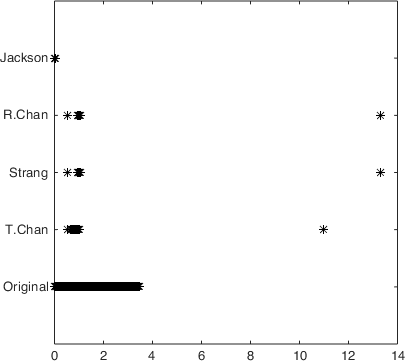
\includegraphics[width=0.87\columnwidth]{spectrum2.png}}%
\only<2>{$N = 1000$, $\alpha = 1.5$

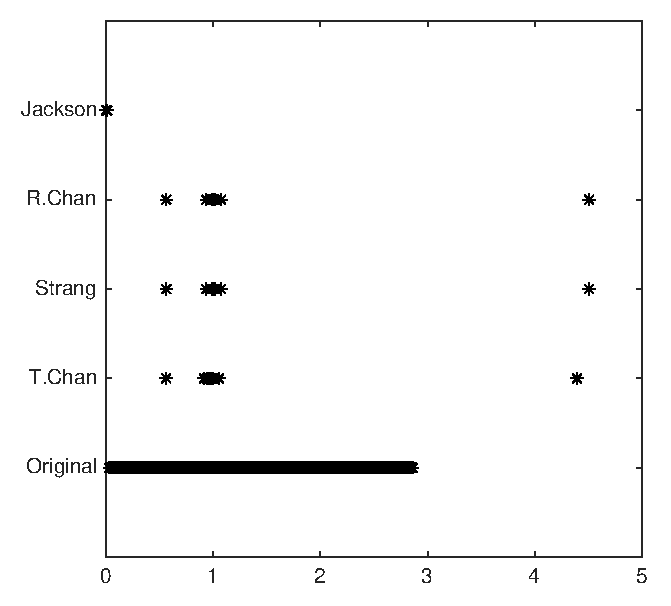
\includegraphics[width=0.87\columnwidth]{spectrum4.eps}
}%
\only<3->{$N = 1000$, $\alpha = 1.2$
	
	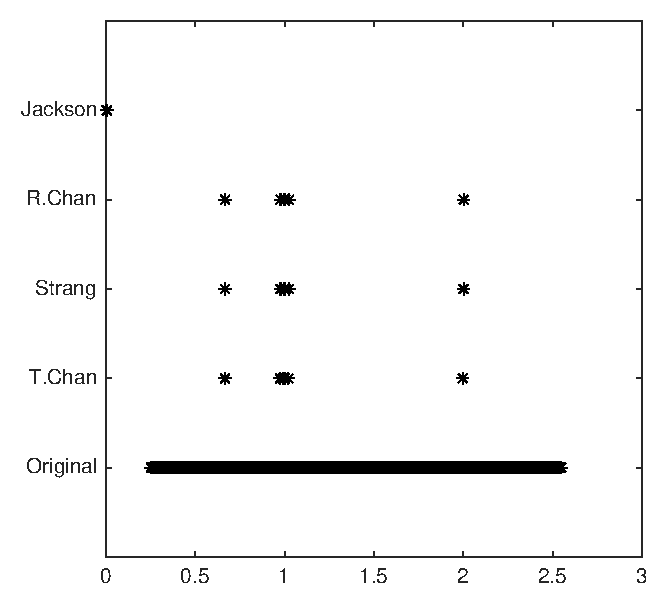
\includegraphics[width=0.87\columnwidth]{spectrum6.eps}
}
\end{column}
\end{columns}
\onslide<4>{\faQuestionCircle\,Can you guess what is happening with the Jackson Kernel preconditioner?}
\end{frame}

\begin{frame}{\faArrowDown\,A look at the convergence}

\begin{onlyenv}<1>
\begin{columns}
\begin{column}{0.5\columnwidth}
\begin{tabular}{lllllll}
\toprule
$\alpha$ & $N$ & PCG & Jackson & T.Chan & R.Chan & Strang \\
\midrule
\multirow{7}{*}{2.0} & $2^{5}$ & 15 & 6 & 8 & 2 & 2 \\
 & $2^{6}$ & 31 & 6 & 10 & 2 & 2 \\
 & $2^{7}$ & 63 & 6 & 12 & 2 & 2 \\
 & $2^{8}$ & 127 & 5 & 13 & 2 & 2 \\
 & $2^{9}$ & 251 & 5 & 14 & 2 & 2 \\
 & $2^{10}$ & 464 & 5 & 15 & 2 & 2 \\
 & $2^{11}$ & 713 & 4 & 15 & 2 & 2 \\
\bottomrule
\end{tabular}
\end{column}
\begin{column}{0.5\columnwidth}
\centering
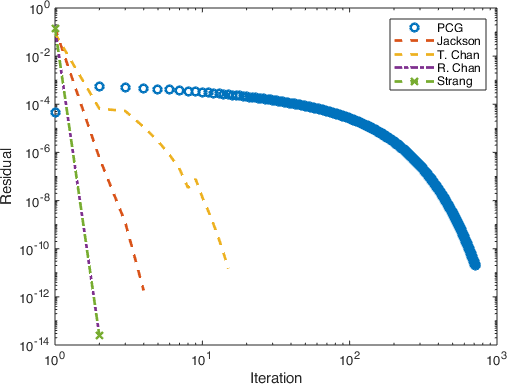
\includegraphics[width=0.9\columnwidth]{N=2048alpha=2.0.png}
\end{column}
\end{columns}
\end{onlyenv}
\begin{onlyenv}<2>
	\begin{columns}
		\begin{column}{0.5\columnwidth}
			\begin{tabular}{lllllll}
				\toprule
				$\alpha$ & $N$ & PCG & Jackson & T.Chan & R.Chan & Strang \\
				\midrule
				\multirow{7}{*}{1.8} & $2^{5}$ & 15 & 6 & 8 & 5 & 5 \\
				 & $2^{6}$ & 31 & 6 & 9 & 5 & 5 \\
				 & $2^{7}$ & 61 & 6 & 9 & 5 & 5 \\
				 & $2^{8}$ & 108 & 6 & 11 & 5 & 5 \\
				 & $2^{9}$ & 174 & 6 & 11 & 6 & 5 \\
				 & $2^{10}$ & 234 & 6 & 11 & 6 & 6 \\
				 & $2^{11}$ & 314 & 6 & 10 & 6 & 6 \\
				\bottomrule
			\end{tabular}
		\end{column}
		\begin{column}{0.5\columnwidth}
			\centering
			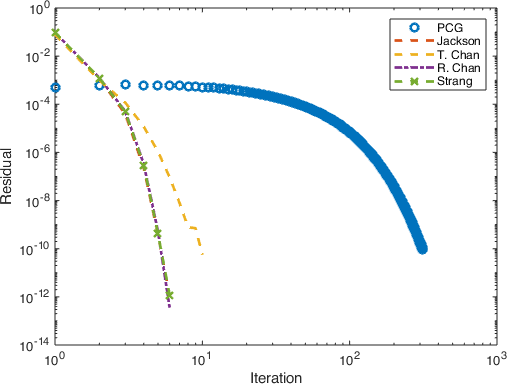
\includegraphics[width=0.9\columnwidth]{N=2048alpha=1.8.png}
		\end{column}
	\end{columns}
\end{onlyenv}
\begin{onlyenv}<3>
	\begin{columns}
		\begin{column}{0.5\columnwidth}
			\begin{tabular}{lllllll}
				\toprule
				$\alpha$ & $N$ & PCG & Jackson & T.Chan & R.Chan & Strang \\
				\midrule
				\multirow{7}{*}{1.6} & $2^{5}$ & 15 & 6 & 7 & 5 & 5 \\
				 & $2^{6}$ & 31 & 6 & 8 & 5 & 5 \\
				 & $2^{7}$ & 51 & 6 & 8 & 5 & 5 \\
				 & $2^{8}$ & 73 & 5 & 8 & 5 & 5 \\
				 & $2^{9}$ & 91 & 5 & 8 & 6 & 5 \\
				 & $2^{10}$ & 111 & 6 & 7 & 6 & 6 \\
				 & $2^{11}$ & 135 & 6 & 7 & 6 & 6 \\
				\bottomrule
			\end{tabular}
		\end{column}
		\begin{column}{0.5\columnwidth}
			\centering
			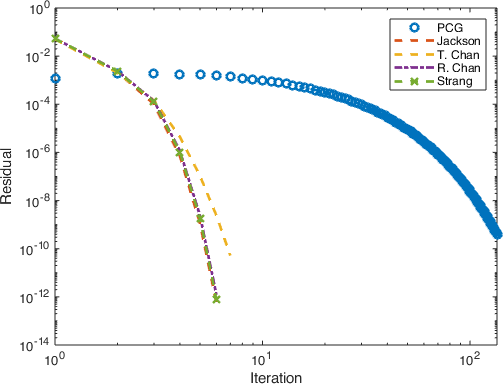
\includegraphics[width=0.9\columnwidth]{N=2048alpha=1.6.png}
		\end{column}
	\end{columns}
\end{onlyenv}
\begin{onlyenv}<4>
	\begin{columns}
		\begin{column}{0.5\columnwidth}
			\begin{tabular}{lllllll}
				\toprule
				$\alpha$ & $N$ & PCG & Jackson & T.Chan & R.Chan & Strang \\
				\midrule
				\multirow{7}{*}{1.4} & $2^{5}$ & 15 & 5 & 7 & 5 & 5 \\
				 & $2^{6}$ & 27 & 5 & 7 & 5 & 5 \\
				 & $2^{7}$ & 35 & 5 & 7 & 5 & 5 \\
				 & $2^{8}$ & 41 & 5 & 6 & 5 & 5 \\
				 & $2^{9}$ & 46 & 5 & 6 & 5 & 5 \\
				 & $2^{10}$ & 51 & 5 & 6 & 5 & 5 \\
				 & $2^{11}$ & 56 & 5 & 6 & 5 & 5 \\
				\bottomrule
			\end{tabular}
		\end{column}
		\begin{column}{0.5\columnwidth}
			\centering
			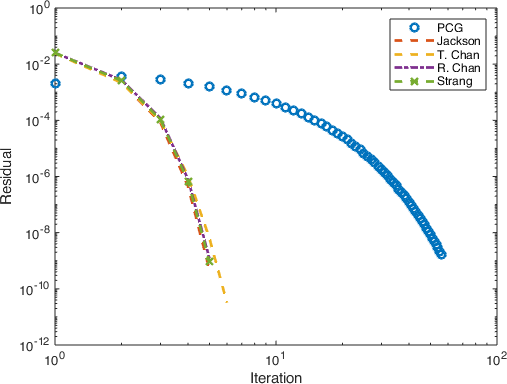
\includegraphics[width=0.9\columnwidth]{N=2048alpha=1.4.png}
		\end{column}
	\end{columns}
\end{onlyenv}
\begin{onlyenv}<5->
	\begin{columns}
		\begin{column}{0.5\columnwidth}
			\begin{tabular}{lllllll}
				\toprule
				$\alpha$ & $N$ & PCG & Jackson & T.Chan & R.Chan & Strang \\
				\midrule
				\multirow{7}{*}{1.2} & $2^{5}$ & 15 & 5 & 6 & 4 & 4 \\
				 & $2^{6}$ & 19 & 5 & 6 & 5 & 5 \\
				 & $2^{7}$ & 20 & 5 & 5 & 5 & 5 \\
				 & $2^{8}$ & 21 & 5 & 5 & 5 & 5 \\
				 & $2^{9}$ & 22 & 5 & 5 & 5 & 5 \\
				 & $2^{10}$ & 22 & 5 & 5 & 5 & 5 \\
				 & $2^{11}$ & 22 & 5 & 5 & 5 & 5 \\
				\bottomrule
			\end{tabular}
		\end{column}
		\begin{column}{0.5\columnwidth}
			\centering
			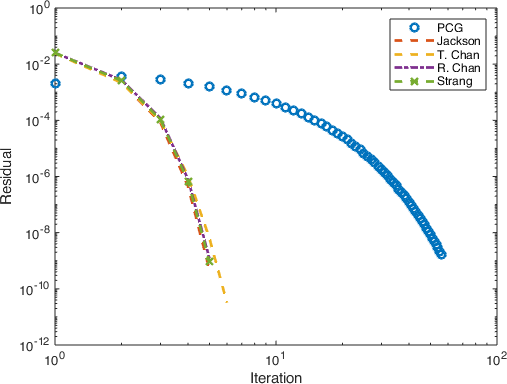
\includegraphics[width=0.9\columnwidth]{N=2048alpha=1.4.png}
		\end{column}
	\end{columns}
\end{onlyenv}
\onslide<6->{
\faEye\; We got \textbf{robustness} with respect to both $\alpha$ and $N$.
}

\onslide<7->{
\alert{\faQuestionCircle}\; What do we do in the \alert{non symmetric case}, i.e., $\theta \neq \nicefrac{1}{2}$?
}

\end{frame}

\subsection{Non symmetric Toeplitz system}

\begin{frame}{Non symmetric Toeplitz system}

If $T_n(f)$ is non symmetric (or more generally, non Hermitian), then $f$ is a complex-valued function then
\begin{itemize}
	\item[\faBomb] we \textbf{no longer} have information on the asymptotic \textbf{spectral distribution}, but only on the singular values,
	\item[\faBomb] we can \textbf{no longer} apply \textbf{fast} direct Toeplitz \textbf{solvers},
	\item[\faBomb] we can \textbf{no longer} apply the \textbf{CG} to $T_n(f)\mathbf{x} = \mathbf{b}$.
\end{itemize}
\alert{\faQuestionCircle}\; What to do?
\begin{itemize}
	\item[\faDoorOpen]<2-> Apply the PCG to the normal equations (CGNR):
	\[
	T_n(f)^H T_n(f) \mathbf{x} = T_n(f)^H \mathbf{b},
	\]
	\item[\faDoorOpen]<3-> Use another Krylov method: GMRES or TFQMR 
	
	\onslide<4->{ \faQuestionCircle[regular] do we know \alert{how to precondition} these methods? }
\end{itemize}

\end{frame}

\subsection{The GMRES method}

\begin{frame}{The GMRES method \parencite{GMRES}}

The \textbf{G}eneralized \textbf{M}inimum \textbf{Res}idual (GMRES) is a Krylov projection method
approximating the solution of linear system 
\[A\mathbf{x}=\mathbf{b}\] 
on the \textbf{affine subspace} 
\[\mathbf{x}^{(0)}+\mathcal{K}_m(A,\mathbf{v}_1), \quad \mathbf{r}^{(0)} = \mathbf{b}-A\,\mathbf{x}^{(0)}, \quad \mathbf{v}_1 = 
\nicefrac{\mathbf{r}^{(0)}}{\|\mathbf{r}^{(0)}\|_2} \],  
for $\mathbf{x}^{(0)}$ a \emph{starting guess} for the solution.

By this choice, we enforce the \textbf{Arnoldi relation}:
\begin{equation*}
	A\, V_m = V_m H_m+\mathbf{w}_m \mathbf{e}_m^T=V_{m+1}\overline{H}_m, \quad \operatorname{Span} V_m= \operatorname{Span}\{\mathbf{v}_1 \  \cdots \  \mathbf{v}_m\} = \mathcal{K}_m(A,\mathbf{v}_1),
\end{equation*}
and $H_m$ $m\times m$ Hessenberg submatrix extracted from $\overline{H}_m$ by deleting the $(m+1)$th
line.


\end{frame}

\begin{frame}{The GMRES method \parencite{GMRES}}
\begin{columns}
\begin{column}{0.4\columnwidth}
	\begin{algorithm}[H]\small
		\KwIn{$A\in \mathbb{R}^{n\times n}$,$\mathbf{b}\in \mathbb{R}^{n}$, $m$, $\mathbf{x}^{(0)}$} 
		$\mathbf{r}^{(0)} \leftarrow \mathbf{b}-A\,\mathbf{x}^{(0)}$, 
		$\beta\leftarrow\|\mathbf{r}^{(0)}\|_2$\; $\mathbf{v}_1\leftarrow
		\nicefrac{\mathbf{r}^{(0)}}{\beta}$\; 
		\For{$j=1,\ldots,m$}{
			$\mathbf{w}_j\leftarrow A\,\mathbf{v}_j$\; \
			\For{$i=1,\ldots,j$}{
				$h_{i,j}\leftarrow<\mathbf{w}_j,\mathbf{v}_i>$\;
				$\mathbf{w}_j\leftarrow\mathbf{w}_j-h_{i,j} \, \mathbf{v}_i$\; }
			$h_{j+1,j}\leftarrow\|\mathbf{w}_j\|_2$\; 
			\If{$h_{j+1,j}=0$ or \emph{convergence}}
			{ $m=j$\; 
				\textbf{break}\; 
			}
			$\mathbf{v}_{j+1}=\nicefrac{\mathbf{w}_j}{\|\mathbf{w}_j\|_2}$\; 
		} 
	\end{algorithm}
\end{column}
\begin{column}{0.6\columnwidth}
\begin{algorithm}[H]
Compute $\mathbf{y}^{(m)}$  such that
$\|\mathbf{r}^{(m)}\|_2=\|\mathbf{b}-A\,\mathbf{x}^{(m)}\|_2= \|\beta \mathbf{e}_1-\underline{H}_m
\mathbf{y}\|_2=\min_{\mathbf{y}\in\mathbb{R}^m}$\;
Build candidate approximation $\tilde{\textbf{x}}$\;
\end{algorithm}
\vspace{-0.5em}
\begin{block}<2->{Minimizing the residual}
At step $m$, the candidate solution $\mathbf{x}^{(m)}$ is the vector
minimizing the $2$--norm residual:\vspace{-0.5em}
\begin{equation*}
	\|\mathbf{r}^{(m)}\|_2=\|\mathbf{b}-A\,\mathbf{x}^{(m)}\|_2,\vspace{-0.5em}
\end{equation*}
with\vspace{-0.5em}
\[
\mathbf{b}-A\,\mathbf{x}^{(m)}  = V_{m+1} (\beta \textbf{e}_1 - \overline{H}_m \textbf{y}).
\]
\end{block}
\vspace{-0.5em}
\begin{block}<3->{GMRES variants}
\alert{Variants} obtained by different \alert{least square} problem \alert{solutions}, and \alert{different orthogonalization} algorithms.
\end{block}

\end{column}
\end{columns}
\end{frame}

\begin{frame}{The GMRES convergence theory (or lack thereof$\ldots$)}

\begin{alertblock}{Theorem (Convergence, diagonalizable)}
If  $A$ can be diagonalized, i.e. if we can find $X\in \mathbb{R}^{n
	\times n}$ non singular and such that
$$
A=X\,\Lambda\,X^{-1}, \  \Lambda=\operatorname{diag}(\lambda_1,\ldots,\lambda_n), \
K_2(X)=\|X\|_2\,\|X^{-1}\|_2,
$$
$K_2(X)=\|X\|_2\,\|X^{-1}\|_2$ condition number of $X$, then at step
$m$, we have
\begin{equation}\tag{DiagGMRES}
	\|r\|_2\leq K_2(X) \|\mathbf{r}^{(0)}\|_2
	\min_{\substack{\mathrm{p}(z)\in\mathbb{P}_m\\\mathrm{p}(0)=1}} \max_{i=1,\ldots,n}
	|\mathrm{p}(\lambda_i)|, \label{3:norm-res-GMRES}
\end{equation}
where $\mathrm{p}(z)$ is the polynomial of degree less or equal to  $m$
such that $\mathrm{p}(0)=1$ and the expression in the right hand side
of \eqref{3:norm-res-GMRES} is minimum.
\end{alertblock}

\begin{itemize}
	\item[\faExclamationTriangle] The \alert{eigenvectors} can be \alert{arbitrarily \emph{ill-conditioned}}, i.e., $K_2(X) \ggg 1$,
	\item[\faExclamationCircle] being \textbf{diagonalizable} can be a \textbf{strong assumption}.
\end{itemize}

\end{frame}

\begin{frame}{The GMRES convergence theory (or lack thereof$\ldots$)}

\begin{alertblock}{Theorem (Almostr everything is possible) \parencite{doi:10.1137/S0895479894275030}}
	Given a non-increasing positive sequence $\{f_k\}_{k=0,\ldots,n-1}$
	with $f_{n-1} > 0$ and a set of non--zero complex numbers
	$\{\lambda_i\}_{i=1,2,\ldots,n} \subset \mathbb{C}$, there exist a matrix $A$
	with eigenvalues $\lambda_1,\lambda_2,\ldots,\lambda_n$ and a
	right-hand side $\textbf{b}$ with $\|\textbf{b}\| = f_0$ such that the
	residual vectors $\textbf{r}^{(k)}$ at each step of the
	GMRES
	algorithm applied to solve $A\textbf{x} = \textbf{b}$ with
	$\textbf{x}^{(0)} = \textbf{0}$, satisfy $\|\textbf{r}^{(k)}\| = f_k$,
	$\forall \, k=1,2,\ldots,n-1$.
\end{alertblock}

\begin{itemize}
	\item[\faBomb] ``Any non-increasing convergence curve is possible for GMRES''.
	\item[\faQuestionCircle]<2-> What happens if we have \textbf{a clustered spectrum}?
	\item[\faLightbulb] In the clustered case we can partition $\sigma(A)$ as follows
	$$
	\sigma(A) = \sigma_c(A) \cup \sigma_{0}(A) \cup \sigma_{1}(A),
	$$
	where 
	\begin{itemize}
		\item $\sigma_c(A)$ denotes the \textbf{clustered set} of eigenvalues of $A$,
		\item $\sigma_{0}(A) \cup \sigma_{1}(A)$ denotes the \textbf{set of the
		outliers}.
	\end{itemize} 
\end{itemize}
\end{frame}

\begin{frame}{GMRES in the clustered and diagonalizable case}
\[
\sigma(A) = \underbrace{\sigma_c(A)}_{\text{clustered}} \cup \underbrace{\sigma_{0}(A) \cup \sigma_{1}(A)}_{\text{outliers}},
\]	
we assume that 
\begin{enumerate}
	\item the clustered set $\sigma_c(A)$ of eigenvalues is contained in a convex set $\Omega$,
	\item and, that denoting two sets of $j_0$ and $j_1$ outliers as
	\[
	\sigma_{0}(A) = \{ \hat{\lambda}_1, \hat{\lambda}_2, \ldots ,
	\hat{\lambda}_{j_0} \} \quad {\rm and} \quad \sigma_{1}(A) = \{
	\tilde{\lambda}_1, \tilde{\lambda}_2, \ldots , \tilde{\lambda}_{j_1} \}
	\]
	where if
	$\hat{\lambda}_j \in \sigma_{0}(A)$, we have
	$$
	1 < \left\lvert 1- \nicefrac{z}{\hat{\lambda}_j} \right\rvert \leq c_j, \quad
	\forall z \in \Omega,
	$$
	while, for $\tilde{\lambda}_j \in \sigma_{1}(A)$,
	$$
	0<\left\lvert 1- \nicefrac{z}{\tilde{\lambda}_j} \right\rvert < 1, \quad \forall
	z \in \Omega,
	$$
\end{enumerate}
\end{frame}

\begin{frame}{GMRES in the clustered and diagonalizable case}
\begin{alertblock}{Theorem}
The number of full GMRES iterations $j$ needed to attain a tolerance
$\varepsilon$ on the relative residual in the 2-norm
$\nicefrac{\|\mathbf{r}^{(j)}\|_2}{\|\mathbf{r}^{(0)}\|_2}$ for the linear system $A \mathbf{x} =\mathbf{b}$, where $A$ is
diagonalizable, is bounded above by
\begin{equation*}
	\min \left\{j_0+ j_1 + \left\lceil
	\frac{\log(\varepsilon)-\log(\kappa_2(X))}{\log(\rho)}-
	\sum_{\ell=1}^{j_0} \frac{\log(c_{\ell})}{\log(\rho)} \right\rceil,
	n\right\}, \label{bound-it-eig}
\end{equation*}
where
\begin{equation*}
	\rho^k=\frac{\left(a/d+\sqrt{(a/d)^2-1}\right)^k+\left(a/d+\sqrt{(a/d)^2-1}\right)^{-k}}
	{\left(c/d+\sqrt{(c/d)^2-1}\right)^k+\left(c/d+\sqrt{(c/d)^2-1}\right)^{-k}},
	\label{eq:ellipse-rho}
\end{equation*}
and the set $\Omega\in\mathbb{C}^+$ is the ellipse with center $c$,
focal distance $d$ and major semi axis $a$.
\end{alertblock}
\end{frame}

\begin{frame}{GMRES the non-diagonalizable case}

In this case we have to turn to either the \textbf{field of values} or the \textbf{$\varepsilon$-pseudospectra} of $A$.

We need to bound the right-hand side of
\[
\|\mathbf{r}_m\|_2\leq 
\min_{\substack{\mathrm{p}(z)\in\mathbb{P}_m\\\mathrm{p}(0)=1}} \|\mathrm{p}(A)\mathbf{r}_0\|, \quad m=1,2,\ldots
\]
or in the \alert{worst case scenario}
\[
\frac{\|\mathbf{r}_m\|_2}{\|\mathbf{r}_0\|} \leq \max_{\substack{\mathbf{v} \in \mathbb{C}^n\\\|\mathbf{v}\|=1}} \min_{\substack{\mathrm{p}(z)\in\mathbb{P}_m\\\mathrm{p}(0)=1}} \|\mathrm{p}(A)\mathbf{v}\| , \quad m=1,2,\ldots
\]
\begin{itemize}
	\item[\faCog] If $A$ is real, and $M = \nicefrac{(A+A^T)}{2}$ is SPD, then \parencite{MR694523}
	\[
	\max_{\substack{\mathbf{v} \in \mathbb{R}^n\\\|\mathbf{v}\|=1}} \min_{\substack{\mathrm{p}(z)\in\mathbb{P}_m\\\mathrm{p}(0)=1}} \|\mathrm{p}(A)\mathbf{v}\| \leq \left(1 - \frac{\lambda_{\min}(M)^2}{\lambda_{\max}(A^TA)}\right)^{\nicefrac{m}{2}}.
	\]
\end{itemize}
\end{frame}

\begin{frame}{GMRES the non-diagonalizable case}
\[
\|\mathbf{r}_m\|_2\leq 
\min_{\substack{\mathrm{p}(z)\in\mathbb{P}_m\\\mathrm{p}(0)=1}} \|\mathrm{p}(A)\mathbf{r}_0\|, \quad m=1,2,\ldots
\]
we recall that the \textbf{field of values} of $A$ is given by
\[
W(A) = \{ <A\mathbf{v},\mathbf{v}> \,:\, \mathbf{v} \in \mathbb{C}^n, \; \|\mathbf{v}\| = 1  \}, \qquad \nu(A) = \min_{z \in W(A)} |z|,
\]
with $\nu(A)$ the distance of $W(A)$ from the origin.
\begin{itemize}
	\item[\faCog]<2-> For a general nonsingular $A$ \parencite{MR2009695}
	\[
	\max_{\substack{\mathbf{v} \in \mathbb{C}^n\\\|\mathbf{v}\|=1}} \min_{\substack{\mathrm{p}(z)\in\mathbb{P}_m\\\mathrm{p}(0)=1}} \|\mathrm{p}(A)\mathbf{v}\| \leq ( 1 - \nu(A)\nu(A^{-1}) )^{\nicefrac{m}{2}}.
	\]
	\item[\alert{\faExclamationTriangle}]<3-> This bound is useful only when $0 \notin W(A)$ and $0 \notin W(A^{-1})$.
\end{itemize}
\end{frame}

\begin{frame}{Some experimentation with the FOV in our case}
\[
\nu_N^{\alpha-1} A_N = \nu_N^{\alpha-1} I_N - \theta G_N + (1-\theta)G_N^T,
\]
\only<1>{\begin{columns}
\begin{column}{0.5\columnwidth}
\centering
$\theta = 0.2$, $\alpha=1.2$, $N=100$

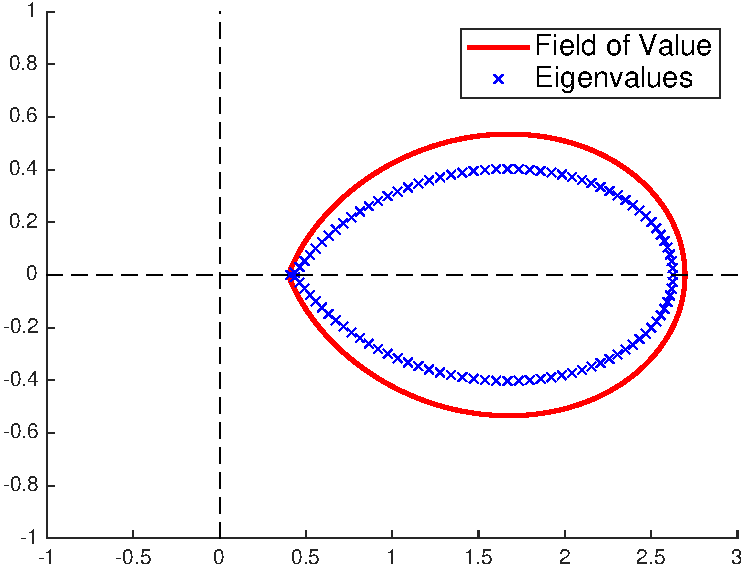
\includegraphics[width=0.95\columnwidth]{fovcase1.pdf}
\end{column}
\begin{column}{0.5\columnwidth}
\centering
$\theta = 0.2$, $\alpha=1.2$, $N=1000$

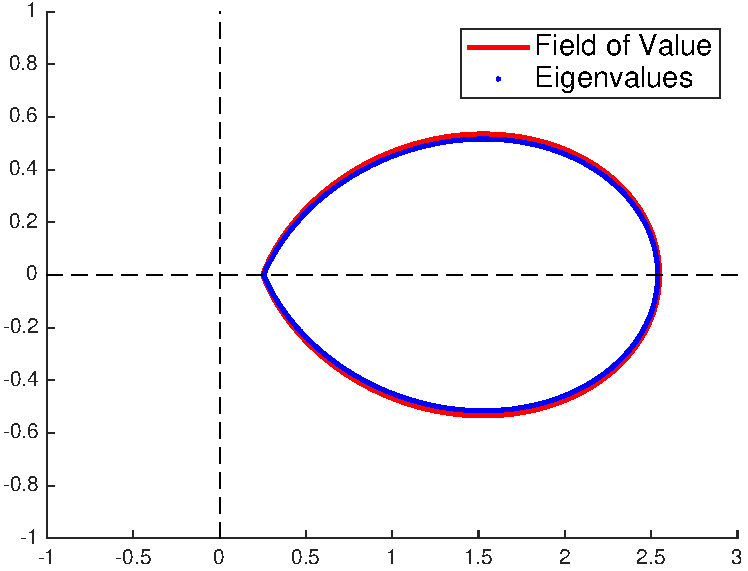
\includegraphics[width=0.95\columnwidth]{fovcase2.pdf}	
\end{column}
\end{columns}}
\only<2->{\begin{columns}
		\begin{column}{0.5\columnwidth}
			\centering
			$\theta = 0.2$, $\alpha=1.8$, $N=100$
			
			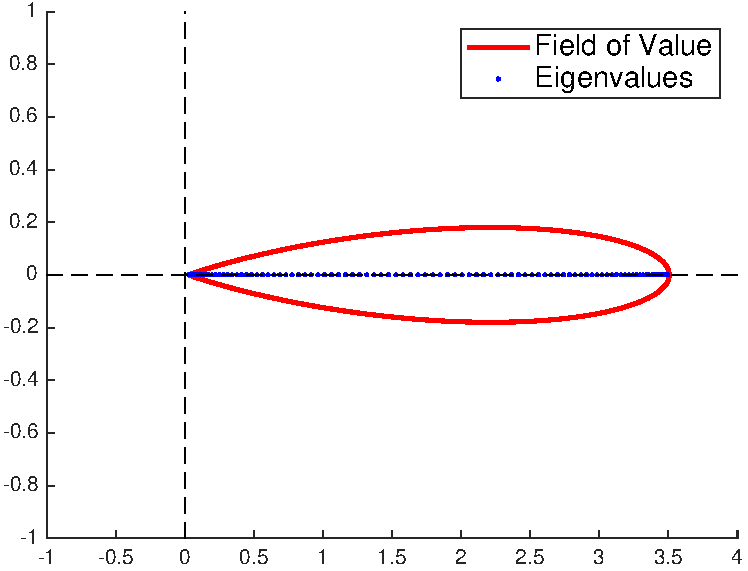
\includegraphics[width=0.95\columnwidth]{fovcase3.pdf}
		\end{column}
		\begin{column}{0.5\columnwidth}
			\centering
			$\theta = 0.2$, $\alpha=1.8$, $N=1000$
			
			\only<2>{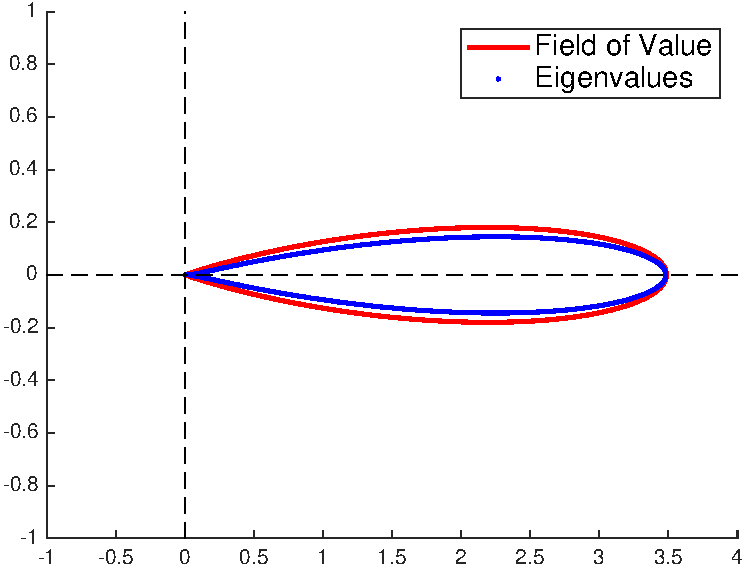
\includegraphics[width=0.95\columnwidth]{fovcase4.pdf}}%
			\only<3>{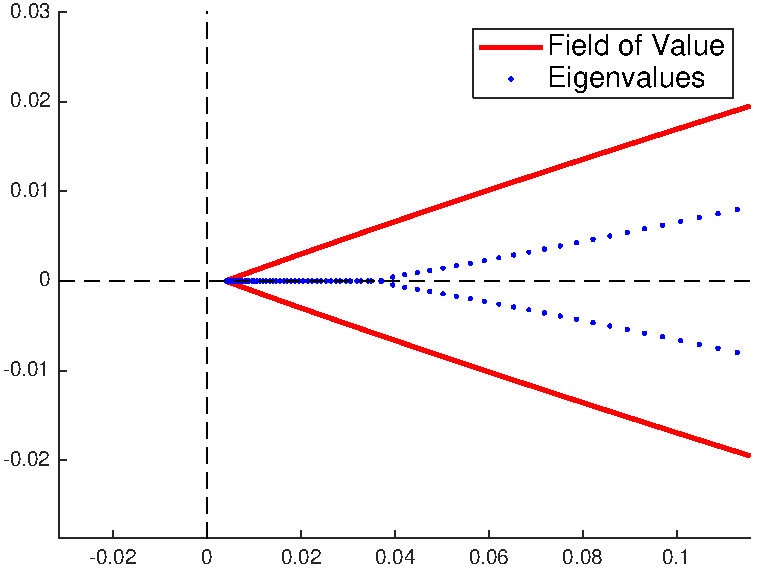
\includegraphics[width=0.95\columnwidth]{fovcase4bis.pdf}}
		\end{column}
\end{columns}}

\end{frame}

\begin{frame}{Some experimentation with the FOV in our case}

\begin{exampleblock}{\faSadTear\,Unfortunate truth}
In general it is difficult to say something about the Field of Value of preconditioned matrices.
\end{exampleblock}

\begin{itemize}
	\item[\faQuestionCircle]<2-> What do we do in practice?
	\begin{quote}
		``To speed up the CG-like methods, we can choose a matrix $C$ such that the singular values of the preconditioned matrix $C^{-1}A$ are clustered.'' -- \parencite[P. 439]{MR1409592}
	\end{quote}
	\item[\faQuestionCircle]<3-> How do we build a \textbf{Circulant preconditioner} for a \textbf{our non-symmetric Toeplitz} matrix?
	\item[\faLightbulb]<4-> We can use a suitably modified Strang preconditioner for our case \parencite{MR3062056}
\end{itemize}

\end{frame}

\begin{frame}[fragile]{\faHammer\,A Circulant preconditioner \parencite{MR3062056}}

\begin{columns}
\begin{column}{0.5\columnwidth}
We can build a circulant preconditioner as
\[
P = \frac{h_N^\alpha}{\Delta t} I_{N} + \theta \alert<1>{s(G_{N})} + (1-\theta) \alert<2>{s(G_{N}^T)},
\]
\only<1-2>{where\vspace{-1em}
\[
\only<1>{(s(G_N))_{:,1} = - \begin{bmatrix}
g_1^{(\alpha)} \\
\vdots \\
g_{\lfloor \nicefrac{(N+1)}{2} \rfloor}^{\alpha} \\
0 \\
\vdots \\
0 \\
g_0^{(\alpha)} 
\end{bmatrix},}\only<2>{(s(G_N^T))_{:,1} = - \begin{bmatrix}
g_1^{(\alpha)} \\
g_0^{(\alpha)} \\
0 \\
\vdots \\
0 \\
g_{\lfloor \nicefrac{(N+1)}{2} \rfloor}^{\alpha} \\
\vdots \\
g_2^{(\alpha)} 
\end{bmatrix}.}
\]}\only<3-4>{\vspace{-1em}
\begin{itemize}
	\item[\faCog] It uses the \textbf{construction of the Strang preconditioner} using only \emph{half o the bandwidth} of the Toeplitz matrices.
	\item[\faCog]<4-> All the eigenvalues of $s(G_N)$ and $s(G_N^T)$ fall inside the open disc $\{z \in \mathbb{C} \,:\, |z-\alpha| < \alpha\}$ by Gershgorin theorem, indeed:\vspace{-0.8em}
	\[
	\hspace{-1em}r_N = g_0^{\alpha} + \sum_{k=2}^{\lfloor \nicefrac{(N+1)}{2} \rfloor} < \sum_{\substack{k = 0\\k\neq 1}} g_k^{(\alpha)} = - g_1^{(\alpha)} = \alpha.
	\]
\end{itemize}
}%
\only<5>{
\centering

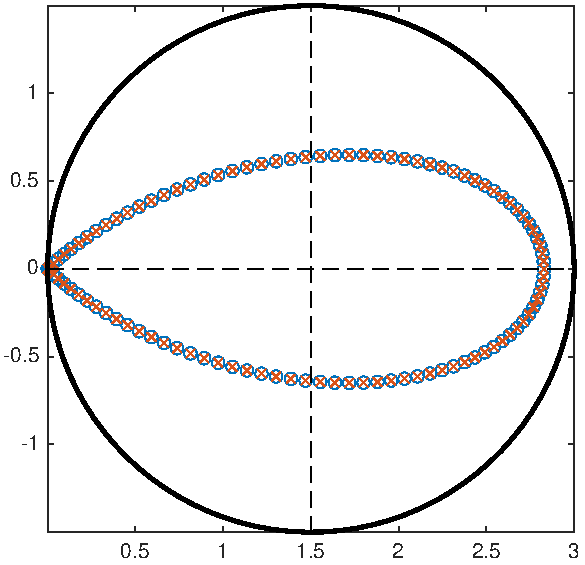
\includegraphics[width=0.65\columnwidth]{strangev.pdf}
}
\end{column}
\begin{column}{0.5\columnwidth}
\definecolor{bg}{rgb}{0.95,0.95,0.95}
\begin{minted}[bgcolor=bg,fontsize=\small,breaklines]{matlab}
function [ev,evt] = sunprec(N,alpha)
g = gl(N,alpha);
v = zeros(N,1);
v(1:floor((N+1)/2)) = g((1:floor((N+1)/2))+1);
v(end) = g(1);
ev = fft(-v);
v = zeros(N,1);
v(1) = g(2);
v(2) = g(1);
v(end:-1:floor((N+1)/2)+2) = g(3:floor((N+1)/2)+1);
evt = fft(-v);
end
\end{minted}
\end{column}
\end{columns}

\end{frame}

\begin{frame}[fragile]{\faHammer\,A Circulant preconditioner \parencite{MR3062056}}
\faQuestionCircle\;Will it work?

We can always write:
\[
P^{-1} A_{N} - I_N = P^{{-1}} ( A_N - P) \onslide<2->{ = \alert<3>{P_N^{-1} U_N} - \alert<5>{P_N^{-1} V_N}} \only<6>{ \Rightarrow \text{``small rank'' }+\text{ ``small norm''}},
\]
now for the Strang preconditioner of a Toeplitz matrix with with generating function in the Wiener class, it holds that for any $\varepsilon > 0$ exists $N'$ and $M'$ such that
\[
A_N - s(A_N) = U_N + V_N, \quad \operatorname{rank}(U_N) \leq M' \text{ and } \|V_N\|_2 < \varepsilon \; \forall N > N'.
\]\vspace{-1em}
\begin{itemize}
	\item[\faWrench]<3-> $\operatorname{rank}(P_N^{-1} U_N) \leq \operatorname{rank}(U_N) \leq M'$,
	\only<4>{\item[\faCog]<4-> $\forall\,k=1,2,\ldots,N$, $ | \lambda(P_N) | \geq \Re( \Lambda(P_N)_{k,k} ) = \nicefrac{h_N^\alpha}{\Delta t} + \theta \Re( \Lambda( s(G_N) )_{kk}  ) + (1-\theta) \Re( \Lambda(s(G_N^T))_{kk} ) \geq \nicefrac{h_N^\alpha}{\Delta t}  > 0$ and thus $\| P^{-1}_N \|_2 \leq \nicefrac{\Delta t}{h_N^\alpha}$}
	\only<5->{
	\item[\faWrench] $\|P_N^{-1} V_N \| \leq \| P_N^{-1} \|_2 \| V_N \|_2 < \nicefrac{\varepsilon \Delta t}{ h_N^\alpha }$.
	\item[\faLightbulb]<6-> If we select $\Delta t$ and $h_N$ in such a way that $\nicefrac{h_N^\alpha}{\Delta t}$ is bounded and bounded away from zero we have the result.
	}
\end{itemize}


\end{frame}


\begin{frame}[fragile]{Results with GMRES}
\definecolor{bg}{rgb}{0.95,0.95,0.95}
\only<1>{
\[
\left( \frac{h_N^\alpha}{\Delta t} I_{N-2} -  \left[ \theta G_{N-2} + (1-\theta) G_{N-2}^T \right] \right) \mathbf{w}^{n+1} =\frac{h_N^\alpha}{\Delta t}, \quad \theta = 0.2
\]}
\begin{onlyenv}<2->
\begin{minted}[bgcolor=bg,fontsize=\small,breaklines]{matlab}
[ev,evt] = sunprec(N,alpha);
c = nu + theta*ev + (1-theta)*evt;
P = @(x) cprec(c,x);
[X,FLAGsun,RELRESsun,ITERsun,RESVECsun] = gmres(A,(nu*w),[],1e-9,N,P);
\end{minted}
\end{onlyenv}
\onslide<2>{
\begin{columns}
\begin{column}{0.25\columnwidth}
\begin{tabular}{llcl}
\toprule
$\alpha$ & $N$ & GMRES & P \\
\midrule
\multirow{7}{*}{1.2} & $2^{5}$ & 28 & 6 \\
& $2^{6}$ & 31 & 6 \\
& $2^{7}$ & 33 & 6 \\
& $2^{8}$ & 34 & 6 \\
& $2^{9}$ & 35 & 6 \\
& $2^{10}$ & 36 & 6 \\
& $2^{11}$ & 36 & 6 \\
\bottomrule
\end{tabular}
\end{column}

\begin{column}{0.25\columnwidth}
\begin{tabular}{llcl}
\toprule
$\alpha$ & $N$ & GMRES & P \\
\midrule
\multirow{7}{*}{1.4} & $2^{5}$ & 31 & 6 \\
& $2^{6}$ & 46 & 6 \\
& $2^{7}$ & 54 & 6 \\
& $2^{8}$ & 62 & 7 \\
& $2^{9}$ & 69 & 7 \\
& $2^{10}$ & 78 & 7 \\
& $2^{11}$ & 87 & 7 \\
\bottomrule
\end{tabular}
\end{column}

\begin{column}{0.25\columnwidth}
\begin{tabular}{llcl}
\toprule
$\alpha$ & $N$ & GMRES & P \\
\midrule
\multirow{7}{*}{1.6} & $2^{5}$ & 32 & 6 \\
& $2^{6}$ & 59 & 6 \\
& $2^{7}$ & 82 & 7 \\
& $2^{8}$ & 105 & 7 \\
& $2^{9}$ & 128 & 7 \\
& $2^{10}$ & 156 & 7 \\
& $2^{11}$ & 189 & 7 \\
\bottomrule
\end{tabular}
\end{column}

\begin{column}{0.25\columnwidth}
\begin{tabular}{llcl}
\toprule
$\alpha$ & $N$ & GMRES & P \\
\midrule
\multirow{7}{*}{1.8} & $2^{5}$ & 32 & 6 \\
& $2^{6}$ & 64 & 6 \\
& $2^{7}$ & 109 & 6 \\
& $2^{8}$ & 162 & 7 \\
& $2^{9}$ & 222 & 7 \\
& $2^{10}$ & 287 & 7 \\
& $2^{11}$ & 372 & 7 \\
\bottomrule
\end{tabular}
\end{column}

\end{columns}}

\end{frame}


\section{Conclusion and summary}

\begin{frame}{Conclusion and summary}
	\definecolor{success}{HTML}{4a934a}
	\definecolor{todo}{HTML}{0099cc}
	
	\begin{itemize}
		\item[\textcolor{success}{\faCheckCircle}] We have discussed the solution of Toeplitz linear systems,
		\item[\textcolor{success}{\faCheckCircle}] Studied the usage and convergence of PCG and GMRES method,
		\item[\textcolor{success}{\faCheckCircle}] Tested the usage of Circulant preconditioners for Toeplitz linear systems.
	\end{itemize}

Next up
	\begin{itemize}
		\item[\textcolor{todo}{\faClipboardList}] We need to discuss the next problem in difficulty
		\begin{equation*}
			\begin{cases}\frac{\partial W}{\partial t} = \alert{d^+(x,t)} \,{}^{\only<1>{RL}}D_{[0,x]}^\alpha W(x,t) + \alert{d^-(x,t)} {}^{\only<1>{RL}}D_{[x,1]}^\alpha W(x,t), \qquad \theta \in [0,1],\\
				W(0,t) = W(1,t) = 0, \qquad W(x,t) = W_0(x).	
			\end{cases}
		\end{equation*}
		\item[\textcolor{todo}{\faClipboardList}] What happens if we go to \textbf{more than one spatial dimension}?
	\end{itemize}

\end{frame}

\appendix

\section*{Bibliography}
{\unnumbered
	\begin{frame}[allowframebreaks,noframenumbering]{Bibliography}
	\small
	\printbibliography
	
\end{frame}
}

\end{document}